\noindent
\LARGE \textbf{Supplementary Material}

\label{supp_results}

\maketitle

\normalsize
\setcounter{section}{0}
\section{Application}
\label{App_Application}
\begin{figure}[!ht]
\centering
\caption{Outcome \textit{seizure freedom}: comparison of naive and univariate ORB-adjusted estimates for selection on the log OR/log RR and on the $z$-score over increasing selection.}
\label{fig:OR_RR_REM}
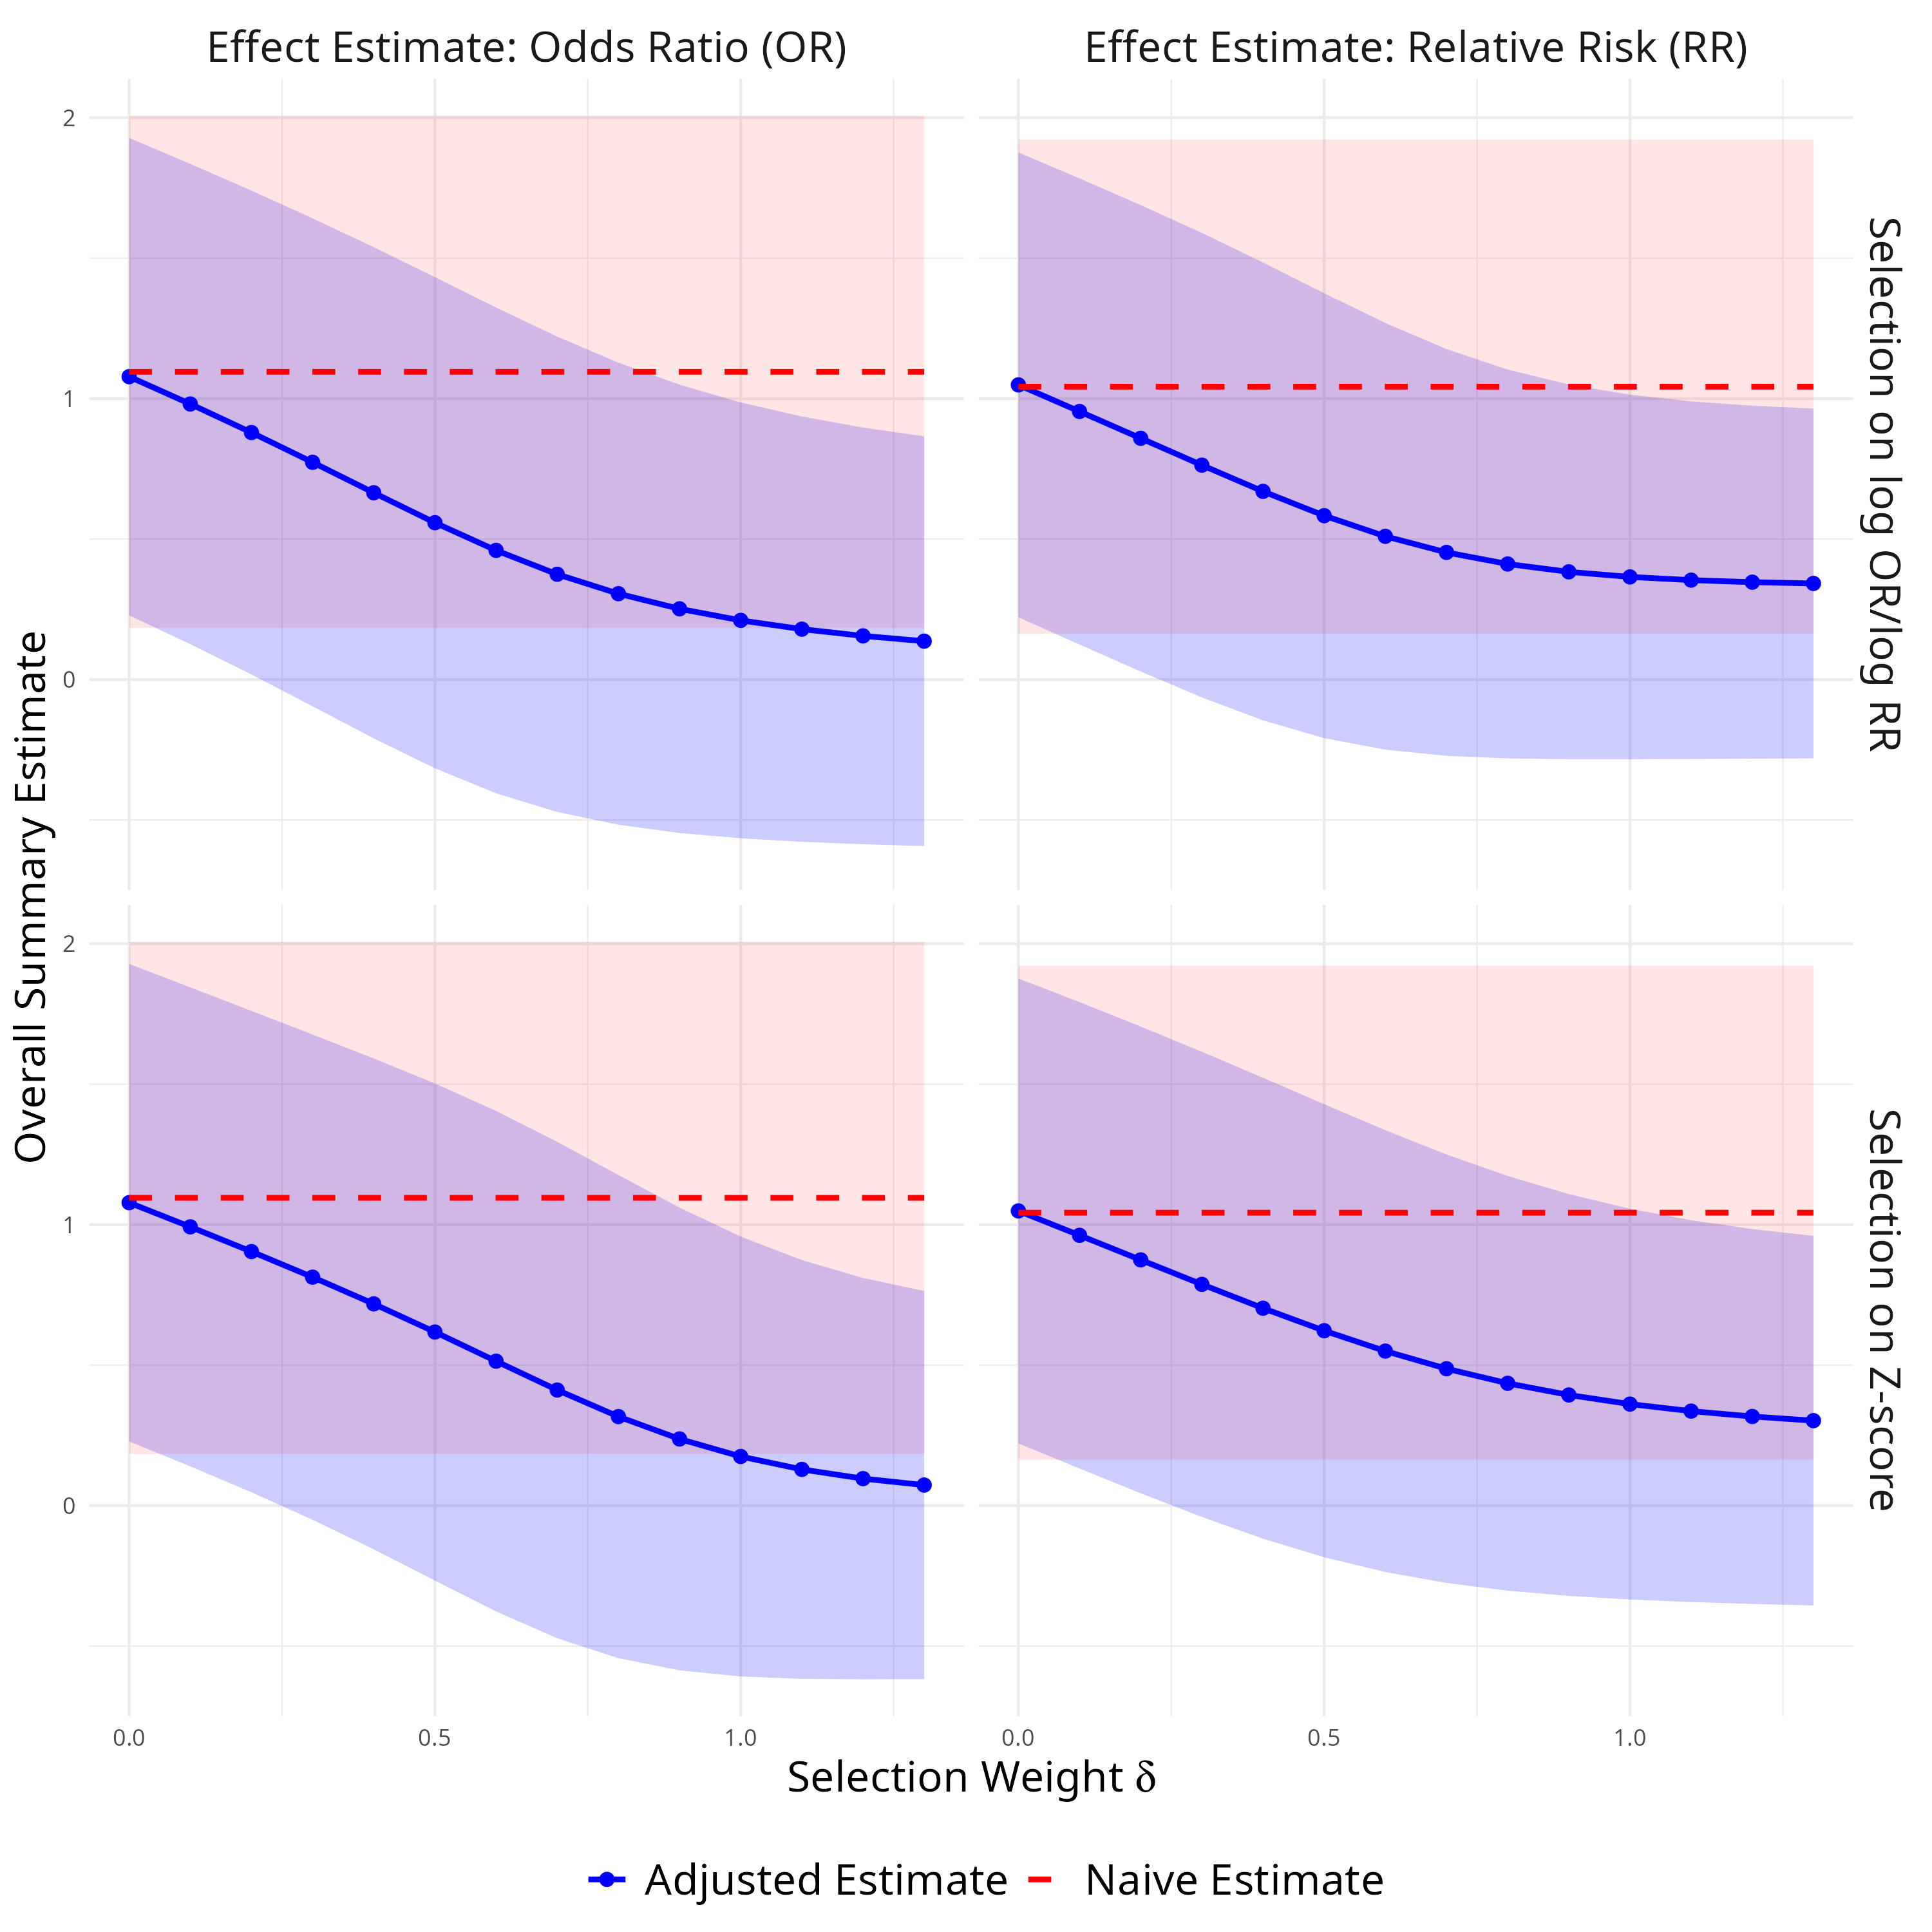
\includegraphics[width = 1\linewidth]{figures/App_Uni_REM_O2.png}
\end{figure}
\noindent
Figure \ref{fig:OR_RR_REM} shows how large the overestimation of the treatment effect is for \textit{seizure freedom} for increasing selection. Selection on the $z$-score results in slightly lower adjusted estimates than treatment effect selection. Differences between OR and RR are small but consistent, with OR yielding slightly larger estimates and wider CIs. With increasing $\delta$ (\ie $\delta > 0.8$), the adjusted OR decreases more sharply on the $z$-score selection since studies with larger standardized effects are preferentially retained, producing a stronger adjustment as the assumed selection strength increases.


\begin{figure}[ht!]
\centering
\caption{Outcome \textit{50\% seizure reduction}: comparison of naive and univariate ORB-adjusted estimates for selection on the log OR/ log RR and selection on the $z$-score over increasing selection.}
\label{fig:Univariate2}
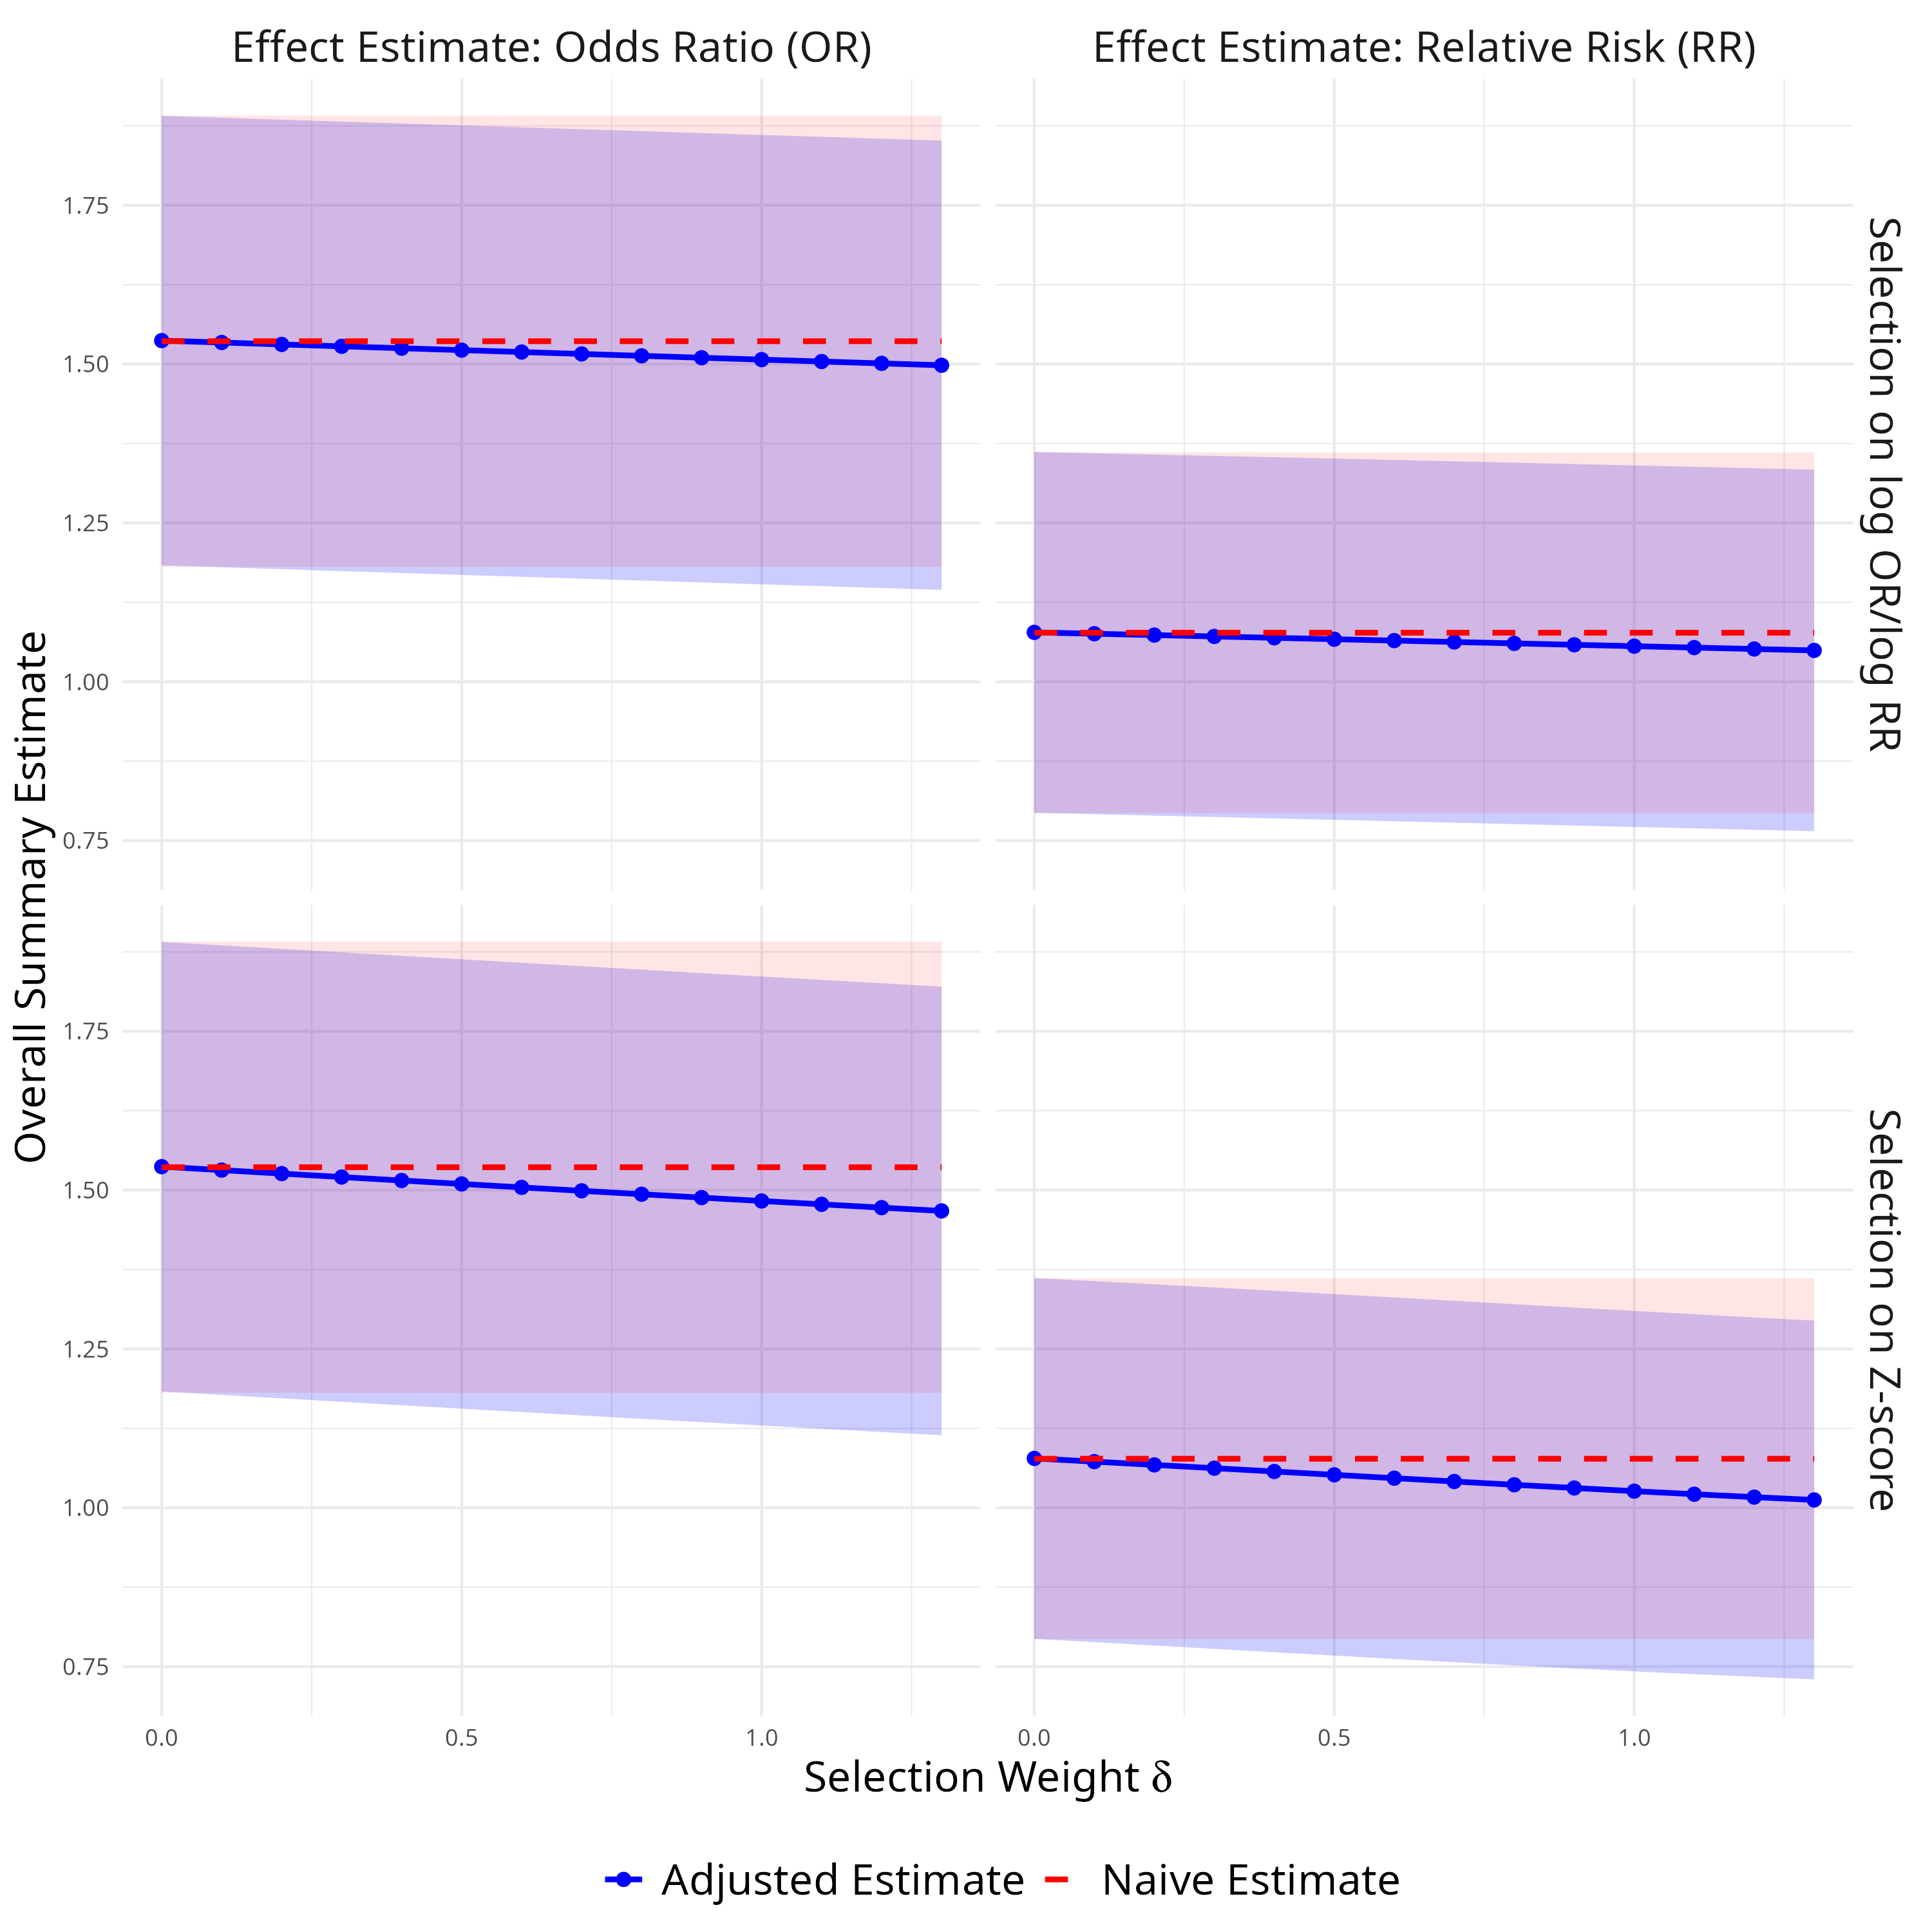
\includegraphics[width = 1\linewidth]{figures/App_Uni_REM_O1.png}
\end{figure}

In the manuscript, we focused primarily on the outcome \textit{seizure freedom} as it has more unreported study outcomes and therefore provides a clearer visualization of our ORB adjustment method. For completeness, this section presents the corresponding plots for the second outcome \textit{50\% seizure reduction}.
As expected, the ORB-adjusted treatment effects and corresponding CIs are generally shifted toward the null compared to the naive MA estimates based only on the reported studies (Figure \ref{fig:Univariate2}). However, because only one study outcome is unreported for \textit{50\% seizure reduction}, the magnitude of the adjustment is substantially smaller than for \textit{seizure freedom}, where approximately half of the study outcomes are unreported. Consequently, the CIs of the naive and adjusted estimates are very similar. For both the OR and RR, selection on the $z$-score produces slightly stronger adjustment than selection on the effect estimate. This reflects the dependence of $z$-score selection on both the treatment effect and its standard error, giving greater influence to more precise studies as the selection weight increases. Similar to the findings for \textit{seizure freedom}, the OR estimates remain larger and have wider CIs  than the RR estimates. Overall, however, the differences between naive and adjusted estimates remain modest because the proportion of unreported study outcomes is small.

\begin{figure}[ht!]
\centering
\caption{Outcome \textit{50\% seizure reduction}: comparison of univariate and multivariate ORB-adjustment (for a correlation of $r = -0.3$) for selection on the log OR/ log RR and selection on the $z$-score over increasing selection.}
\label{fig:Uni_Multi_O1}
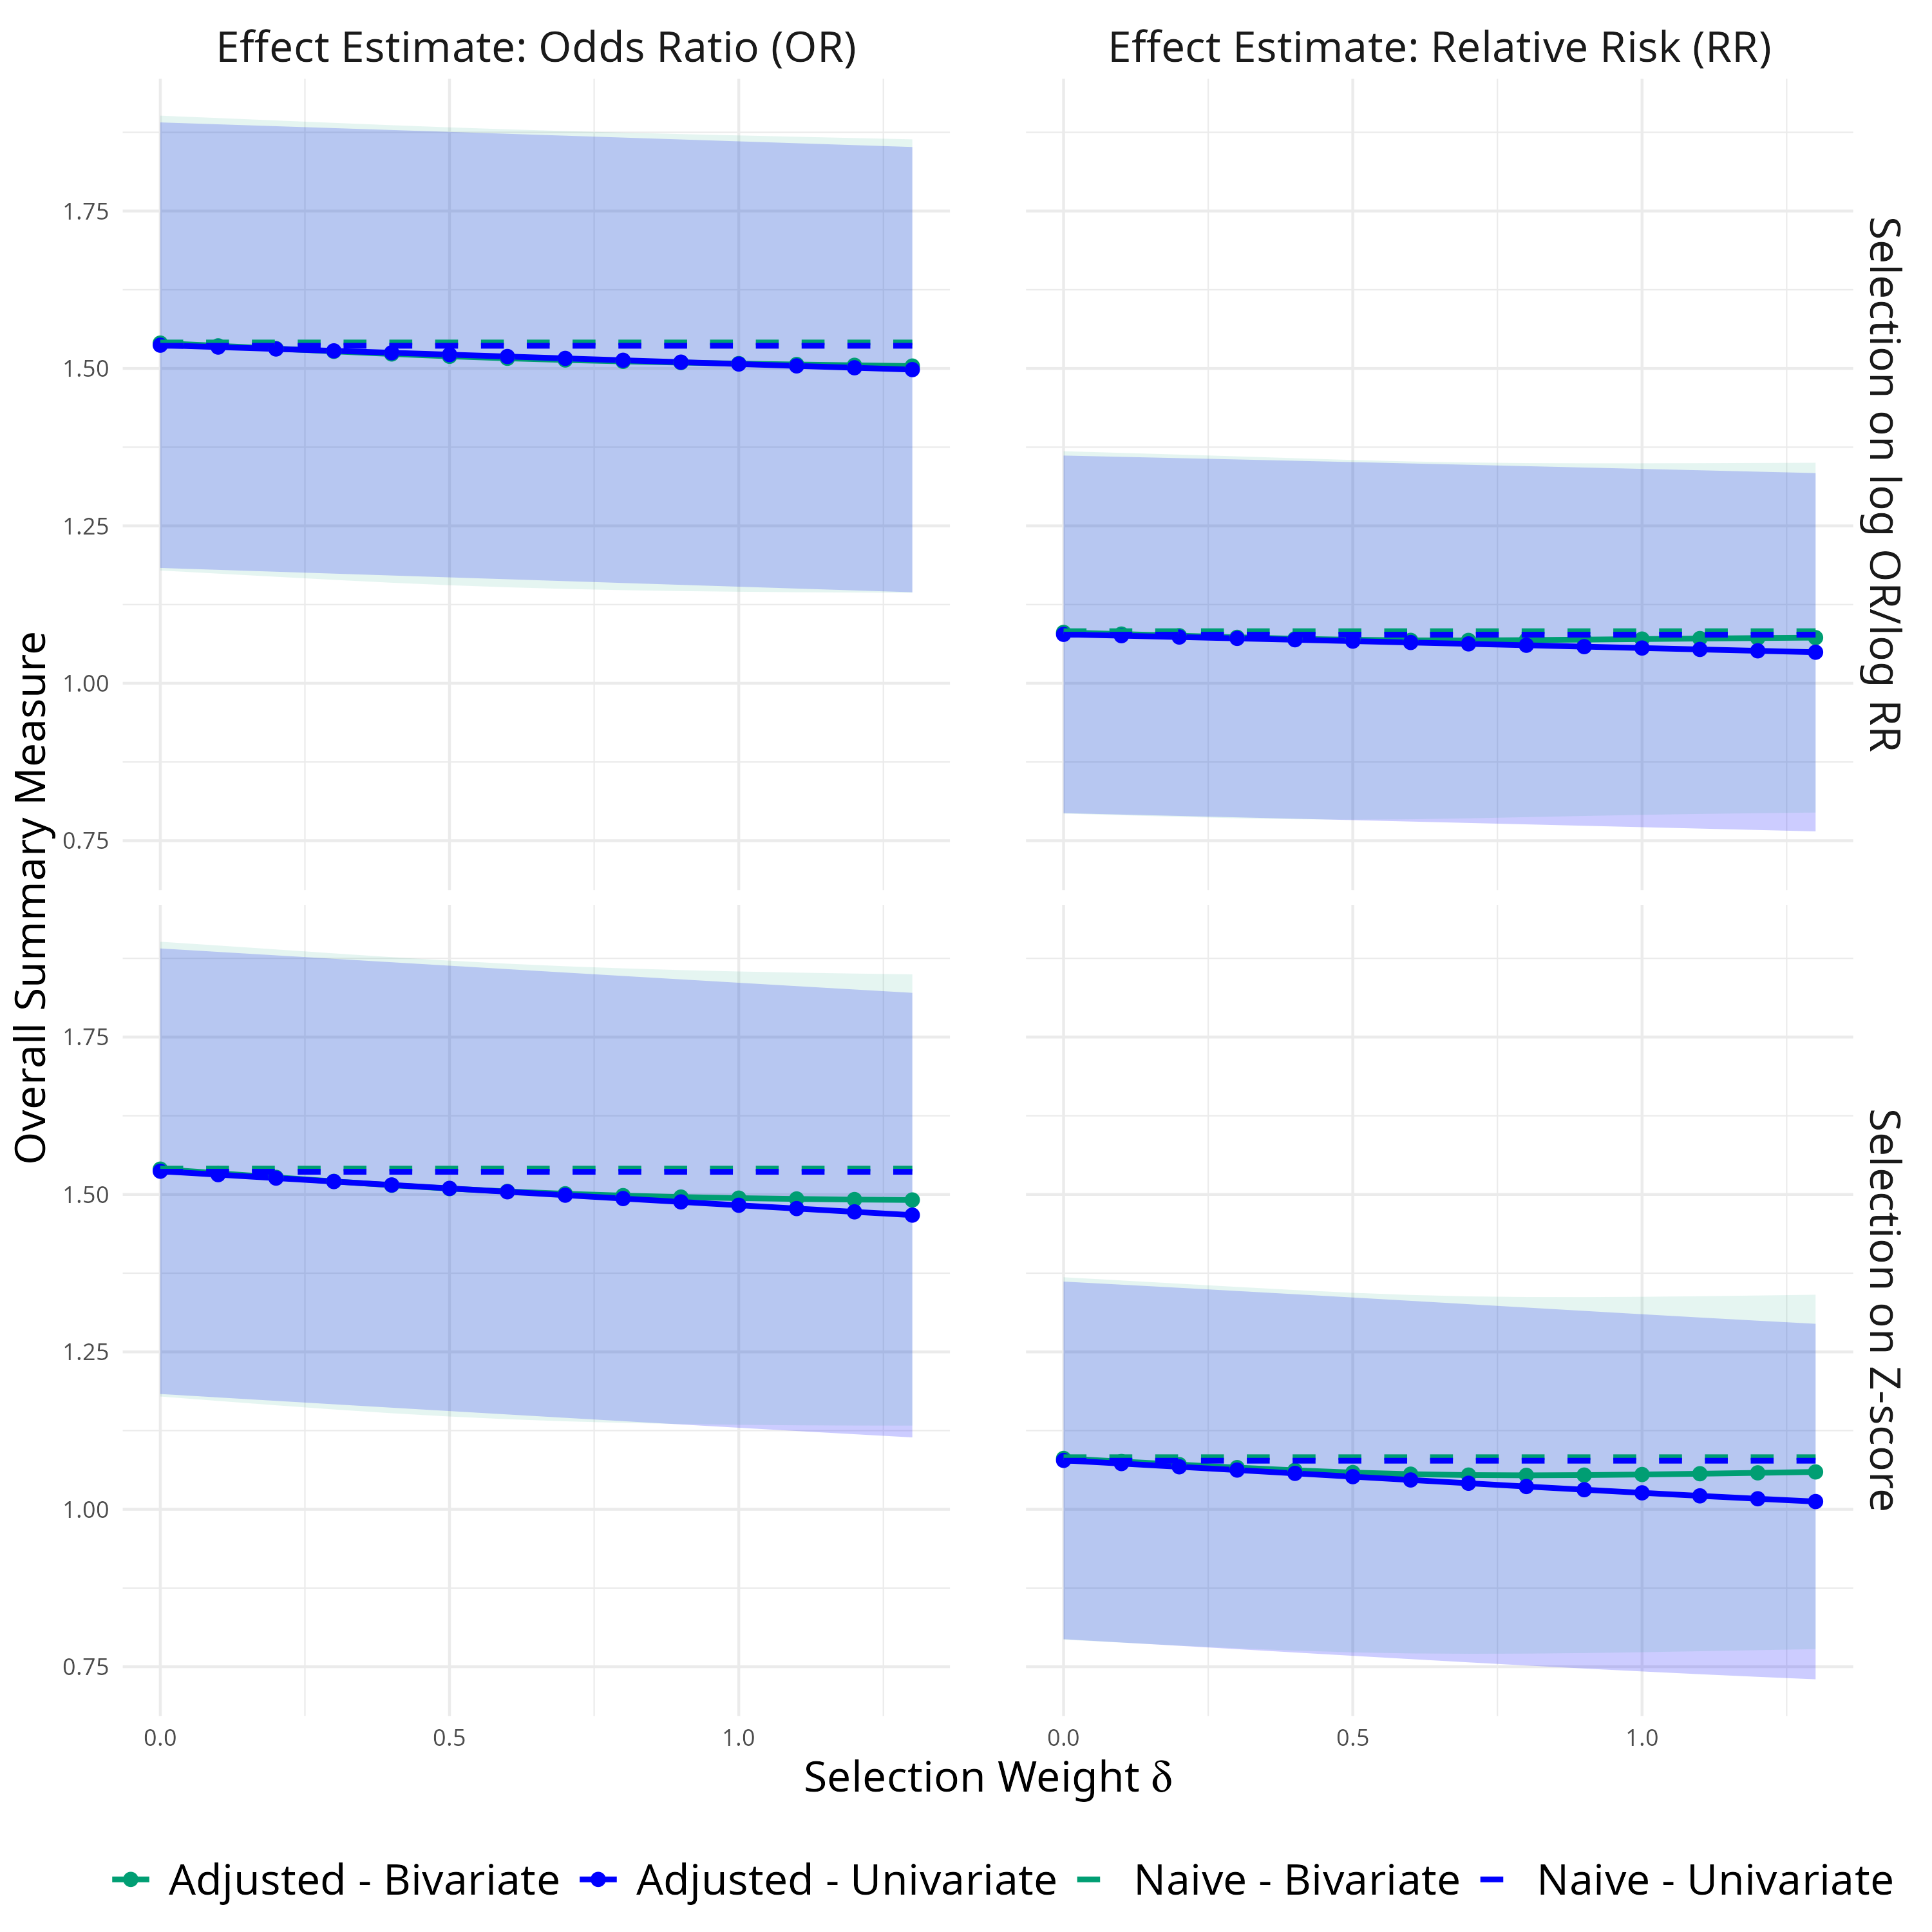
\includegraphics[width = 1\linewidth]{figures/Uni_Multi_Comp_12_REM_01.png}
\end{figure}

Next, we compared the univariate and multivariate ORB adjustment for the outcome \textit{50\% seizure reduction}, assuming a fixed within-study correlation of -0.3 (see Figure~\ref{fig:Uni_Multi_O1}). The dashed lines represent the naive MA estimates based only on the reported studies. These estimates differ between the univariate and multivariate approach because the multivariate model jointly incorporates both outcomes and their covariance structure. Across all scenarios, the adjusted estimates decrease with increasing selection, reflecting stronger assumed ORB. In contrast to the stronger differences observed for \textit{seizure freedom}, the univariate and multivariate adjustments for \textit{50\% seizure reduction} remain relatively similar, with largely overlapping CIs. For selection on the $z$-score, the univariate adjustment is slightly stronger than for selection on the effect estimate.

\begin{figure}[ht!]
\centering
\caption{Outcome \textit{50\% seizure reduction}: comparison of within-study correlations for multivariate ORB-adjustment for selection on the log OR/ log RR and selection on the $z$-score over increasing selection.}
\label{fig:Multivariate2}
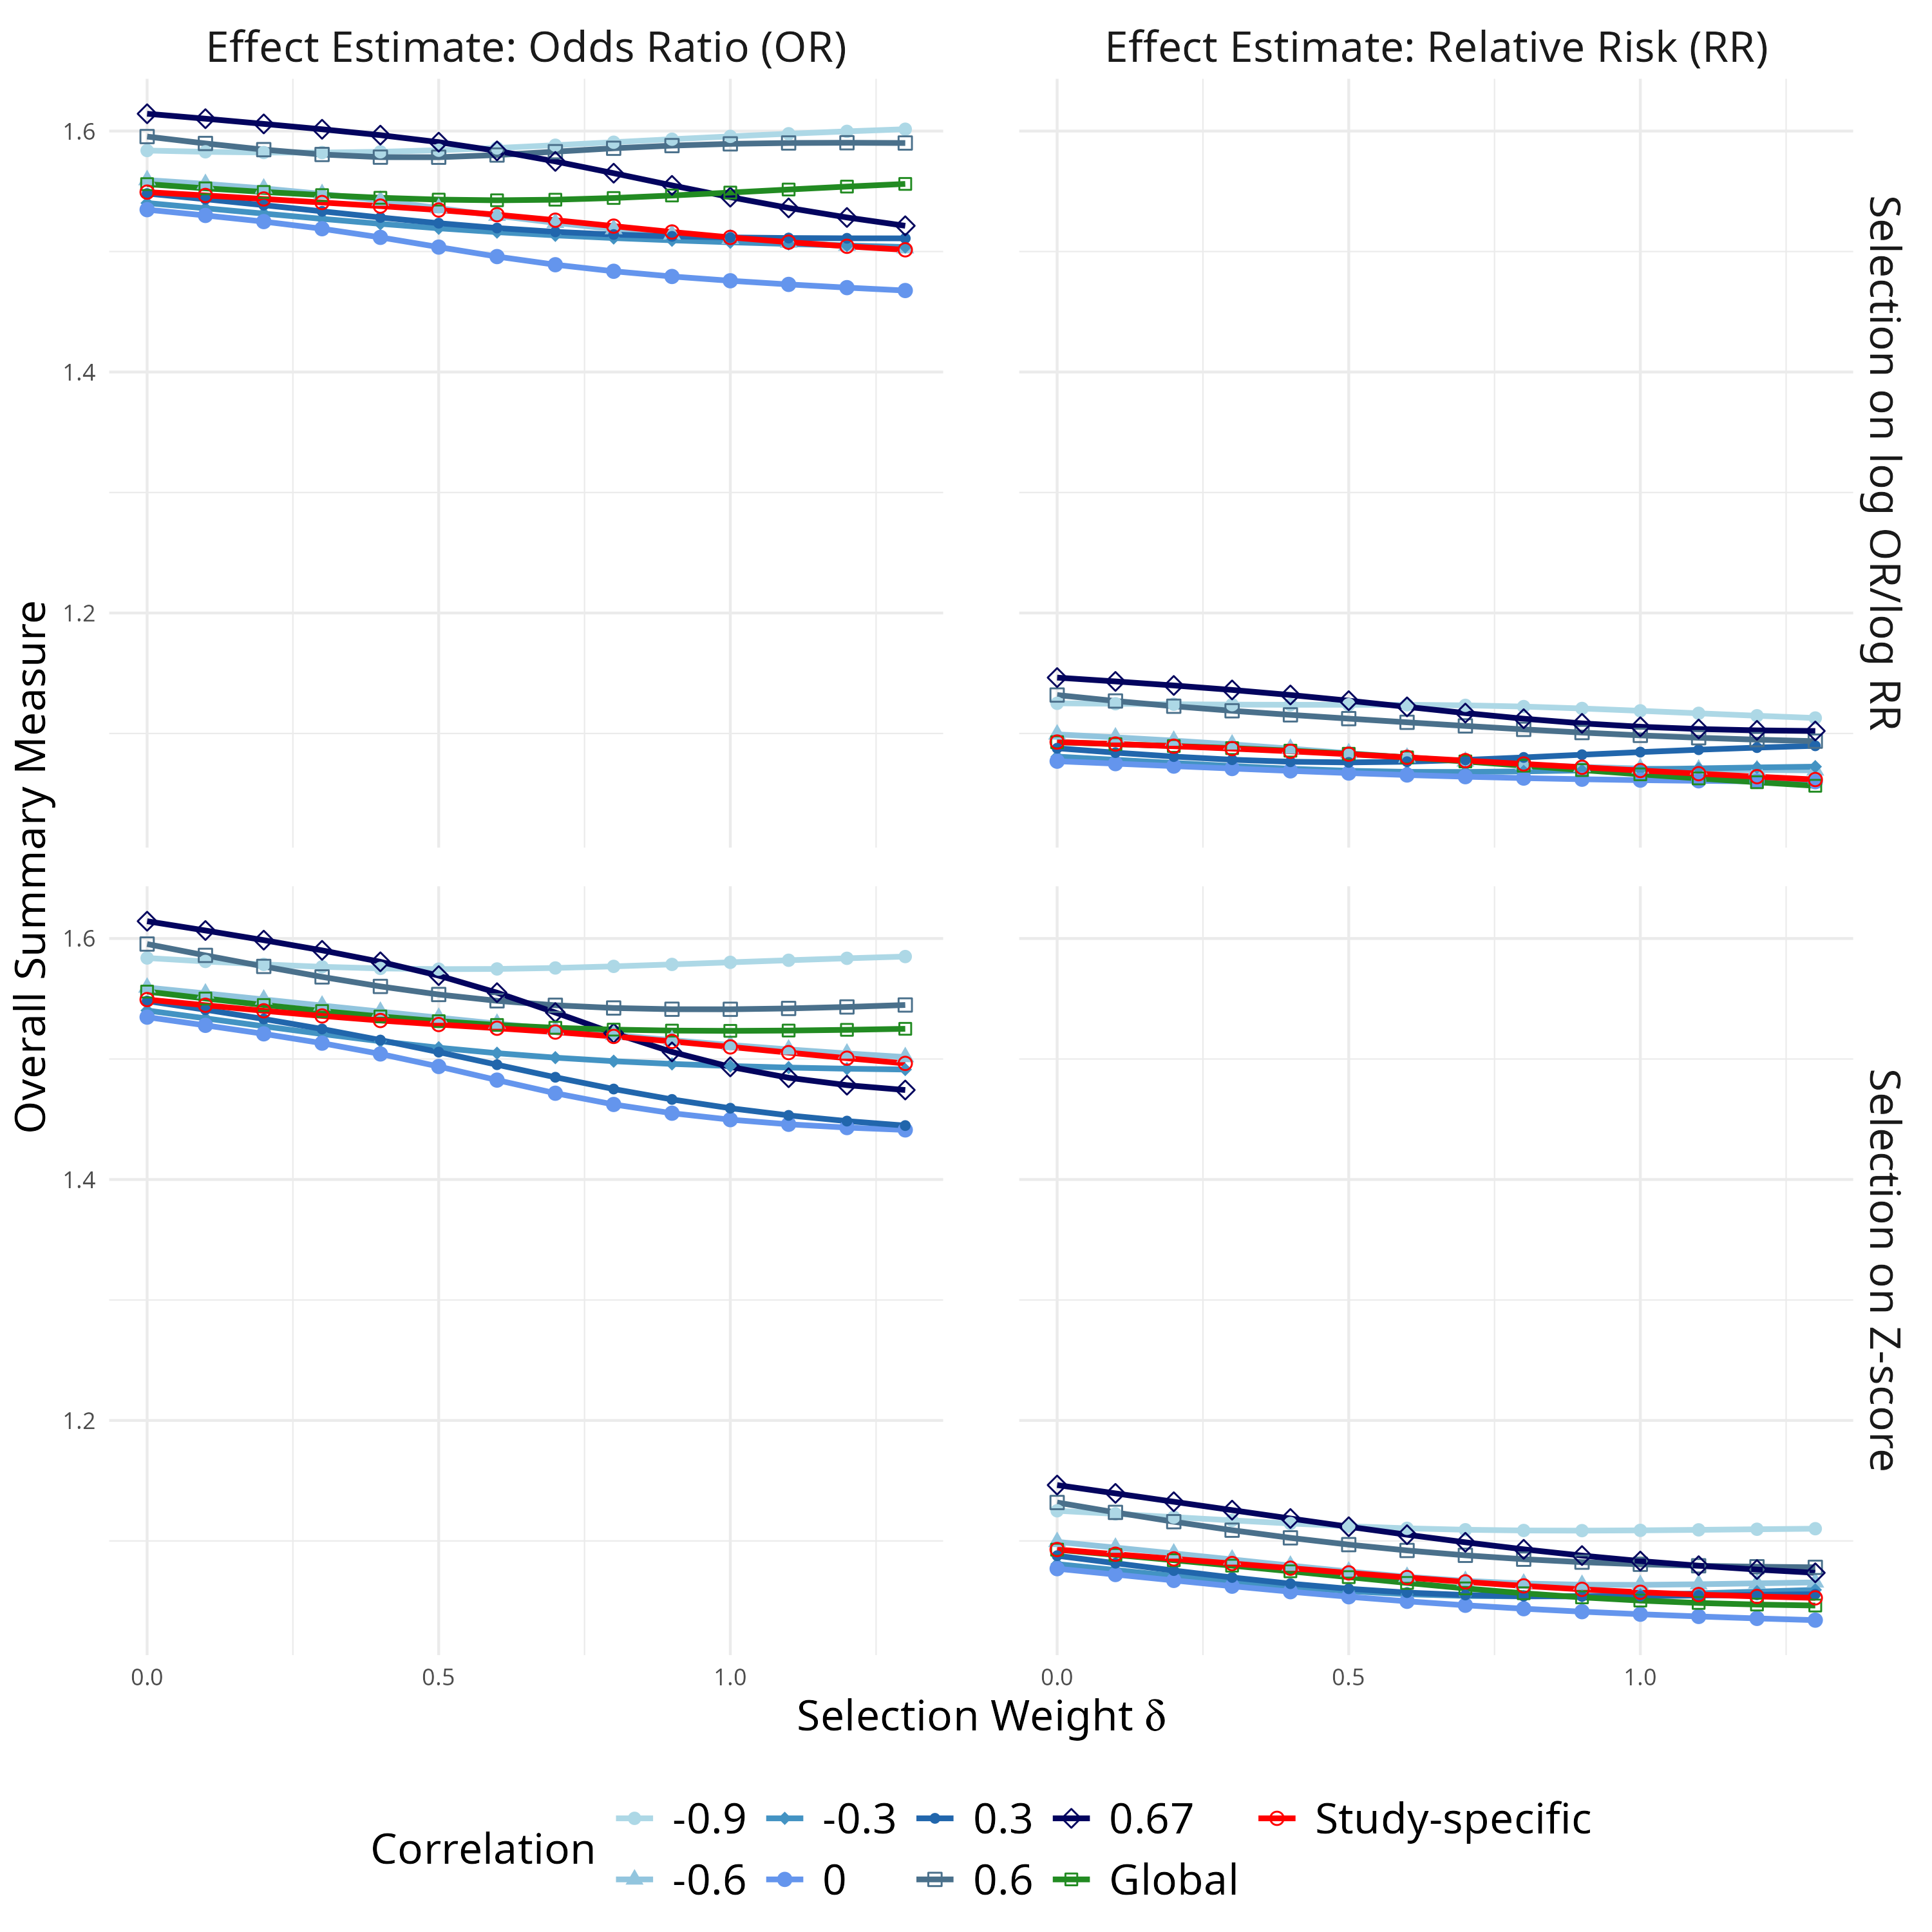
\includegraphics[width = 1\linewidth]{figures/App_Corr_12_mv_REM_O1.png}
\end{figure}

Figure \ref{fig:Multivariate2} compares the three approaches for incorporating within-study correlation for the outcome \textit{50\% seizure reduction}. In contrast to \textit{seizure freedom}, only a single study outcome is unreported for this outcome. Consequently, the adjusted estimates are only weakly affected by the assumed within-study correlation, and the curves remain closely clustered across the full range of selection parameters. Differences between correlation assumptions are already present at $\delta = 0$, reflecting the influence of the covariance structure on the imputed value under MAR. As the selection parameter increases, the adjusted estimates change only modestly because the overall analysis is driven primarily by the reported outcomes. The study-specific correlation reflects the additional variability introduced by sampling a separate correlation for each study, although the overall differences remain small.

Overall, the results for \textit{50\% seizure reduction} demonstrate that the magnitude and stability of ORB adjustment depends strongly on the proportion of unreported study outcomes. When only a small proportion of outcomes is unreported, both univariate and multivariate adjustments remain relatively modest and robust to different modeling assumptions. In contrast, outcomes with a larger proportion of missing information are substantially more sensitive to assumptions regarding the selection type and the within-study correlation structure. These findings highlight that multivariate ORB adjustment is most influential in settings with substantial selective non-reporting, where borrowing strength across correlated outcomes can alter the adjusted estimates and their uncertainty.

\subsection{\mycolor{Comparison to established ORB-adjustment methods}}

\begin{figure}[!ht]
\centering
\caption{Forest plot for comparison of ORB-adjustment methods applied to the outcome \textit{50\% seizure reduction} of the Topiramate data. For the bivariate analyses, the within-study correlation is estimated with the Pearson correlation.
\textit{Notes:} (1) and (2) denote the two piecewise-decreasing selection functions considered by Saracini and Held: (1) $\gamma = 7, \beta = 1.5$, (2) $\gamma = 1.5, \beta = 7$. FE stands for fixed-effect.}
\label{fig:Forestplot_Comparison_O1.png}
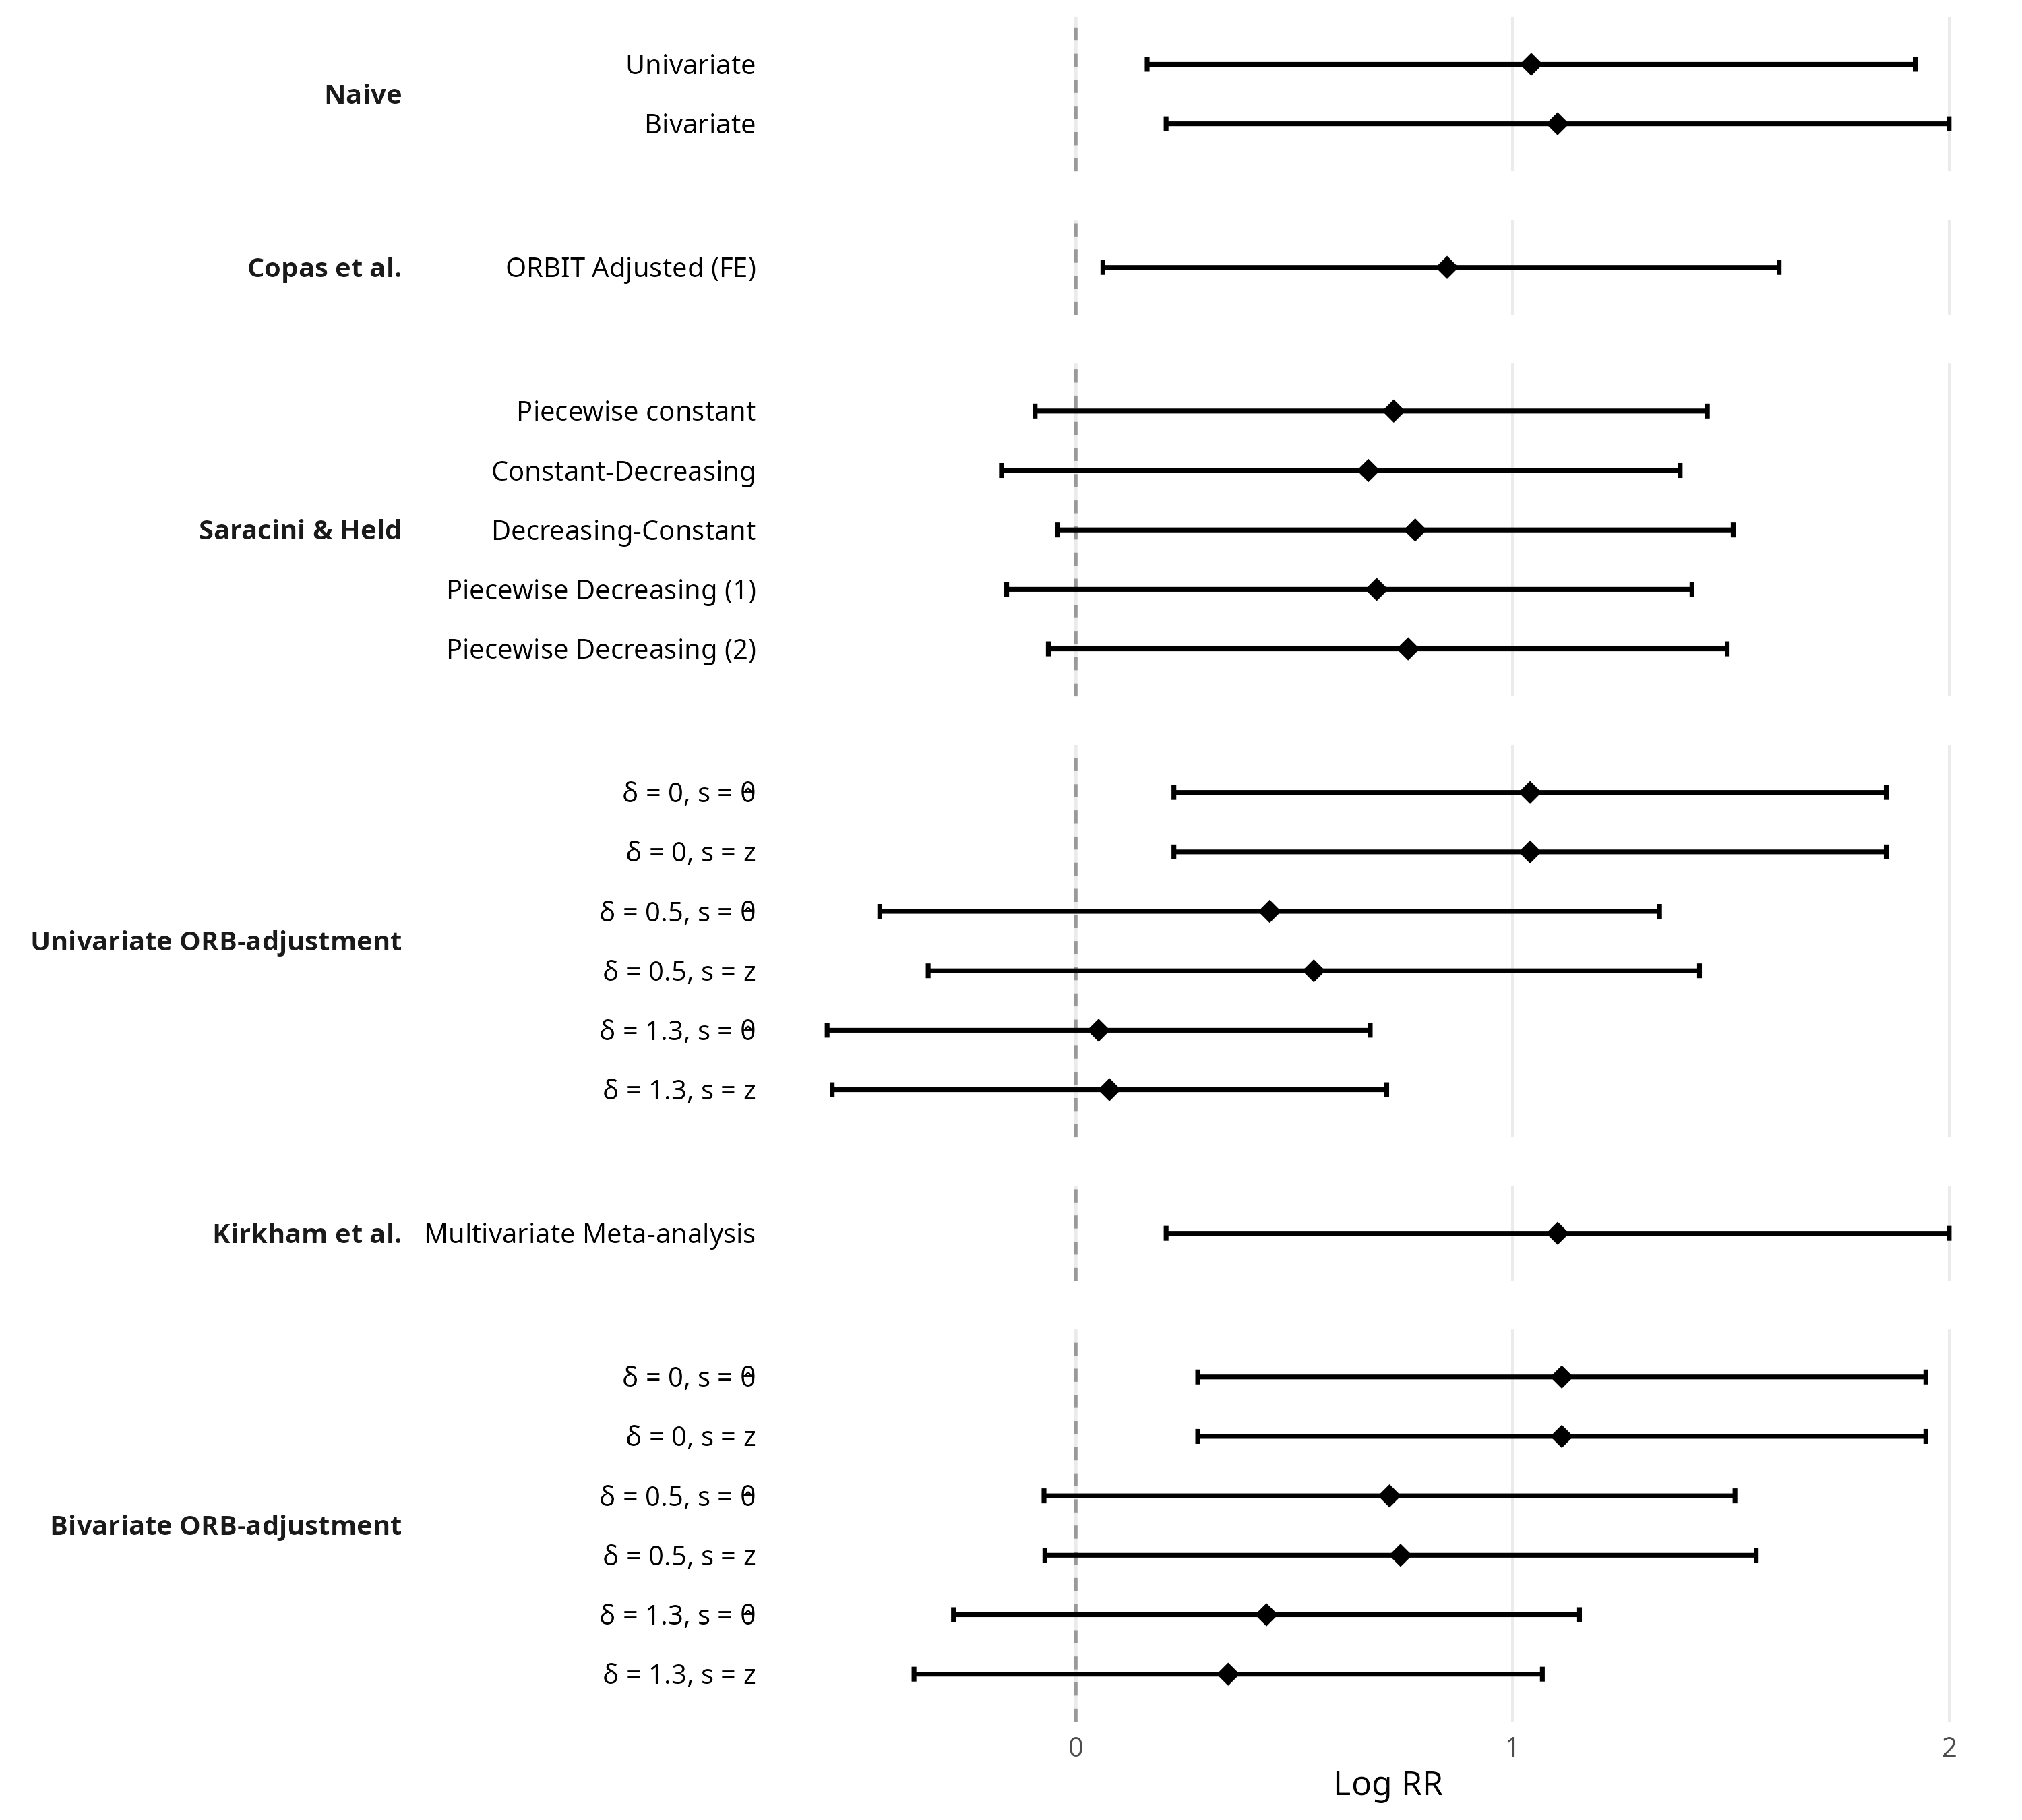
\includegraphics[width = 1\linewidth]{figures/Forestplot_Comparison_O1.png}
\end{figure}

\mycolor{Figure \ref{fig:Forestplot_Comparison_O1.png} compares our univariate and bivariate ORB-adjustment method to established approaches that account for ORB for the outcome \textit{50\% seizure reduction}. For the univariate adjustment, we compared our approach for three different selection parameters to Copas sensitivity analyis based on the ORBIT classification \cite{copas2019model} and to the selection models proposed by Saracini and Held \cite{saracini2025addressing}. The Copas model is the only fixed-effect approach shown, the other approaches shown are based on REMs. Despite differences in their underlying assumptions and model specifications, the methods generally point in the same direction. The Copas, Saracini and Held and our univariate ORB-adjustment approaches yield estimates in a similar range, with the Copas estimate showing the strongest adjustment. For the bivariate case, we only compared our approach to that of Kirkham et al. \cite{kirkham2012multivariate}, which is essentially equivalent to that obtained from the bivariate REM without ORB adjustment. For both the univariate and bivariate ORB-adjustment approaches, increasing the selection parameter $\delta$ leads to slightly smaller estimates. Since for \textit{seizure reduction} only one study outcome out of twelve is unreported one can see only slight differences between the naive estimates and the adjusted estimates in comparison to \textit{seizure freedom} for which six out of twelve are unreported (see Figure \ref{fig:Forestplot_Comparison_O2.png}).}

\subsection{\mycolor{Sensitivity analysis for reduction in the number of imputations}}

\mycolor{To check that the reduction in the number of imputations does not change the results, the bivariate adjustment was applied to the topiramate data with $M = 1000$ imputations and the adjusted estimate recomputed from the first 200 of them, on the log OR and the log RR scale. The within-study correlation was fixed at $\rho_W = -0.3$ (the estimated Pearson correlation), while the between-study variances and correlation were estimated. Both outcomes were considered, \textit{50\% seizure reduction} (one study unreported) and \textit{seizure freedom} (six of twelve studies unreported), with selection on the $z$-score and on the effect estimate, for $\delta$ from 0 to 1.3.}

\begin{figure}[ht!]
\centering
\caption{Adjusted estimate (line) and 95\% CI (band) as a function of the selection parameter $\delta$, computed from $M = 200$ (orange) and from $M = 1000$ (blue) imputations of the same analysis.}
\label{fig:App_M_convergence}
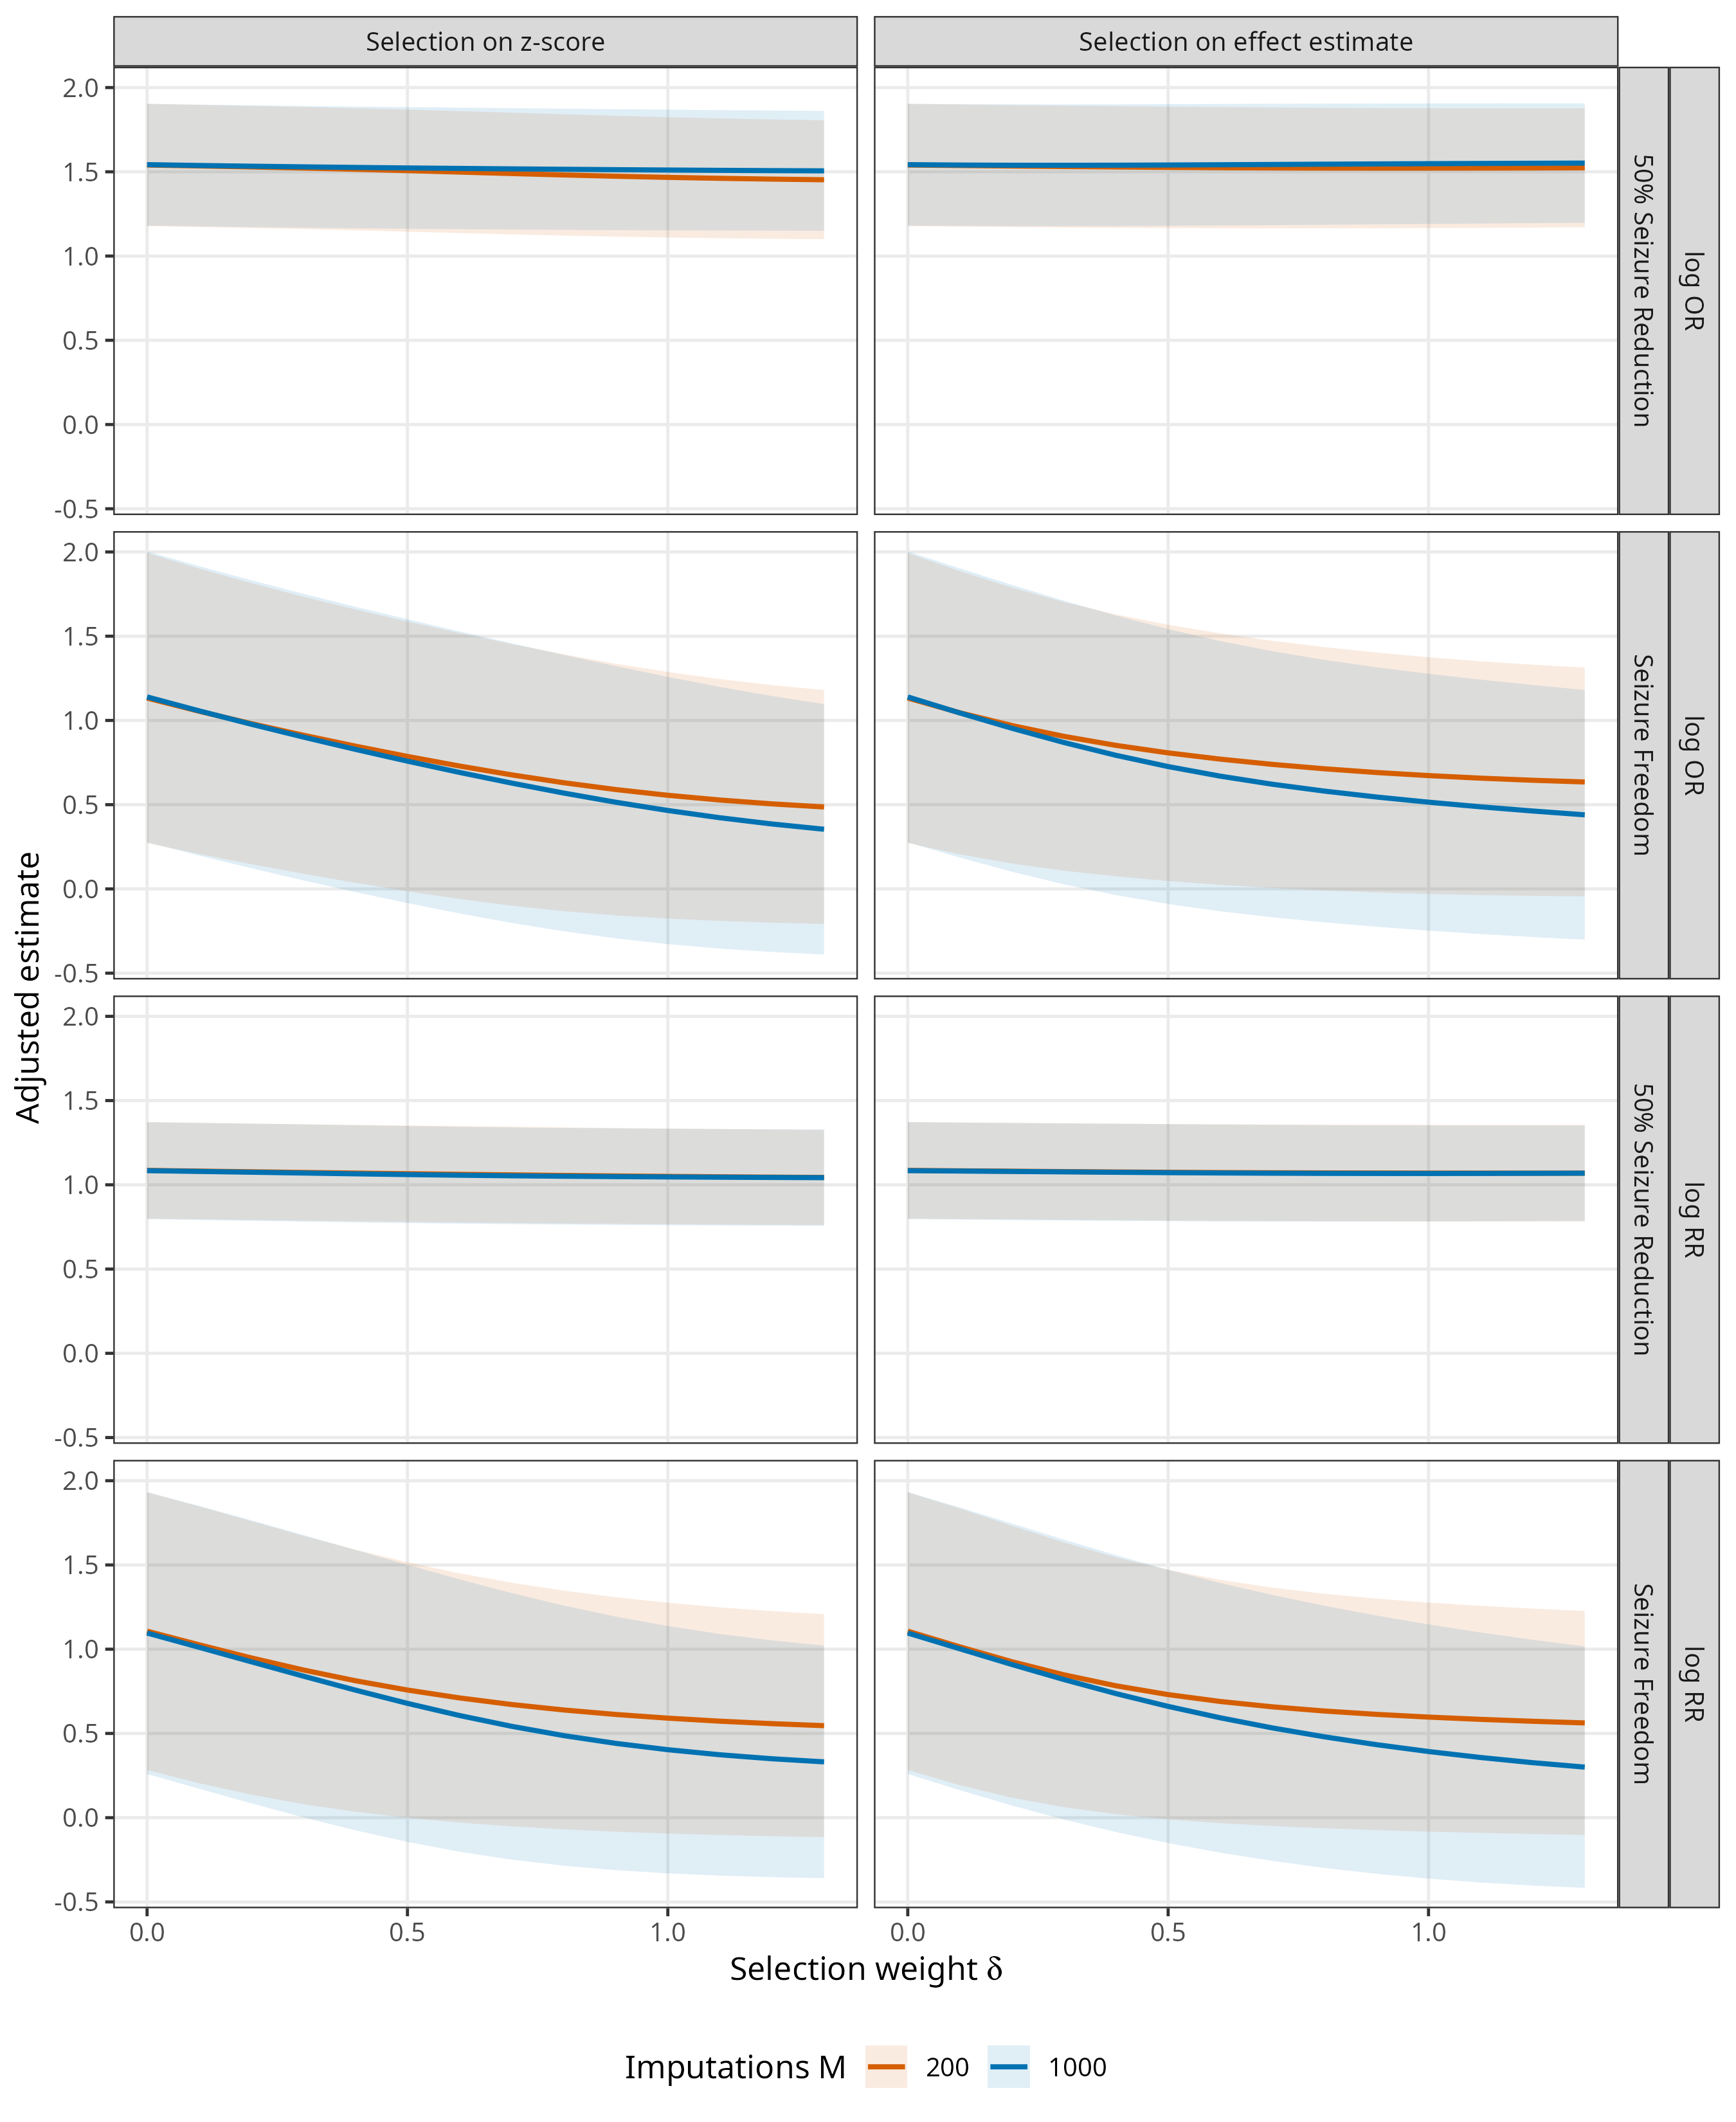
\includegraphics[width = 1\linewidth]{figures/App_M_convergence.png}
\end{figure}
\noindent
\mycolor{For \textit{50\% seizure reduction} the two curves coincide on both scales (largest difference 0.06, against CIs about 0.6 to 0.7 wide). For \textit{seizure freedom} they overlap up to $\delta = 0.5$ and differ by at most 0.12 at larger delta, well within CIs 1.3 to 1.8 wide. $M = 200$ therefore leads to the same conclusions as $M = 1000$.}

\clearpage
\section{Simulation Study}

\subsection{\mycolor{Repetion-wise deletion for main scenario}}
\label{Repetition}
\mycolor{As a sensitvity analysis we also considered reptition-wise deletion where only simulation repetitions for which all methods successfully produced results were retained \cite{pawel2025handling}. Bias, mean squared error, coverage, and CI width were recalculated for all methods using this common set of repetitions. When comparing method-wise deletion (Figure \ref{fig:Bias} - Figure \ref{fig:Coverage}) and repetition-wise deletion for the main scenario, \ie $\theta_1 = \theta_2 = 0.4$, $\rho_B = \rho_W = 0.8$ and $p_1 = 20\%$, one cannot see any differences visually.} 

\begin{figure}[!ht]
\centering
\caption{Simulation results for bias of four MA estimates of the treatment effect for outcome 1 under ORB for $\theta_1 = \theta_2 = 0.4$, $\rho_B = \rho_W = 0.8$ and $p_1 = 20\%$. Results are shown for varying numbers of studies, heterogeneity levels, selection type, and an increasing selection parameter.}
\label{fig:App_Bias_RepDel}
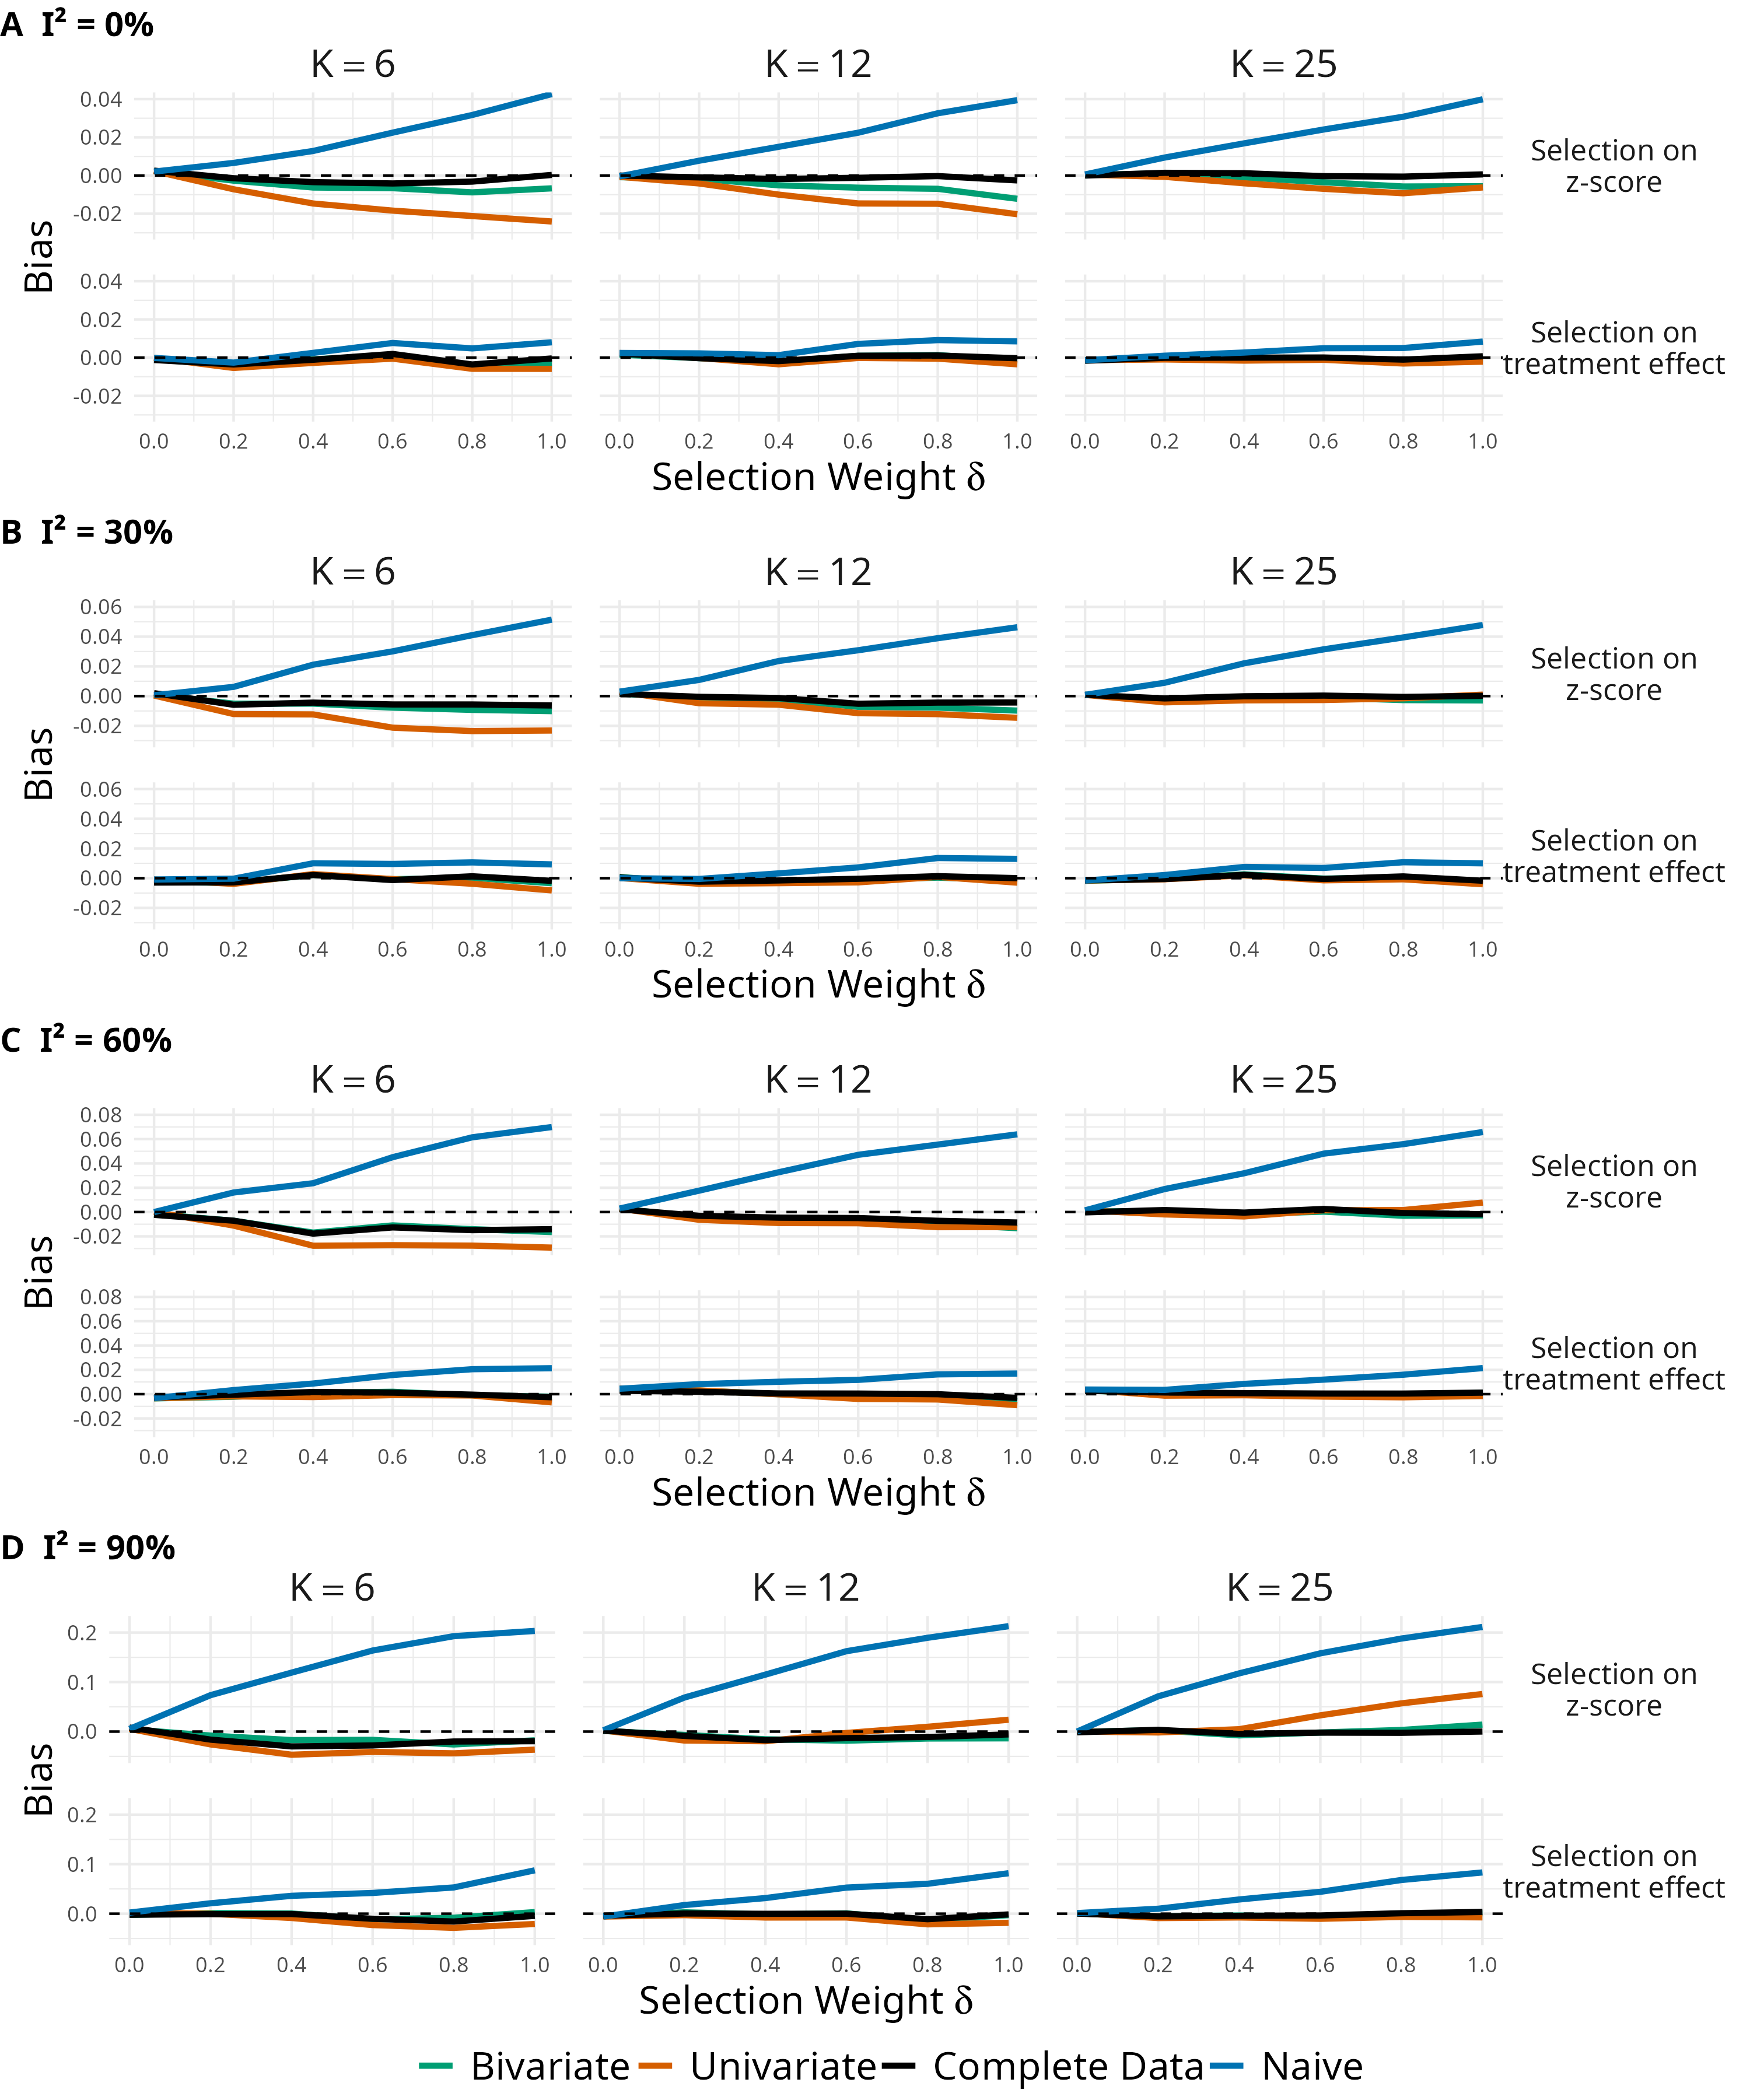
\includegraphics[width = 1\linewidth]{figures/SimStudy_Bias_RepDel.png}
\end{figure}

\mycolor{Because repetition-wise deletion retains only repetitions in which all methods produced valid results, method-specific failure rates are not separately meaningful within this subsample by construction. Instead, we report the overall proportion of eligible repetitions excluded from the repetition-wise analysis due to failure of at least one method. Across all simulated scenarios, the proportion of eligible repetitions excluded due to failure of at least one method was negligible (maximum $0.009\%$, $K = 6$, $I^2=60\%$), with most scenarios showing no exclusions at all. This indicates that method-wise and repetition-wise deletion were applied to essentially identical sets of repetitions, and as result, the performance measures for method-wise deletion and repetition-wise deletion show no differences.}

\begin{figure}[!ht]
\centering
\caption{Simulation results for MSE of four MA estimates of the treatment effect for outcome 1 under ORB for $\theta_1 = \theta_2 = 0.4$, $\rho_B = \rho_W = 0.8$ and $p_1 = 20\%$. Results are shown for varying numbers of studies, heterogeneity levels, selection type, and an increasing selection parameter.}
\label{fig:App_MSE_RepDel}
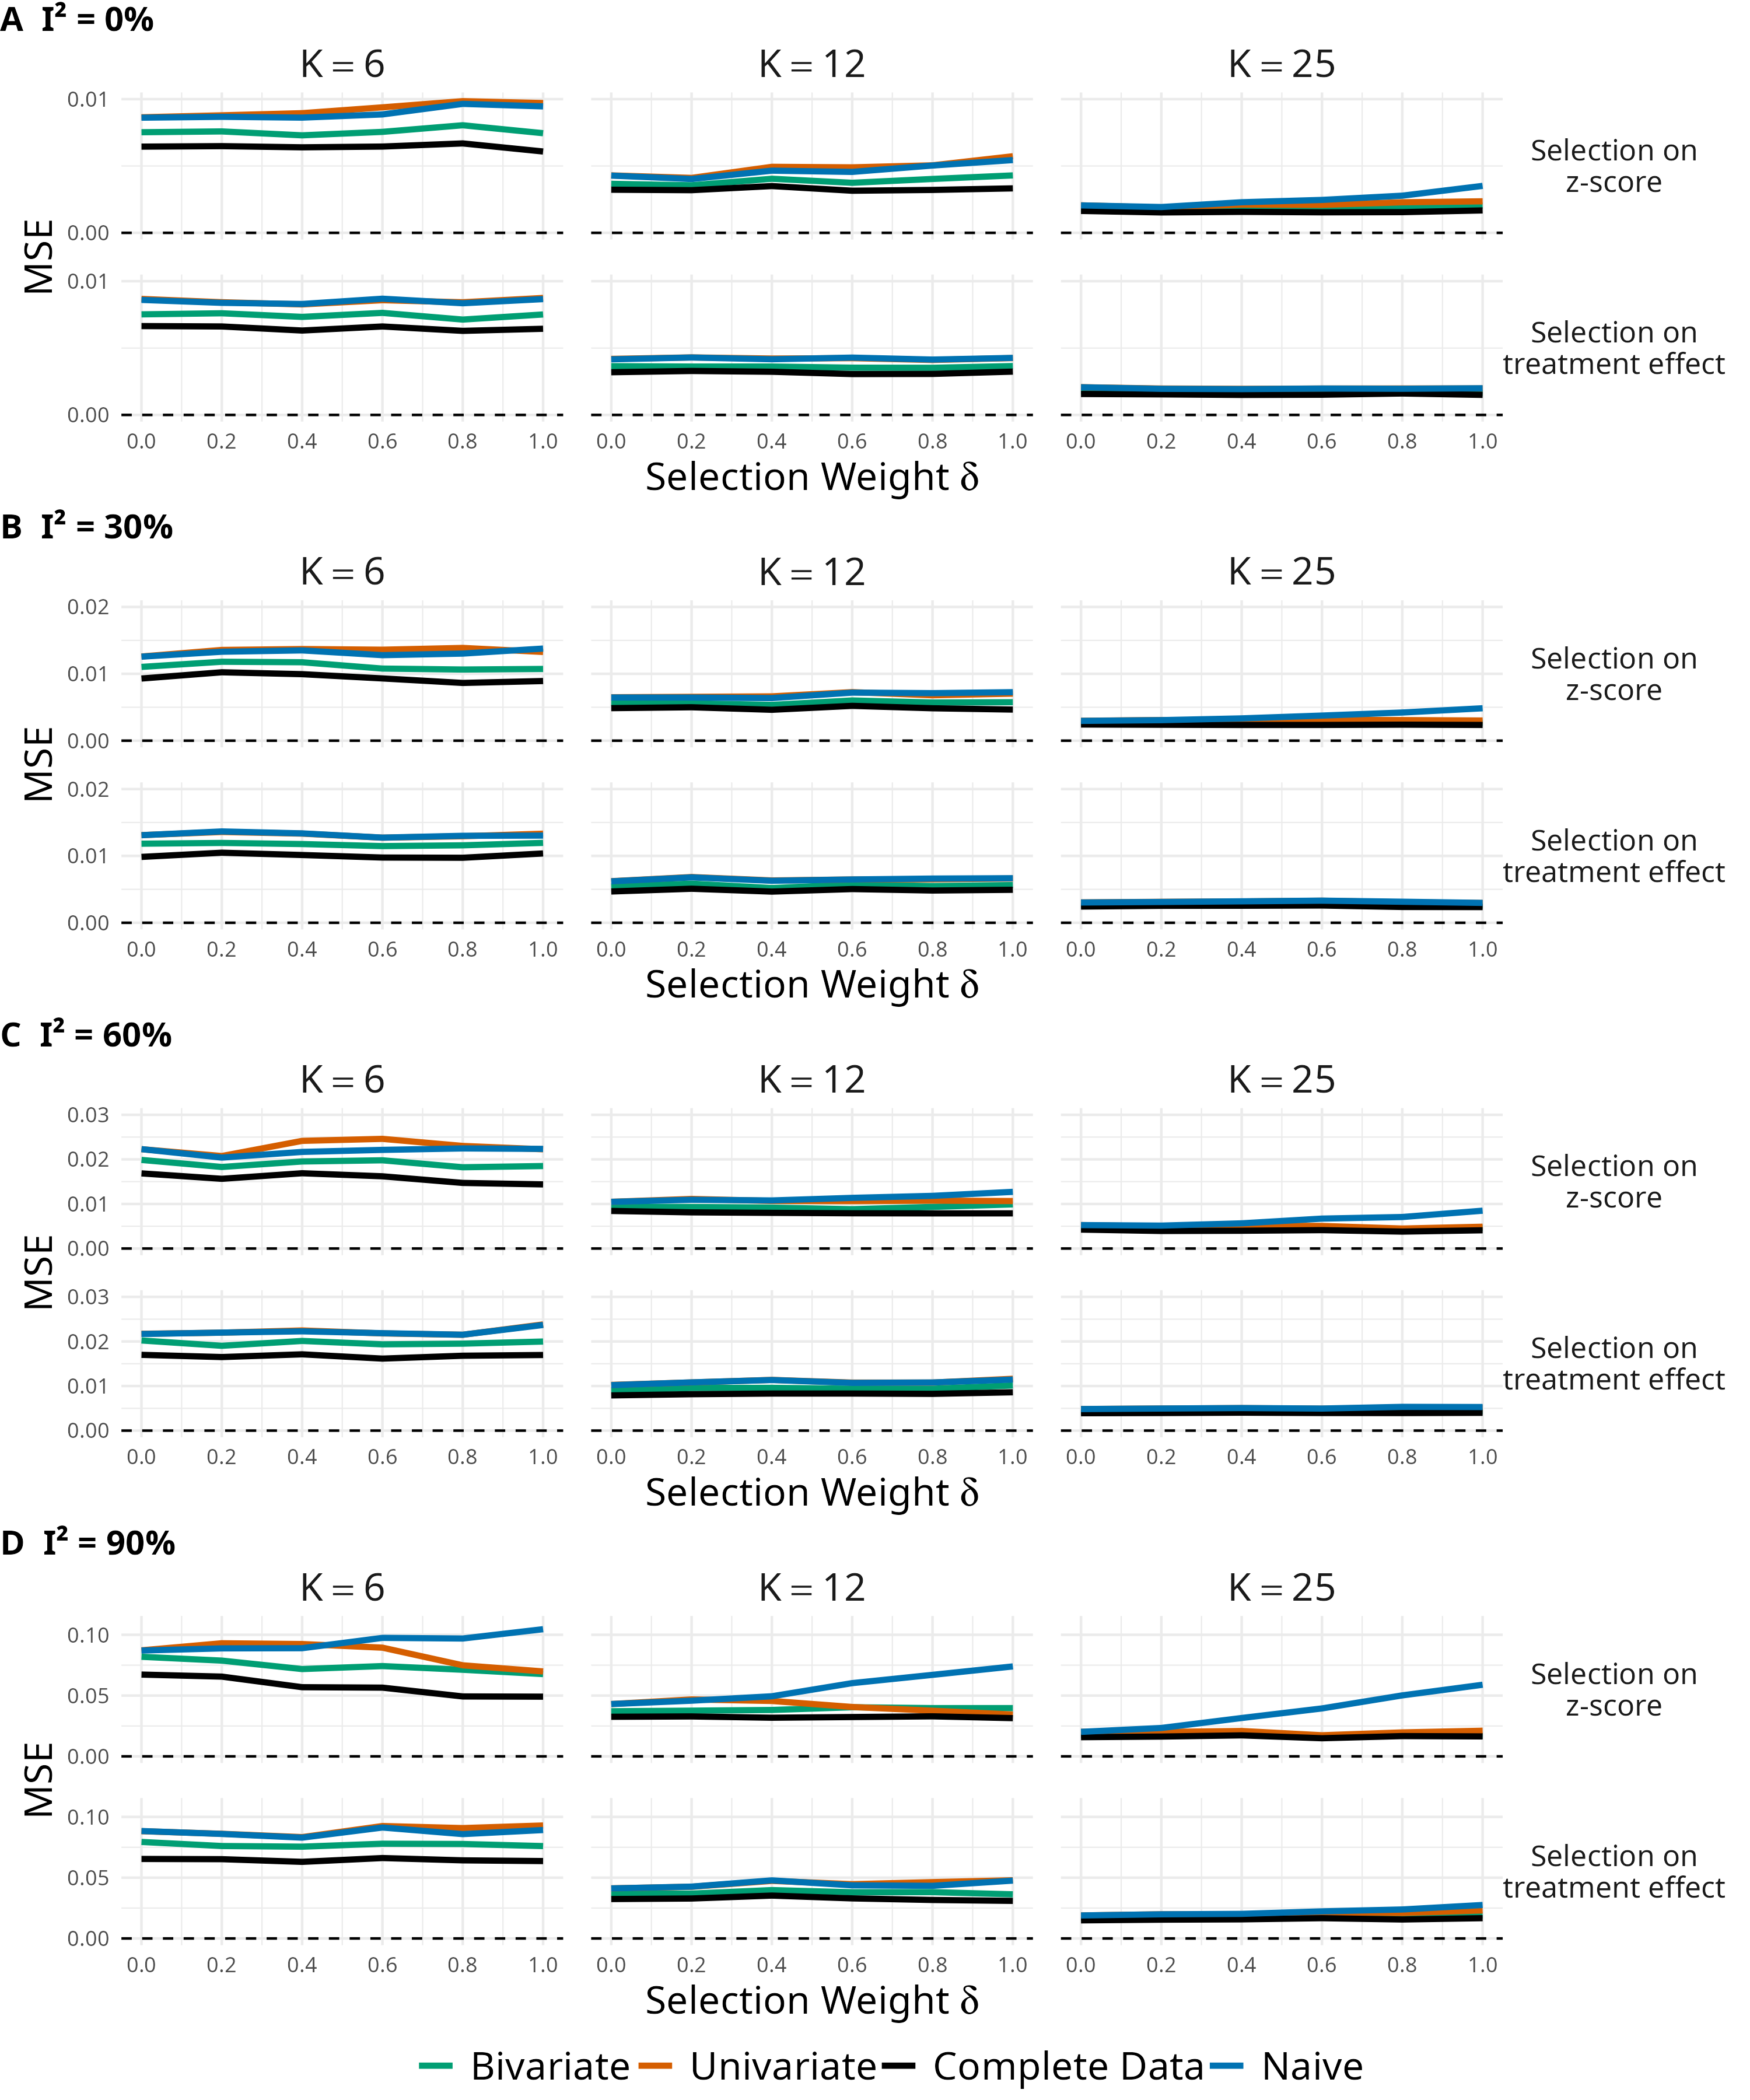
\includegraphics[width = 1\linewidth]{figures/SimStudy_MSE_RepDel.png}
\end{figure}

\begin{figure}[!ht]
\centering
\caption{Simulation results for CI width of four MA estimates of the treatment effect for outcome 1 under ORB for $\theta_1 = \theta_2 = 0.4$, $\rho_B = \rho_W = 0.8$ and $p_1 = 20\%$. Results are shown for varying numbers of studies, heterogeneity levels, selection type, and an increasing selection parameter.}
\label{fig:App_CIWidth_RepDel}
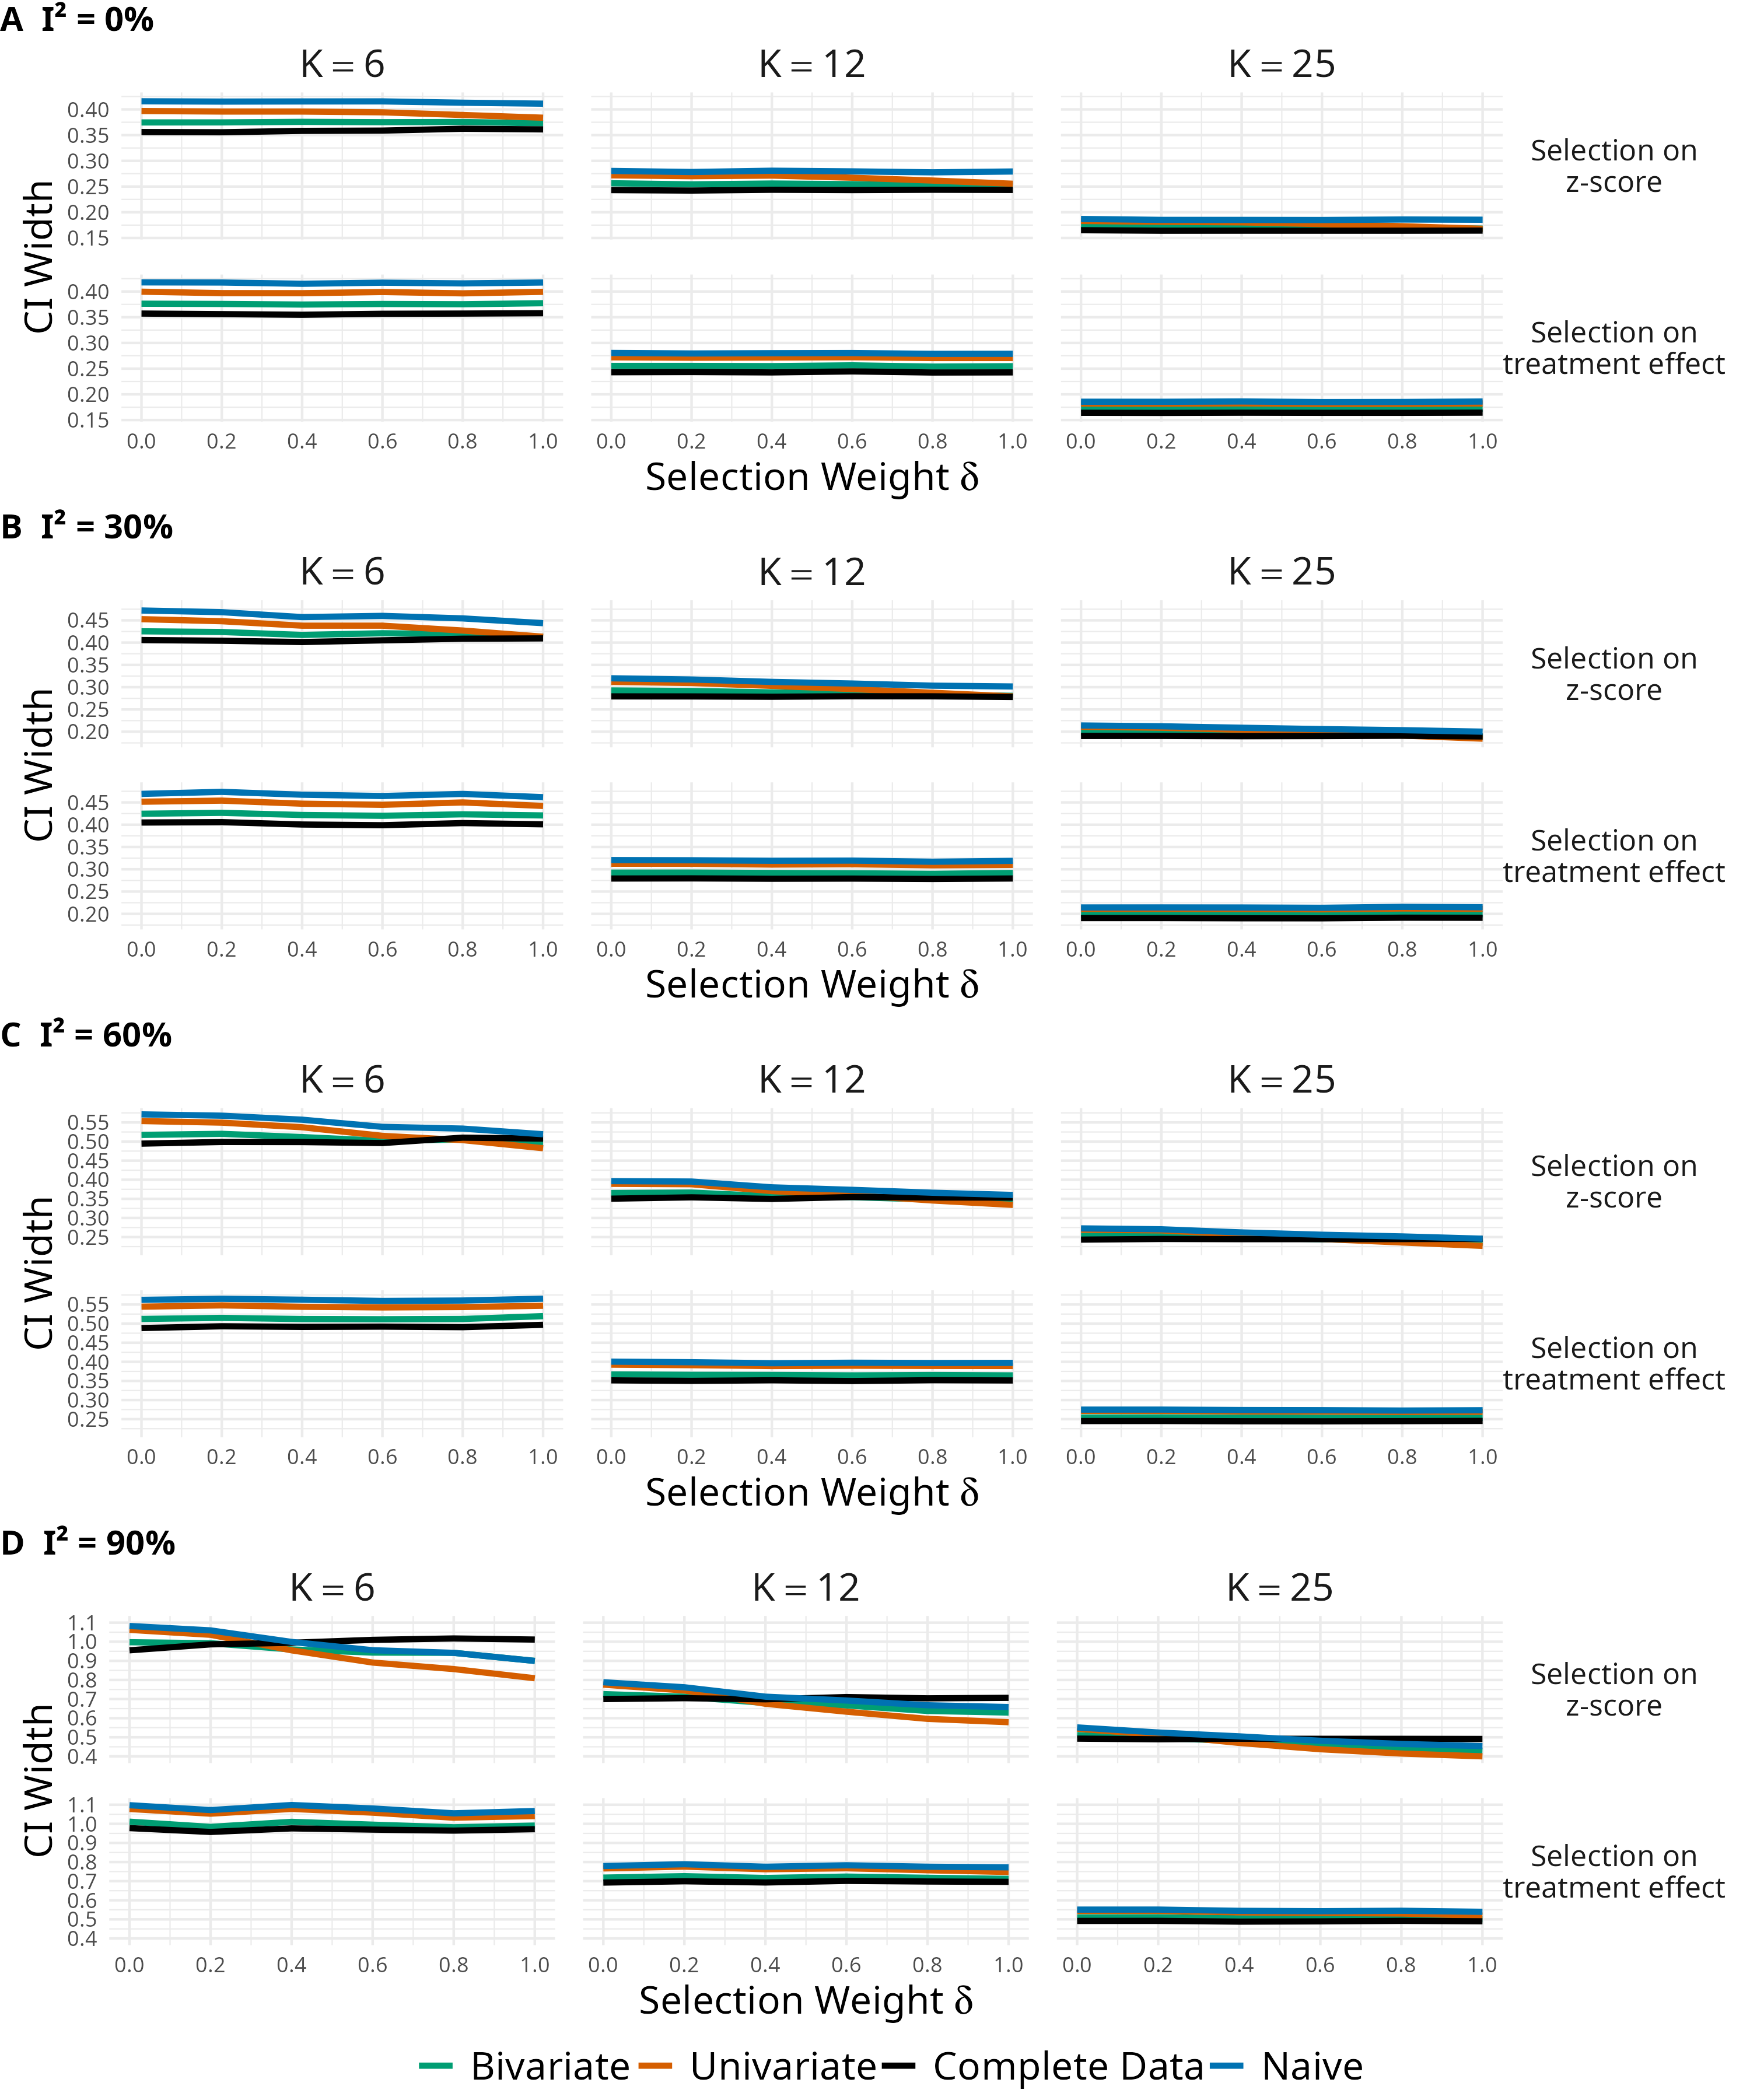
\includegraphics[width = 1\linewidth]{figures/SimStudy_CIWidth_RepDel.png}
\end{figure}

\begin{figure}[!ht]
\centering
\caption{Simulation results for coverage of four MA estimates of the treatment effect for outcome 1 under ORB for $\theta_1 = \theta_2 = 0.4$, $\rho_B = \rho_W = 0.8$ and $p_1 = 20\%$. Results are shown for varying numbers of studies, heterogeneity levels, selection type, and an increasing selection parameter.}
\label{fig:App_Coverage_RepDel}
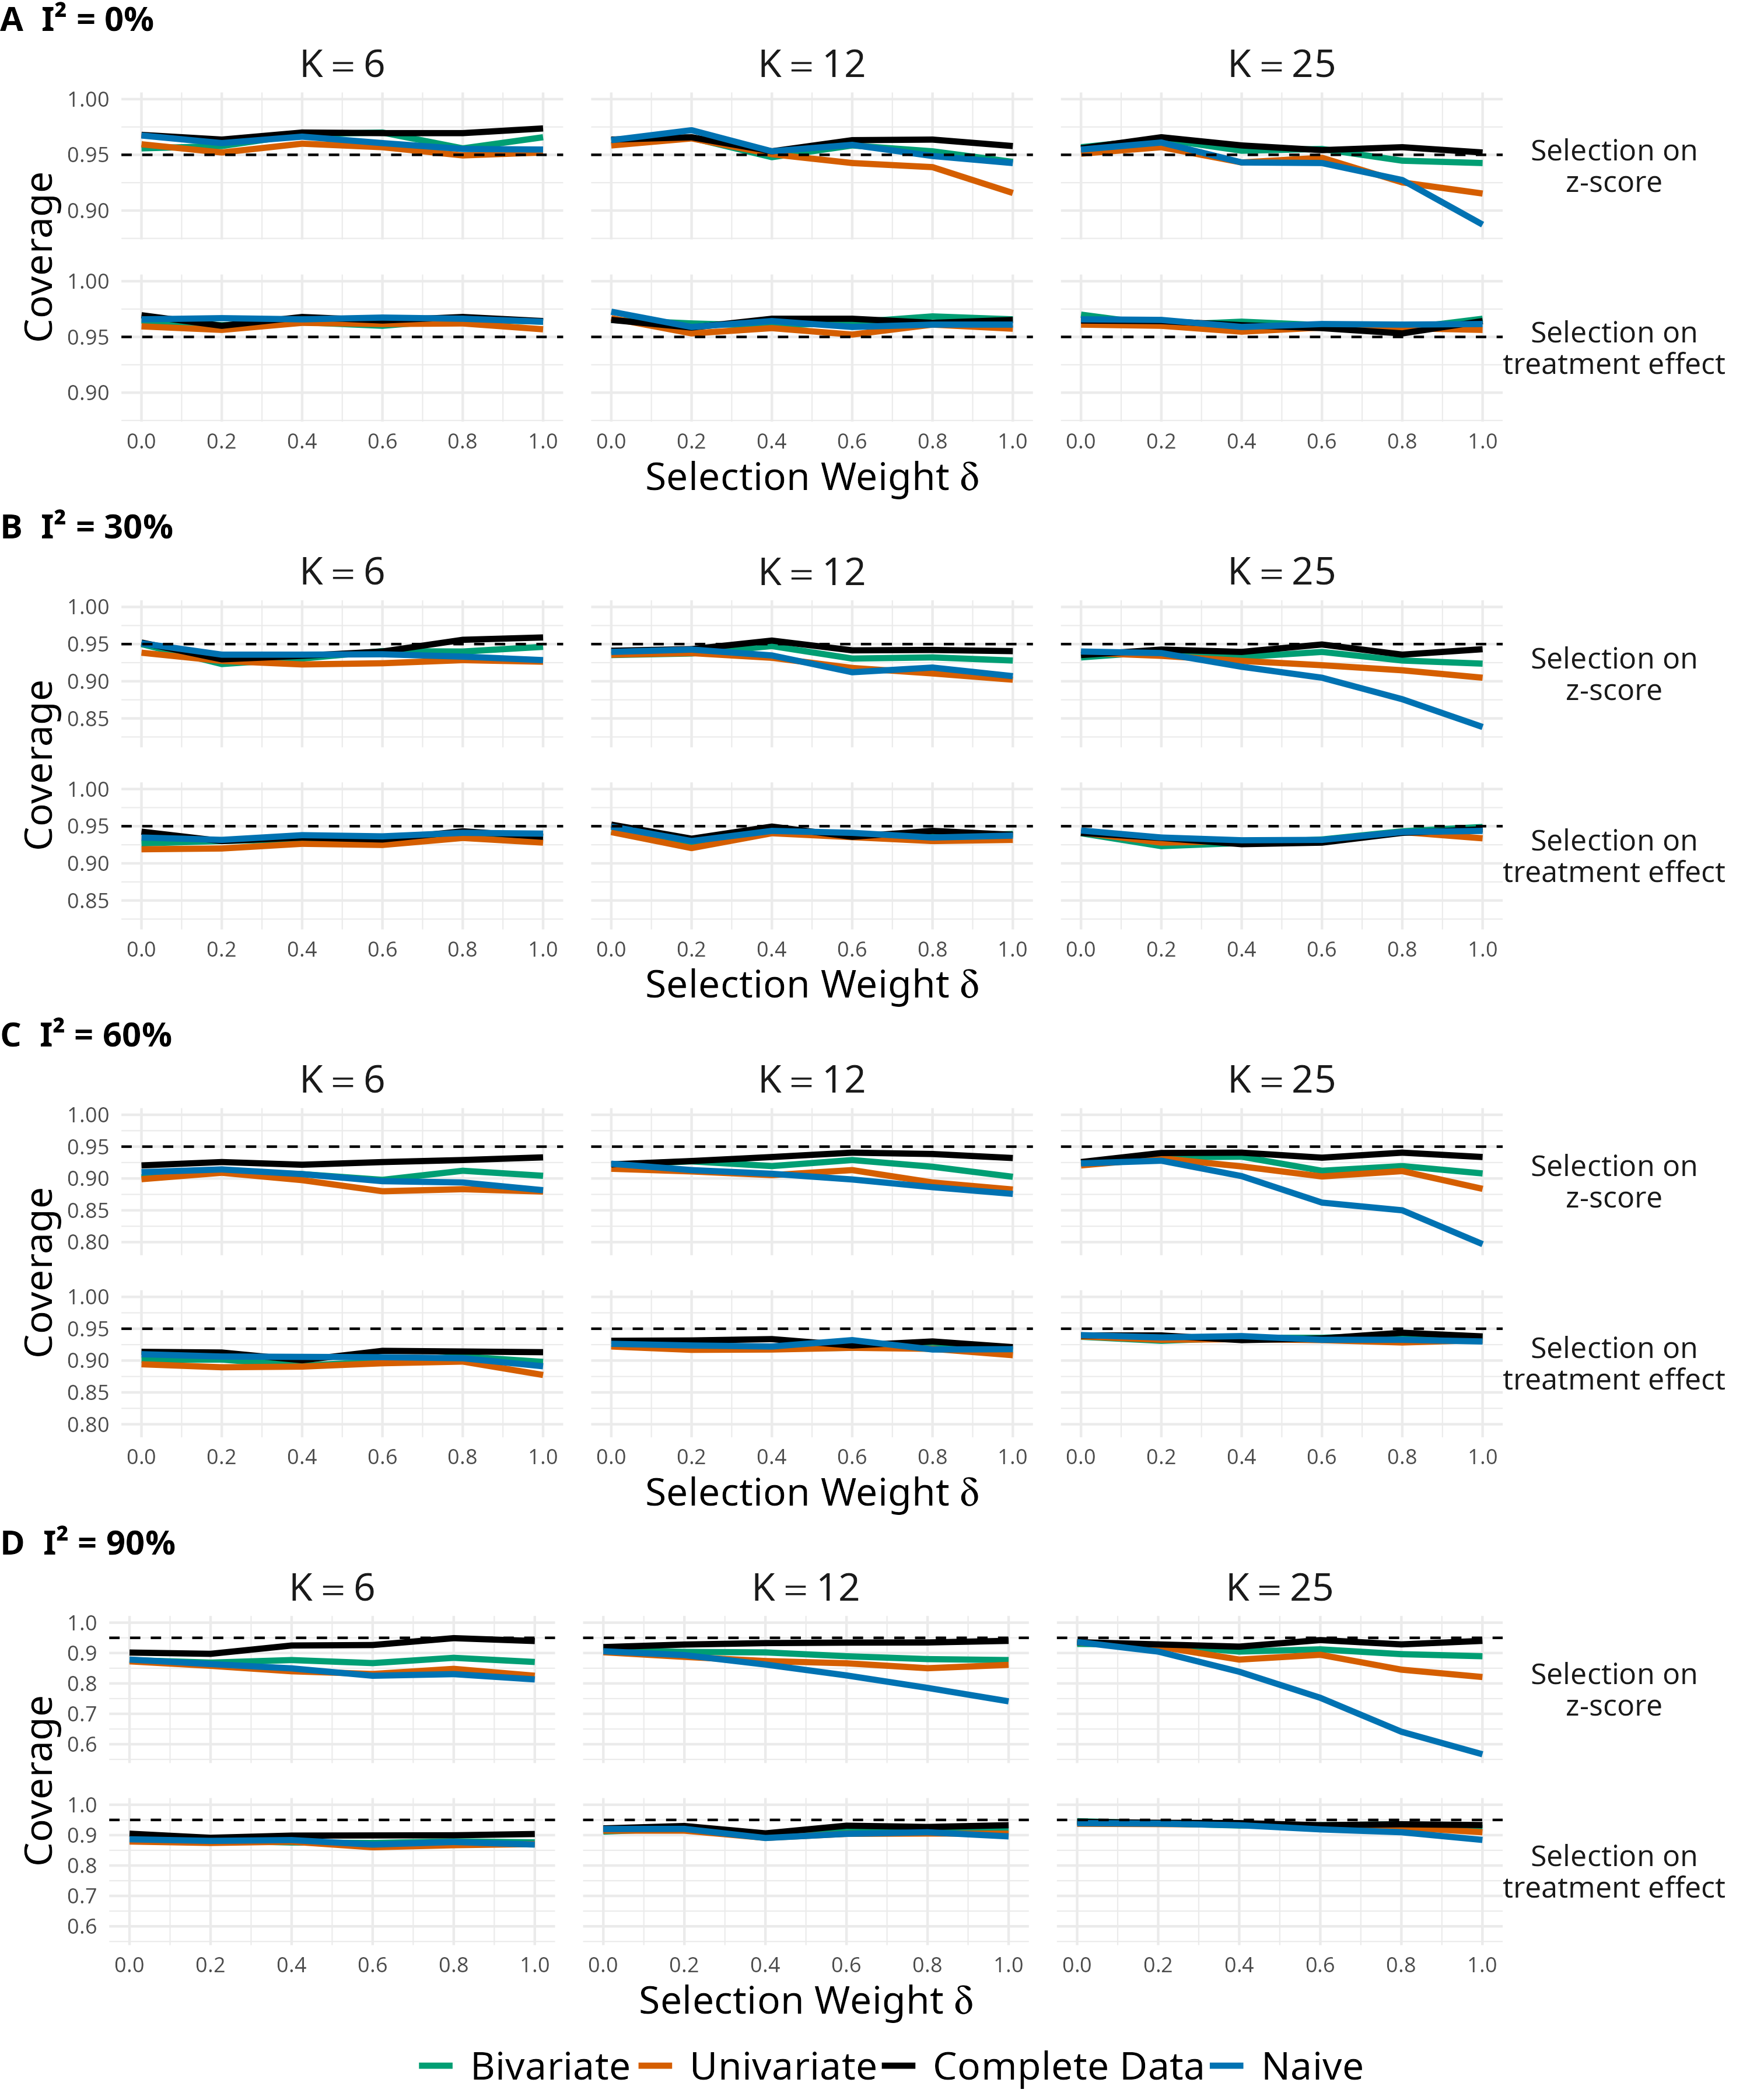
\includegraphics[width = 1\linewidth]{figures/SimStudy_Coverage_RepDel.png}
\end{figure}

\clearpage

\subsection{\mycolor{Proportion of missingness $p_1 = 40\%$ for main scenario}}

\begin{figure}[!ht]
\centering
\caption{Simulation results for bias of four MA estimates of the treatment effect for outcome 1 under ORB for $\theta_1 = \theta_2 = 0.4$, $\rho_B = \rho_W = 0.8$ and $p_1 = 40\%$. Results are shown for varying numbers of studies, heterogeneity levels, selection type, and an increasing selection parameter.}
\label{fig:App_Bias_p04}
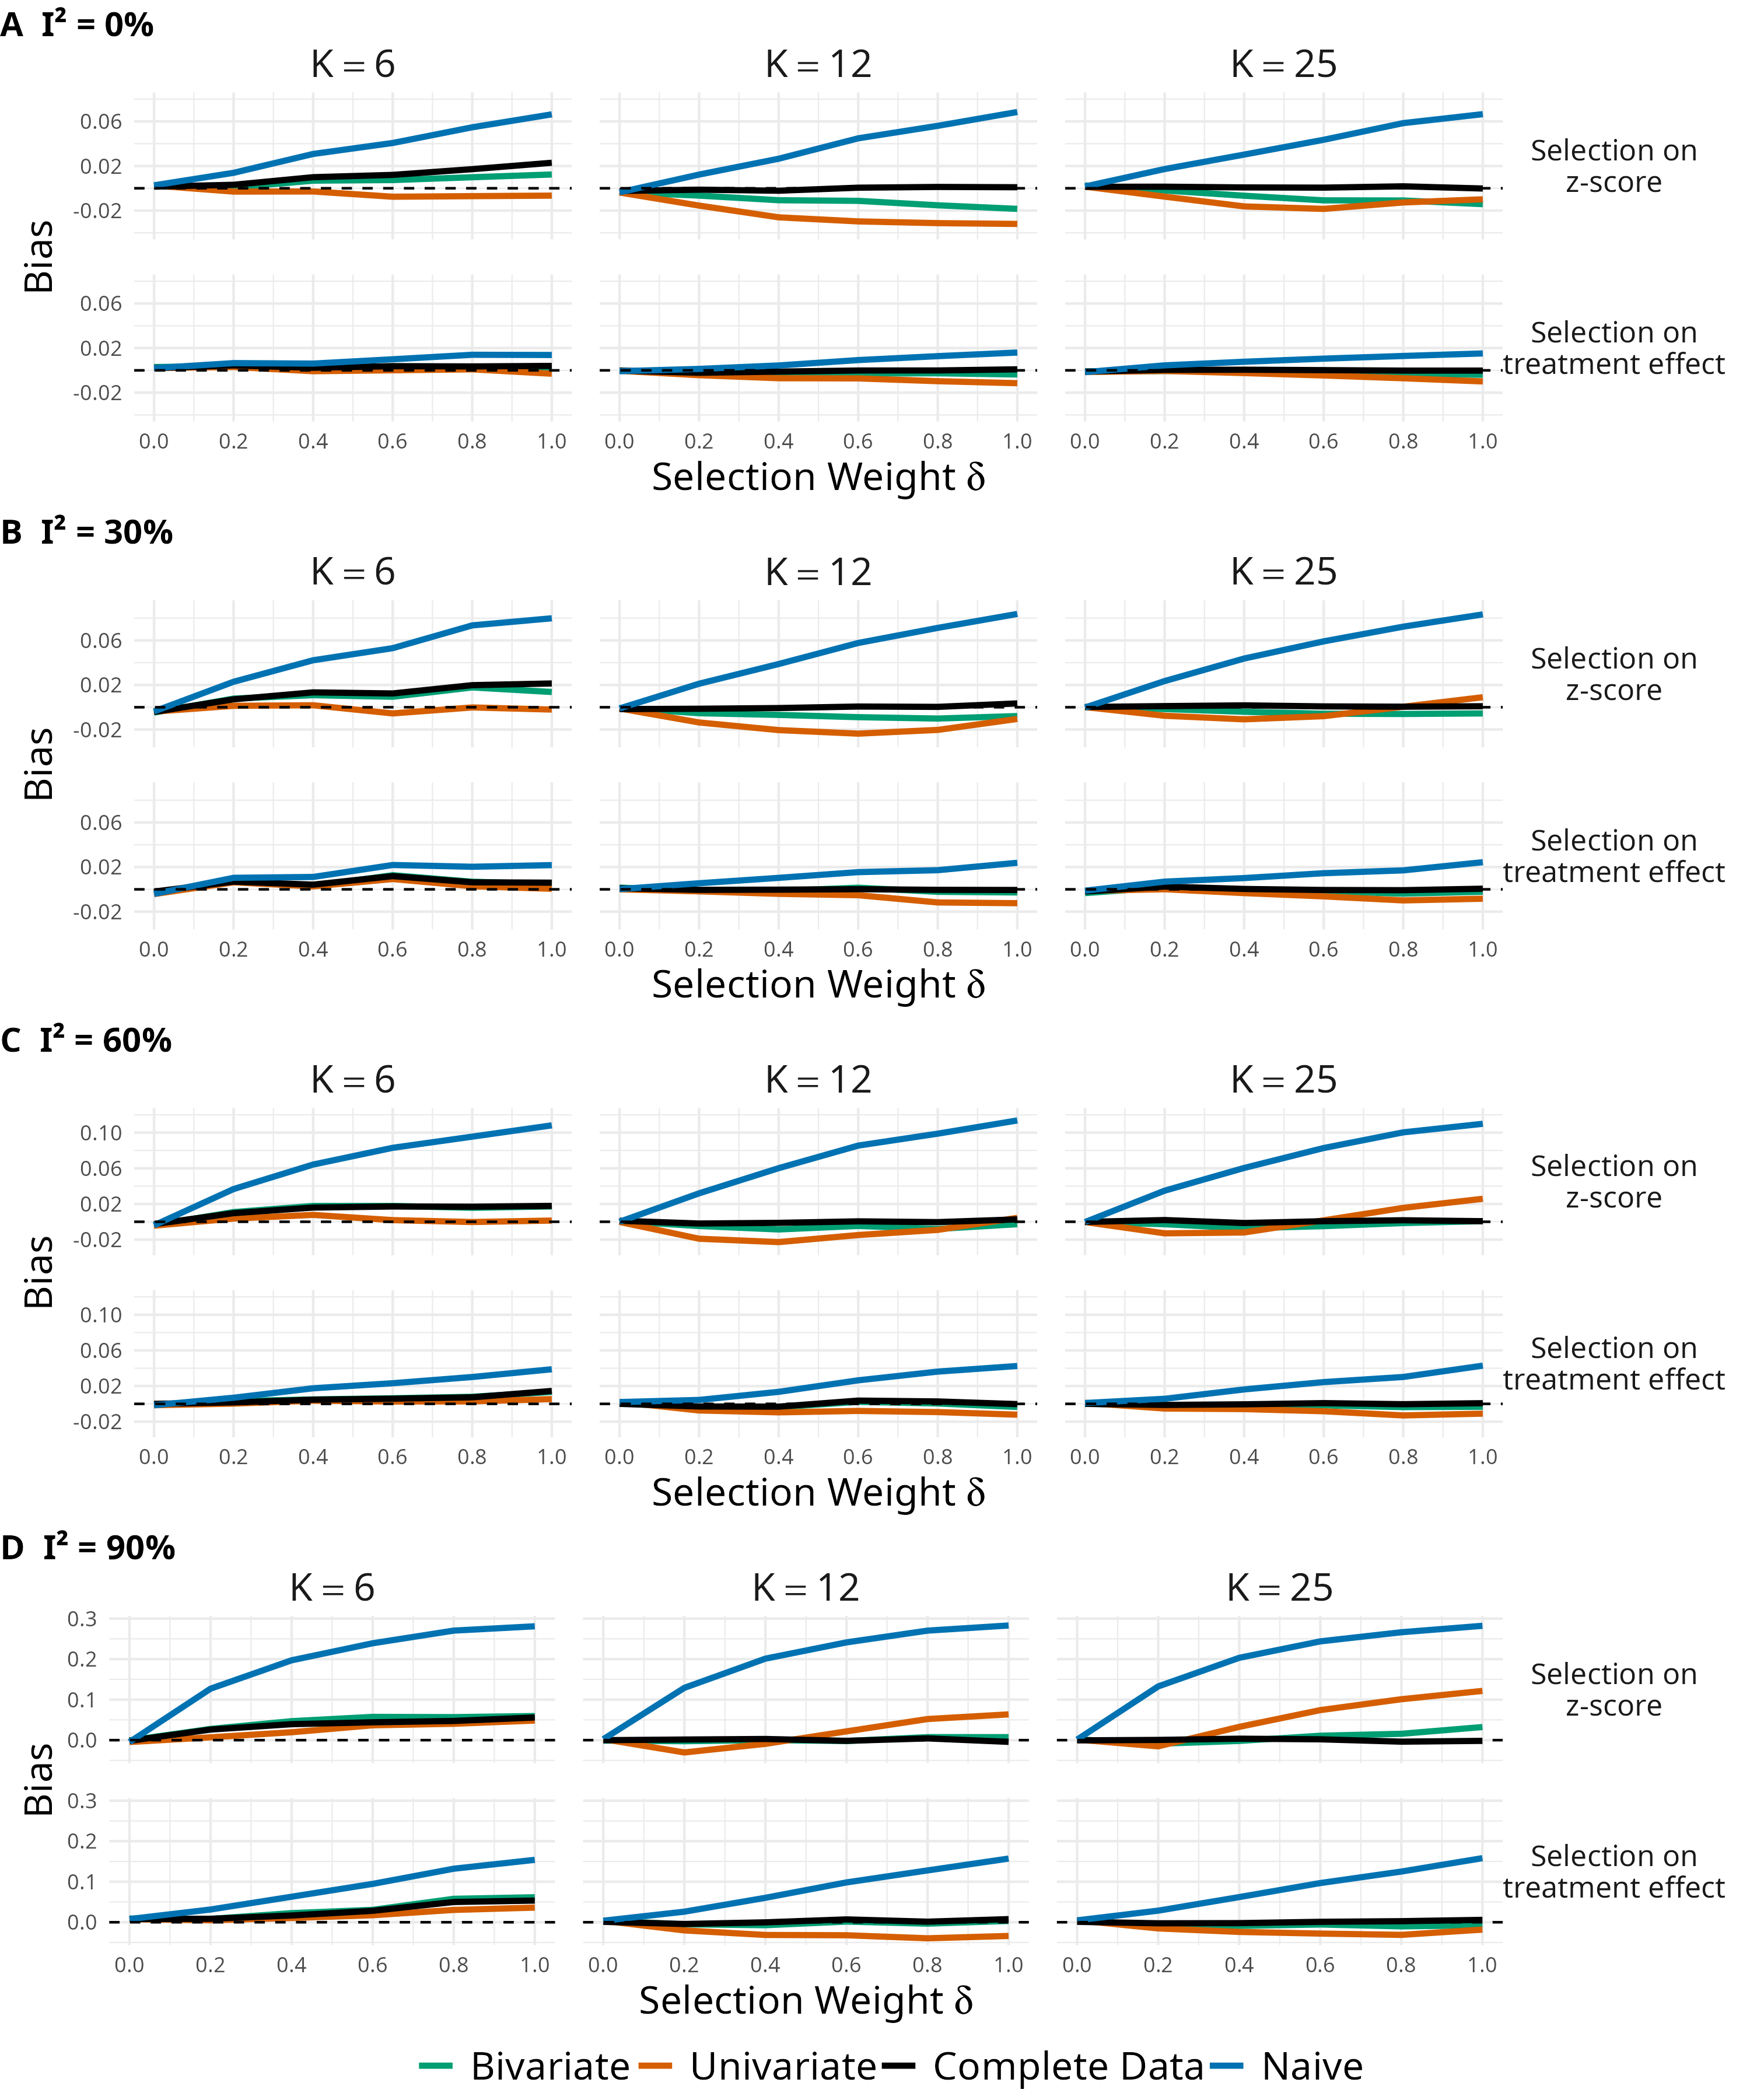
\includegraphics[width = 1\linewidth]{figures/Supp_SimStudy_Bias_p04.png}
\end{figure}

\begin{figure}[!ht]
\centering
\caption{Simulation results for MSE of four MA estimates of the treatment effect for outcome 1 under ORB for $\theta_1 = \theta_2 = 0.4$, $\rho_B = \rho_W = 0.8$ and $p_1 = 40\%$. Results are shown for varying numbers of studies, heterogeneity levels, selection type, and an increasing selection parameter.}
\label{fig:App_MSE_p04}
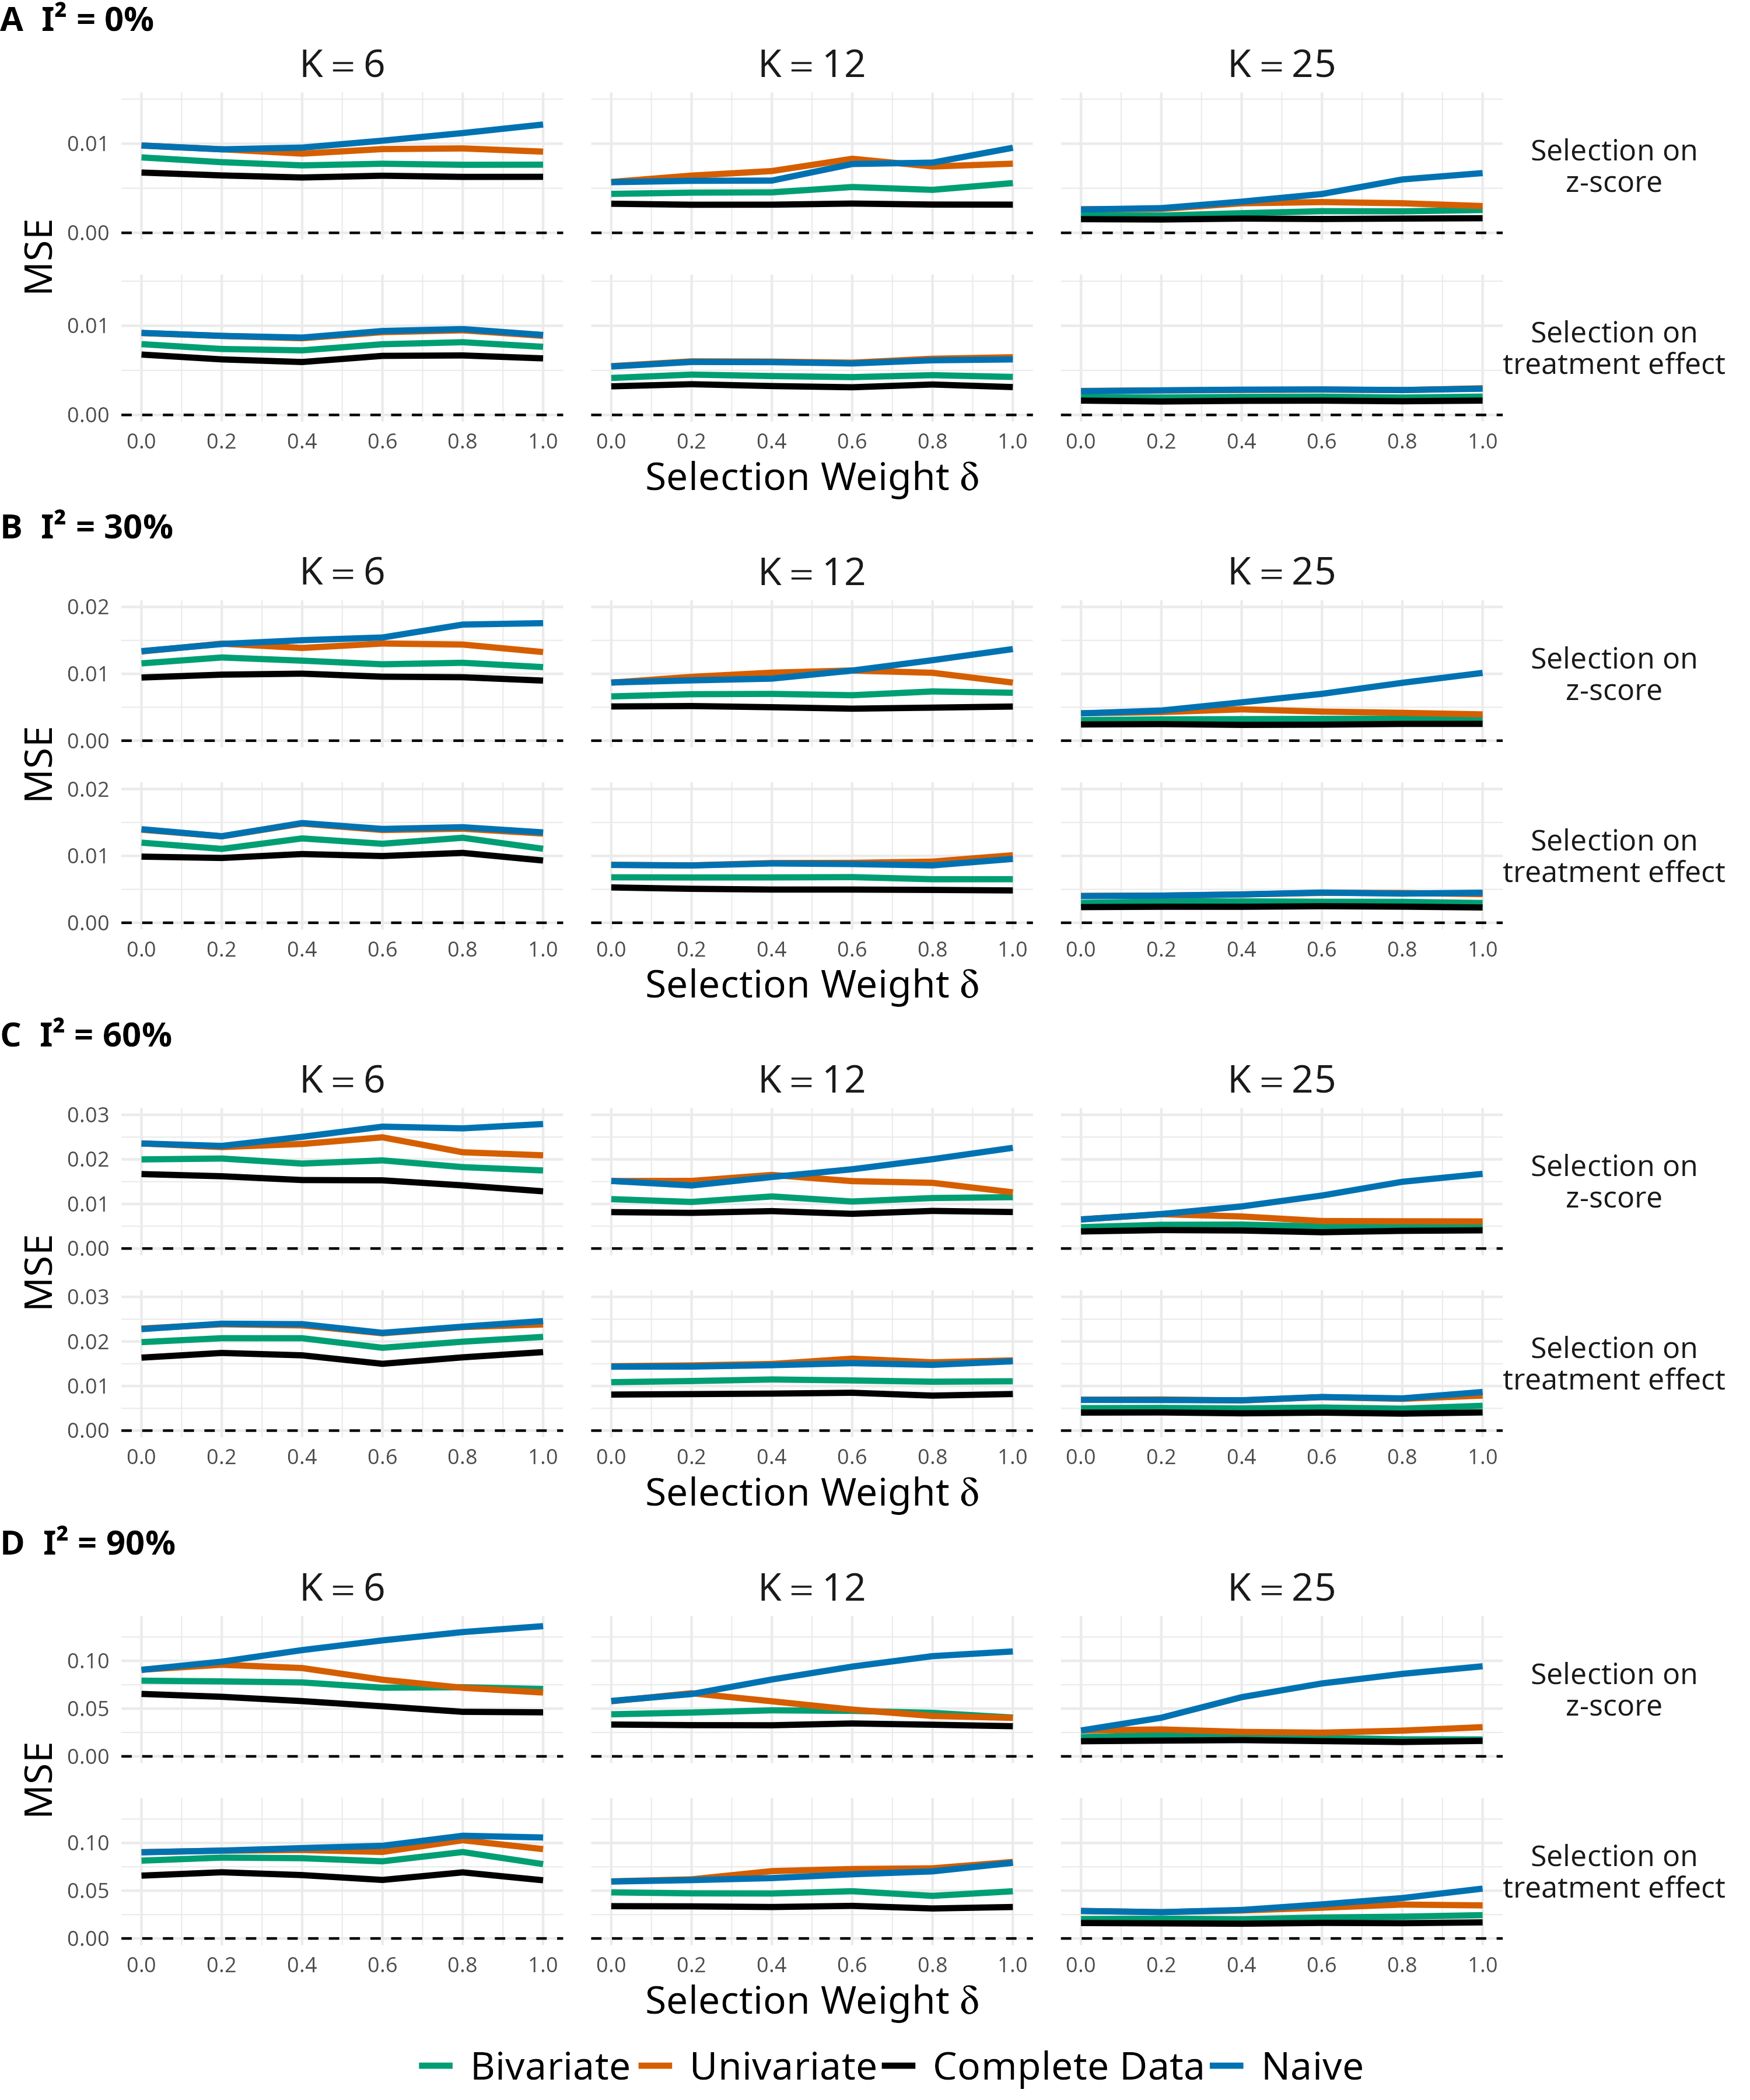
\includegraphics[width = 1\linewidth]{figures/Supp_SimStudy_MSE_p04.png}
\end{figure}

\begin{figure}[!ht]
\centering
\caption{Simulation results for CI width of four MA estimates of the treatment effect for outcome 1 under ORB for $\theta_1 = \theta_2 = 0.4$, $\rho_B = \rho_W = 0.8$ and $p_1 = 40\%$. Results are shown for varying numbers of studies, heterogeneity levels, selection type, and an increasing selection parameter.}
\label{fig:App_CIWidth_p04}
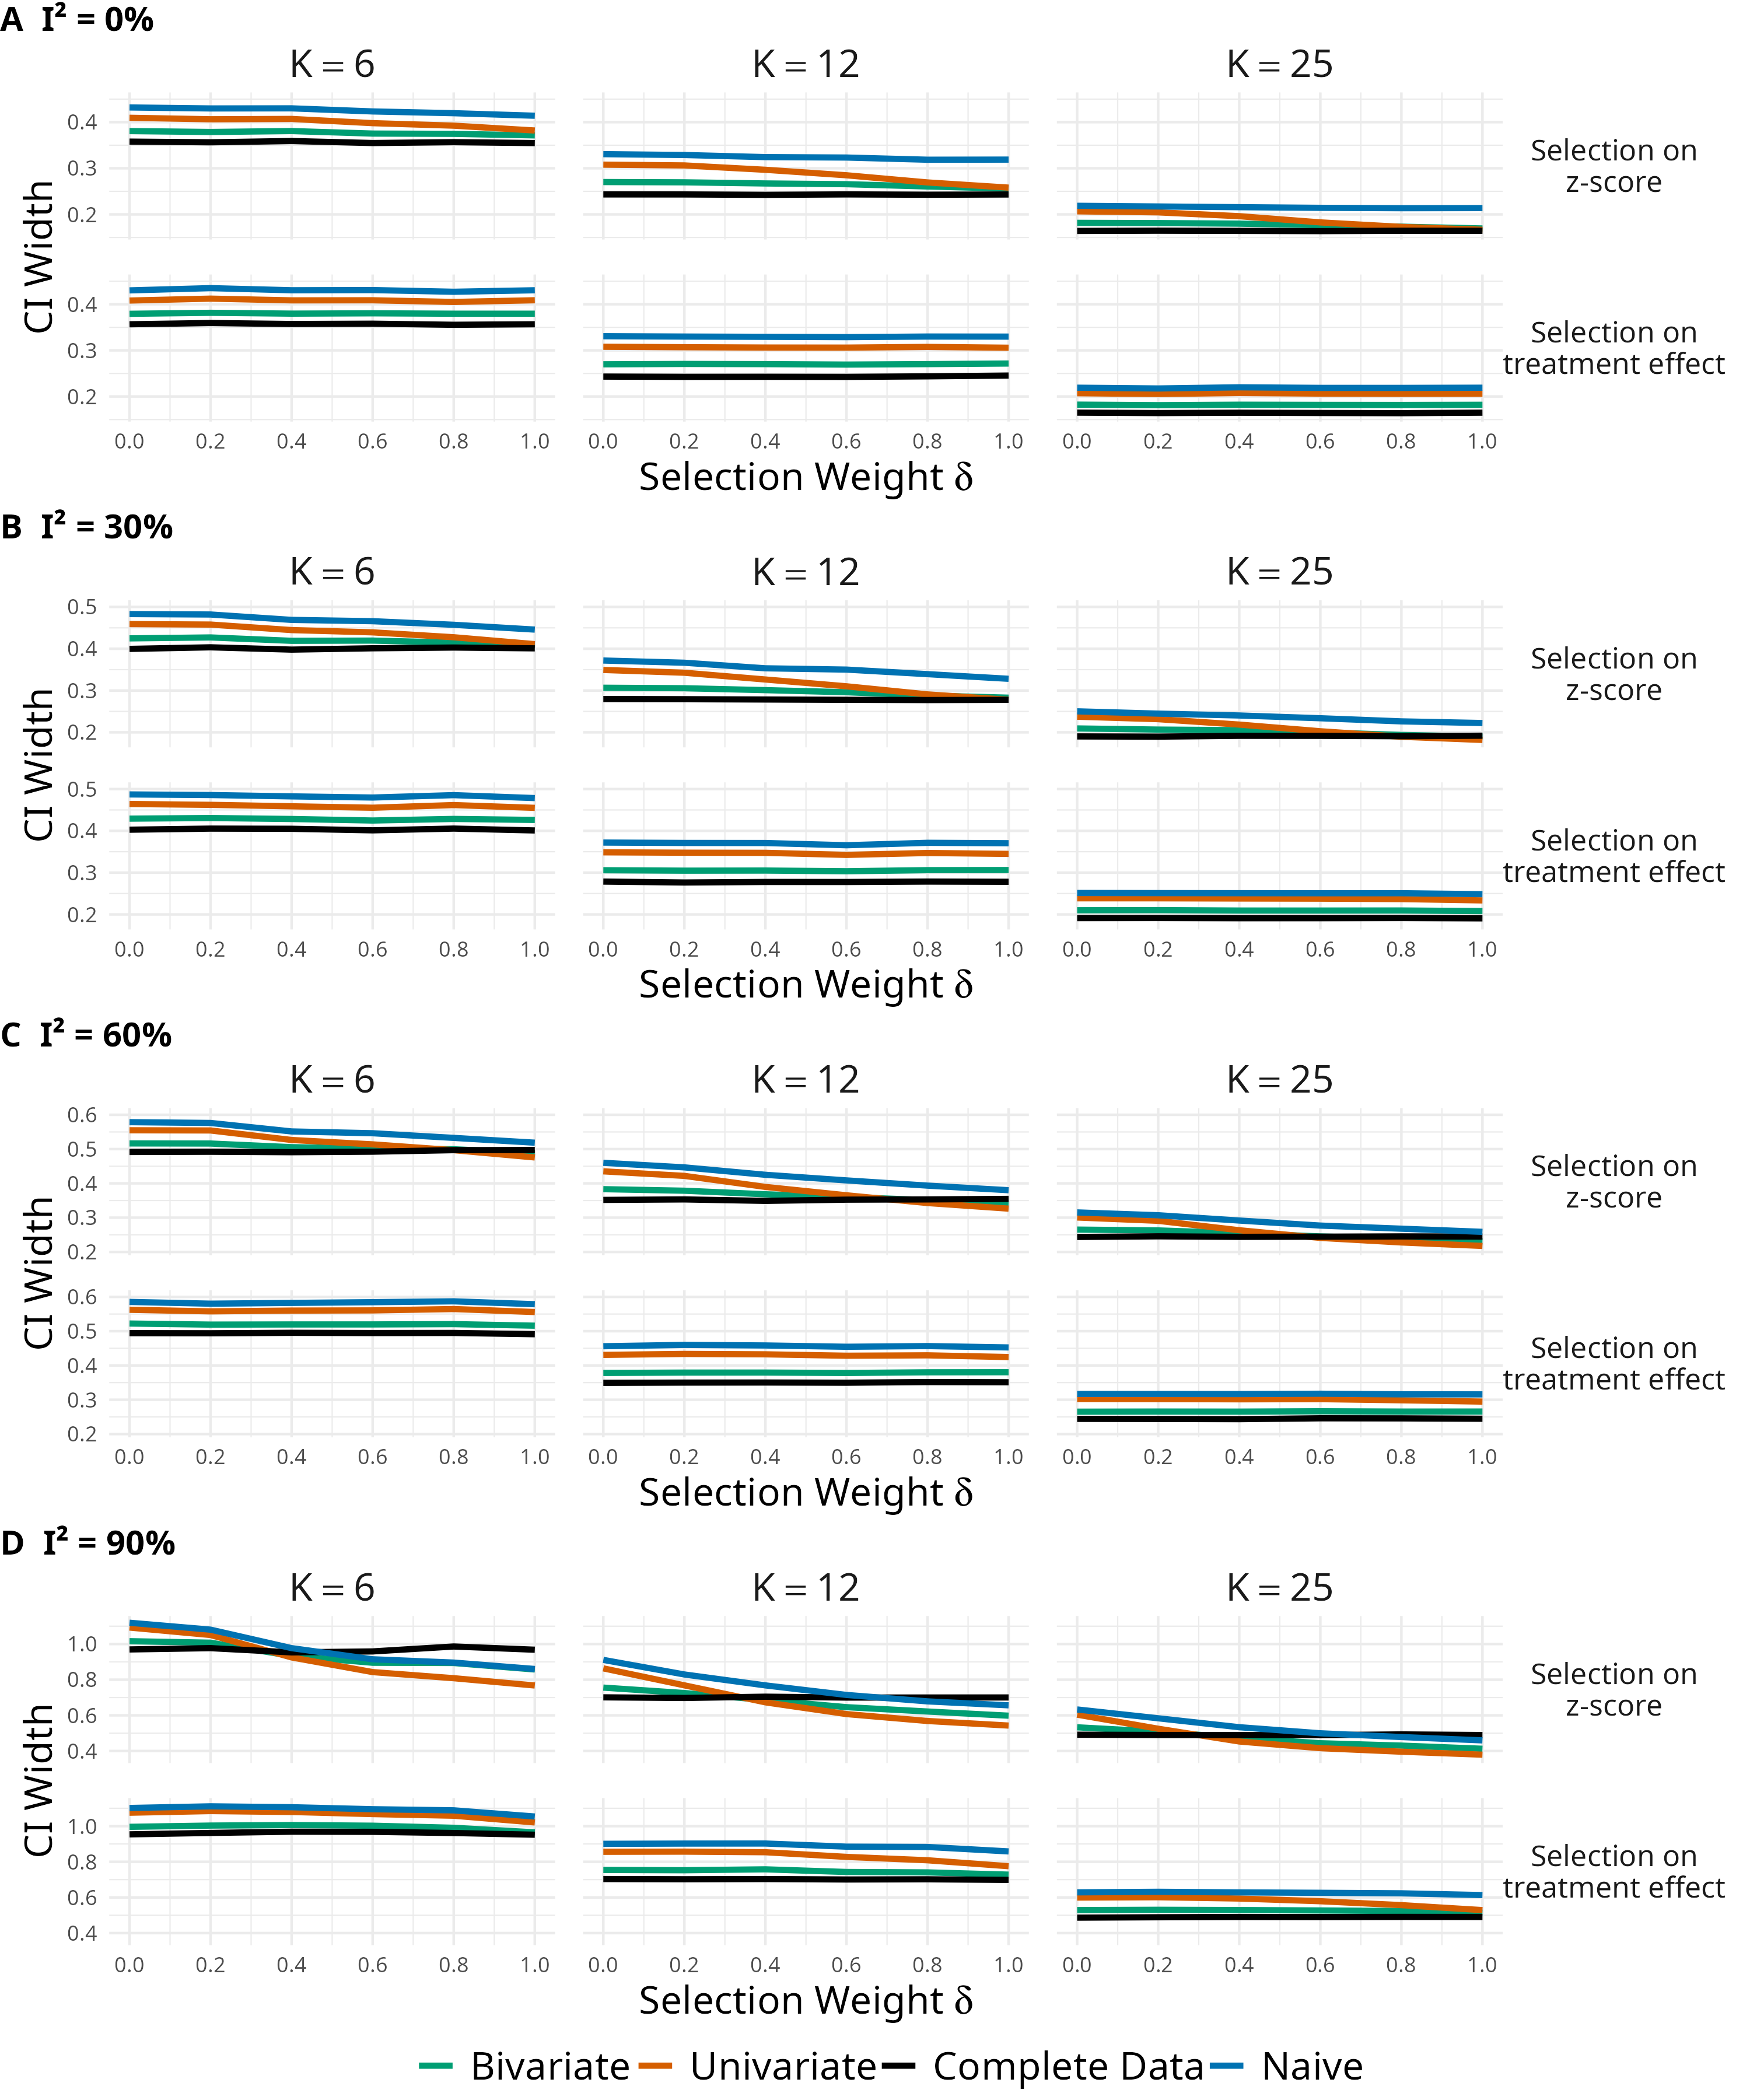
\includegraphics[width = 1\linewidth]{figures/Supp_SimStudy_CIWidth_p04.png}
\end{figure}

\begin{figure}[!ht]
\centering
\caption{Simulation results for coverage of four MA estimates of the treatment effect for outcome 1 under ORB for $\theta_1 = \theta_2 = 0.4$, $\rho_B = \rho_W = 0.8$ and $p_1 = 40\%$. Results are shown for varying numbers of studies, heterogeneity levels, selection type, and an increasing selection parameter.}
\label{fig:App_Coverage_p04}
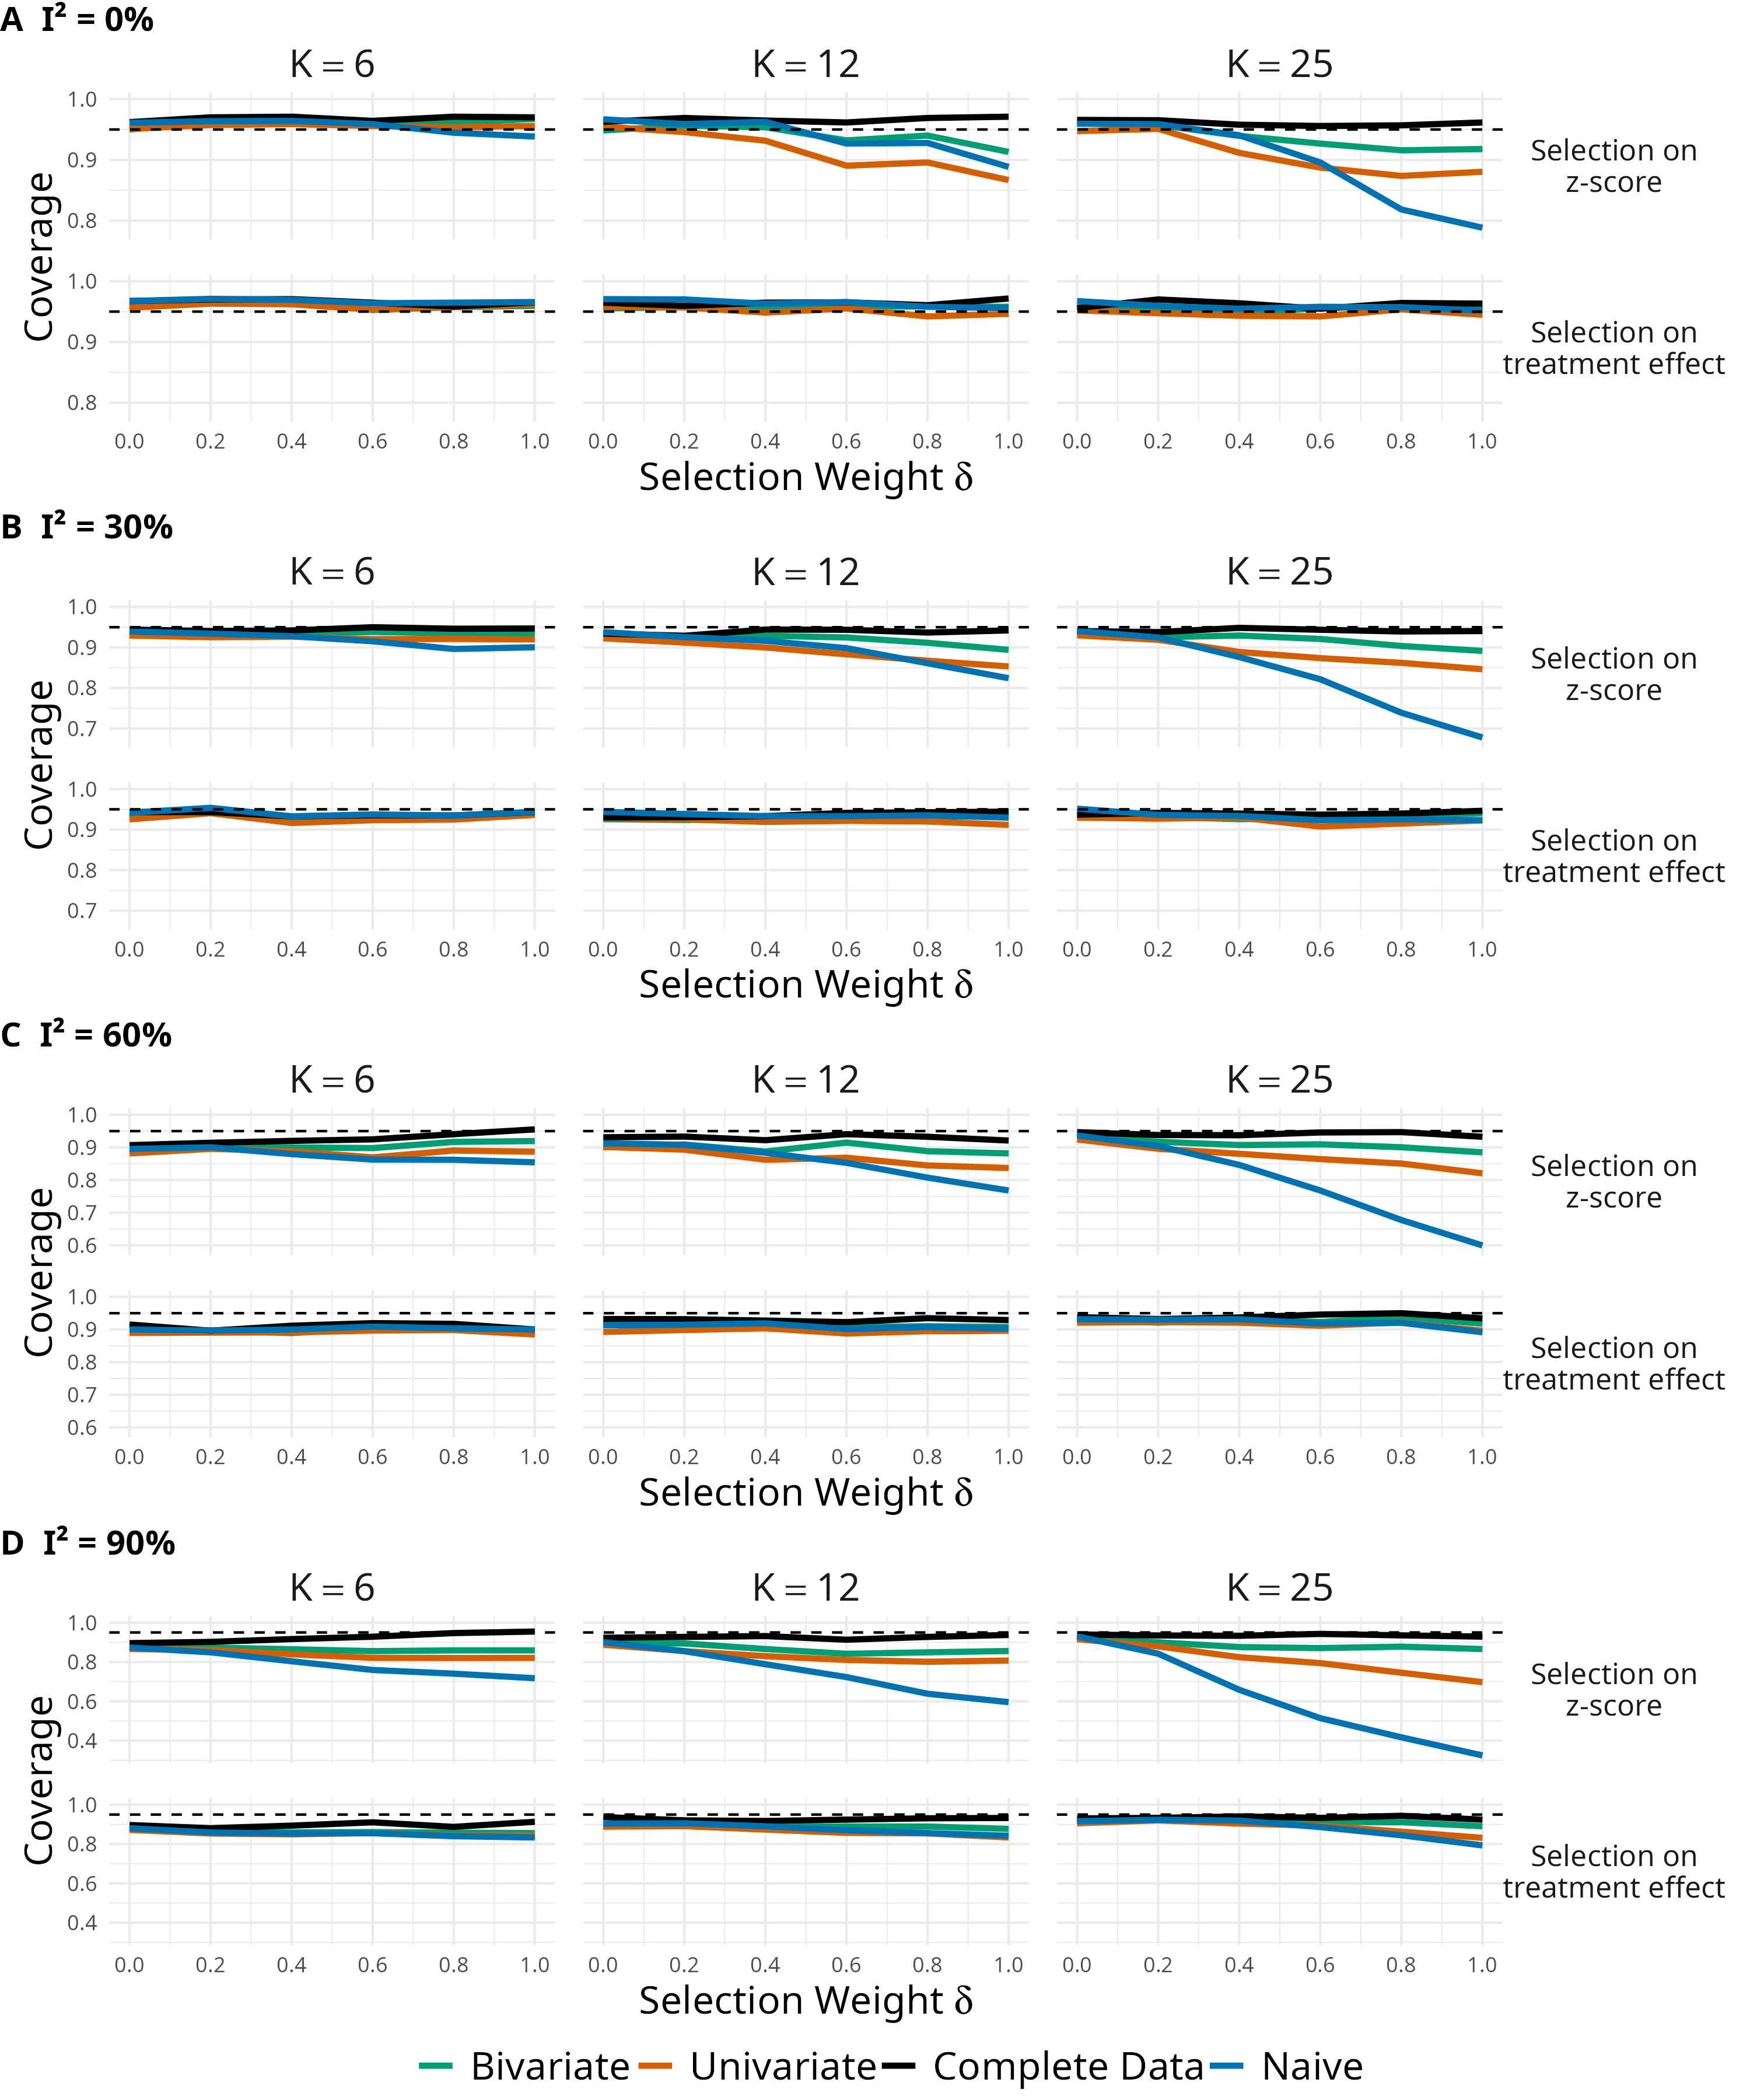
\includegraphics[width = 1\linewidth]{figures/Supp_SimStudy_Coverage_p04.png}
\end{figure}

\clearpage

\subsection{\mycolor{Heterogeneous sample sizes for main scenario}}
\label{heterogeneous}

\mycolor{To assess the robustness of the simulation results to variation in sample size, we additionally considered a heterogeneous sample size scenario. In this scenario, one study $i^\ast$ within each simulated meta-analysis is assigned a total sample size of $n_{i^\ast}=500$, with $n_{ti^\ast}=n_{ci^\ast}=250$, while all remaining studies retain the original sample size of $n_i=100$, with $n_{ti}=n_{ci}=50.$ Thus, one study in each simulated meta-analysis has a total sample size that is five times larger than that of the other studies. The larger study is generated according to the same data-generating mechanism for the treatment effects and within-study correlation as the other studies. Its larger sample size results in greater statistical precision. Heterogeneous study sizes are considered only for the main simulation scenario, that is, for $\theta_1 = \theta_2 = 0.4$, $\rho_W = \rho_B = 0.8$, $K  \in \{6, 12, 25\}$ and $p_1 = 20\%$, with $I^2$ \{0\%, 30\%, 60\%, 90\%\}, the selection parameter $\delta_\text{sim} = \delta_\text{est} = \{0, 0.2, 0.4, 0.6, 0.8, 1\}$ and the selection on the treatment effect and $z$-score.}

\mycolor{The true study-specific effects $\boldsymbol{\theta}_i$ and the within-study correlation $\rho_W$ are generated as in the main scenario. Only the within-study covariance matrices depend on the sample size:
\begin{equation*}
    \boldsymbol{\Sigma}_i \sim \mathcal{W}_2(d_i, \boldsymbol{V}_i), \qquad
    d_i = n_i - 2, \qquad
    \boldsymbol{V}_i = \frac{1}{(n_i/2 - 1)\, n_i/2}
    \begin{pmatrix} 1 & \rho_W \\ \rho_W & 1 \end{pmatrix},
\end{equation*}
so that $\mathbb{E}(\boldsymbol{\Sigma}_i) = d_i \boldsymbol{V}_i$ has marginal variances $4/n_i$. This gives $d_i = 98$ and $\sigma^2_{ij} = 4/100 = 0.04$ for the standard studies, and $d_{i^\ast} = 498$ and $\sigma^2_{i^\ast j} = 4/500 = 0.008$ for the large study.}

\mycolor{Selective reporting follows the same model as in the main scenario. Because the expected selection variable now differs between studies, the intercept $\alpha_1$ is calibrated using the average expected selection variable across the $K$ studies, $\alpha_1 = \operatorname{logit}(1 - p_1) - \delta_{1,\mathrm{sim}} \overline{\mathbb{E}(s_1)}$, $\overline{\mathbb{E}(s_1)} = \frac{1}{K} \sum_{i=1}^{K} \mathbb{E}(s_{i1})$}.
\mycolor{Sample size heterogeneity does not alter the calibration for selection on the treatment effect, since $\mathbb{E}(\hat{\theta}_{i1}) = \theta_1$ for all studies irrespective of sample size, $\overline{\mathbb{E}(s_1)} = \theta_1$. However, the expected standardized effect depends on the study sample size $n_i$. With one large study ($n_{i^\ast}=500$) and $K-1$ standard studies ($n_i=100$), the average expected $z$-score is
    \begin{equation*}
        \overline{\mathbb{E}(z_1)} = \frac{1}{K} \left[ \frac{\theta_1}{\sqrt{4/500 + \tau_1^2}} + (K - 1)\, \frac{\theta_1}{\sqrt{4/100 + \tau_1^2}} \right].
    \end{equation*}}

\begin{figure}[!ht]
\centering
\caption{Simulation results for bias of four MA estimates of the treatment effect for outcome 1 under ORB for heterogeneous sample sizes for $\theta_1 = \theta_2 = 0.4$, $\rho_B = \rho_W = 0.8$ and $p_1 = 20\%$. Results are shown for varying numbers of studies, heterogeneity levels, selection type, and an increasing selection parameter.}
\label{fig:App_Bias_het}
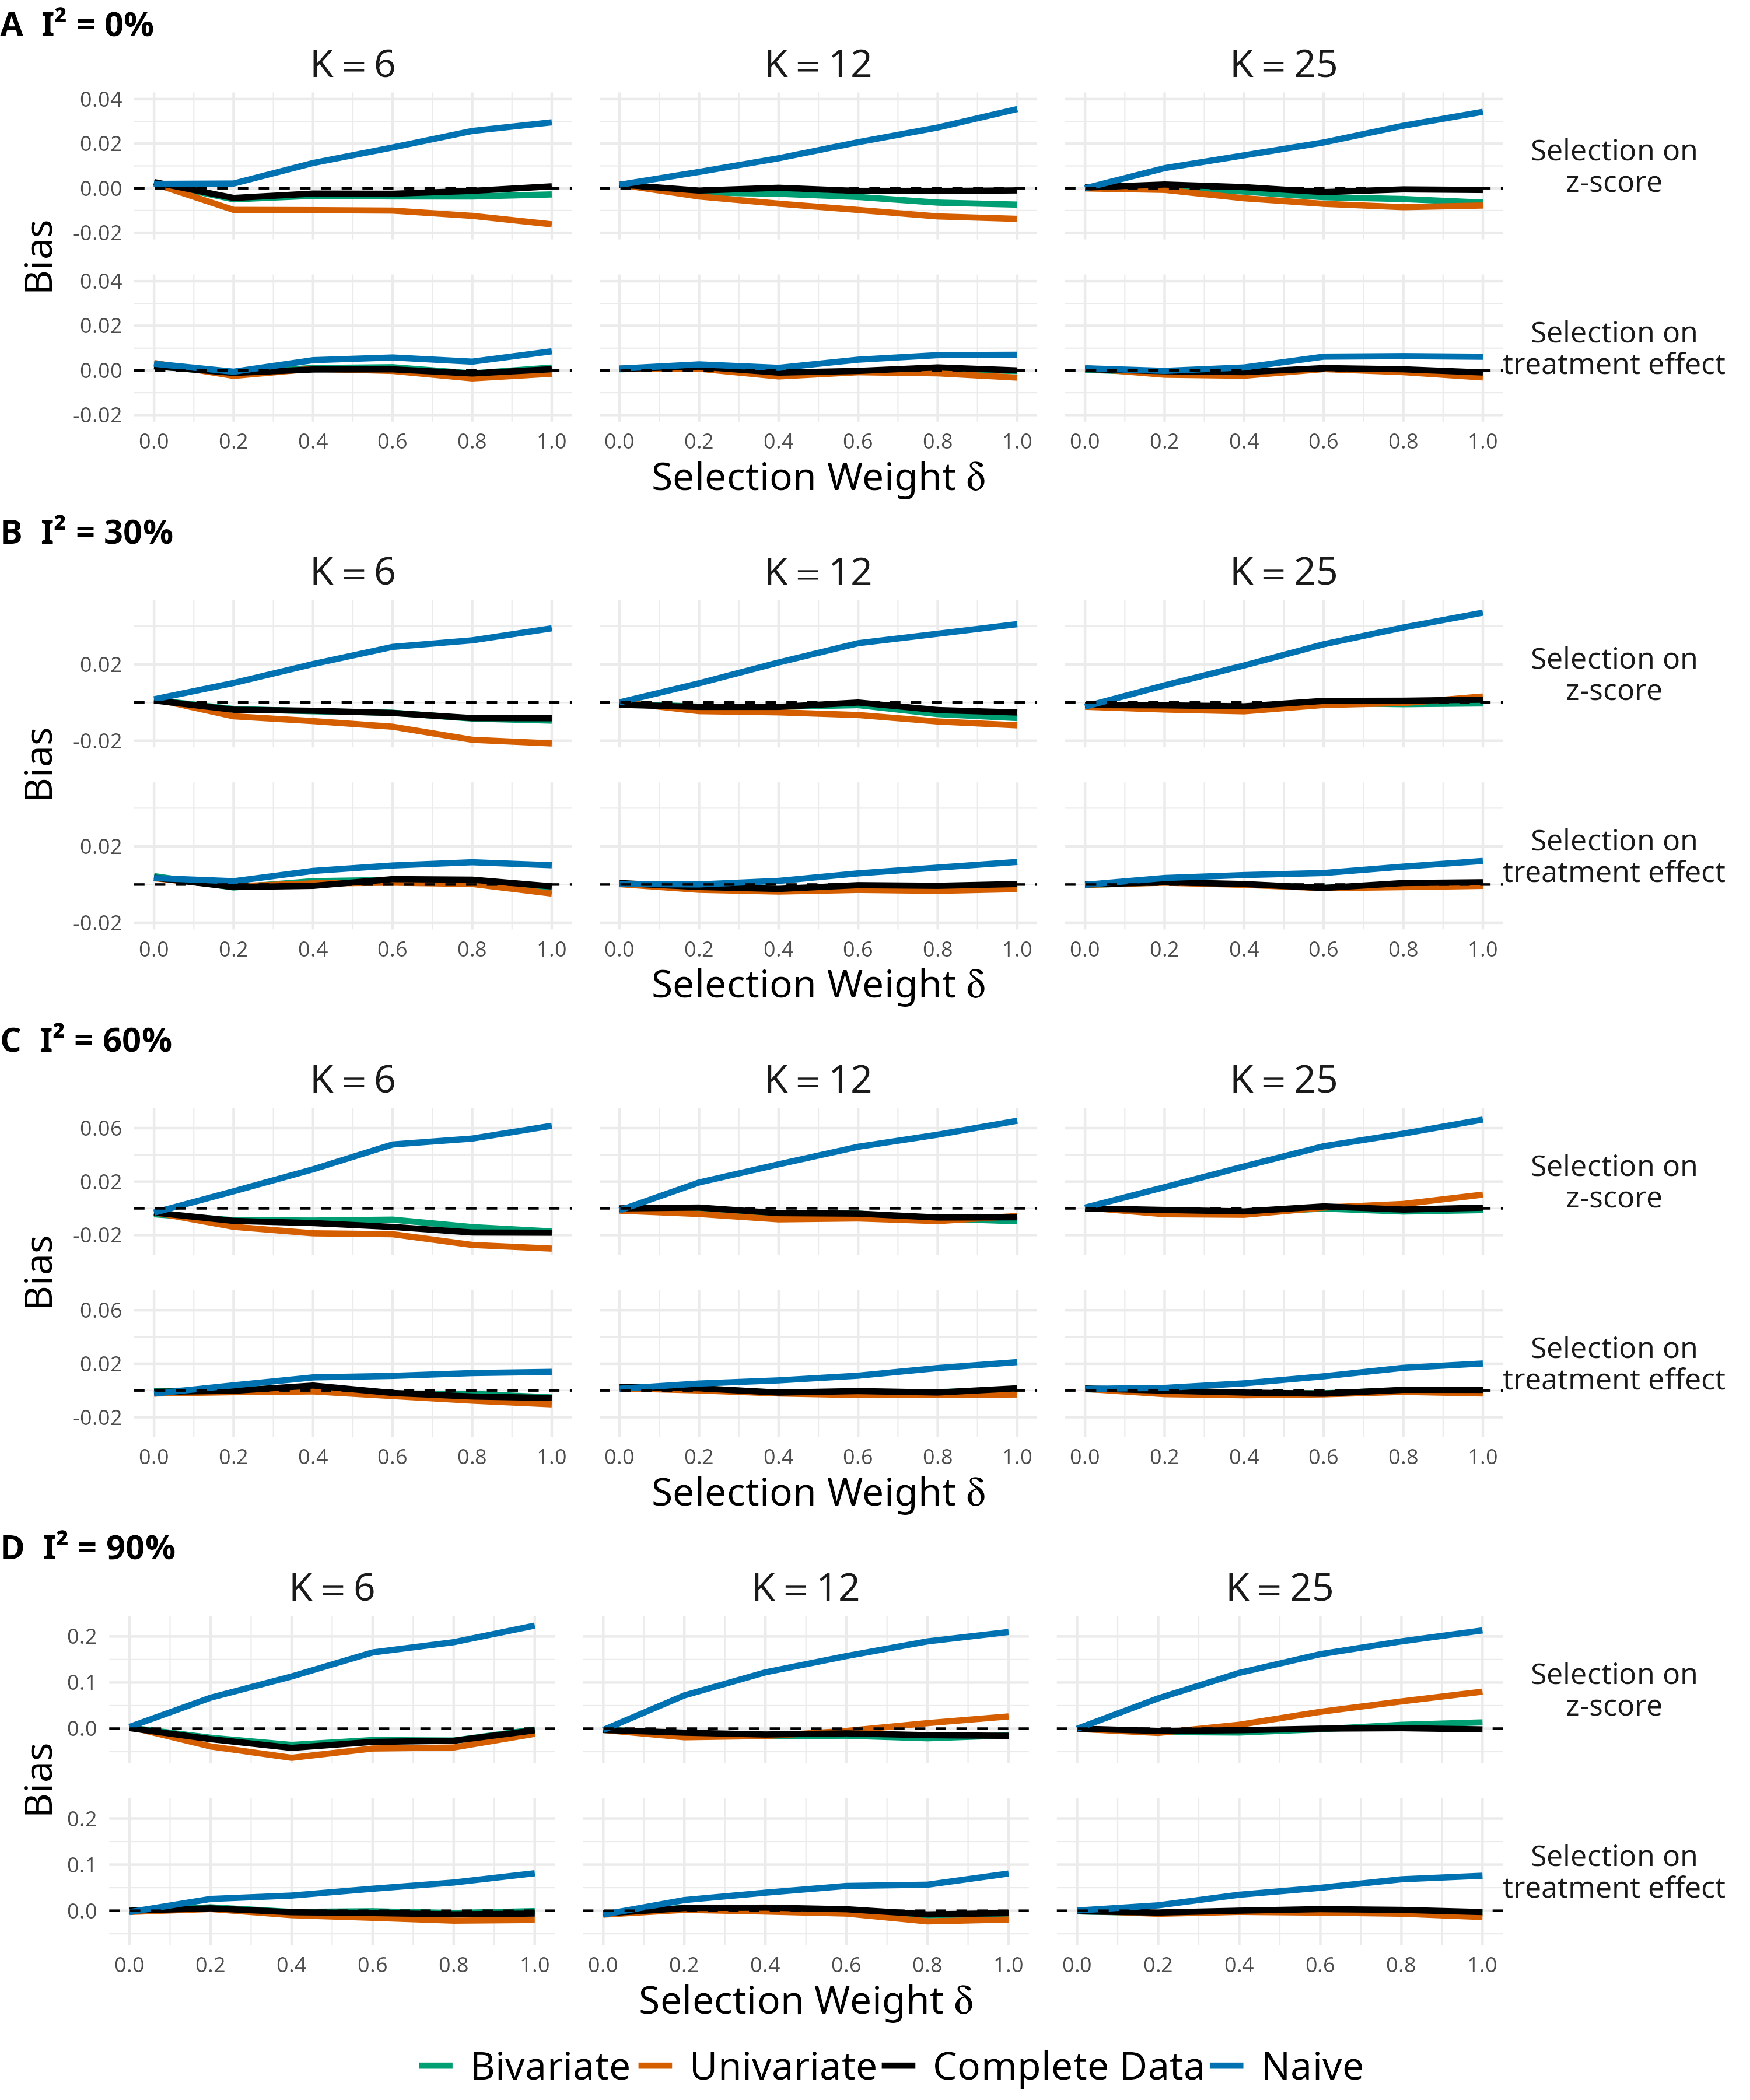
\includegraphics[width = 1\linewidth]{figures/Supp_SimStudy_Bias_het.png}
\end{figure}

\begin{figure}[!ht]
\centering
\caption{Simulation results for MSE of four MA estimates of the treatment effect for outcome 1 under ORB for heterogeneous sample sizes for $\theta_1 = \theta_2 = 0.4$, $\rho_B = \rho_W = 0.8$ and $p_1 = 20\%$. Results are shown for varying numbers of studies, heterogeneity levels, selection type, and an increasing selection parameter.}
\label{fig:App_MSE_het}
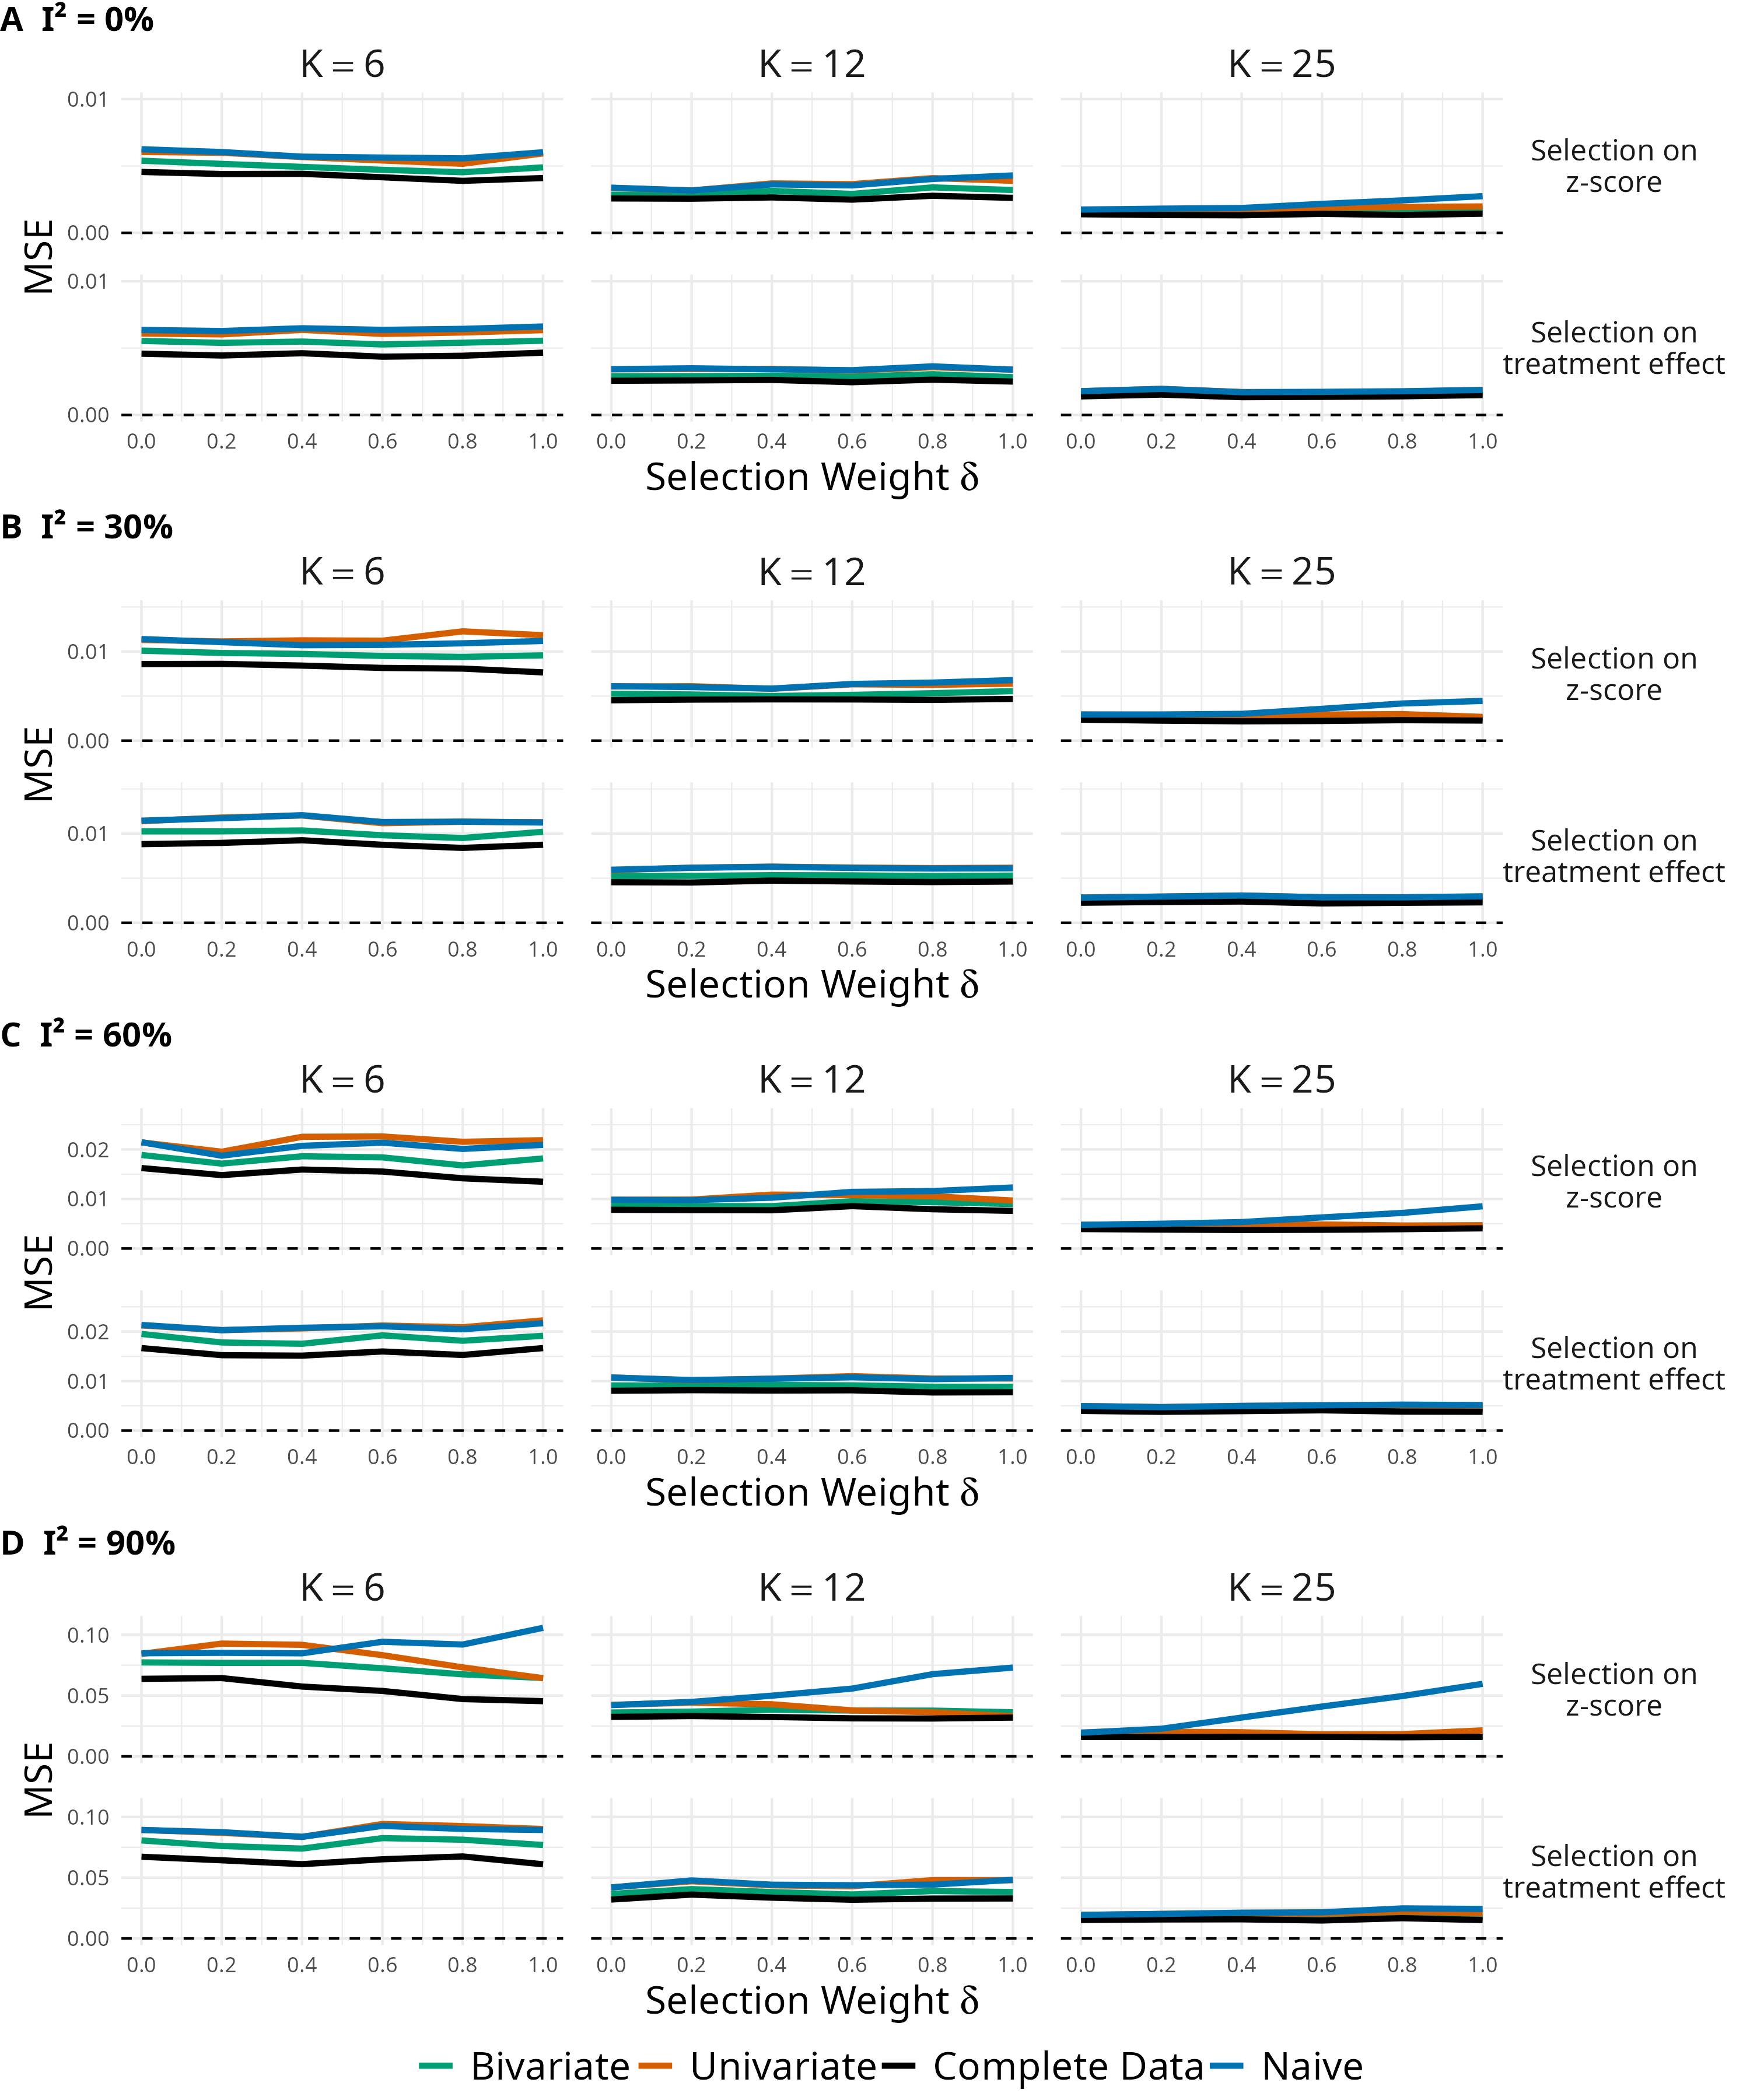
\includegraphics[width = 1\linewidth]{figures/Supp_SimStudy_MSE_het.png}
\end{figure}

\begin{figure}[!ht]
\centering
\caption{Simulation results for CI width of four MA estimates of the treatment effect for outcome 1 under ORB for heterogeneous sample sizes for $\theta_1 = \theta_2 = 0.4$, $\rho_B = \rho_W = 0.8$ and $p_1 = 20\%$. Results are shown for varying numbers of studies, heterogeneity levels, selection type, and an increasing selection parameter.}
\label{fig:App_CIWidth_het}
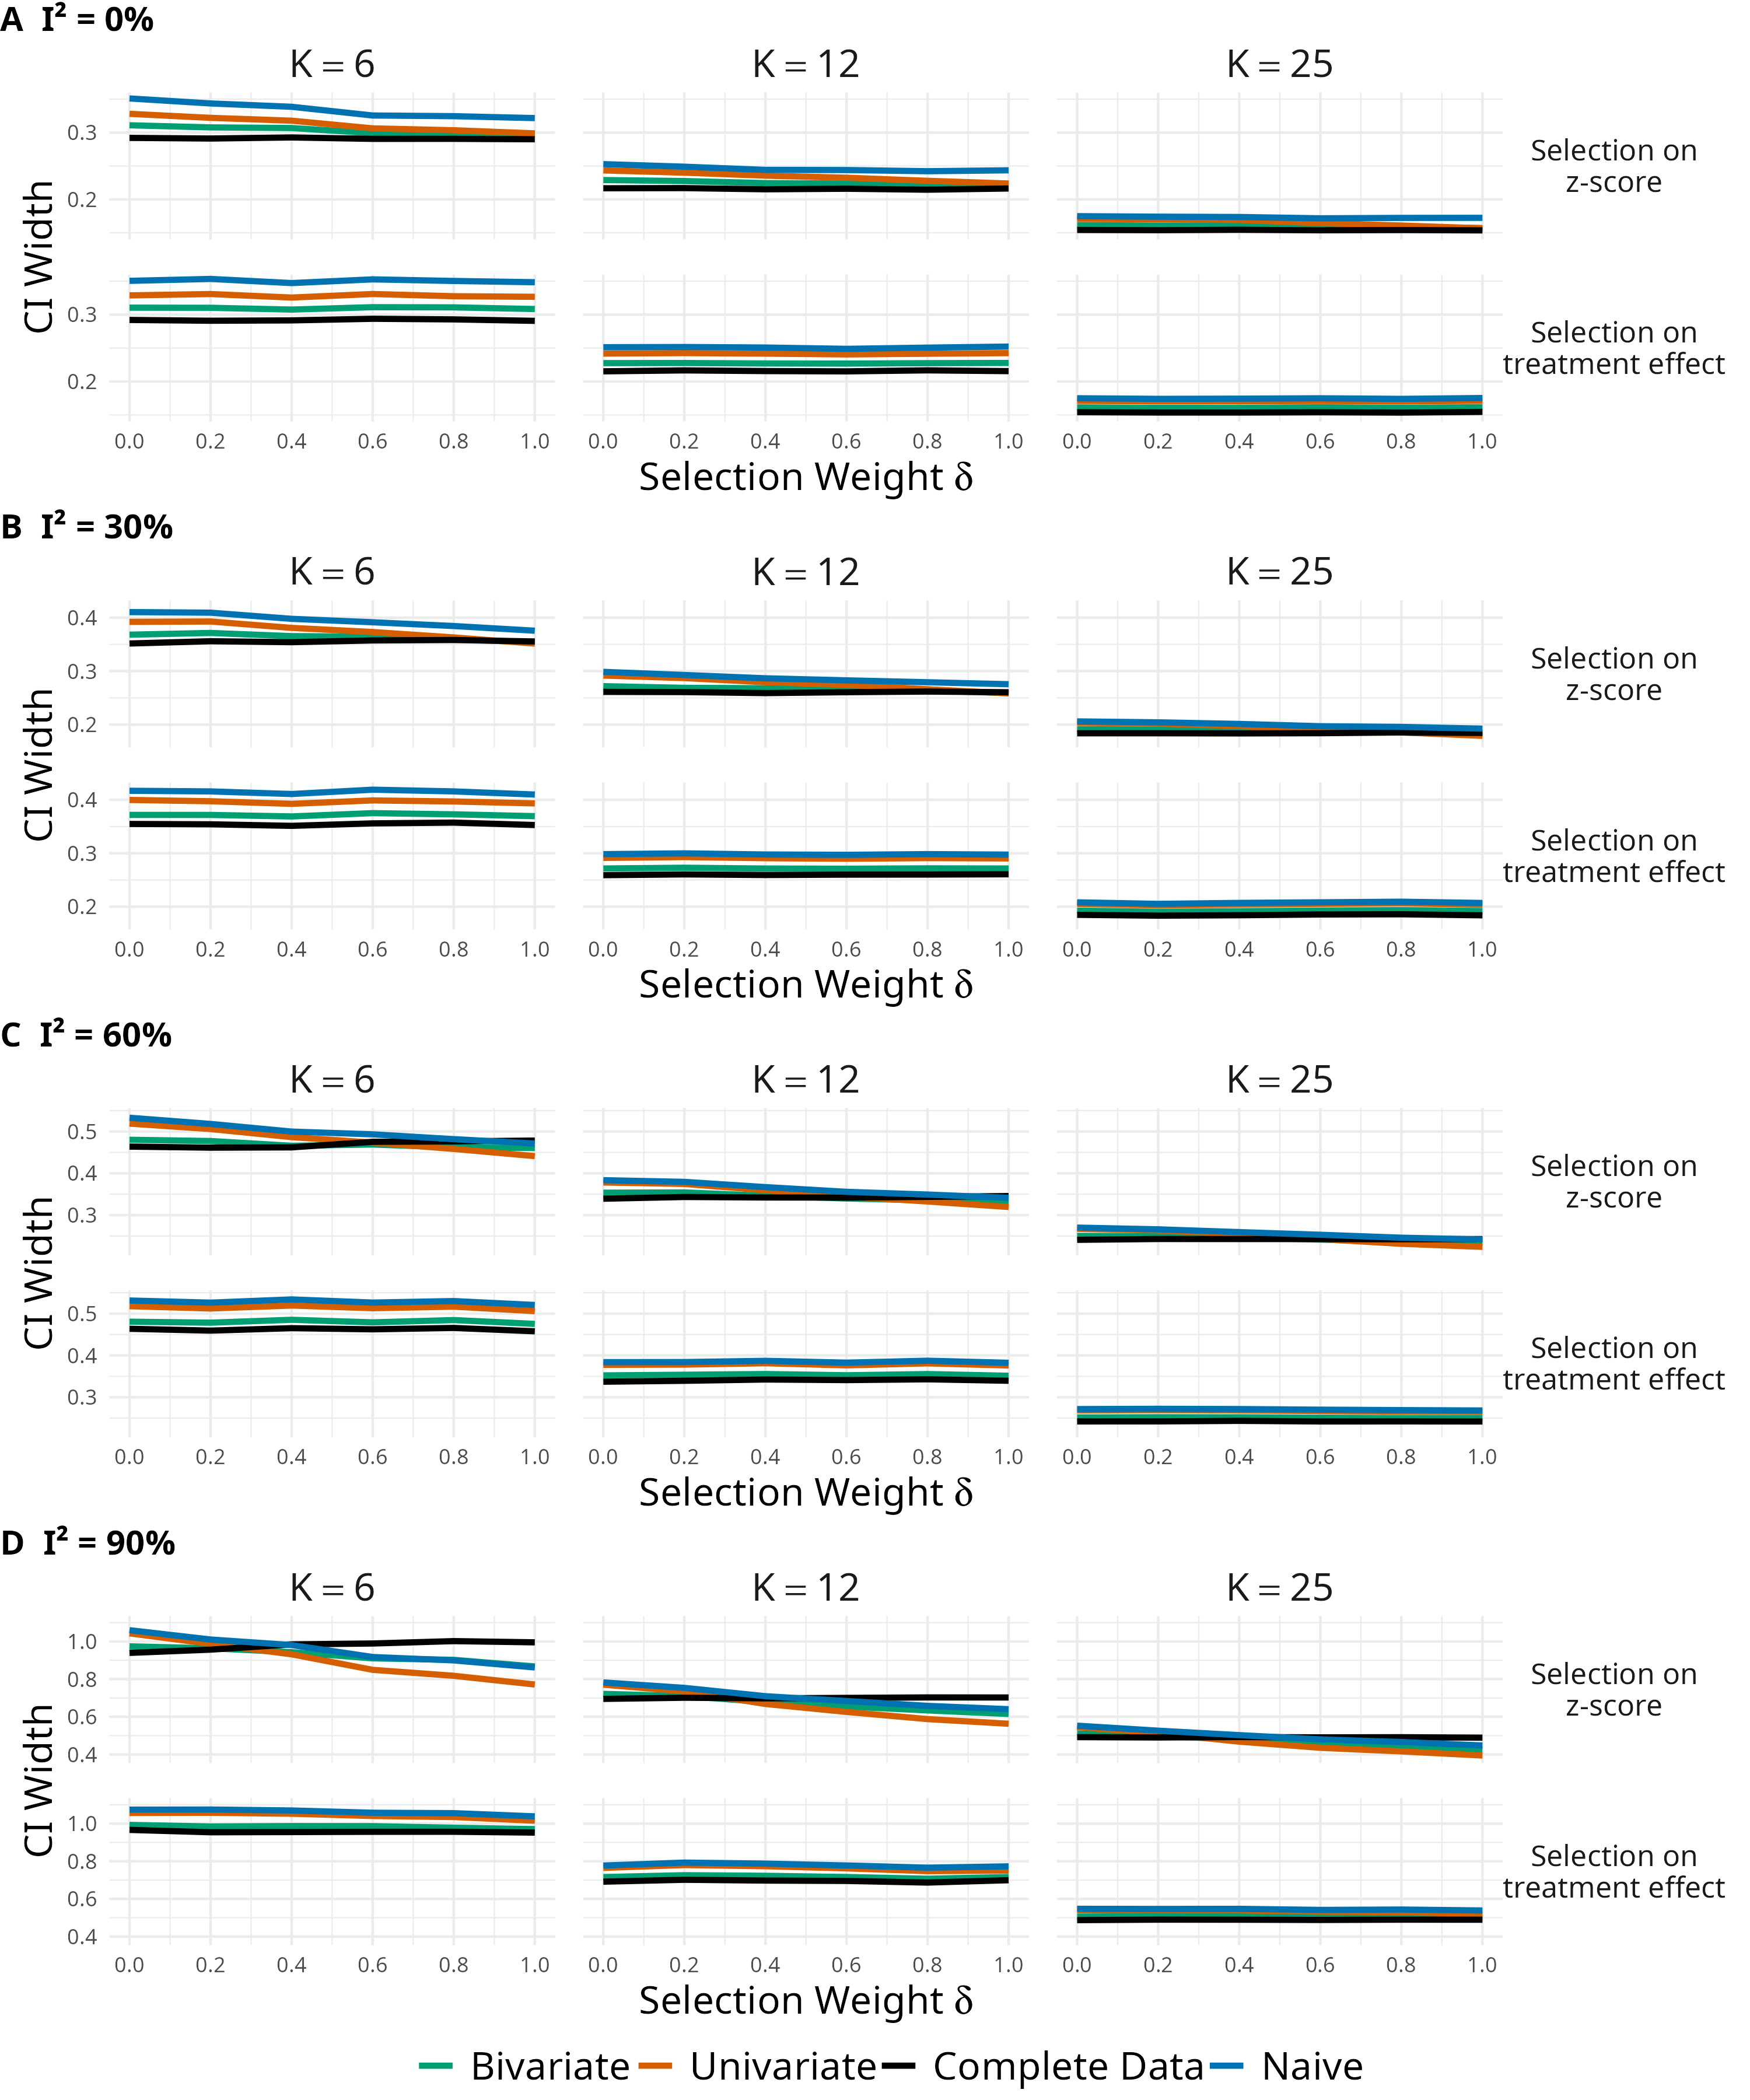
\includegraphics[width = 1\linewidth]{figures/Supp_SimStudy_CIWidth_het.png}
\end{figure}

\begin{figure}[!ht]
\centering
\caption{Simulation results for coverage of four MA estimates of the treatment effect for outcome 1 under ORB for heterogeneous sample sizes for $\theta_1 = \theta_2 = 0.4$, $\rho_B = \rho_W = 0.8$ and $p_1 = 20\%$. Results are shown for varying numbers of studies, heterogeneity levels, selection type, and an increasing selection parameter.}
\label{fig:App_Coverage_het}
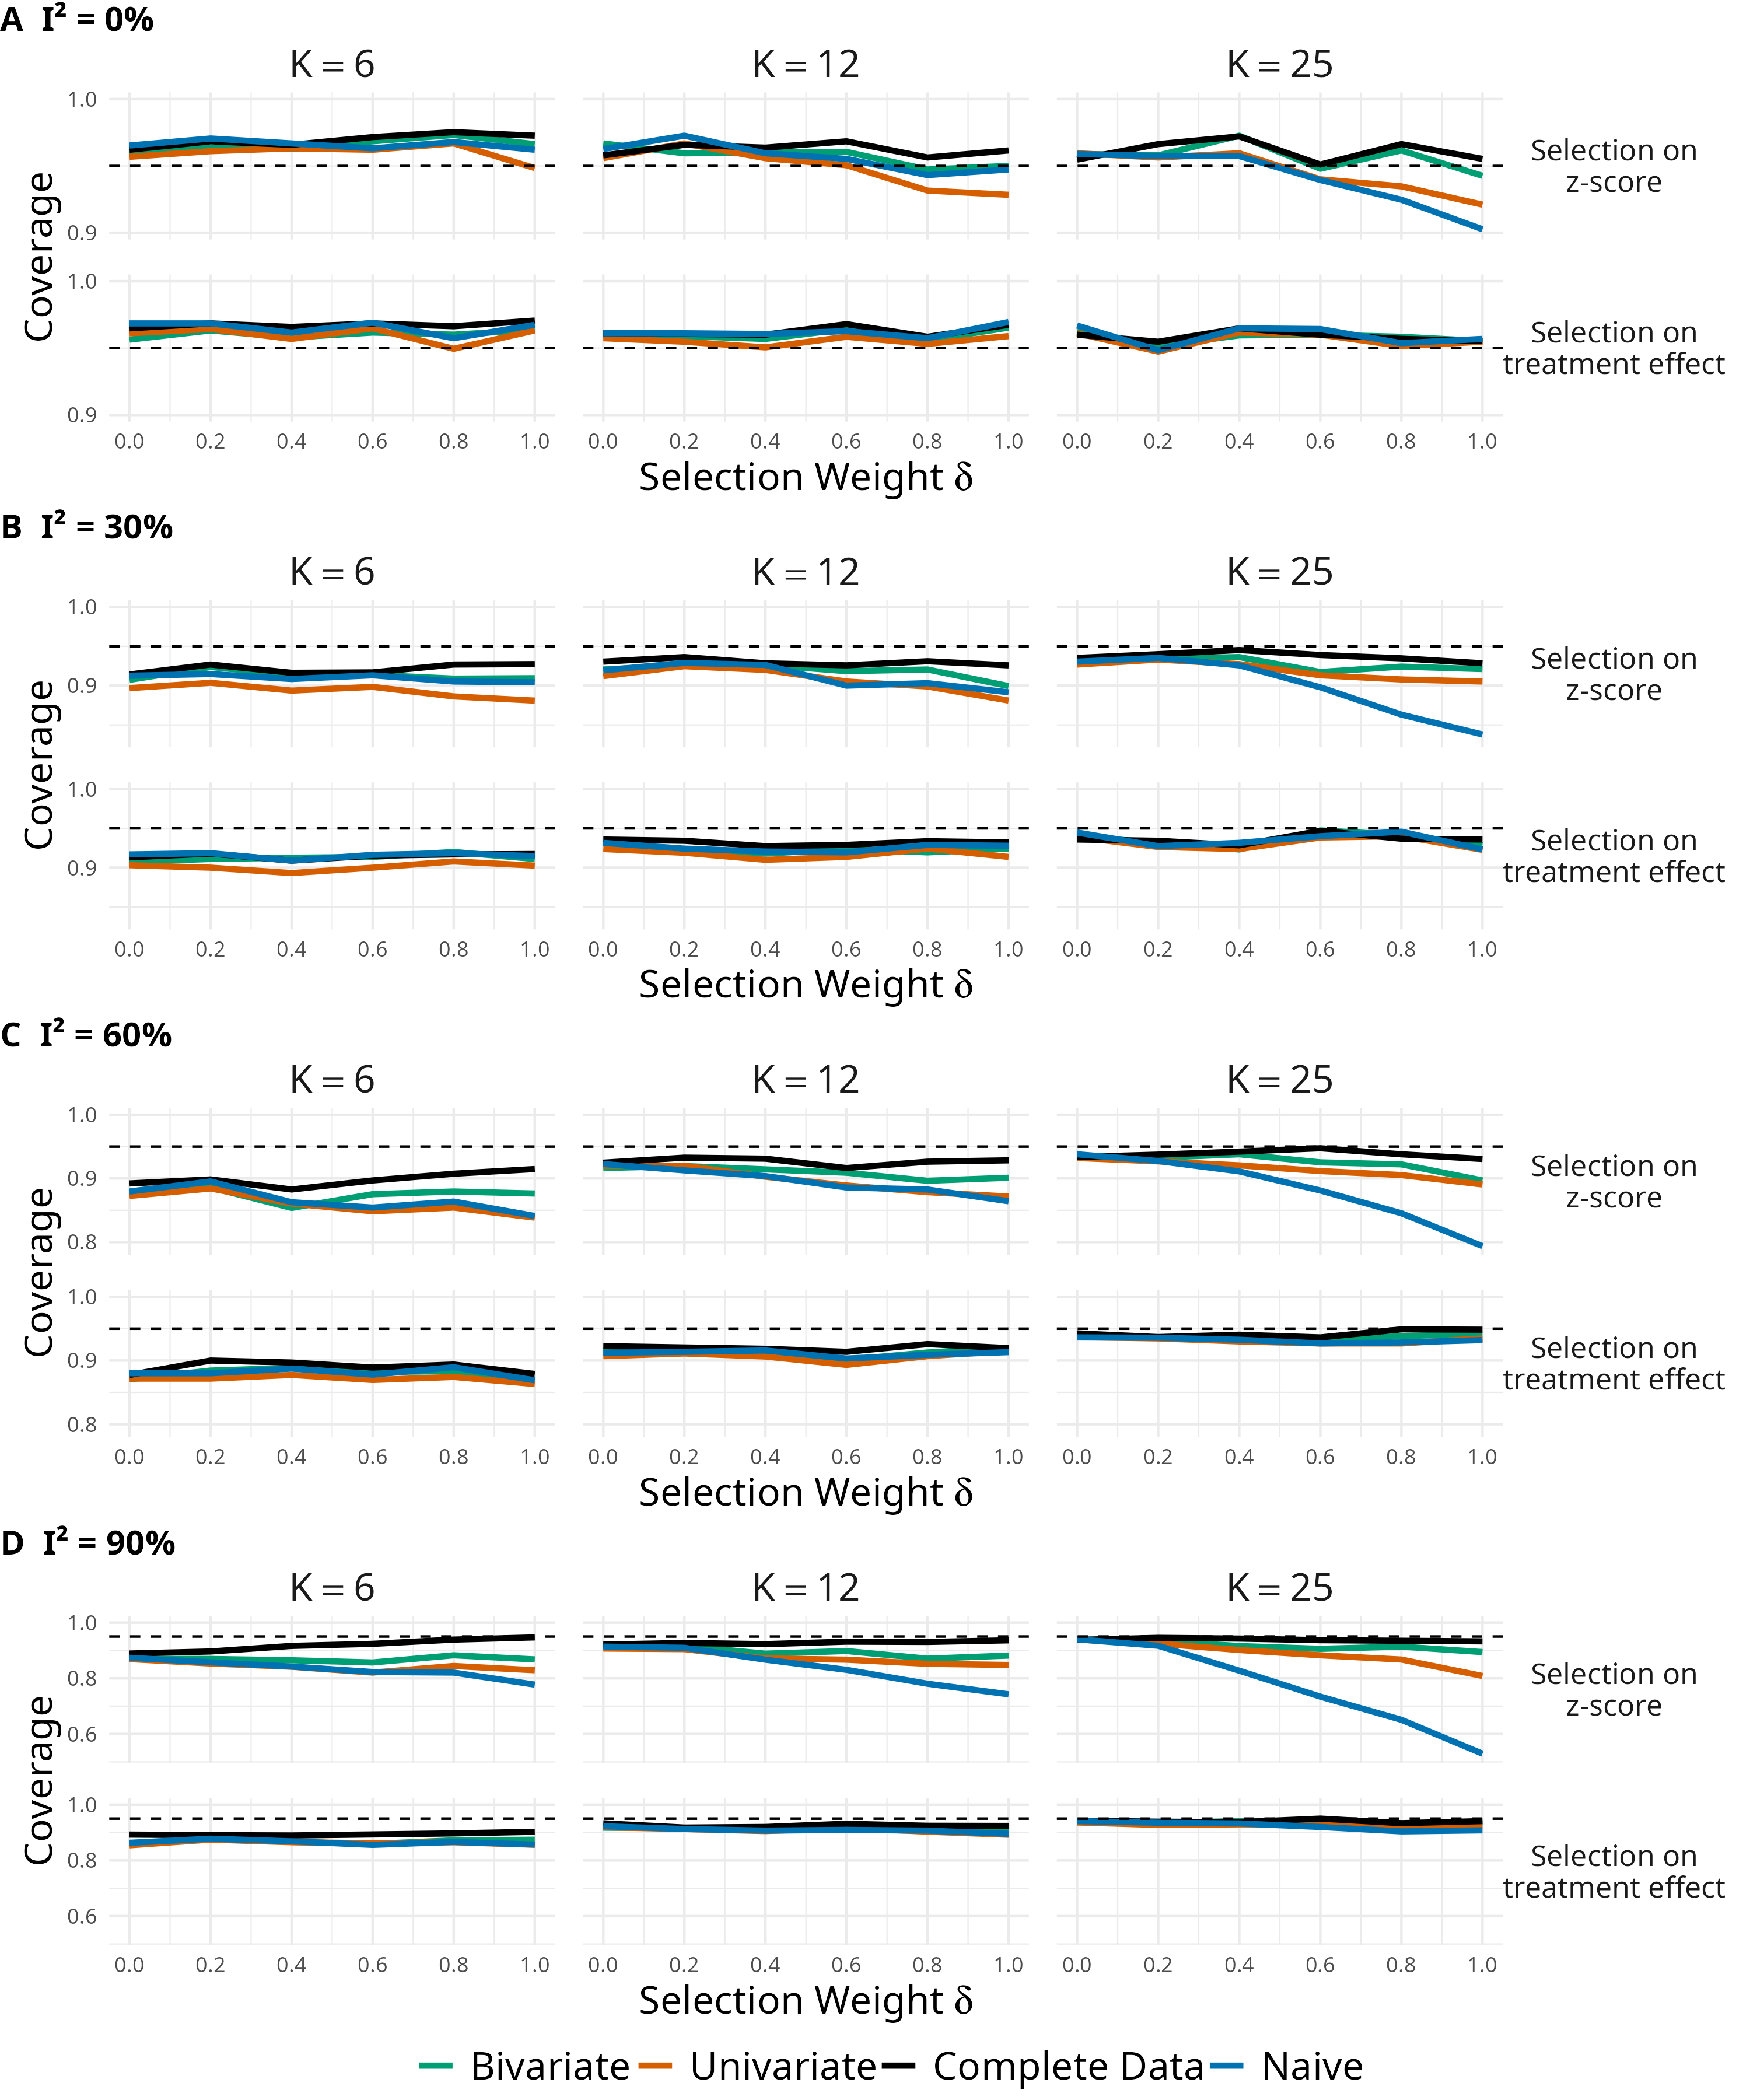
\includegraphics[width = 1\linewidth]{figures/Supp_SimStudy_Coverage_het.png}
\end{figure}

\clearpage


\subsection{Model misspecification for main scenario} 
\label{Misspecification}
In the manuscript’s results section of the simulation study, we focus on scenarios where $\delta_{1,\text{sim}} = \delta_{1,\text{est}}$. This supplementary document presents additional results from the simulation study for $\delta_{1,\text{sim}} \neq \delta_{1,\text{est}}$. 

The naive estimate exhibits the largest bias across nearly all scenarios (see Figure \ref{fig:App_Bias}). For both the univariate and bivariate ORB-adjusted estimates, bias generally increases as the assumed selection parameter $\delta_{1,\text{est}}$ deviates from the generating value $\delta_{1,\text{sim}}=0.8$, reflecting the impact of misspecifying the reporting mechanism. This effect is most pronounced under high heterogeneity (see Figure \ref{fig:App_Bias} D). As in the main simulation results, bias is larger under selection on the $z$-score than under selection on the treatment effect. Varying study sizes have comparatively little influence on the magnitude of bias.

The MSE is also highest for the naive estimate and decreases over increasing sample size (see Figure \ref{fig:App_MSE}). Although both adjusted estimates exhibit increased MSE under stronger misspecification, their MSE remains substantially lower than that of the naive estimate. Differences between the univariate and bivariate ORB-adjusted estimates are generally small, indicating that both approaches remain reasonably robust to moderate misspecification of the selection parameter.


\begin{figure}[!ht]
\centering
\caption{Simulation results for bias of four MA estimates of the treatment effect for outcome 1 under ORB and model misspecification for $\theta_1 = \theta_2 = 0.4$, $\rho_B = \rho_W = 0.8$, $p_1 = 20\%$ and $\delta_{1,\text{sim}} = 0.8$. Results are shown for varying numbers of studies, heterogeneity levels, selection type, and an increasing selection parameter.}
\label{fig:App_Bias}
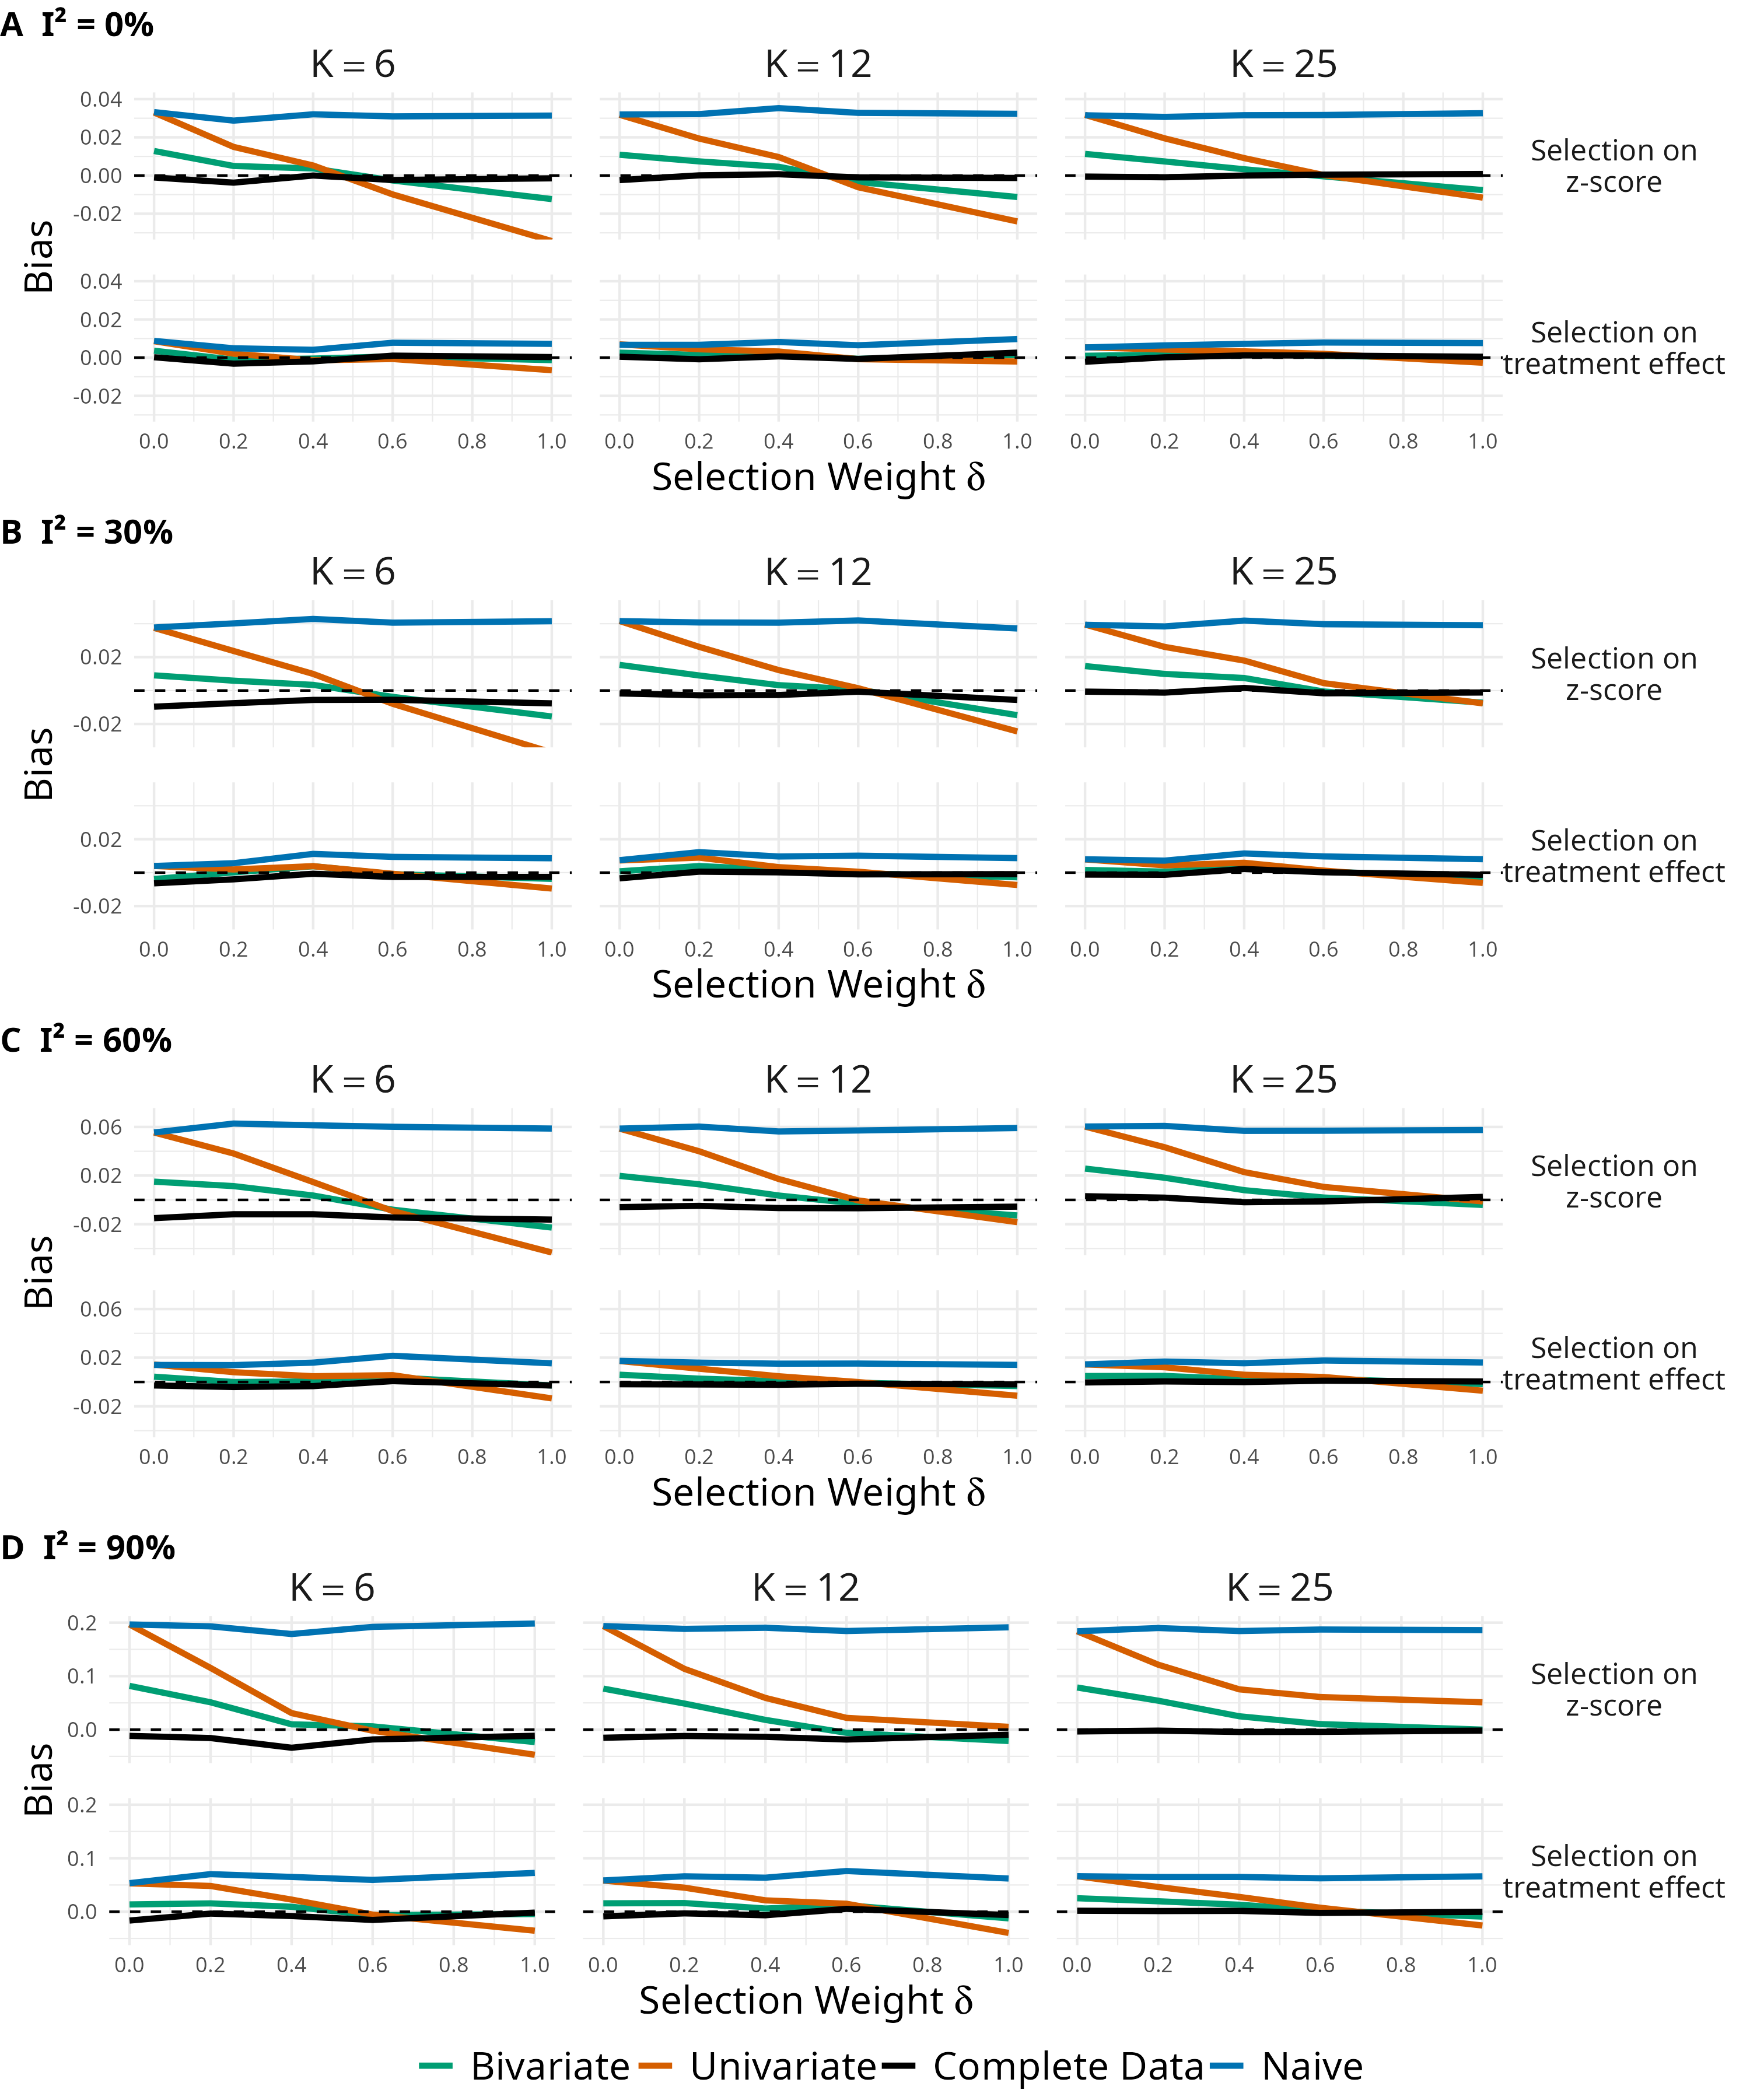
\includegraphics[width = 1\linewidth]{figures/Supp_SimStudy_Bias.png}
\end{figure}

\begin{figure}[!ht]
\centering
\caption{Simulation results for MSE of four MA estimates of the treatment effect for outcome 1 under ORB and model misspecification for $\theta_1 = \theta_2 = 0.4$, $\rho_B = \rho_W = 0.8$, $p_1 = 20\%$ and $\delta_{1,\text{sim}} = 0.8$. Results are shown for varying numbers of studies, heterogeneity levels, selection type, and an increasing selection parameter.}
\label{fig:App_MSE}
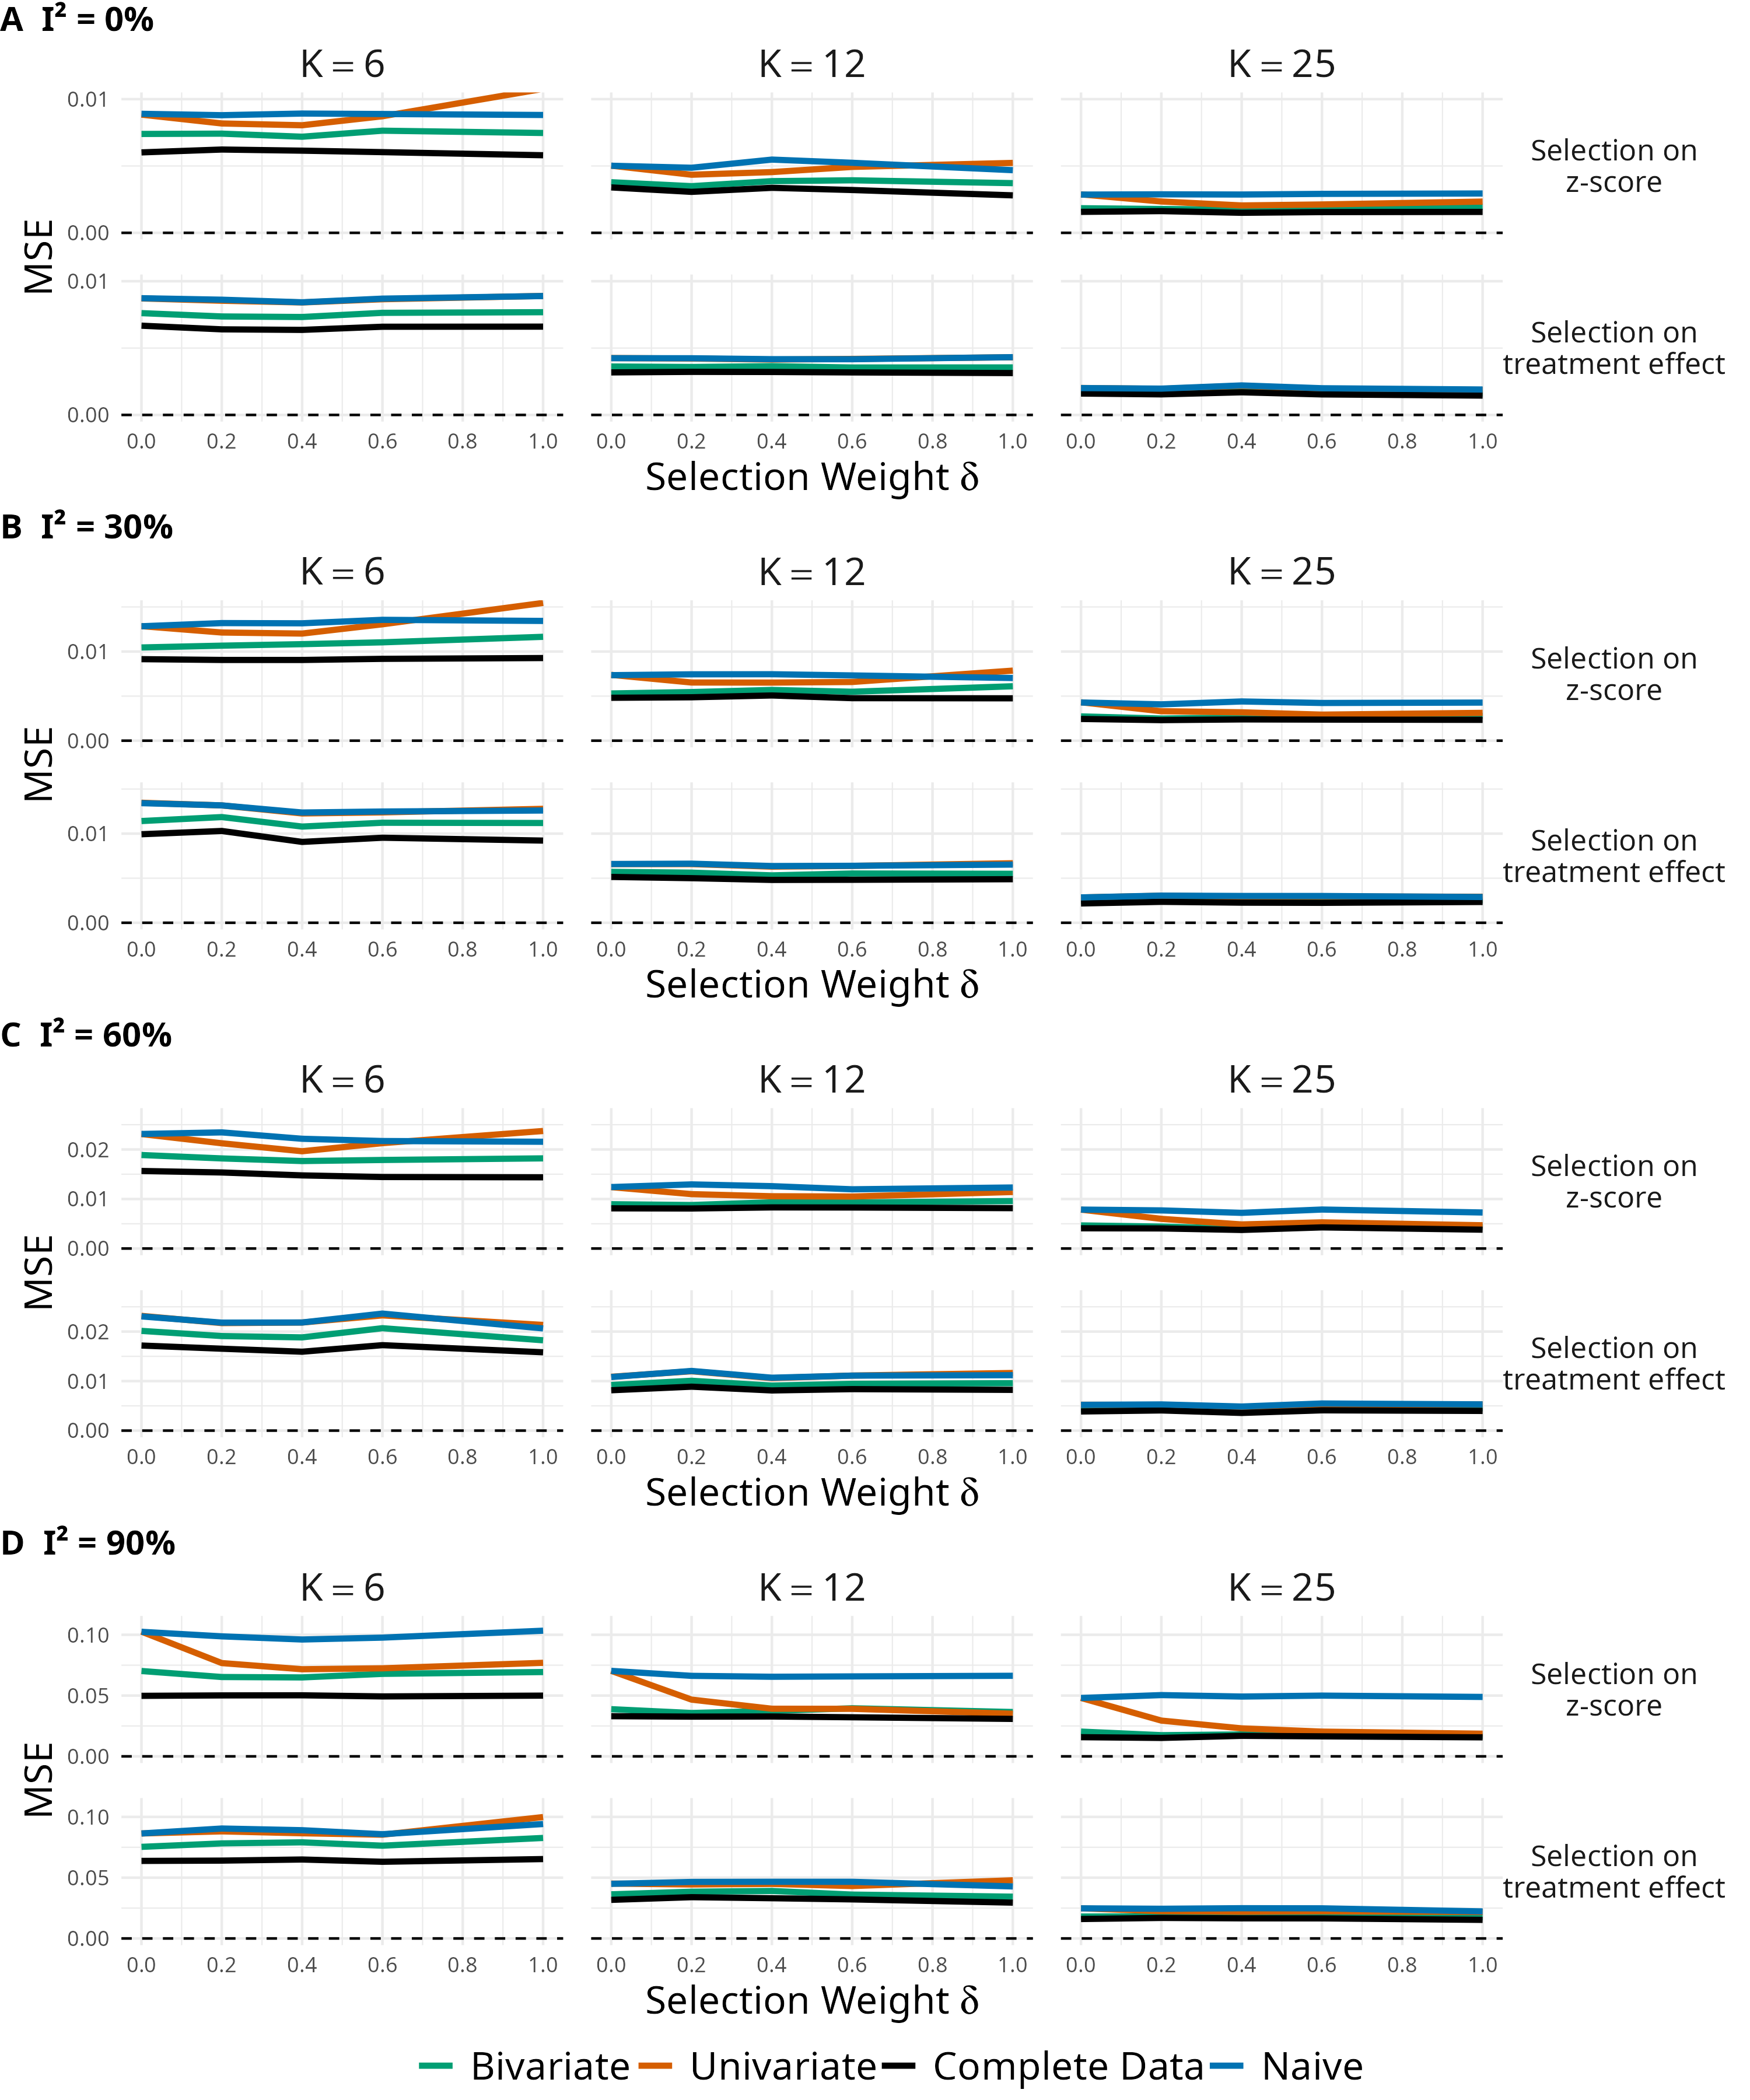
\includegraphics[width = 1\linewidth]{figures/Supp_SimStudy_MSE.png}
\end{figure}

CI width decreases as the number of studies increases, reflecting improved estimation precision. For all scenarios except for high heterogeneity ($I^2 = 90\%$), the complete data estimate has the lowest CI width. For high heterogeneity the univariate ORB-adjusted estimate has the lowest CI width, reflecting differences in the weighting and imputation procedures under severe selective reporting (see Figure \ref{fig:App_CI} D).


\begin{figure}[!ht]
\centering
\caption{Simulation results for CI width of four MA estimates of the treatment effect for outcome 1 under ORB and model misspecification for $\theta_1 = \theta_2 = 0.8$, $\rho_B = \rho_W = 0.4$, $p_1 = 20\%$ and $\delta_{1,\text{sim}} = 0.8$. Results are shown for varying numbers of studies, heterogeneity levels, selection type, and an increasing selection parameter.}
\label{fig:App_CI}
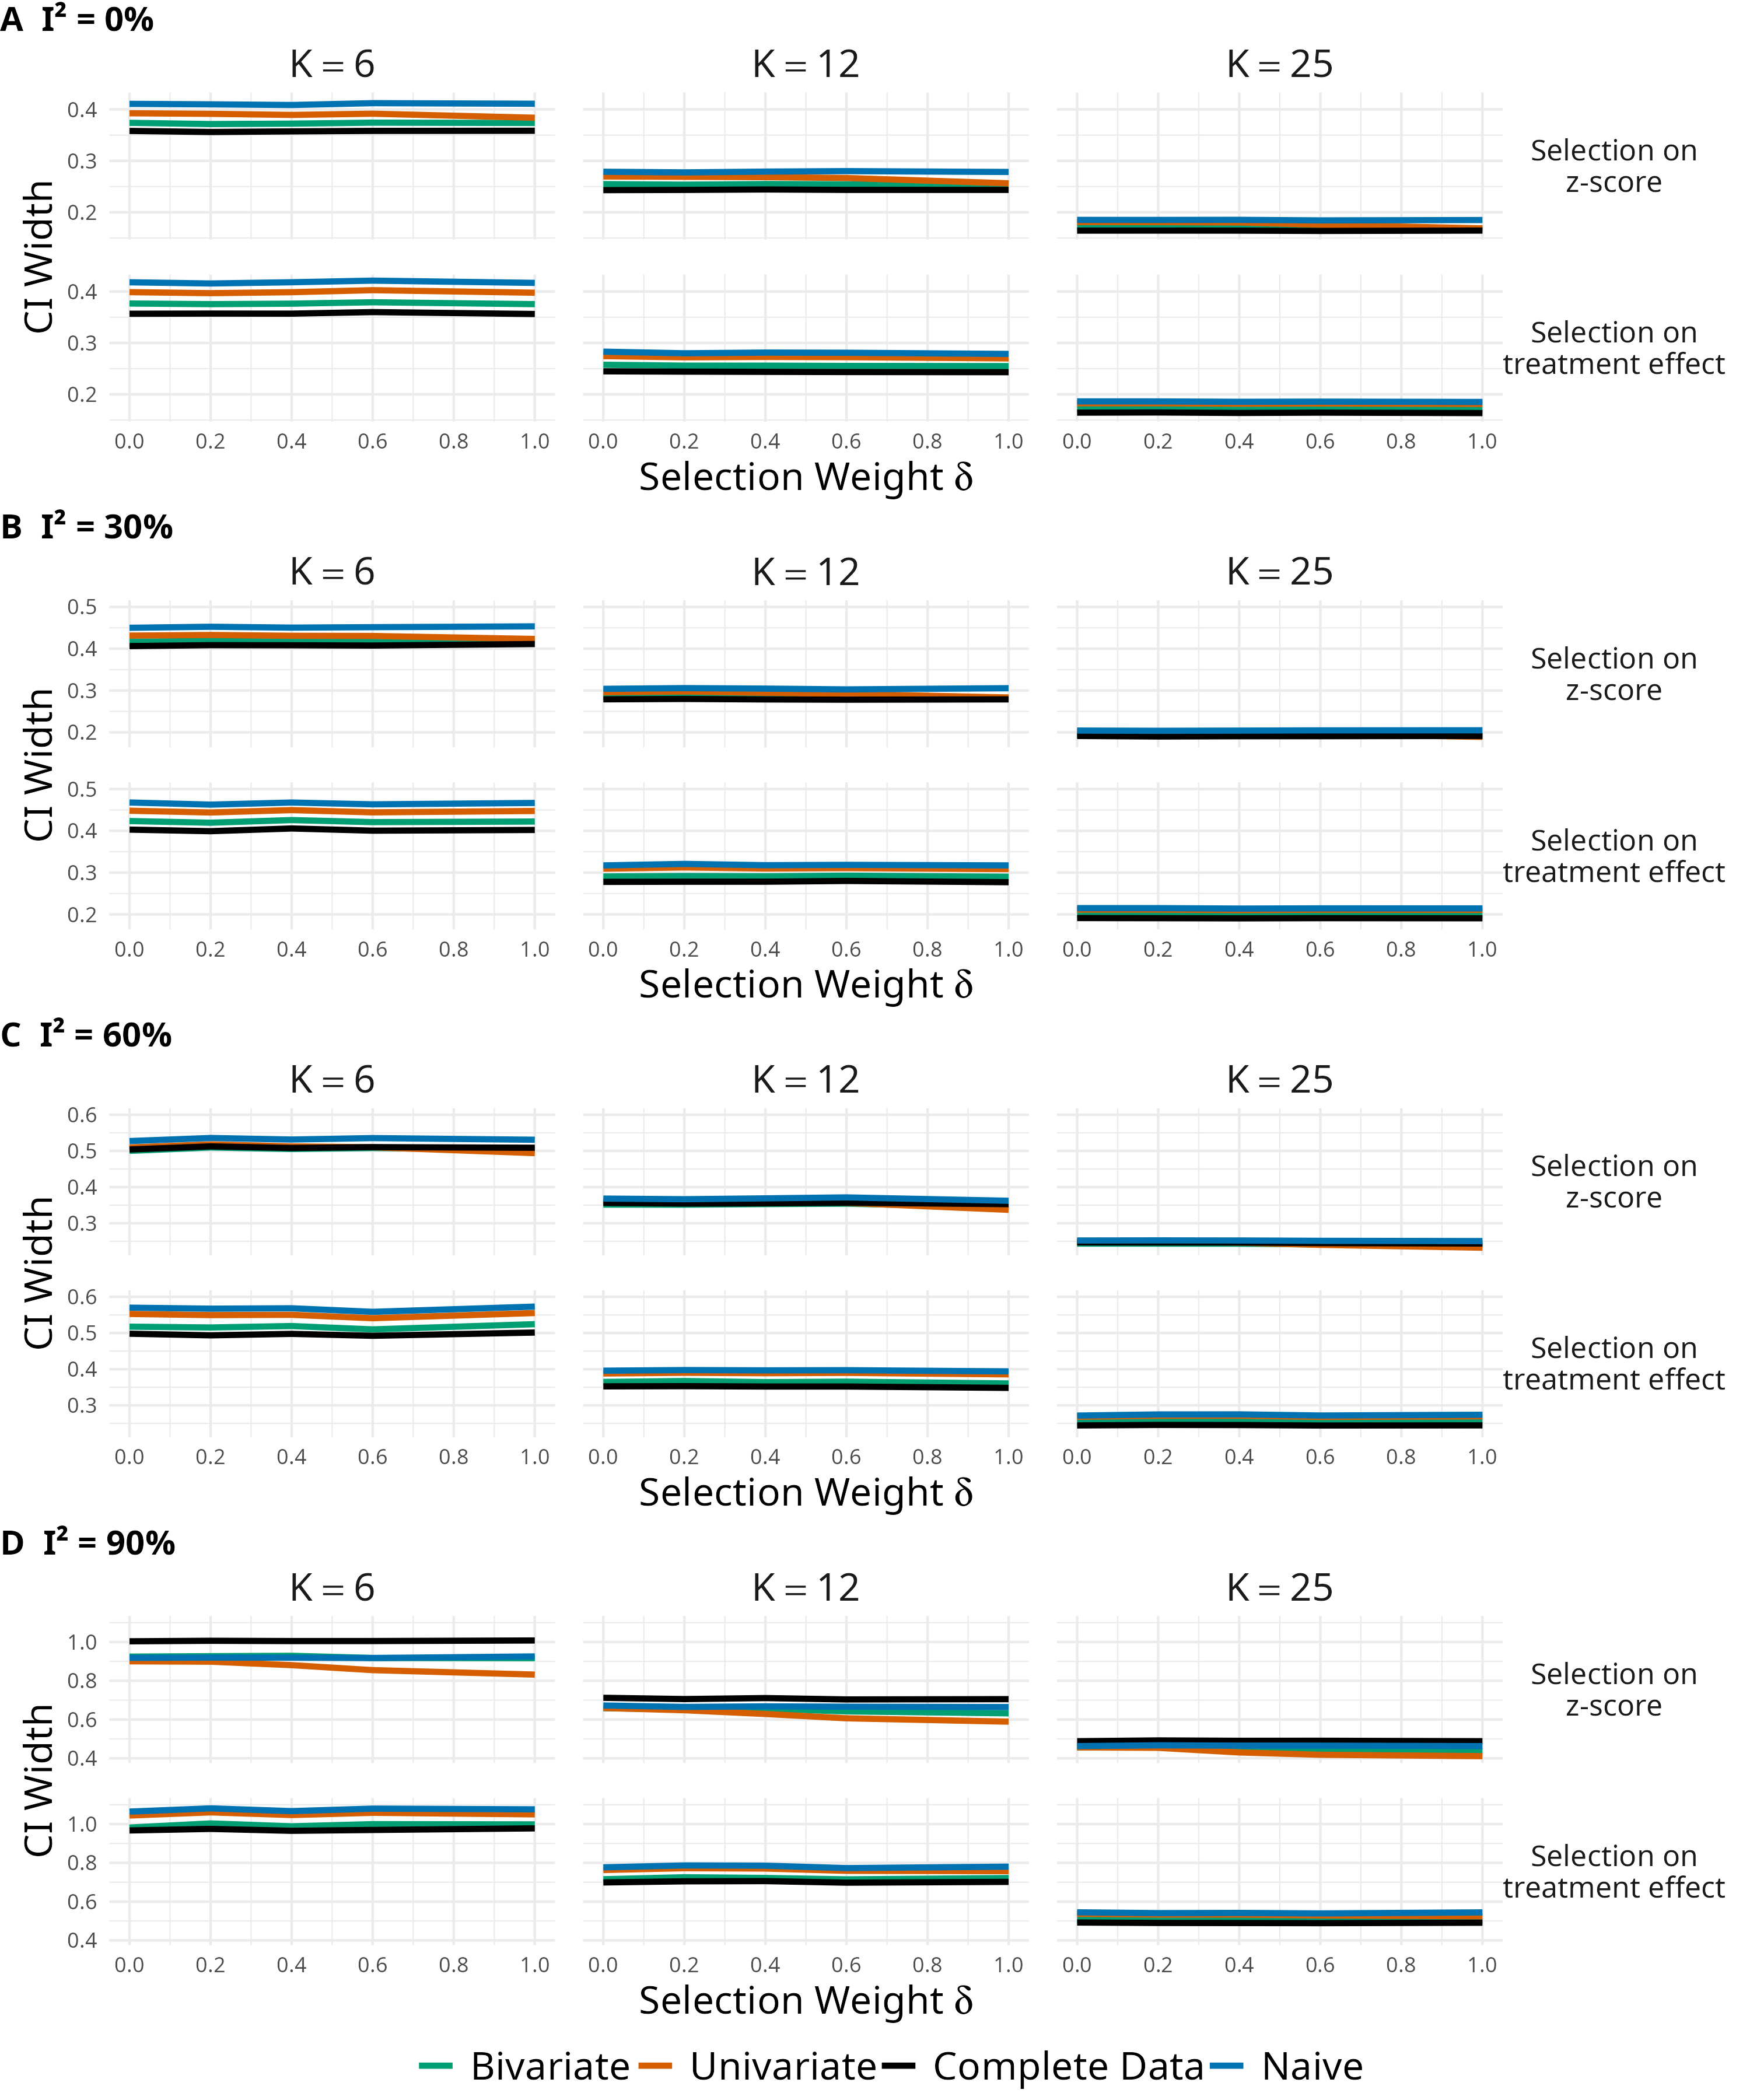
\includegraphics[width = 1\linewidth]{figures/Supp_SimStudy_CIWidth.png}
\end{figure}


As expected, the complete estimate maintains also for model misspecification nominal coverage at approximately 95\% across all simulated scenarios, serving as a reference baseline. The naive estimate shows acceptable nominal coverage when heterogeneity is low to moderate ($I^2 \le 60\%$). However, under strong heterogeneity ($I^2 = 90\%$), its performance degrades as the estimation selection weight increases. Particularly for large sample sizes ($K = 25$) under $z$-score selection coverage drops below 70\% (see Figure \ref{fig:App_Cov} D). The bivariate ORB-adjusted estimate demonstrates robust recovery of the nominal coverage probability across most scenarios. Under extreme heterogeneity ($I^2 = 90\%$), it exhibits a slight drop in coverage at lower estimation selection weights ($\delta = 0$) when the estimation model undercorrects for bias. However, it quickly converges toward nominal coverage as the estimated selection weight approaches the generating parameter ($\delta_{\text{sim}} = 0.8$). The univariate adjusted method underperforms compared to the bivariate model, particularly under high heterogeneity ($I^2 \ge 60\%$) and when the estimated selection weight is low (see Figure \ref{fig:App_Cov}). This under-coverage may arise from a combination of residual variance underestimation and reduced borrowing of strength compared to the bivariate approach. Overall, the additional analyses demonstrate that both ORB-adjusted methods have substantial advantages over the naive estimate even when the selection mechanism is misspecified.


\begin{figure}[!ht]
\centering
\caption{Simulation results for coverage of four MA estimates of the treatment effect for outcome 1 under ORB and model misspecification for $\theta_1 = \theta_2 = 0.4$, $\rho_B = \rho_W = 0.8$, $p_1 = 20\%$ and $\delta_{1,\text{sim}} = 0.8$. Results are shown for varying numbers of studies, heterogeneity levels, selection type, and an increasing selection parameter.}
\label{fig:App_Cov}
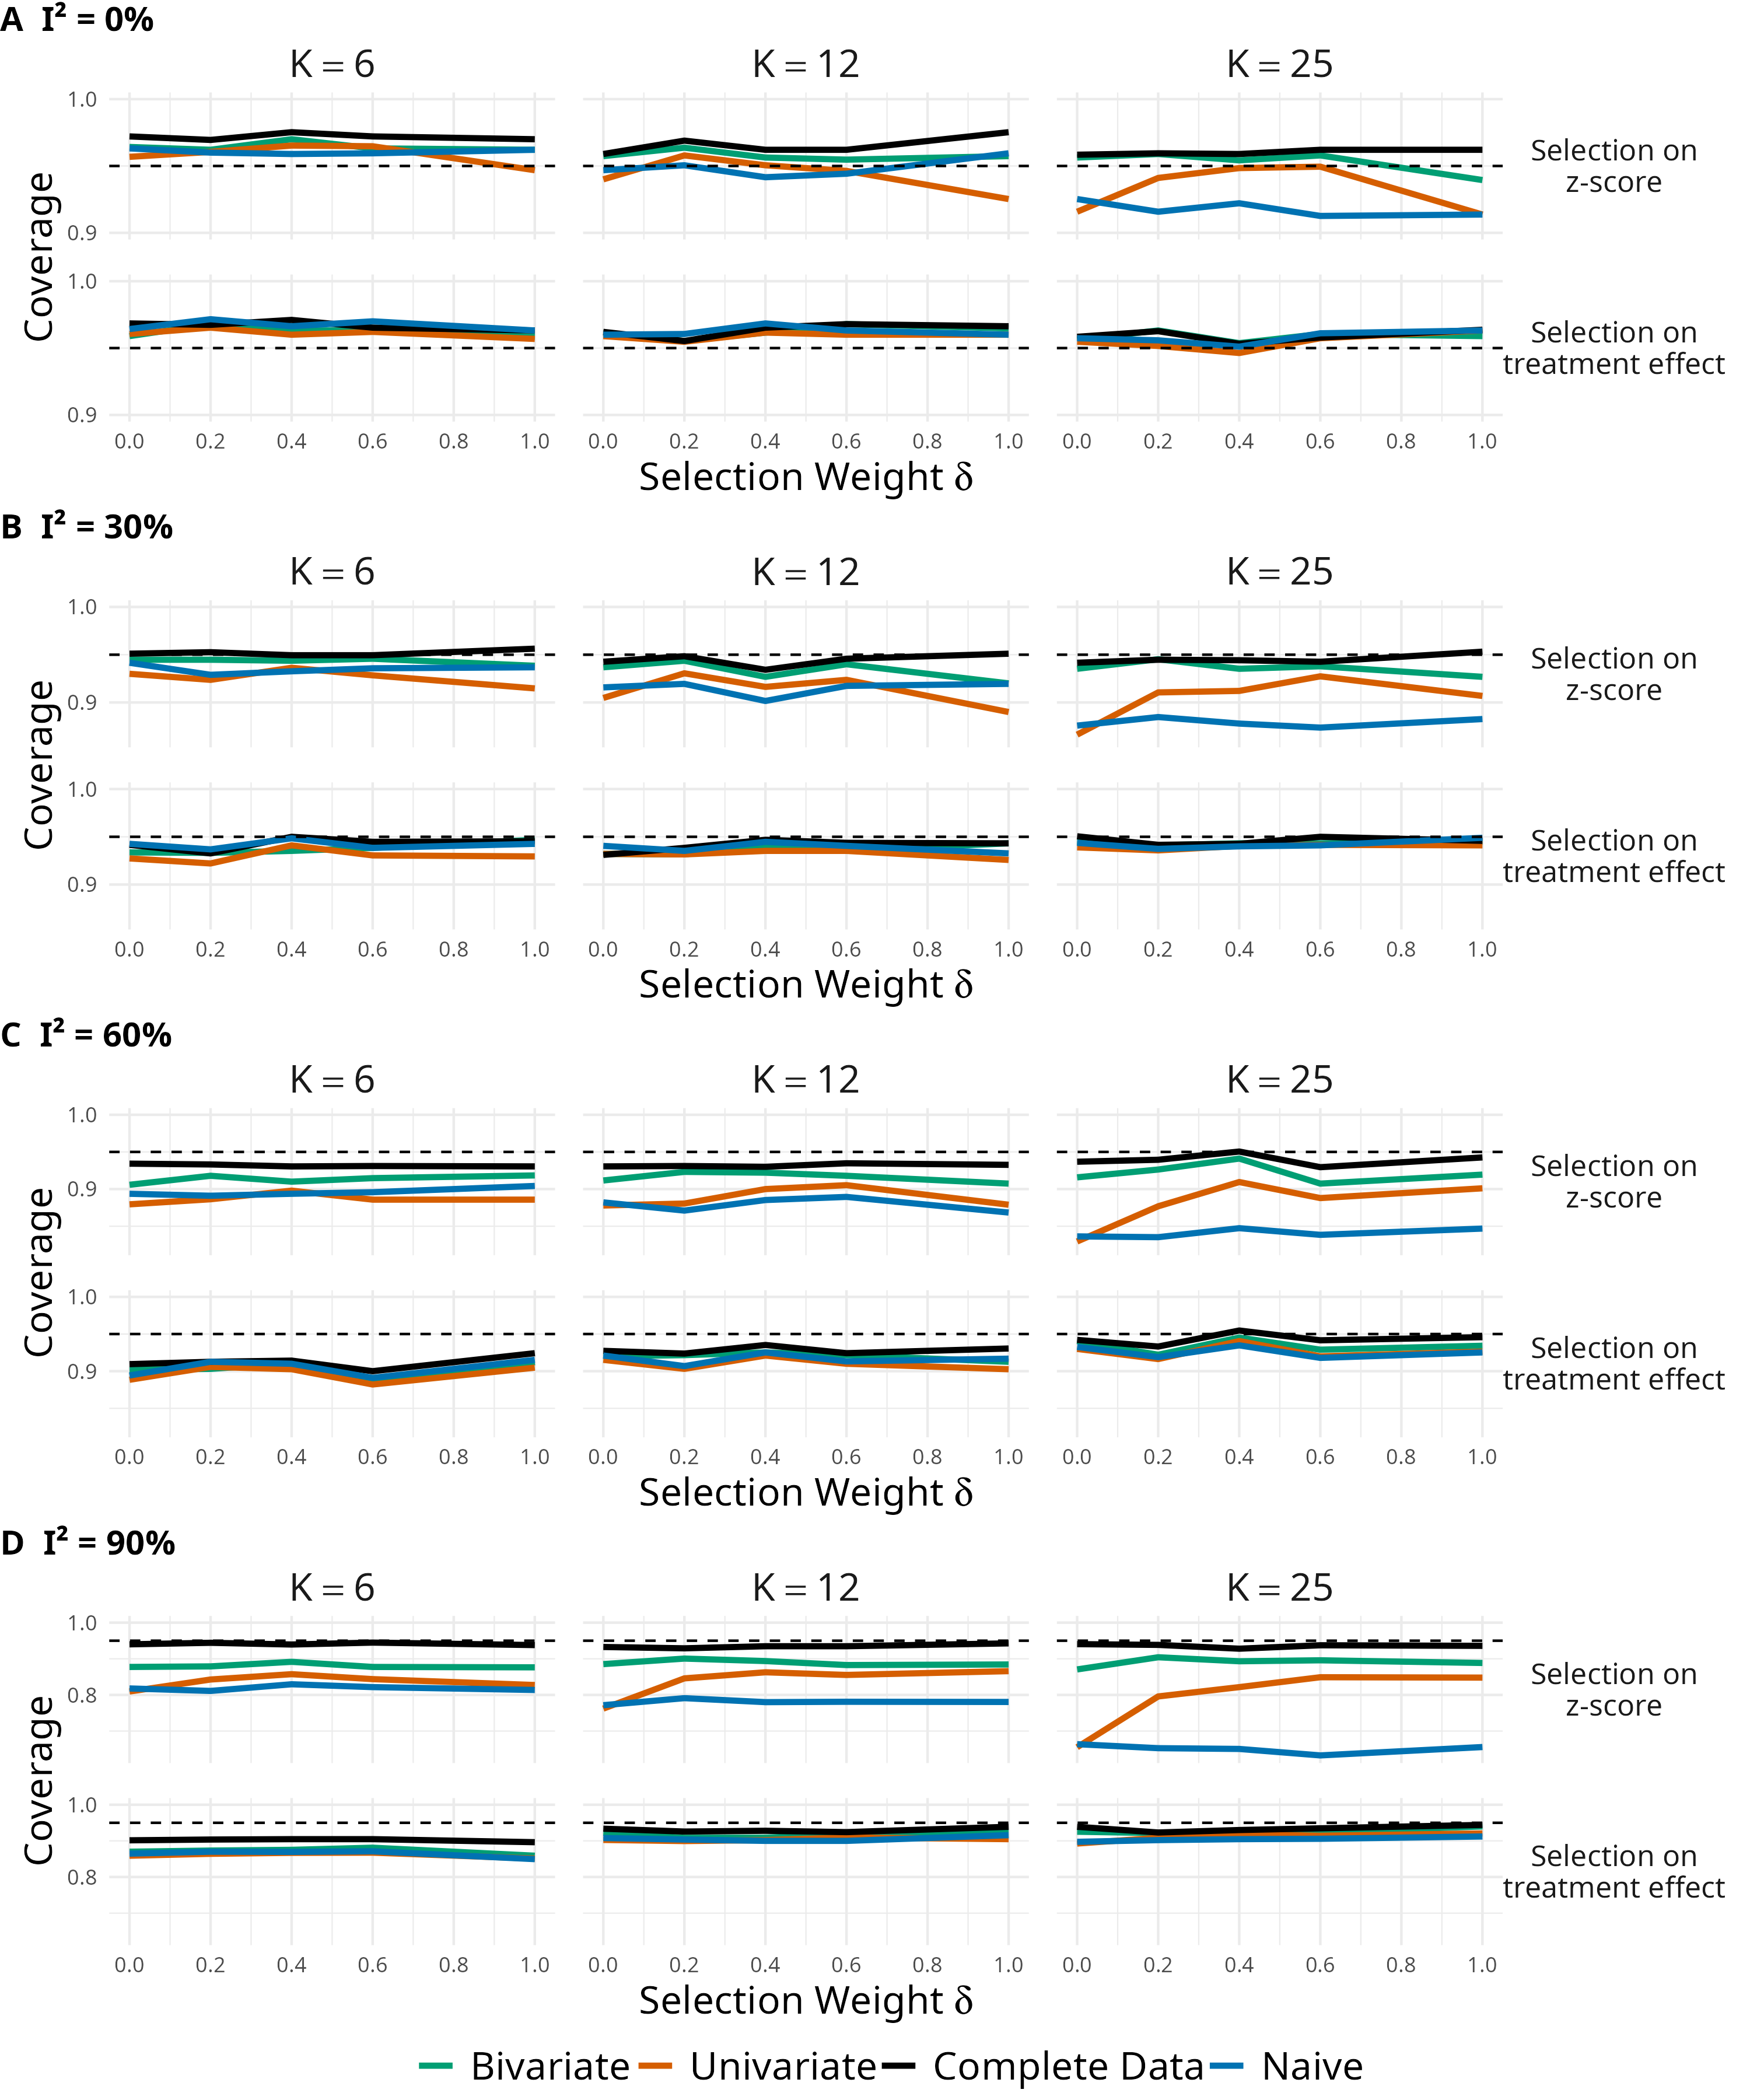
\includegraphics[width = 1\linewidth]{figures/Supp_SimStudy_Coverage.png}
\end{figure}

\clearpage

\subsection{\mycolor{Simulation scenario for $\theta_1 = \theta_2 = 0$}}

\begin{figure}[!ht]
\centering
\caption{Simulation results for bias of four MA estimates of the treatment effect for outcome 1 under ORB for $\theta_1 = \theta_2 = 0$, $\rho_B = \rho_W = 0.8$ and $p_1 = 20\%$. Results are shown for varying numbers of studies, heterogeneity levels, selection type, and an increasing selection parameter.}
\label{fig:App_Bias_theta0}
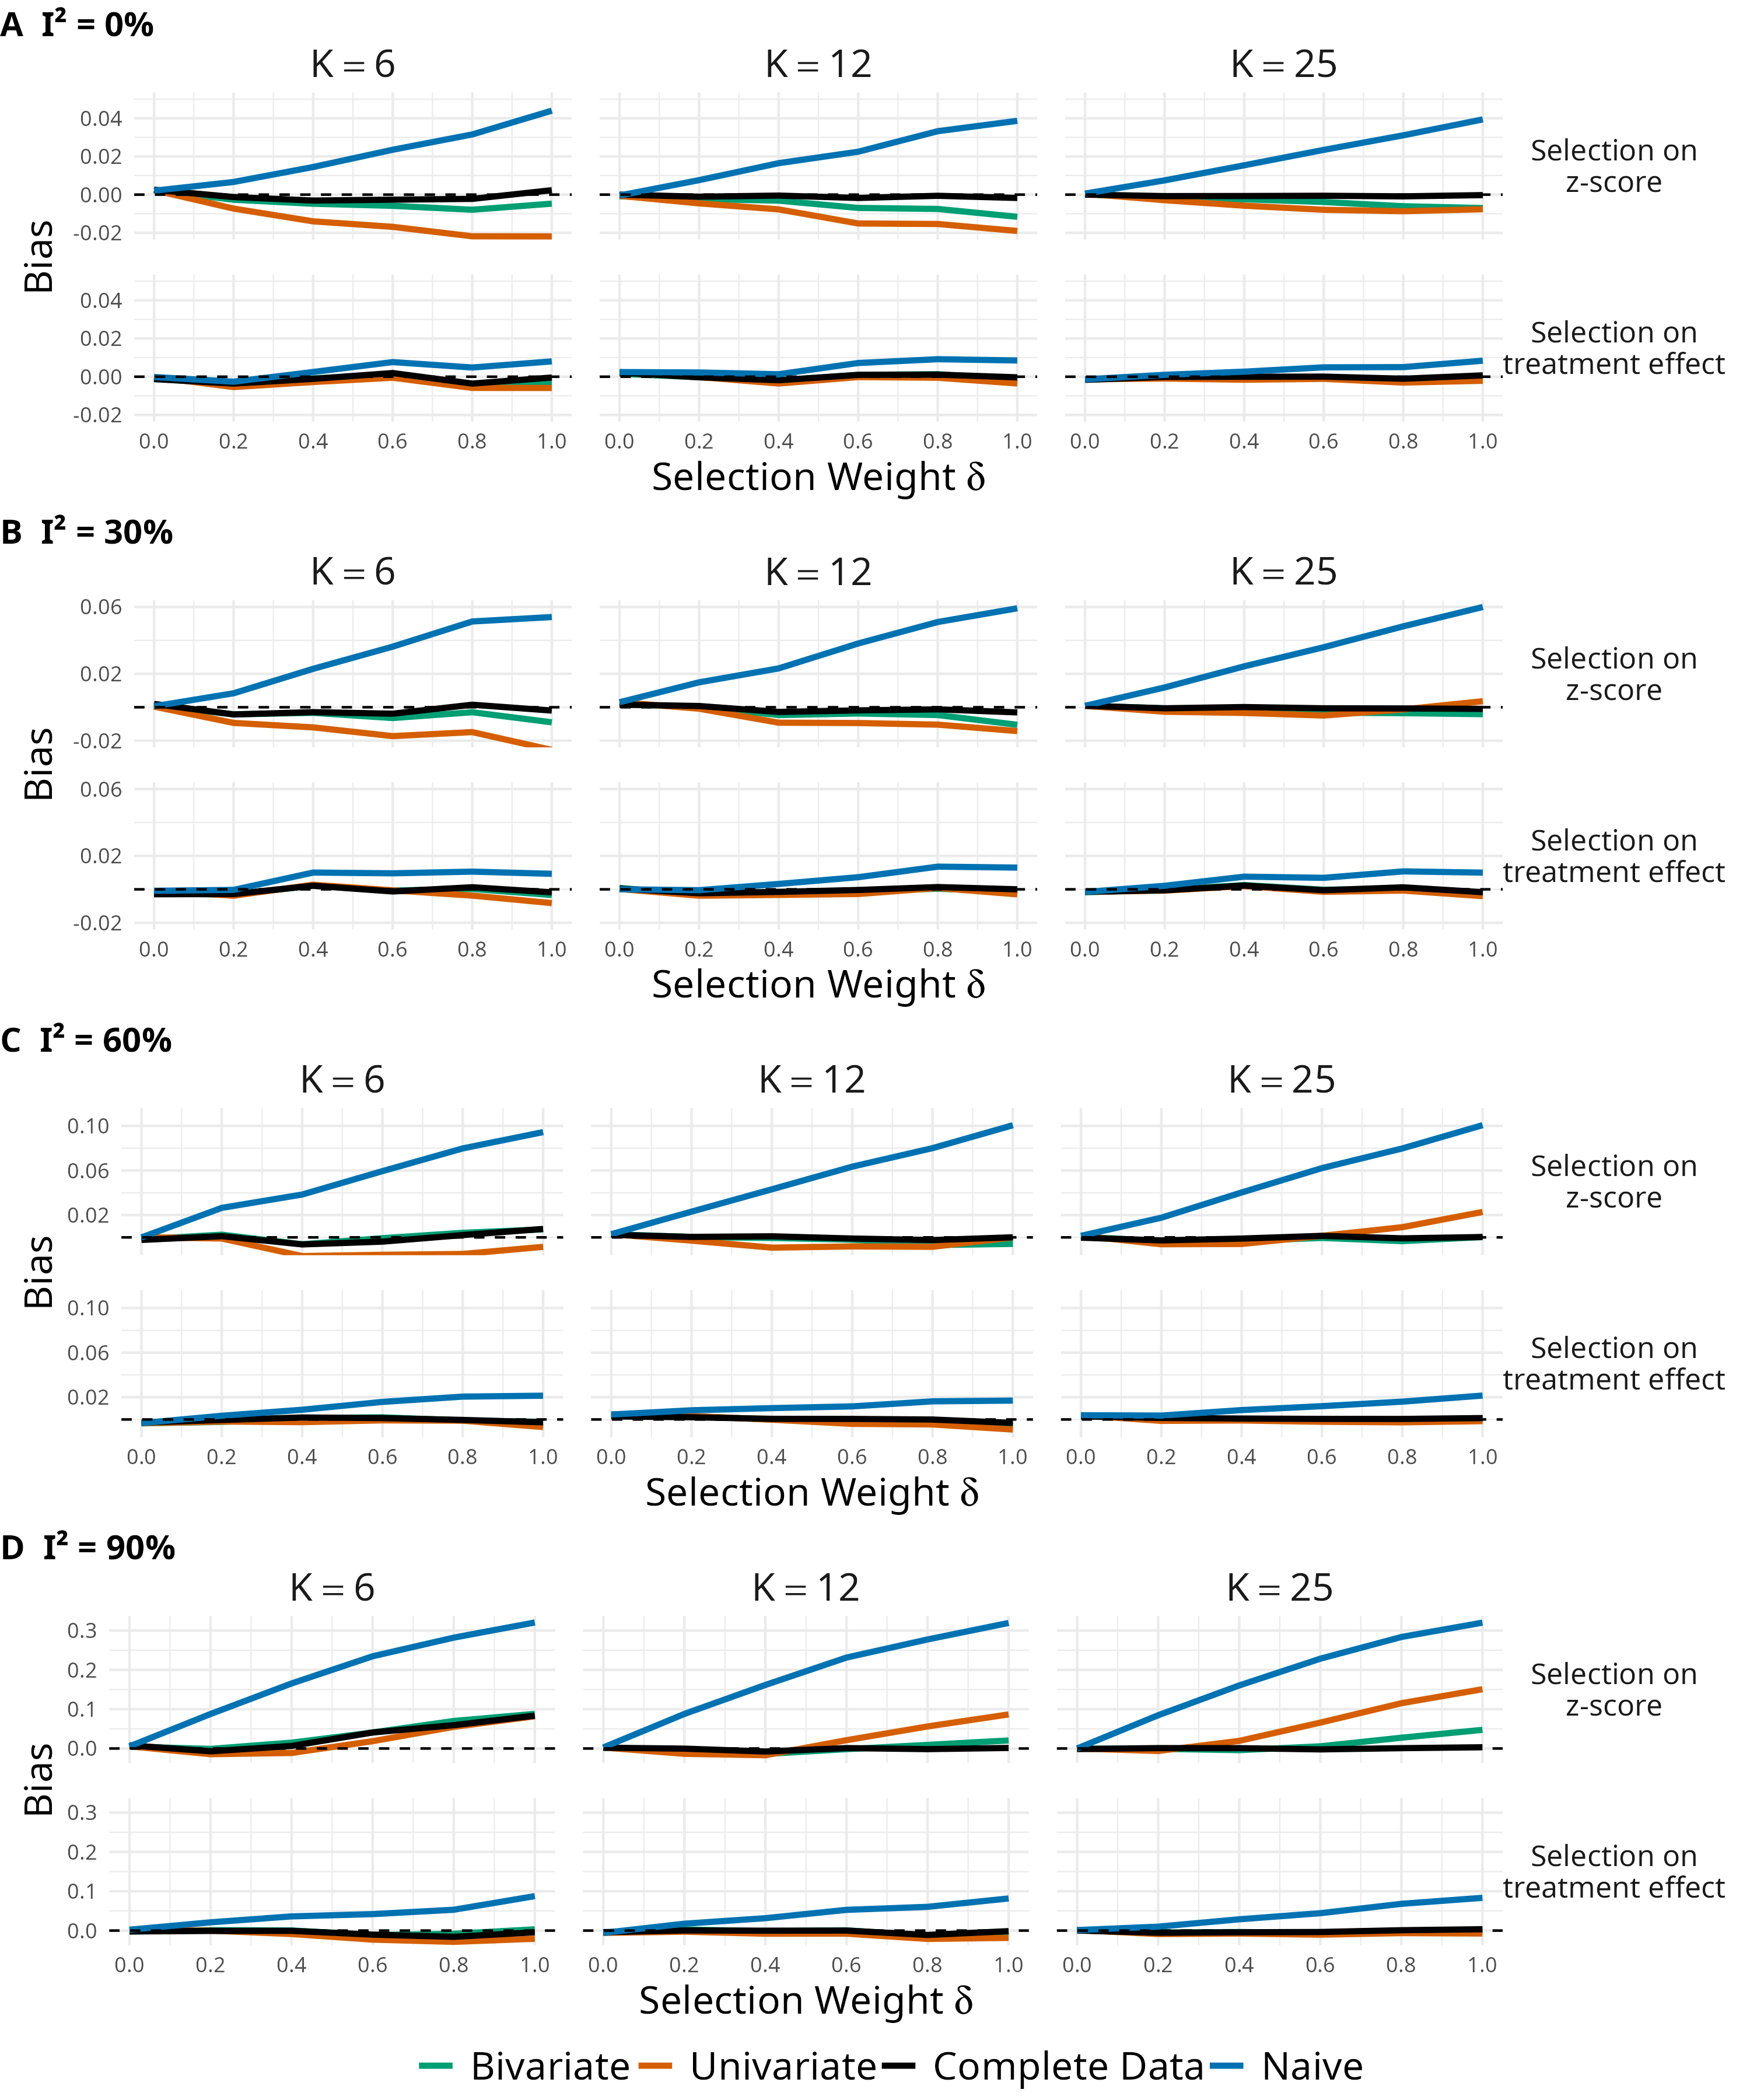
\includegraphics[width = 1\linewidth]{figures/Supp_SimStudy_Bias_theta0.png}
\end{figure}

\begin{figure}[!ht]
\centering
\caption{Simulation results for MSE of four MA estimates of the treatment effect for outcome 1 under ORB for $\theta_1 = \theta_2 = 0$, $\rho_B = \rho_W = 0.8$ and $p_1 = 20\%$. Results are shown for varying numbers of studies, heterogeneity levels, selection type, and an increasing selection parameter.}
\label{fig:App_MSE_theta0}
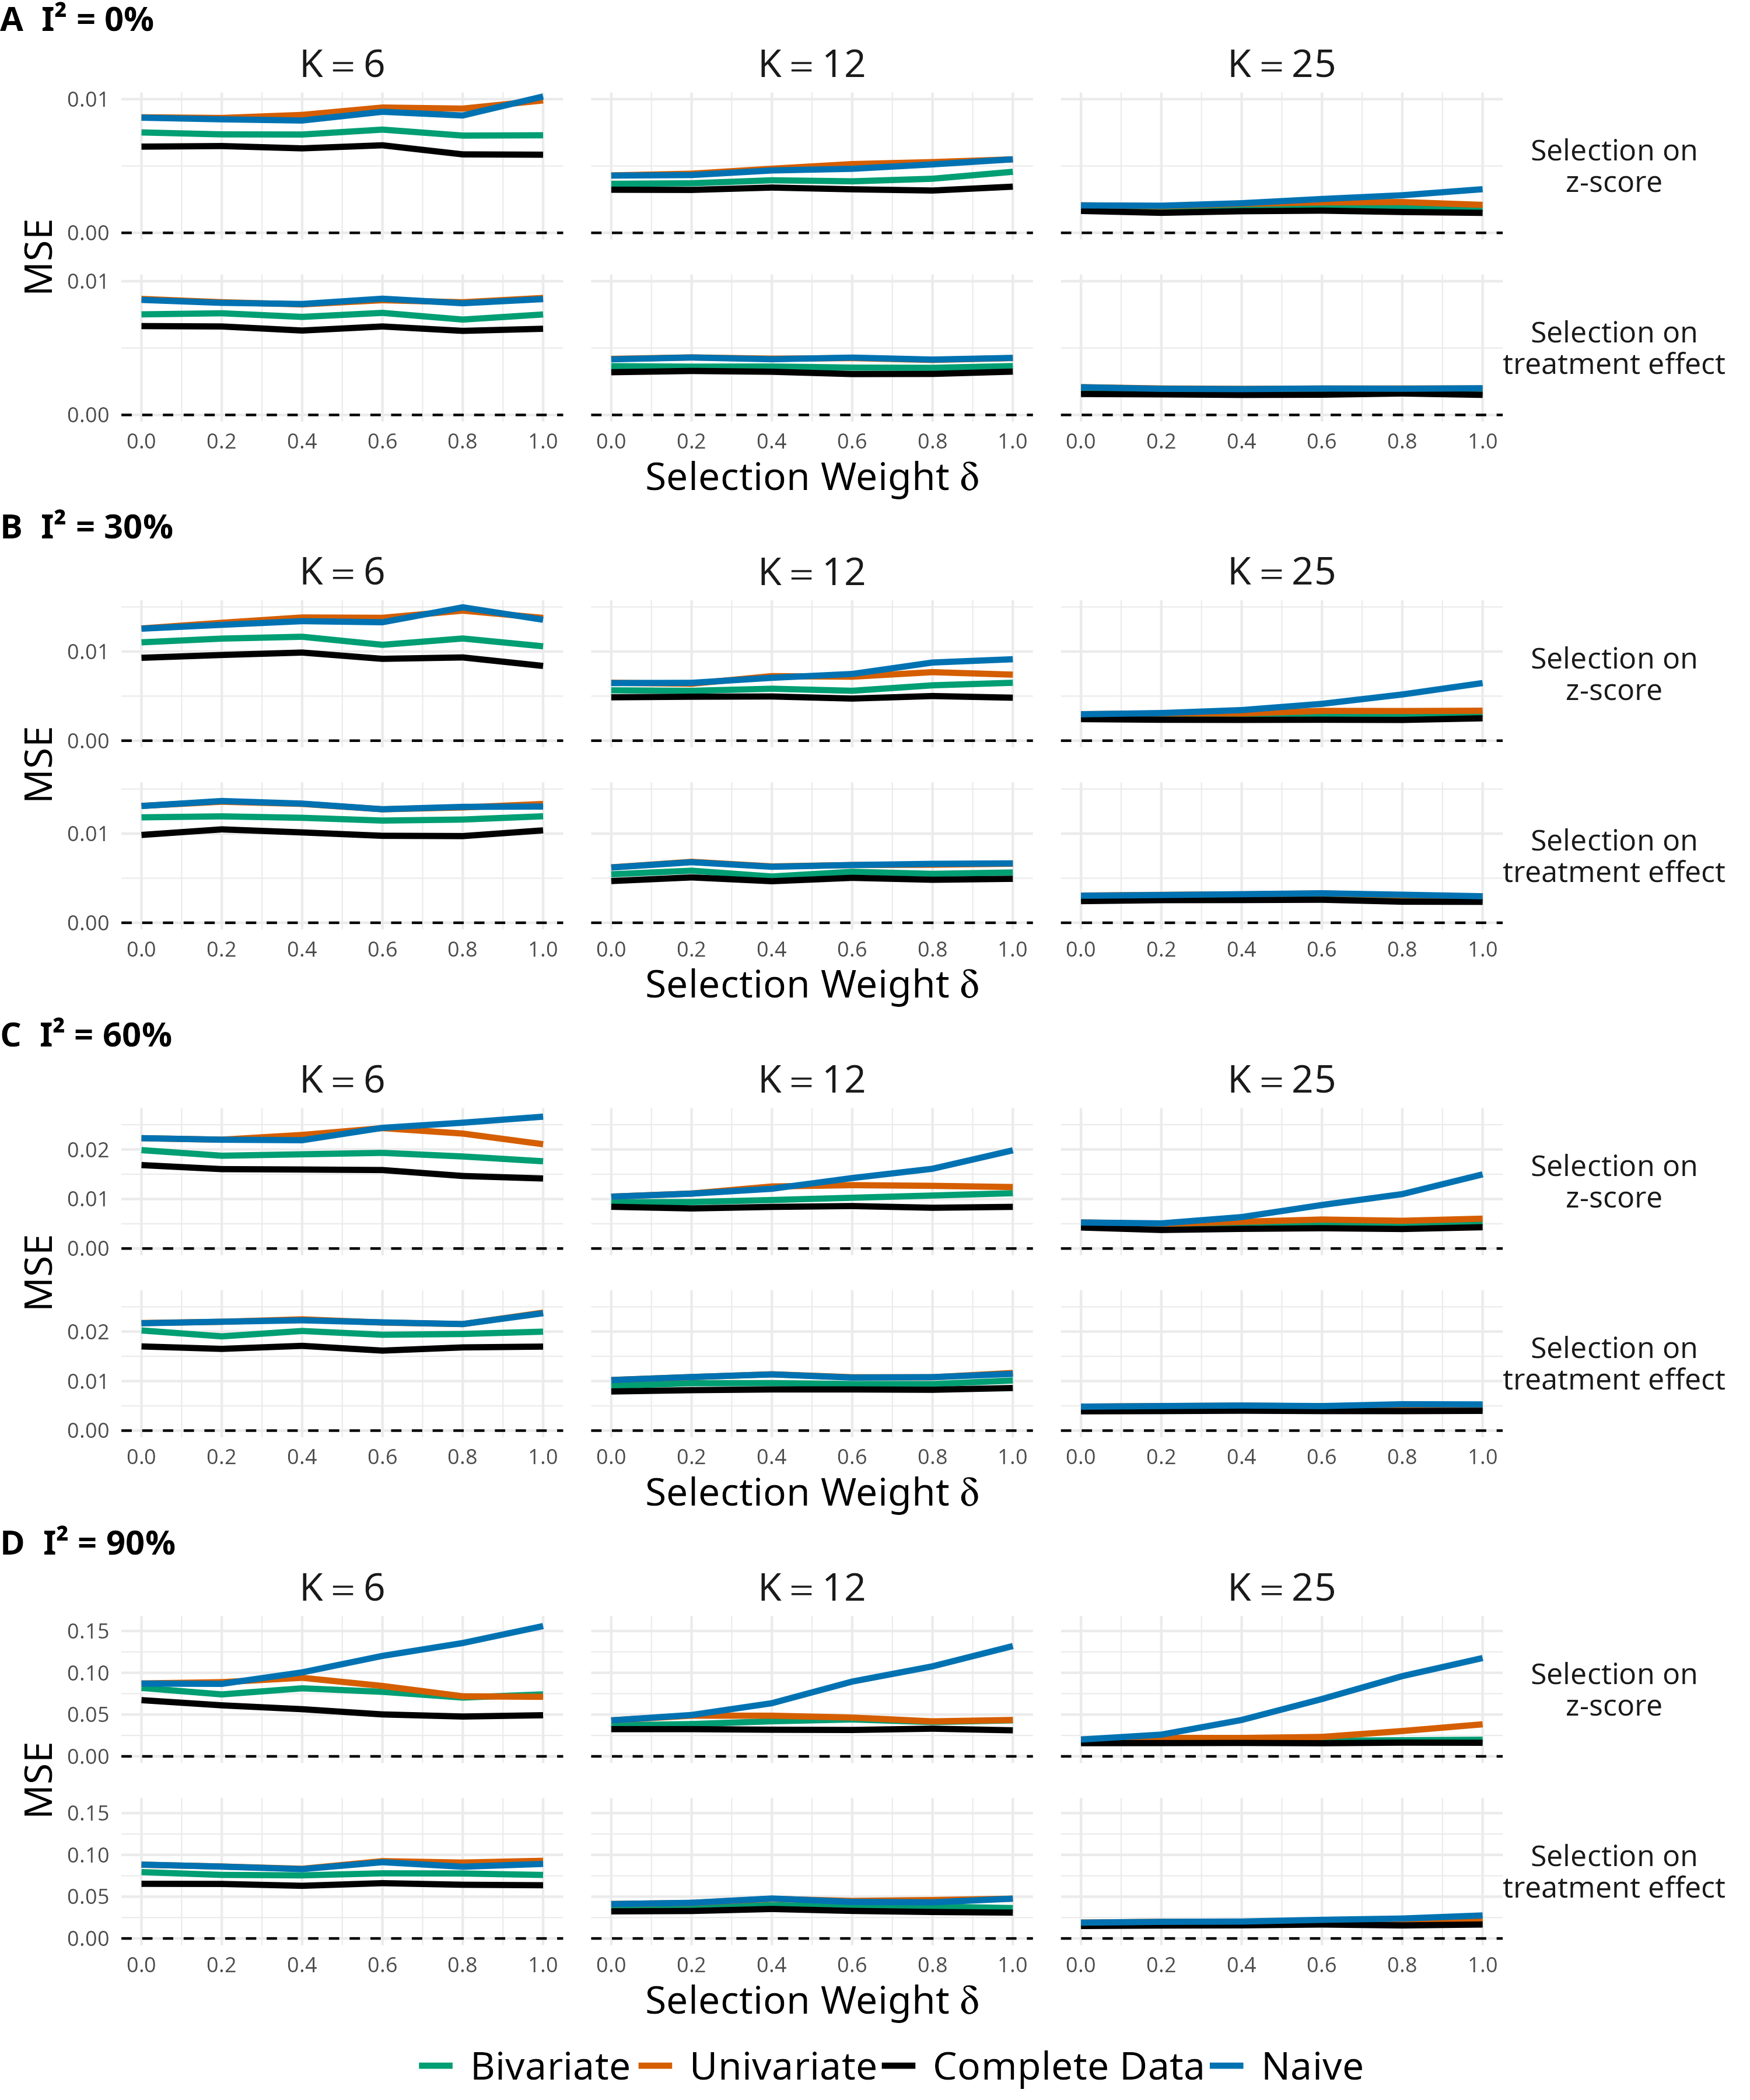
\includegraphics[width = 1\linewidth]{figures/Supp_SimStudy_MSE_theta0.png}
\end{figure}

\begin{figure}[!ht]
\centering
\caption{Simulation results for CI width of four MA estimates of the treatment effect for outcome 1 under ORB for $\theta_1 = \theta_2 = 0$, $\rho_B = \rho_W = 0.8$ and $p_1 = 20\%$. Results are shown for varying numbers of studies, heterogeneity levels, selection type, and an increasing selection parameter.}
\label{fig:App_CIWidth_theta0}
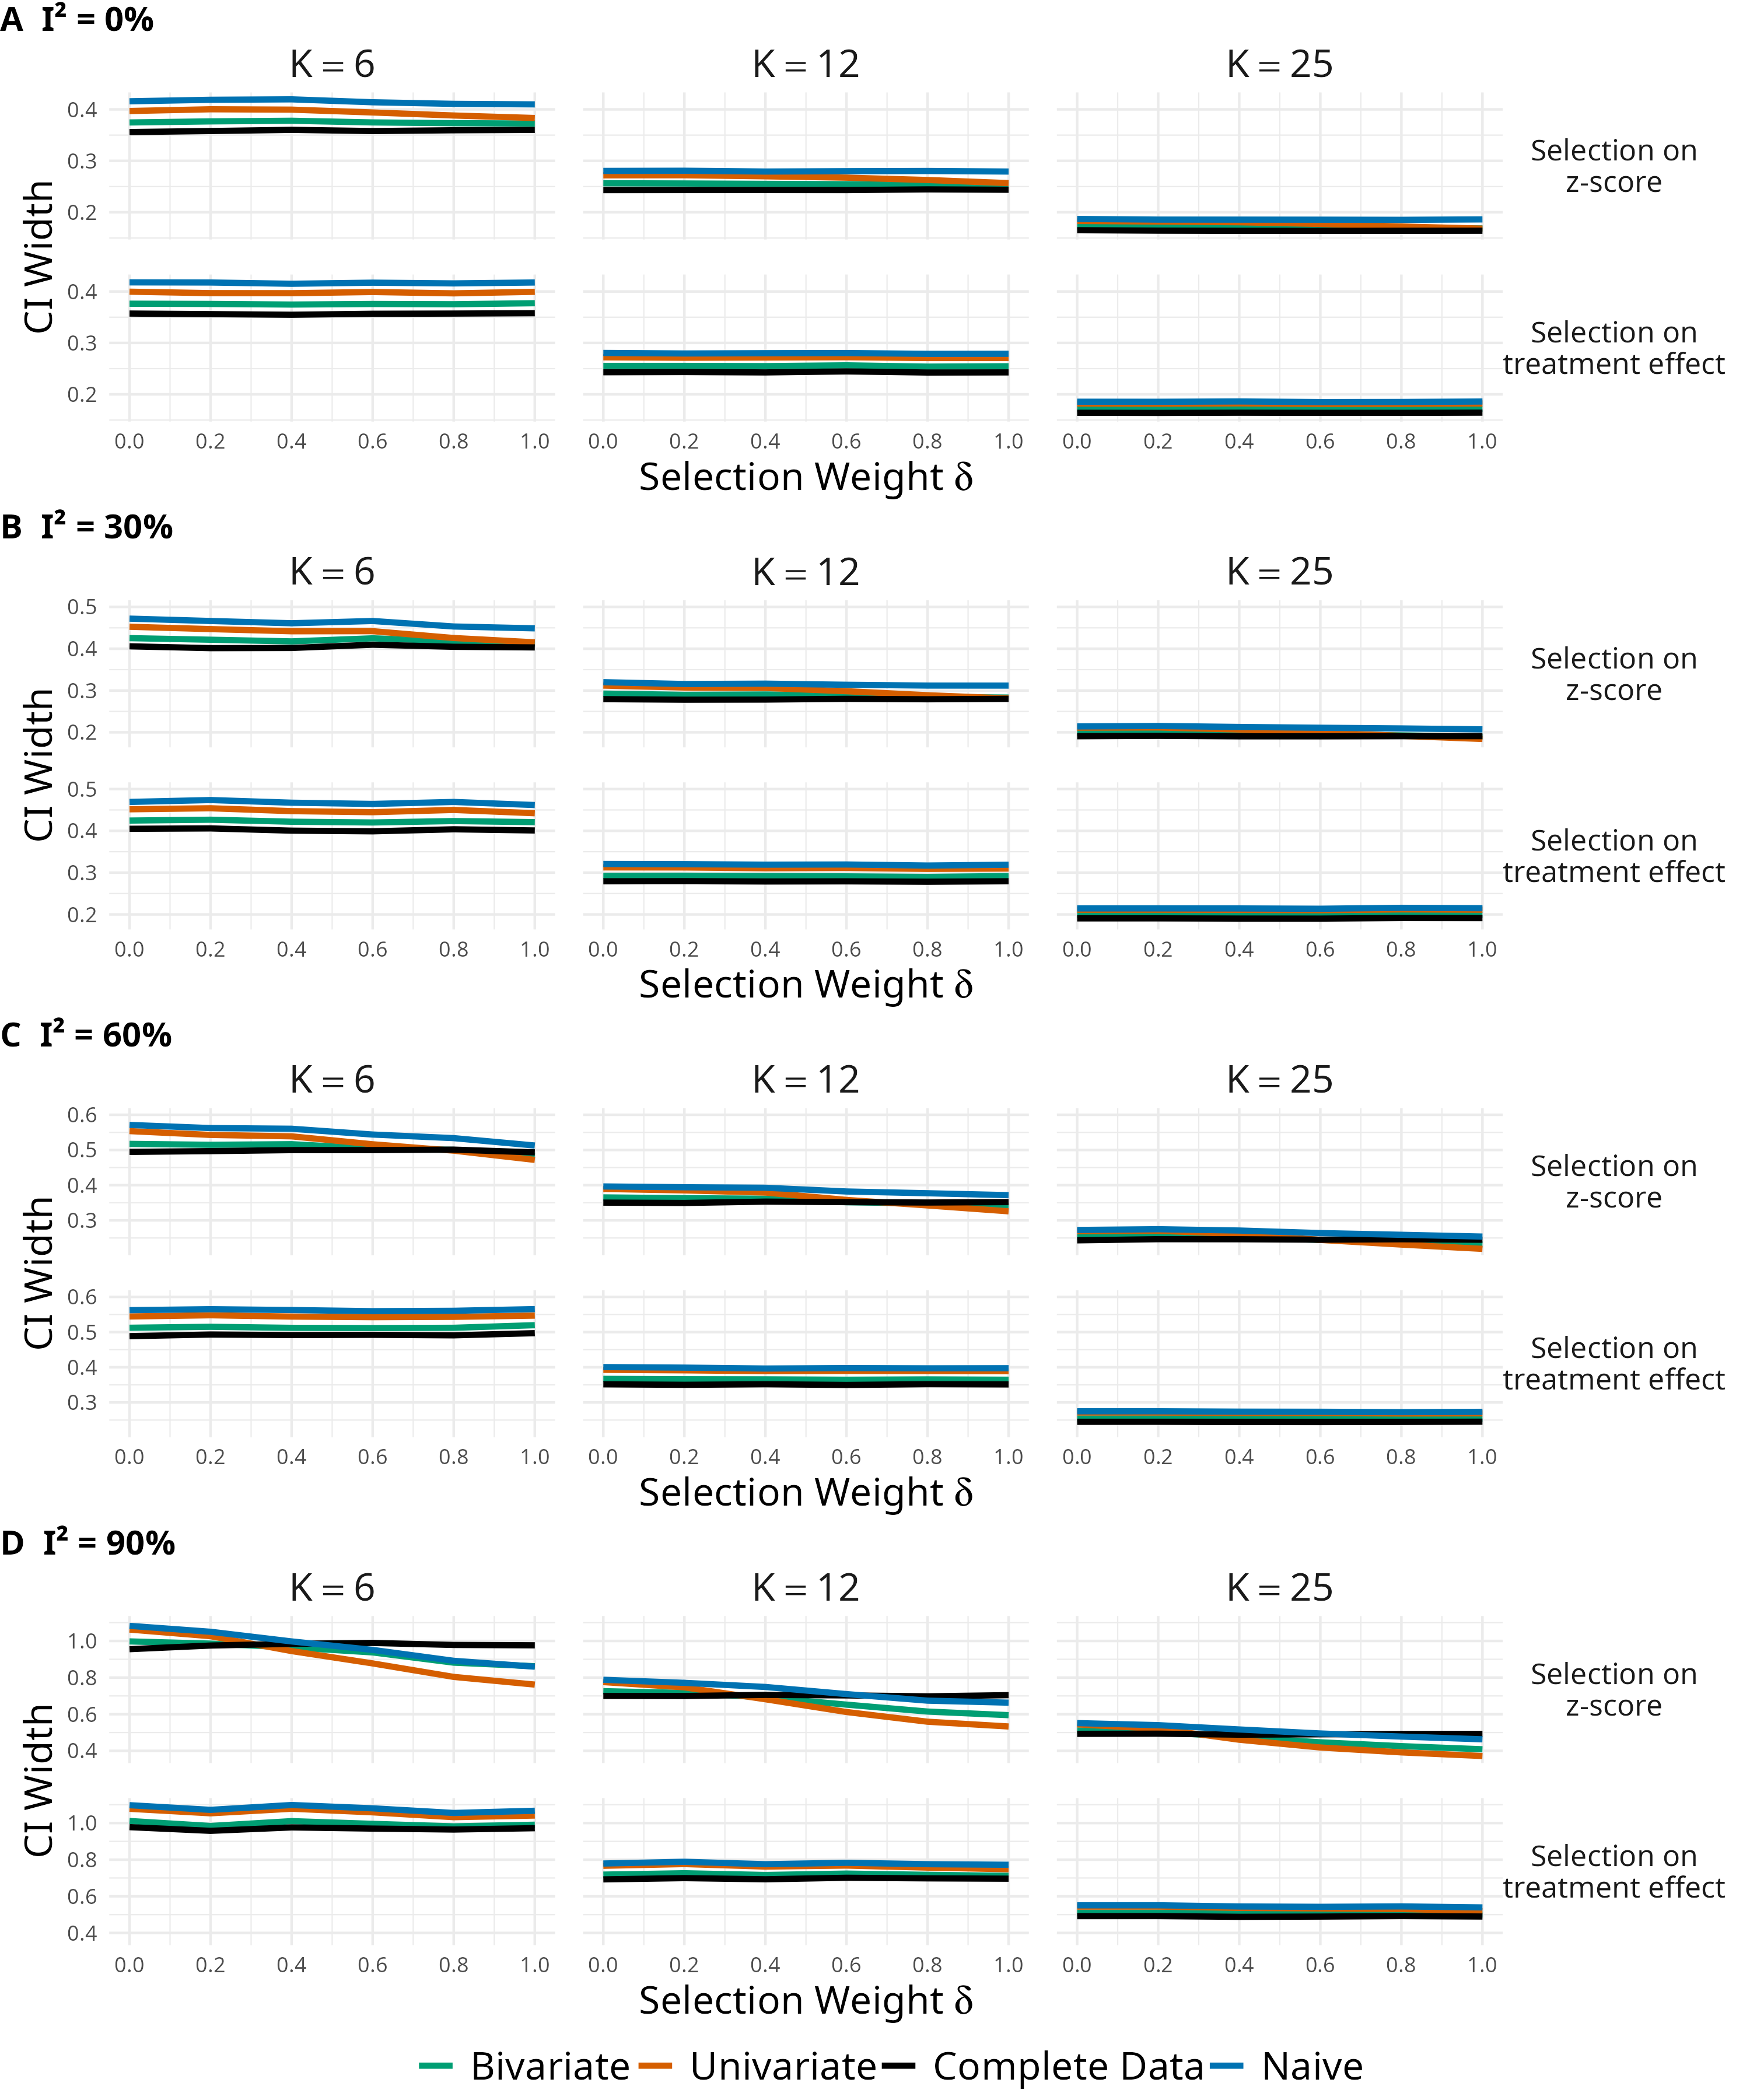
\includegraphics[width = 1\linewidth]{figures/Supp_SimStudy_CIWidth_theta0.png}
\end{figure}

\begin{figure}[!ht]
\centering
\caption{Simulation results for coverage of four MA estimates of the treatment effect for outcome 1 under ORB for $\theta_1 = \theta_2 = 0$, $\rho_B = \rho_W = 0.8$ and $p_1 = 20\%$. Results are shown for varying numbers of studies, heterogeneity levels, selection type, and an increasing selection parameter.}
\label{fig:App_Coverage_theta0}
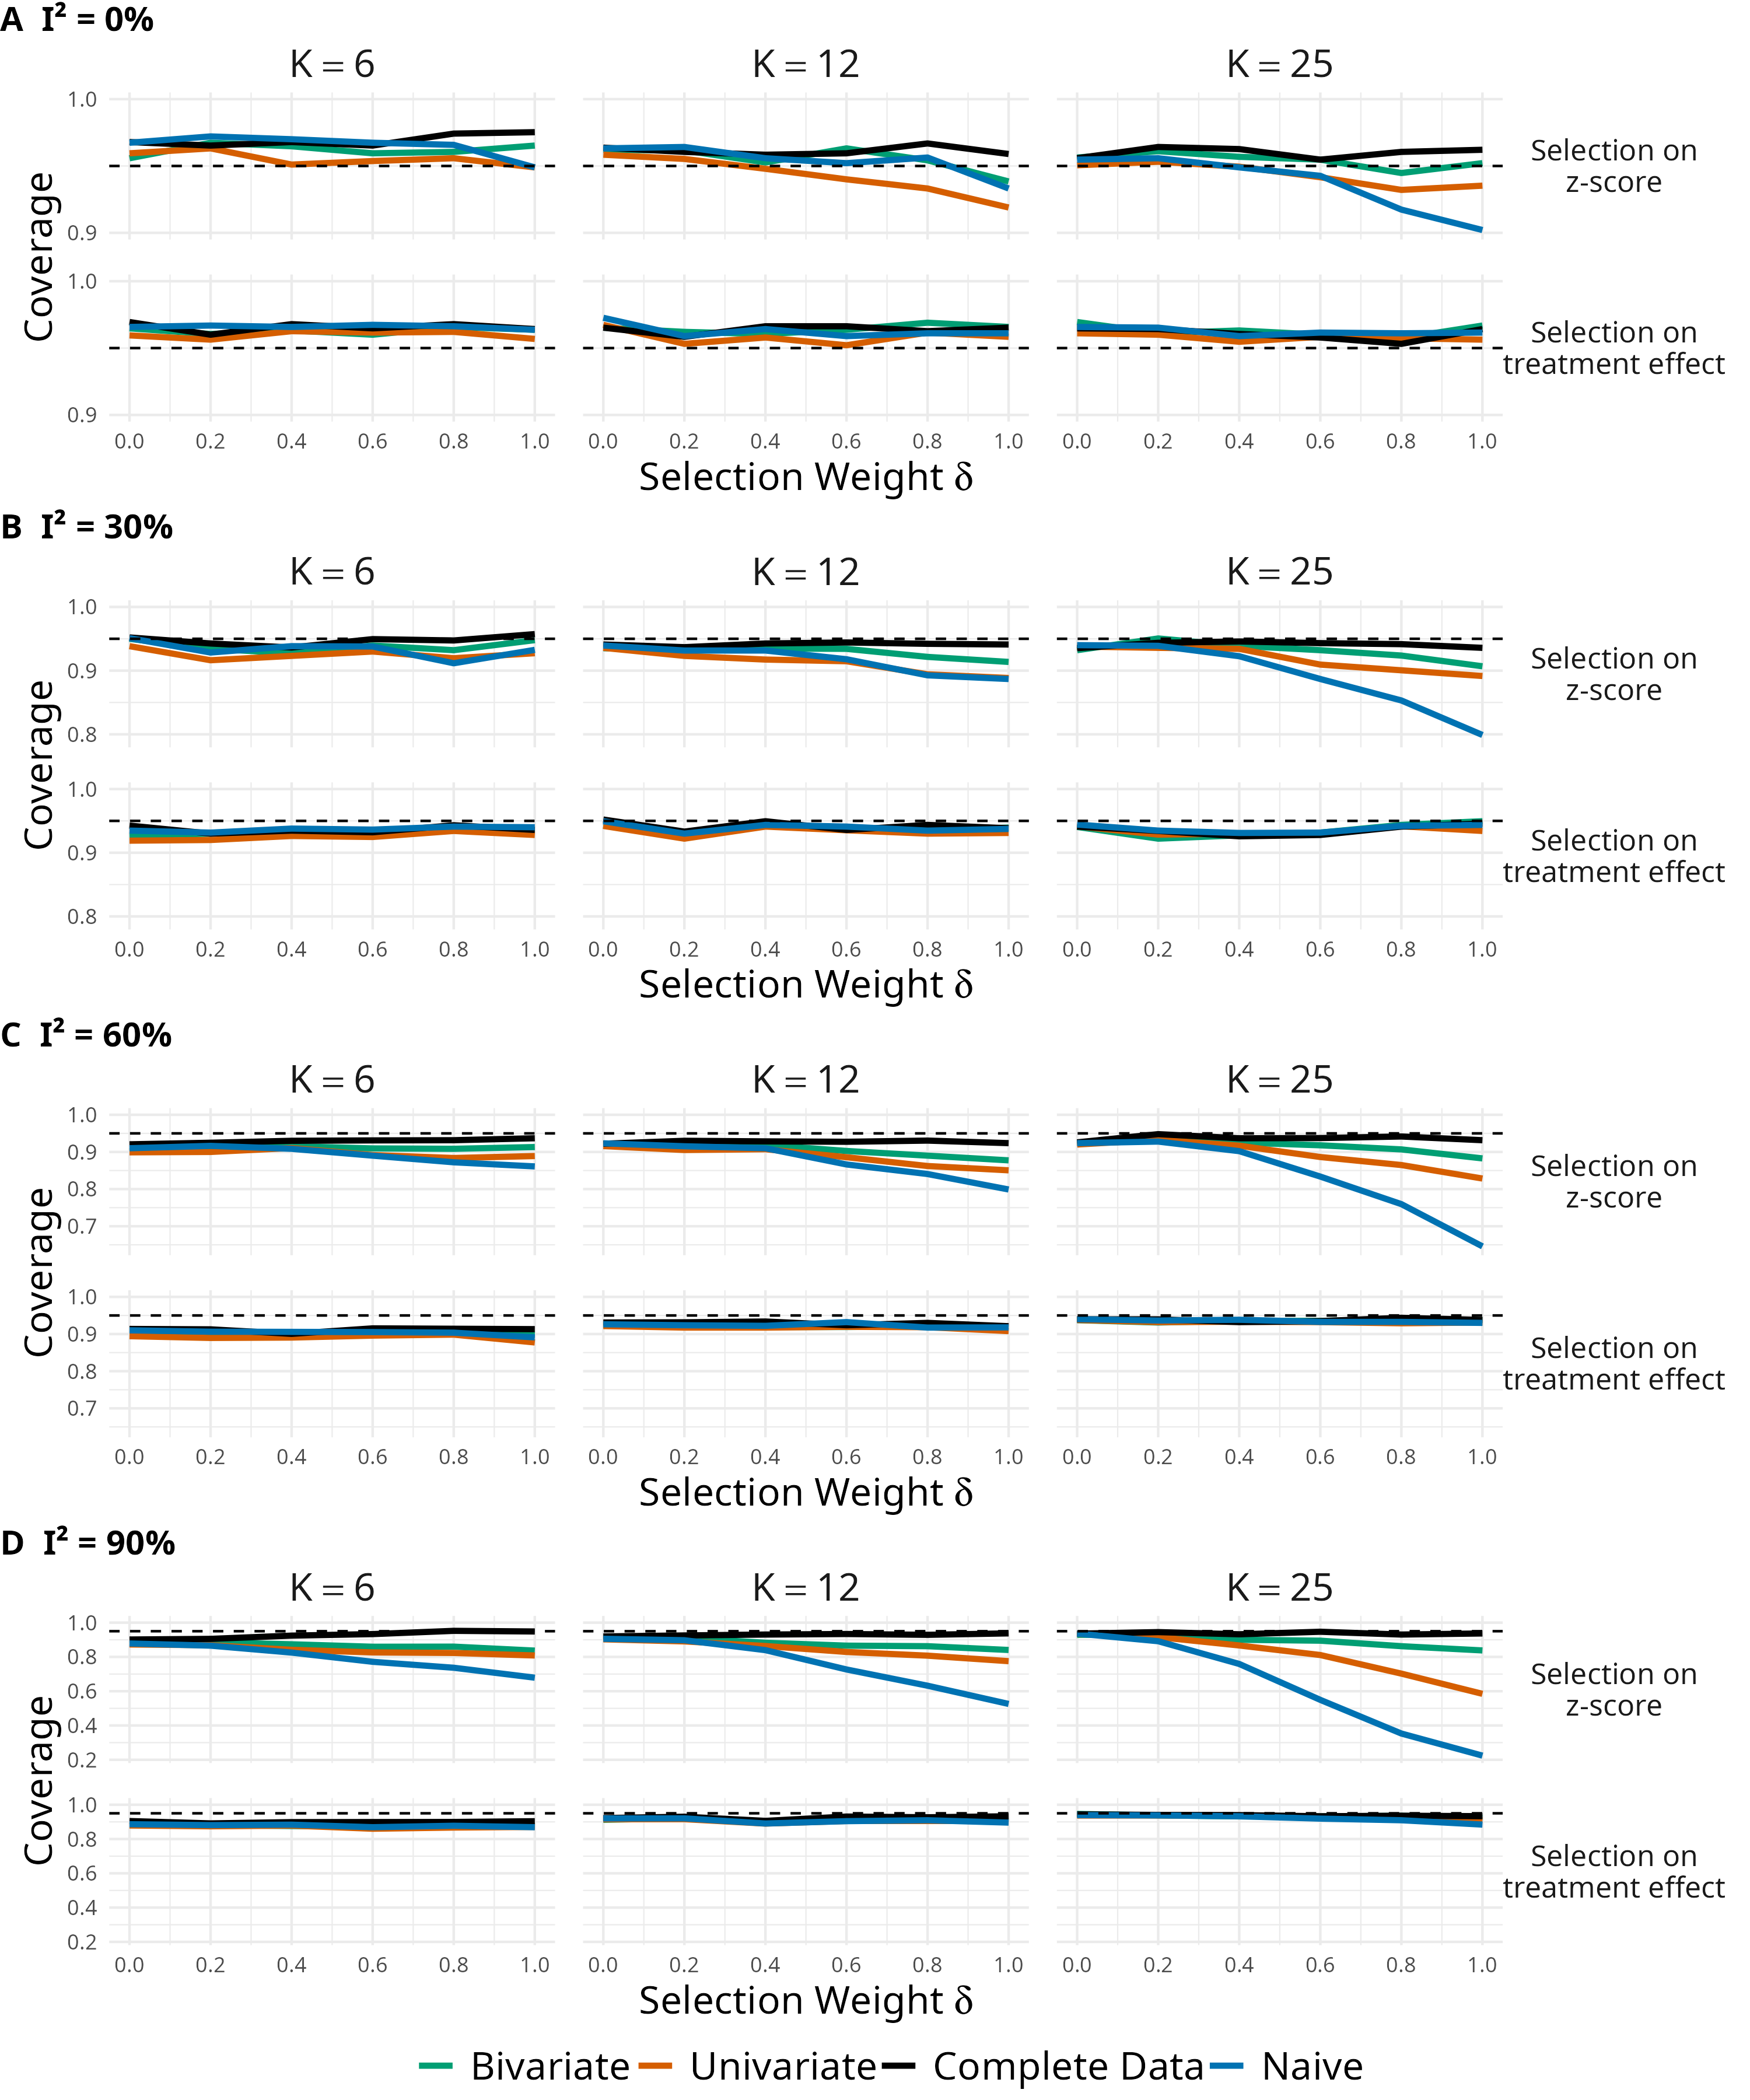
\includegraphics[width = 1\linewidth]{figures/Supp_SimStudy_Coverage_theta0.png}
\end{figure}

\clearpage

\subsection{\mycolor{Additional correlation scenarios}}

\subsubsection{\mycolor{Global correlation model for $\rho_B = \rho_B = 0$}}

\begin{figure}[!ht]
\centering
\caption{Simulation results for bias of four MA estimates of the treatment effect for outcome 1 under ORB for $\theta_1 = \theta_2 = 0.4$, $\rho_B = \rho_W = 0$ and $p_1 = 20\%$. Results are shown for varying numbers of studies, heterogeneity levels, selection type, and an increasing selection parameter.}
\label{fig:App_Bias_rho0}
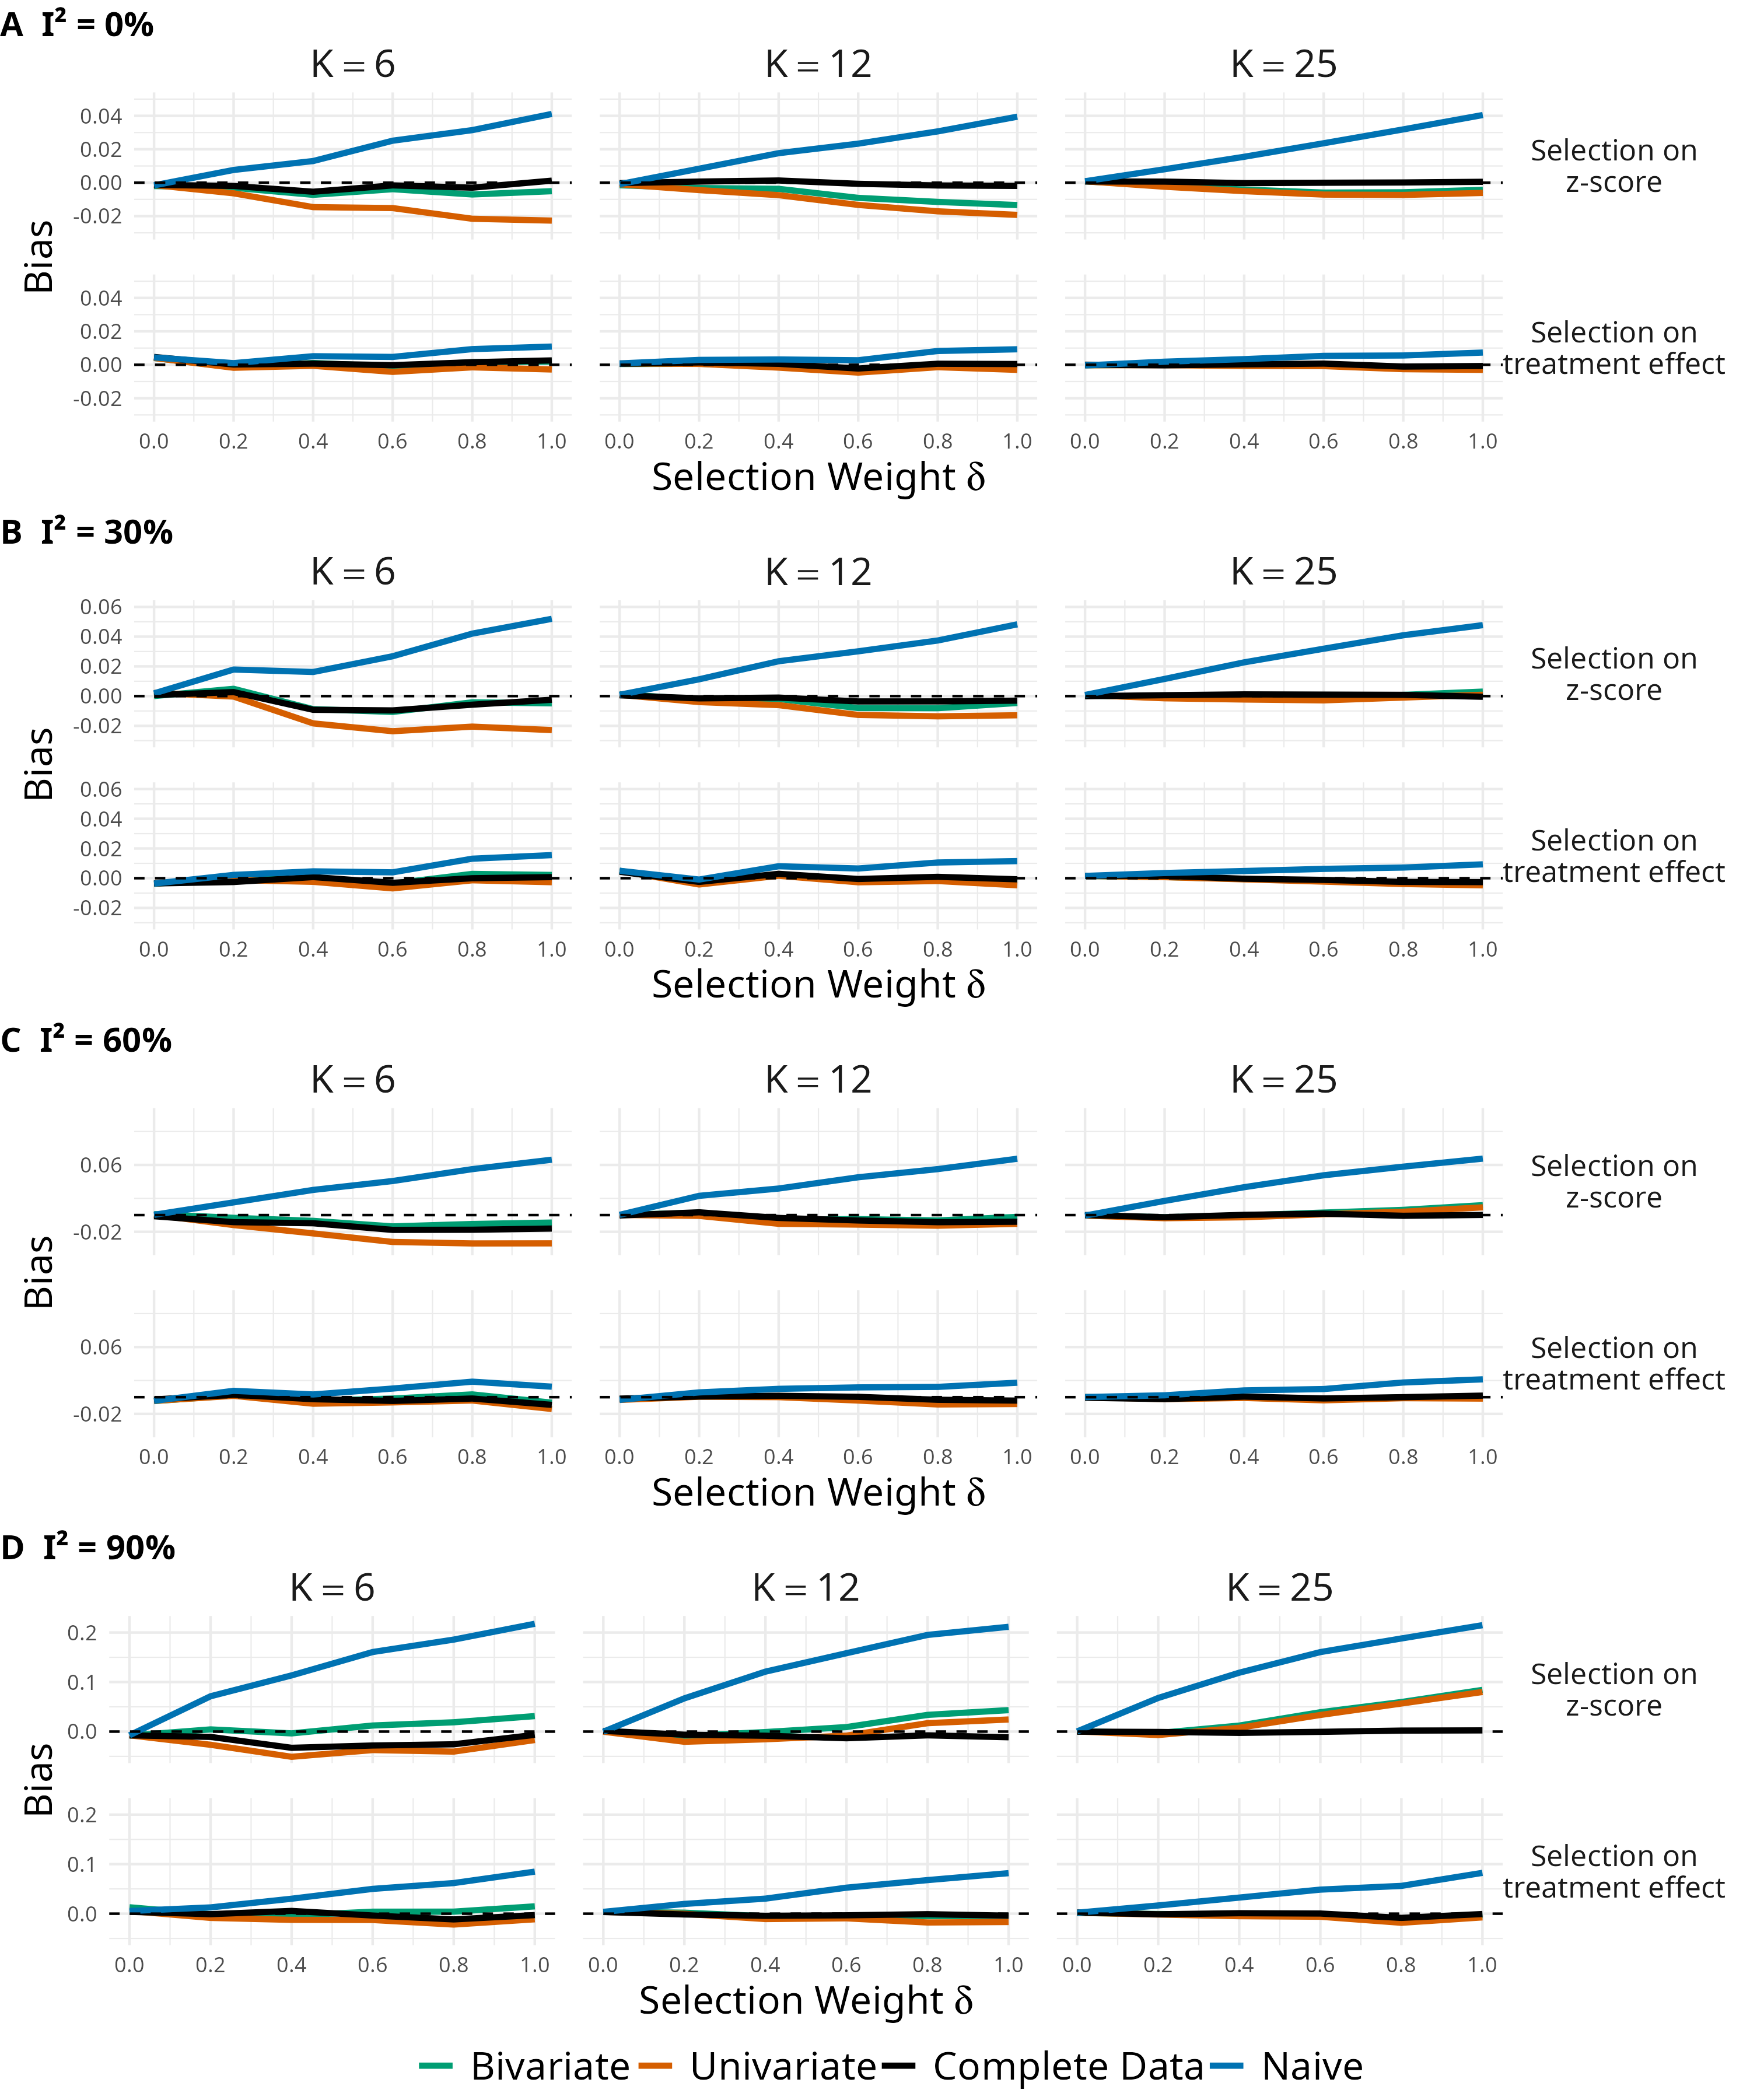
\includegraphics[width = 1\linewidth]{figures/Supp_SimStudy_Bias_rho0.png}
\end{figure}

\begin{figure}[!ht]
\centering
\caption{Simulation results for MSE of four MA estimates of the treatment effect for outcome 1 under ORB for $\theta_1 = \theta_2 = 0.4$, $\rho_B = \rho_W = 0$ and $p_1 = 20\%$. Results are shown for varying numbers of studies, heterogeneity levels, selection type, and an increasing selection parameter.}
\label{fig:App_MSE_rho0}
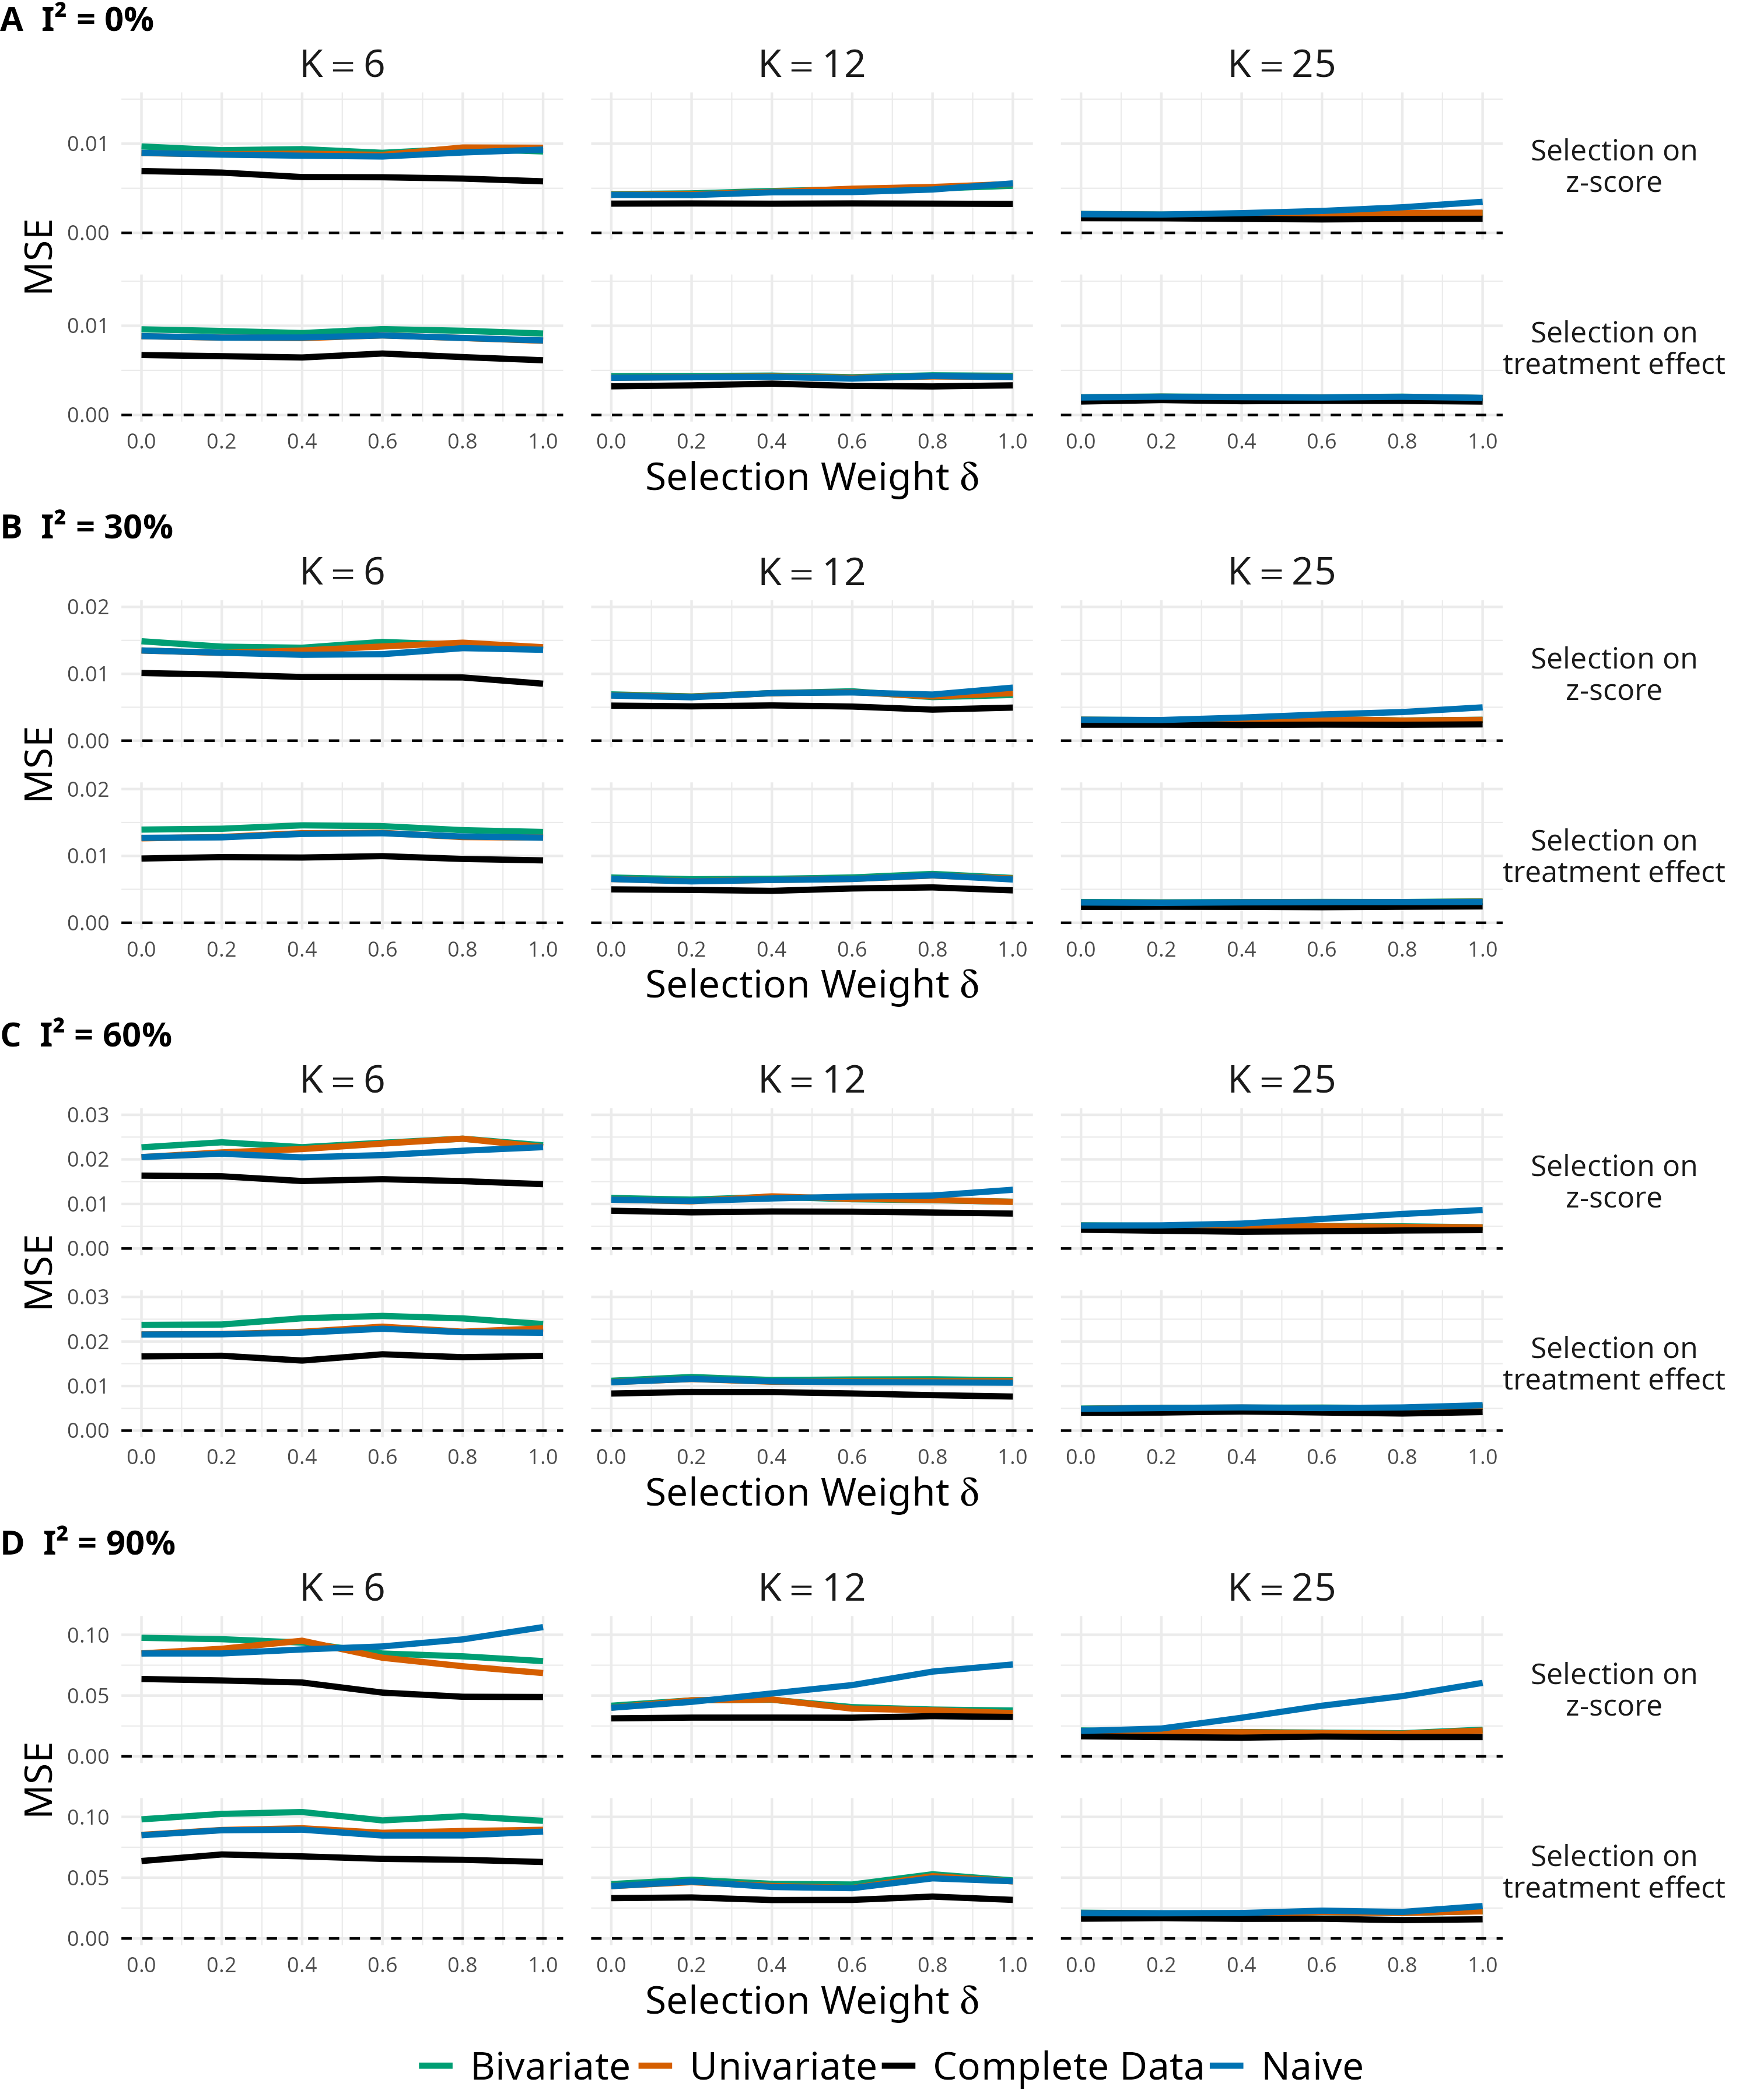
\includegraphics[width = 1\linewidth]{figures/Supp_SimStudy_MSE_rho0.png}
\end{figure}

\begin{figure}[!ht]
\centering
\caption{Simulation results for CI width of four MA estimates of the treatment effect for outcome 1 under ORB for $\theta_1 = \theta_2 = 0.4$, $\rho_B = \rho_W = 0$ and $p_1 = 20\%$. Results are shown for varying numbers of studies, heterogeneity levels, selection type, and an increasing selection parameter.}
\label{fig:App_CIWidth_rho0}
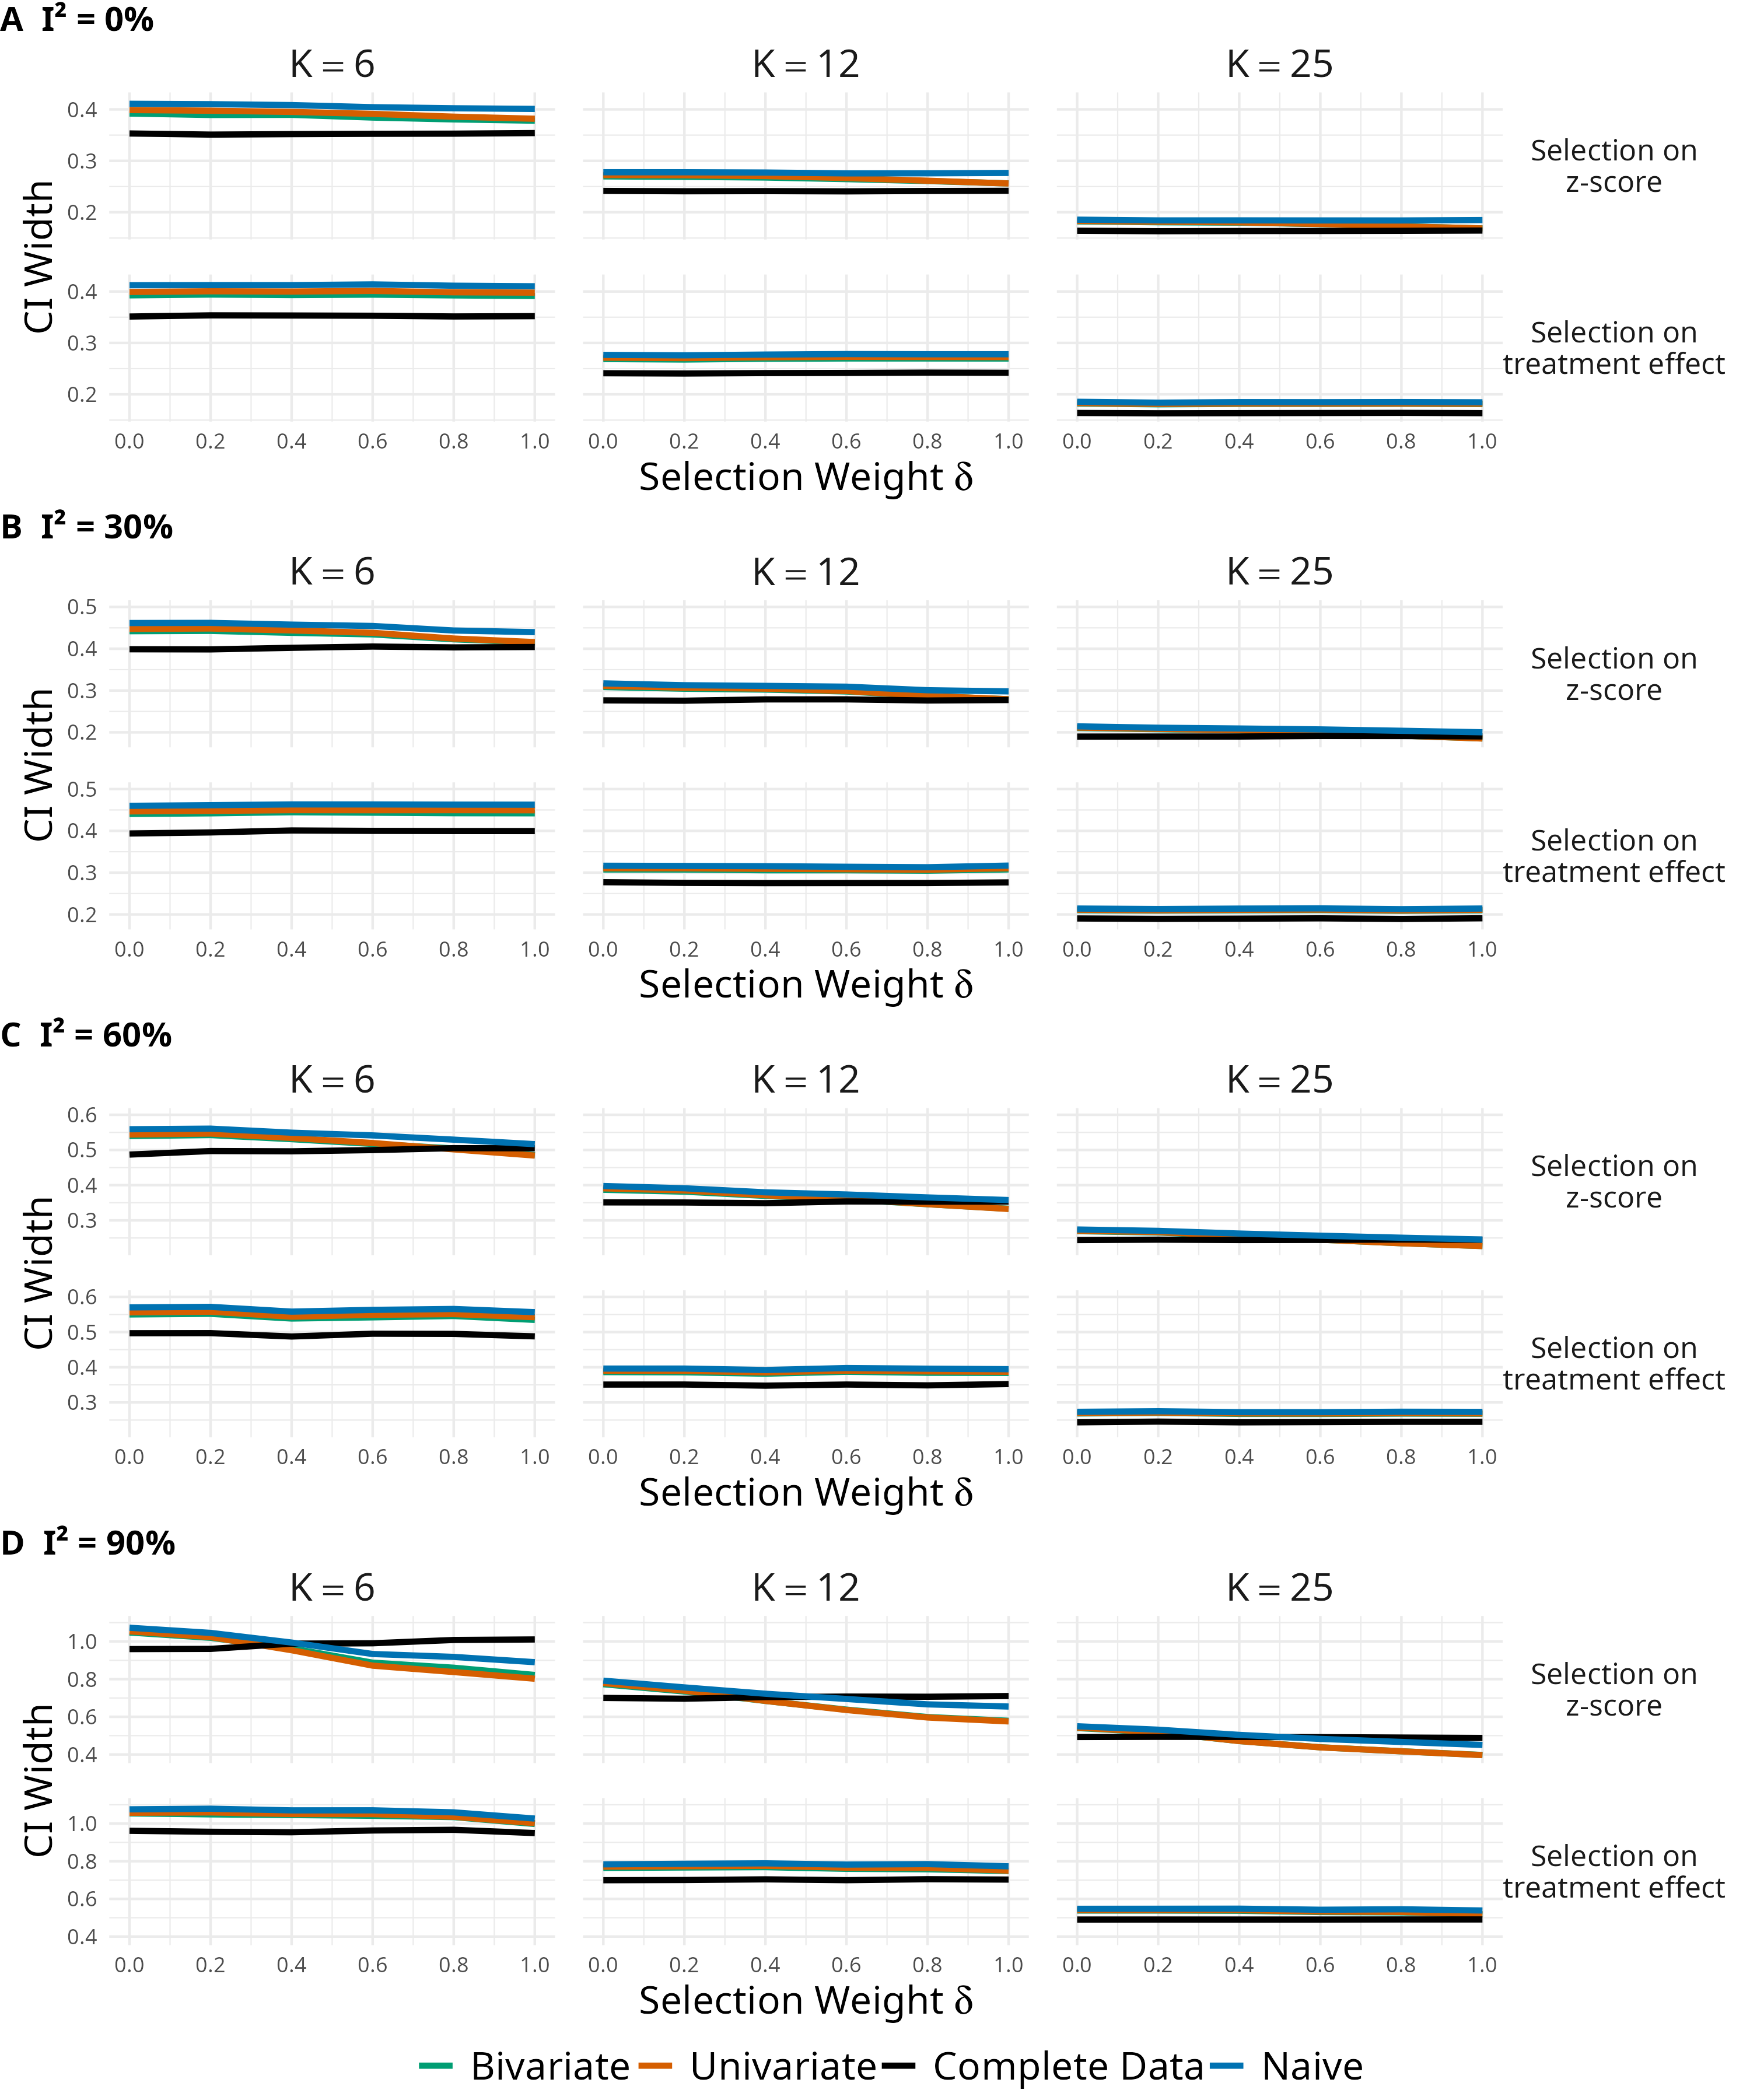
\includegraphics[width = 1\linewidth]{figures/Supp_SimStudy_CIWidth_rho0.png}
\end{figure}

\begin{figure}[!ht]
\centering
\caption{Simulation results for coverage of four MA estimates of the treatment effect for outcome 1 under ORB for $\theta_1 = \theta_2 = 0.4$, $\rho_B = \rho_W = 0$ and $p_1 = 20\%$. Results are shown for varying numbers of studies, heterogeneity levels, selection type, and an increasing selection parameter.}
\label{fig:App_Coverage_rho0}
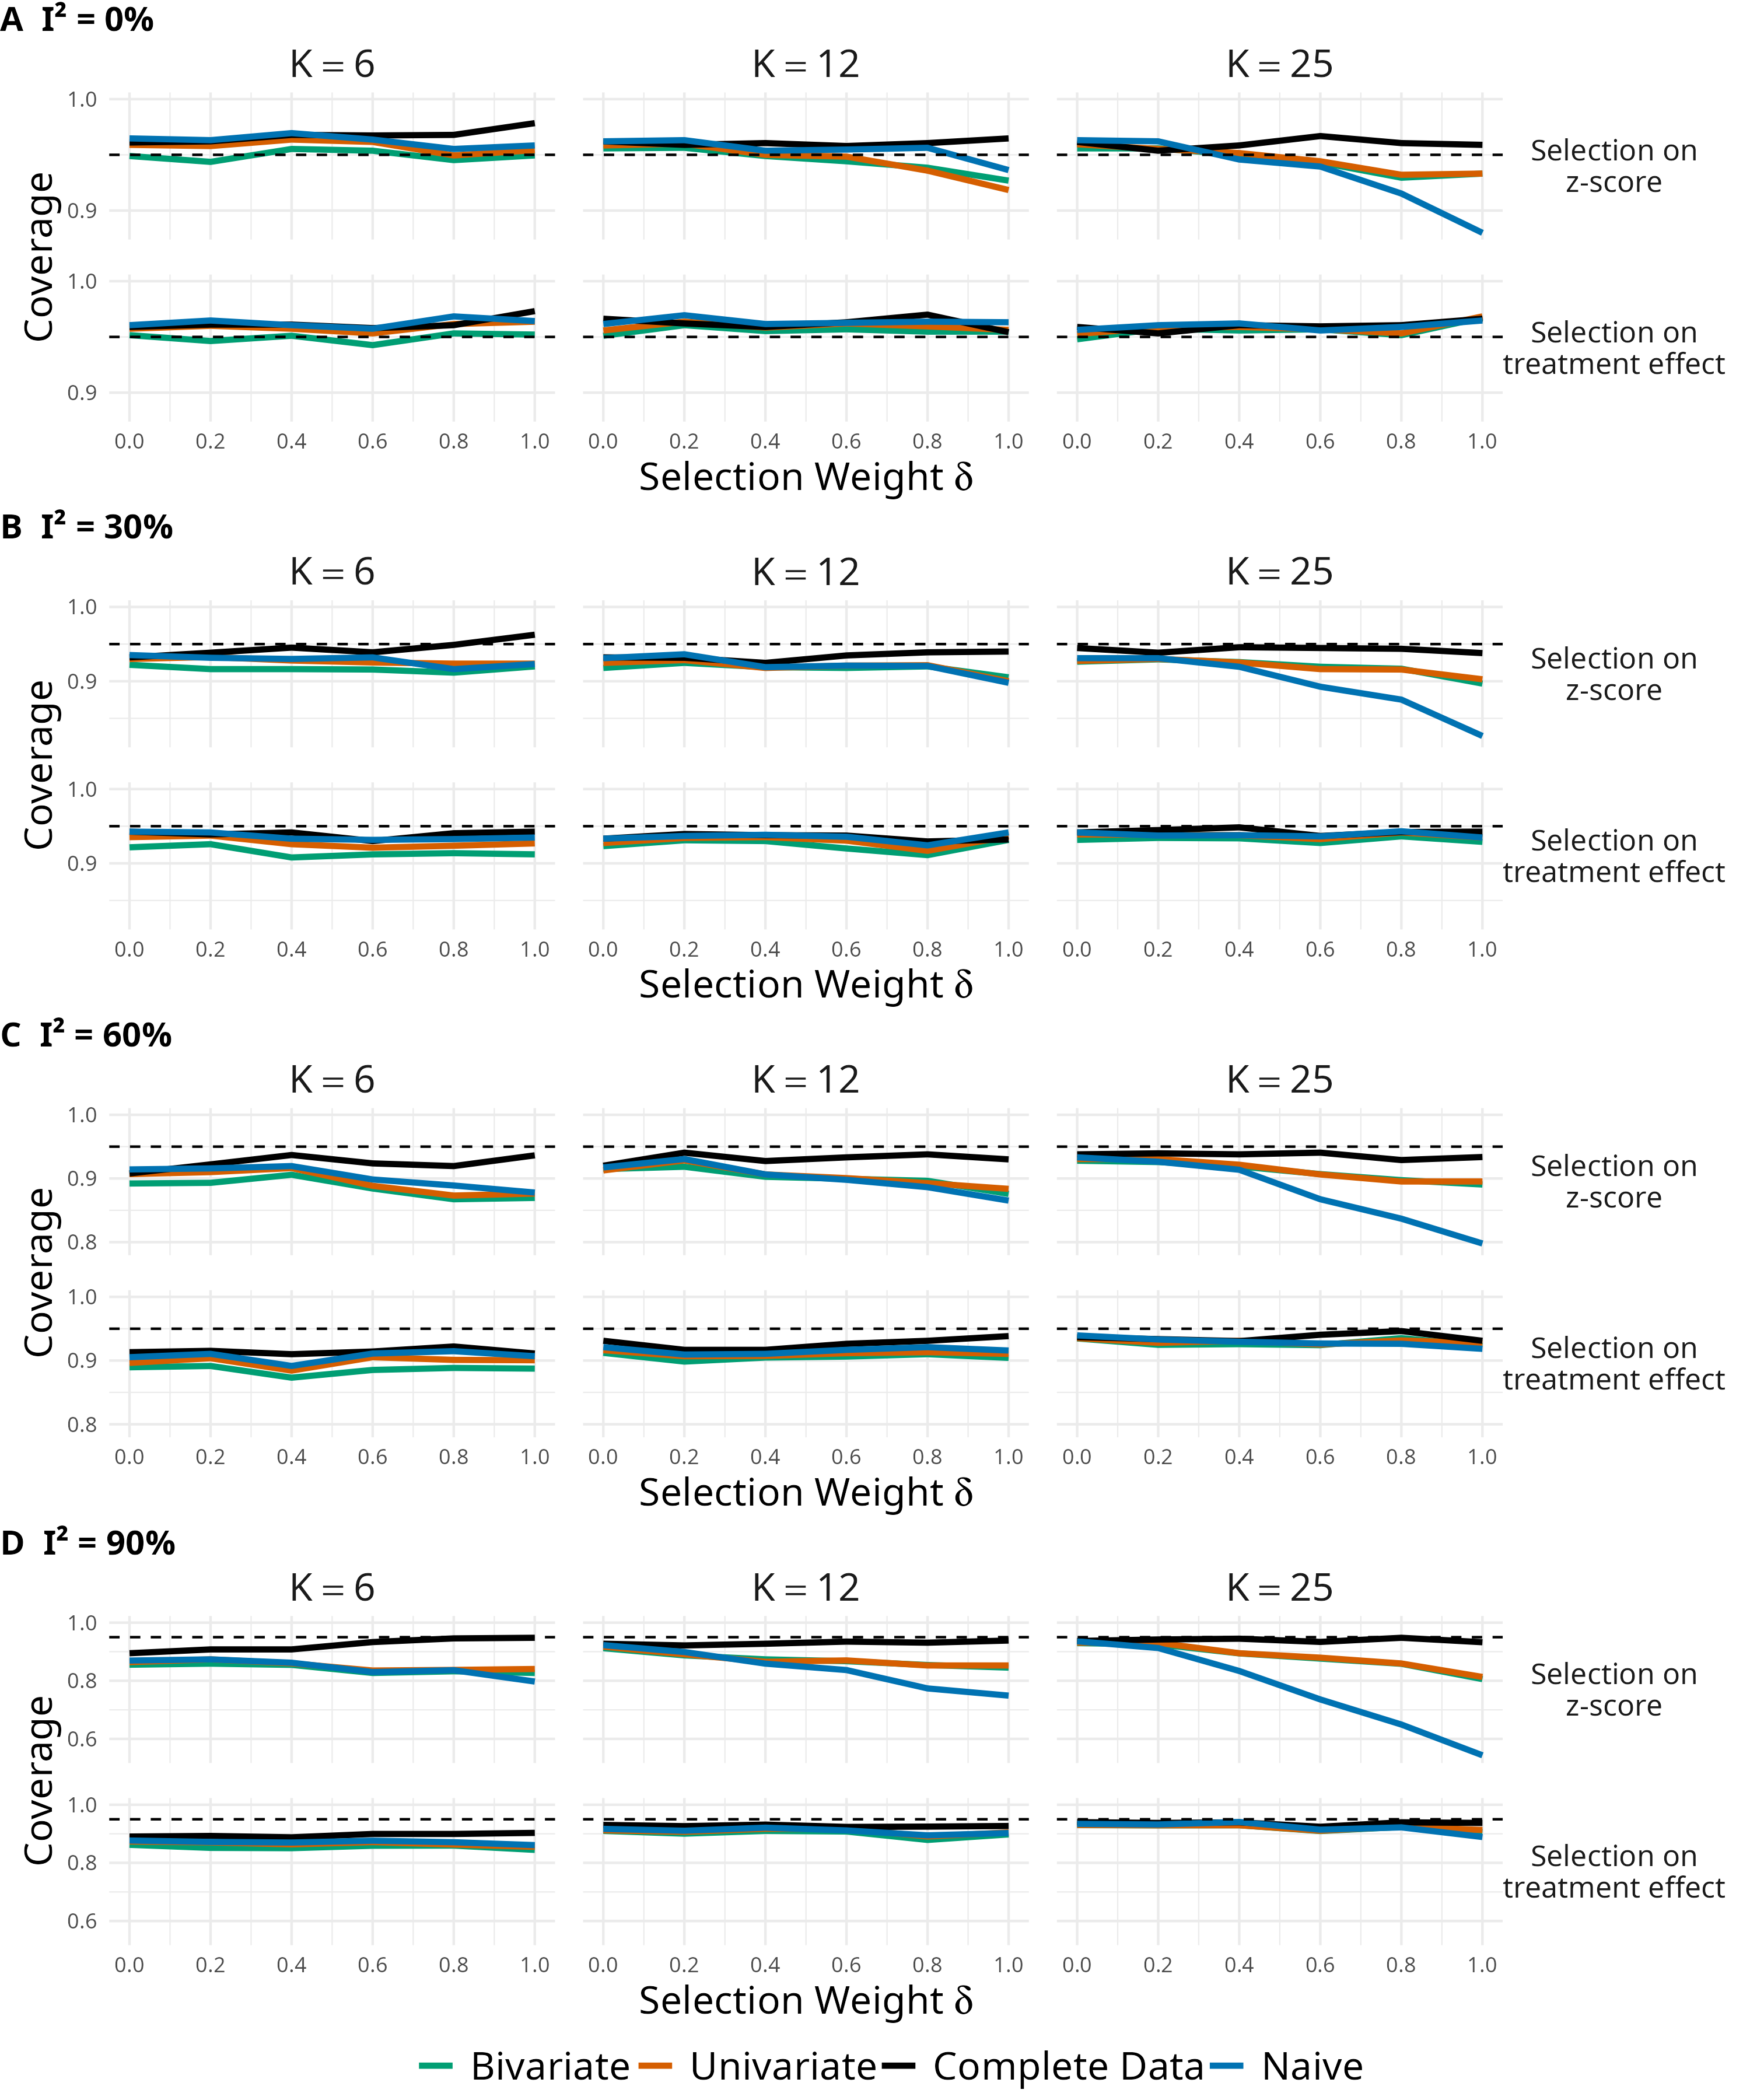
\includegraphics[width = 1\linewidth]{figures/Supp_SimStudy_Coverage_rho0.png}
\end{figure}

\clearpage


\subsubsection{\mycolor{Unequal correlation: $\rho_B = 0.8$, $\rho_W = 0$}}

\begin{figure}[!ht]
\centering
\caption{Simulation results for bias of four MA estimates of the treatment effect for outcome 1 under ORB for $\theta_1 = \theta_2 = 0.4$, $\rho_B = 0.8$, $\rho_W = 0$ and $p_1 = 20\%$. Results are shown for varying numbers of studies, heterogeneity levels, selection type, and an increasing selection parameter.}
\label{fig:App_Bias_rhoW0}
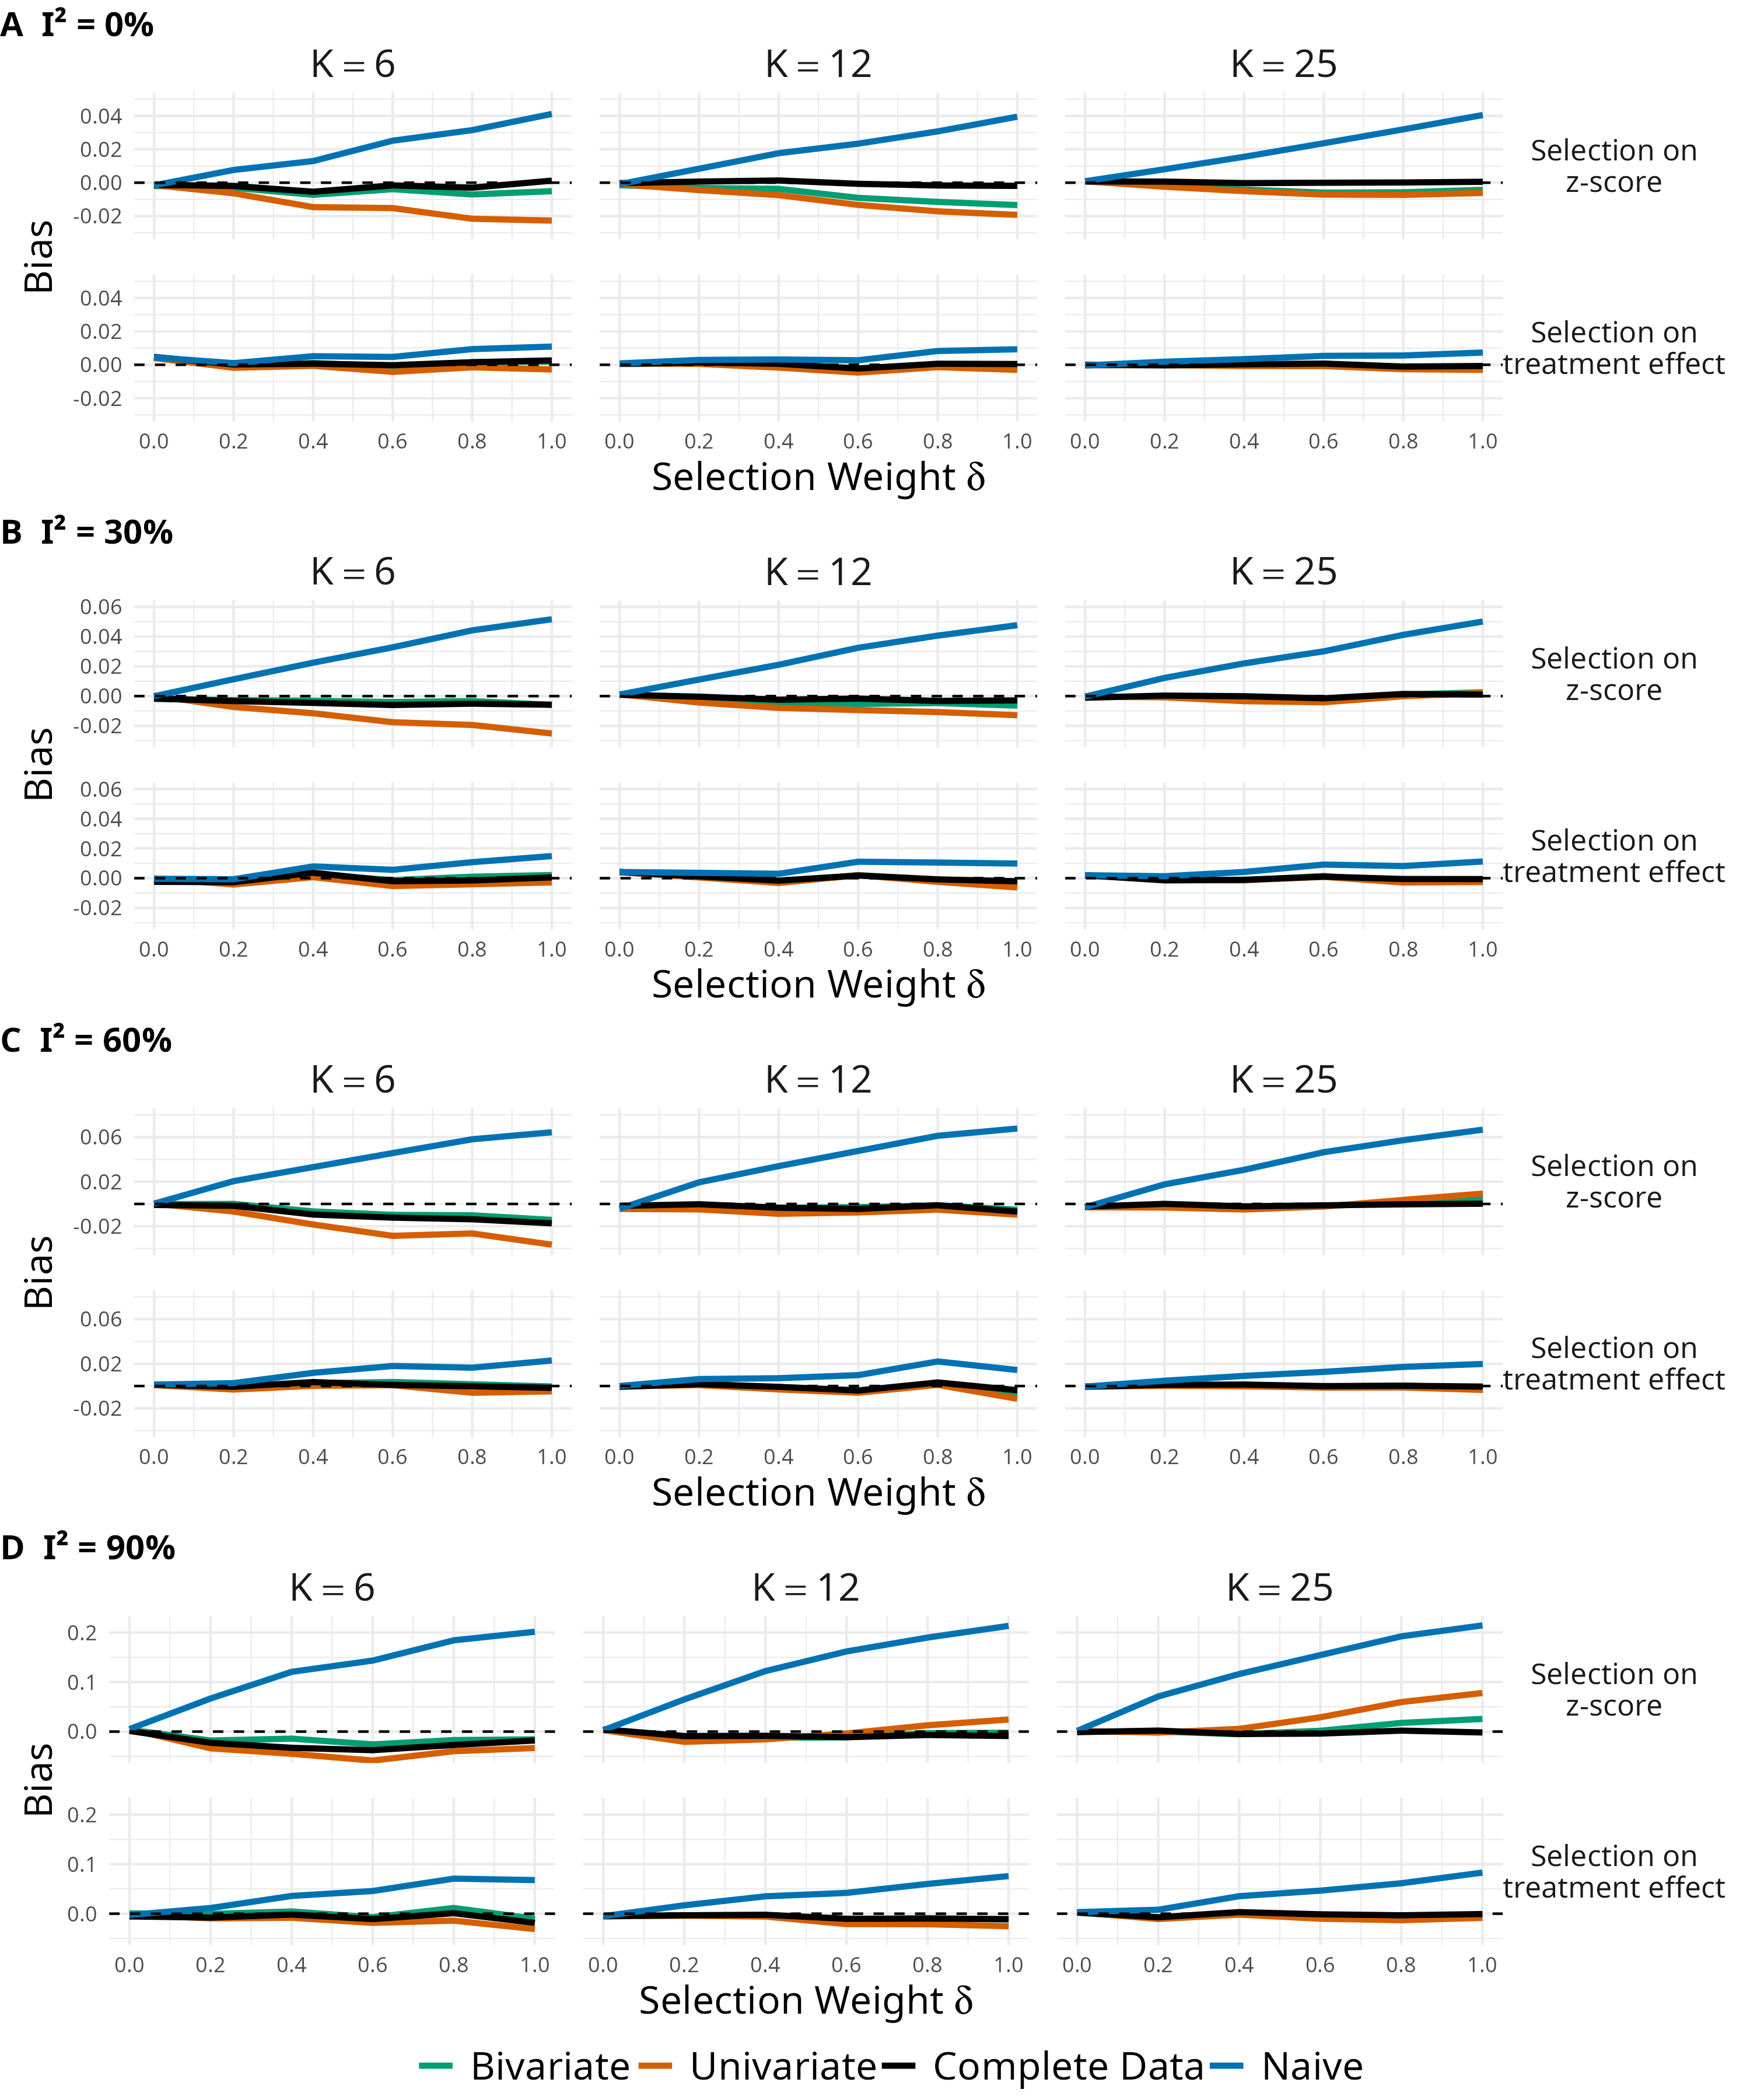
\includegraphics[width = 1\linewidth]{figures/Supp_SimStudy_Bias_rhoW0.png}
\end{figure}

\begin{figure}[!ht]
\centering
\caption{Simulation results for MSE of four MA estimates of the treatment effect for outcome 1 under ORB for $\theta_1 = \theta_2 = 0.4$, $\rho_B = 0.8$, $\rho_W = 0$ and $p_1 = 20\%$. Results are shown for varying numbers of studies, heterogeneity levels, selection type, and an increasing selection parameter.}
\label{fig:App_MSE_rhoW0}
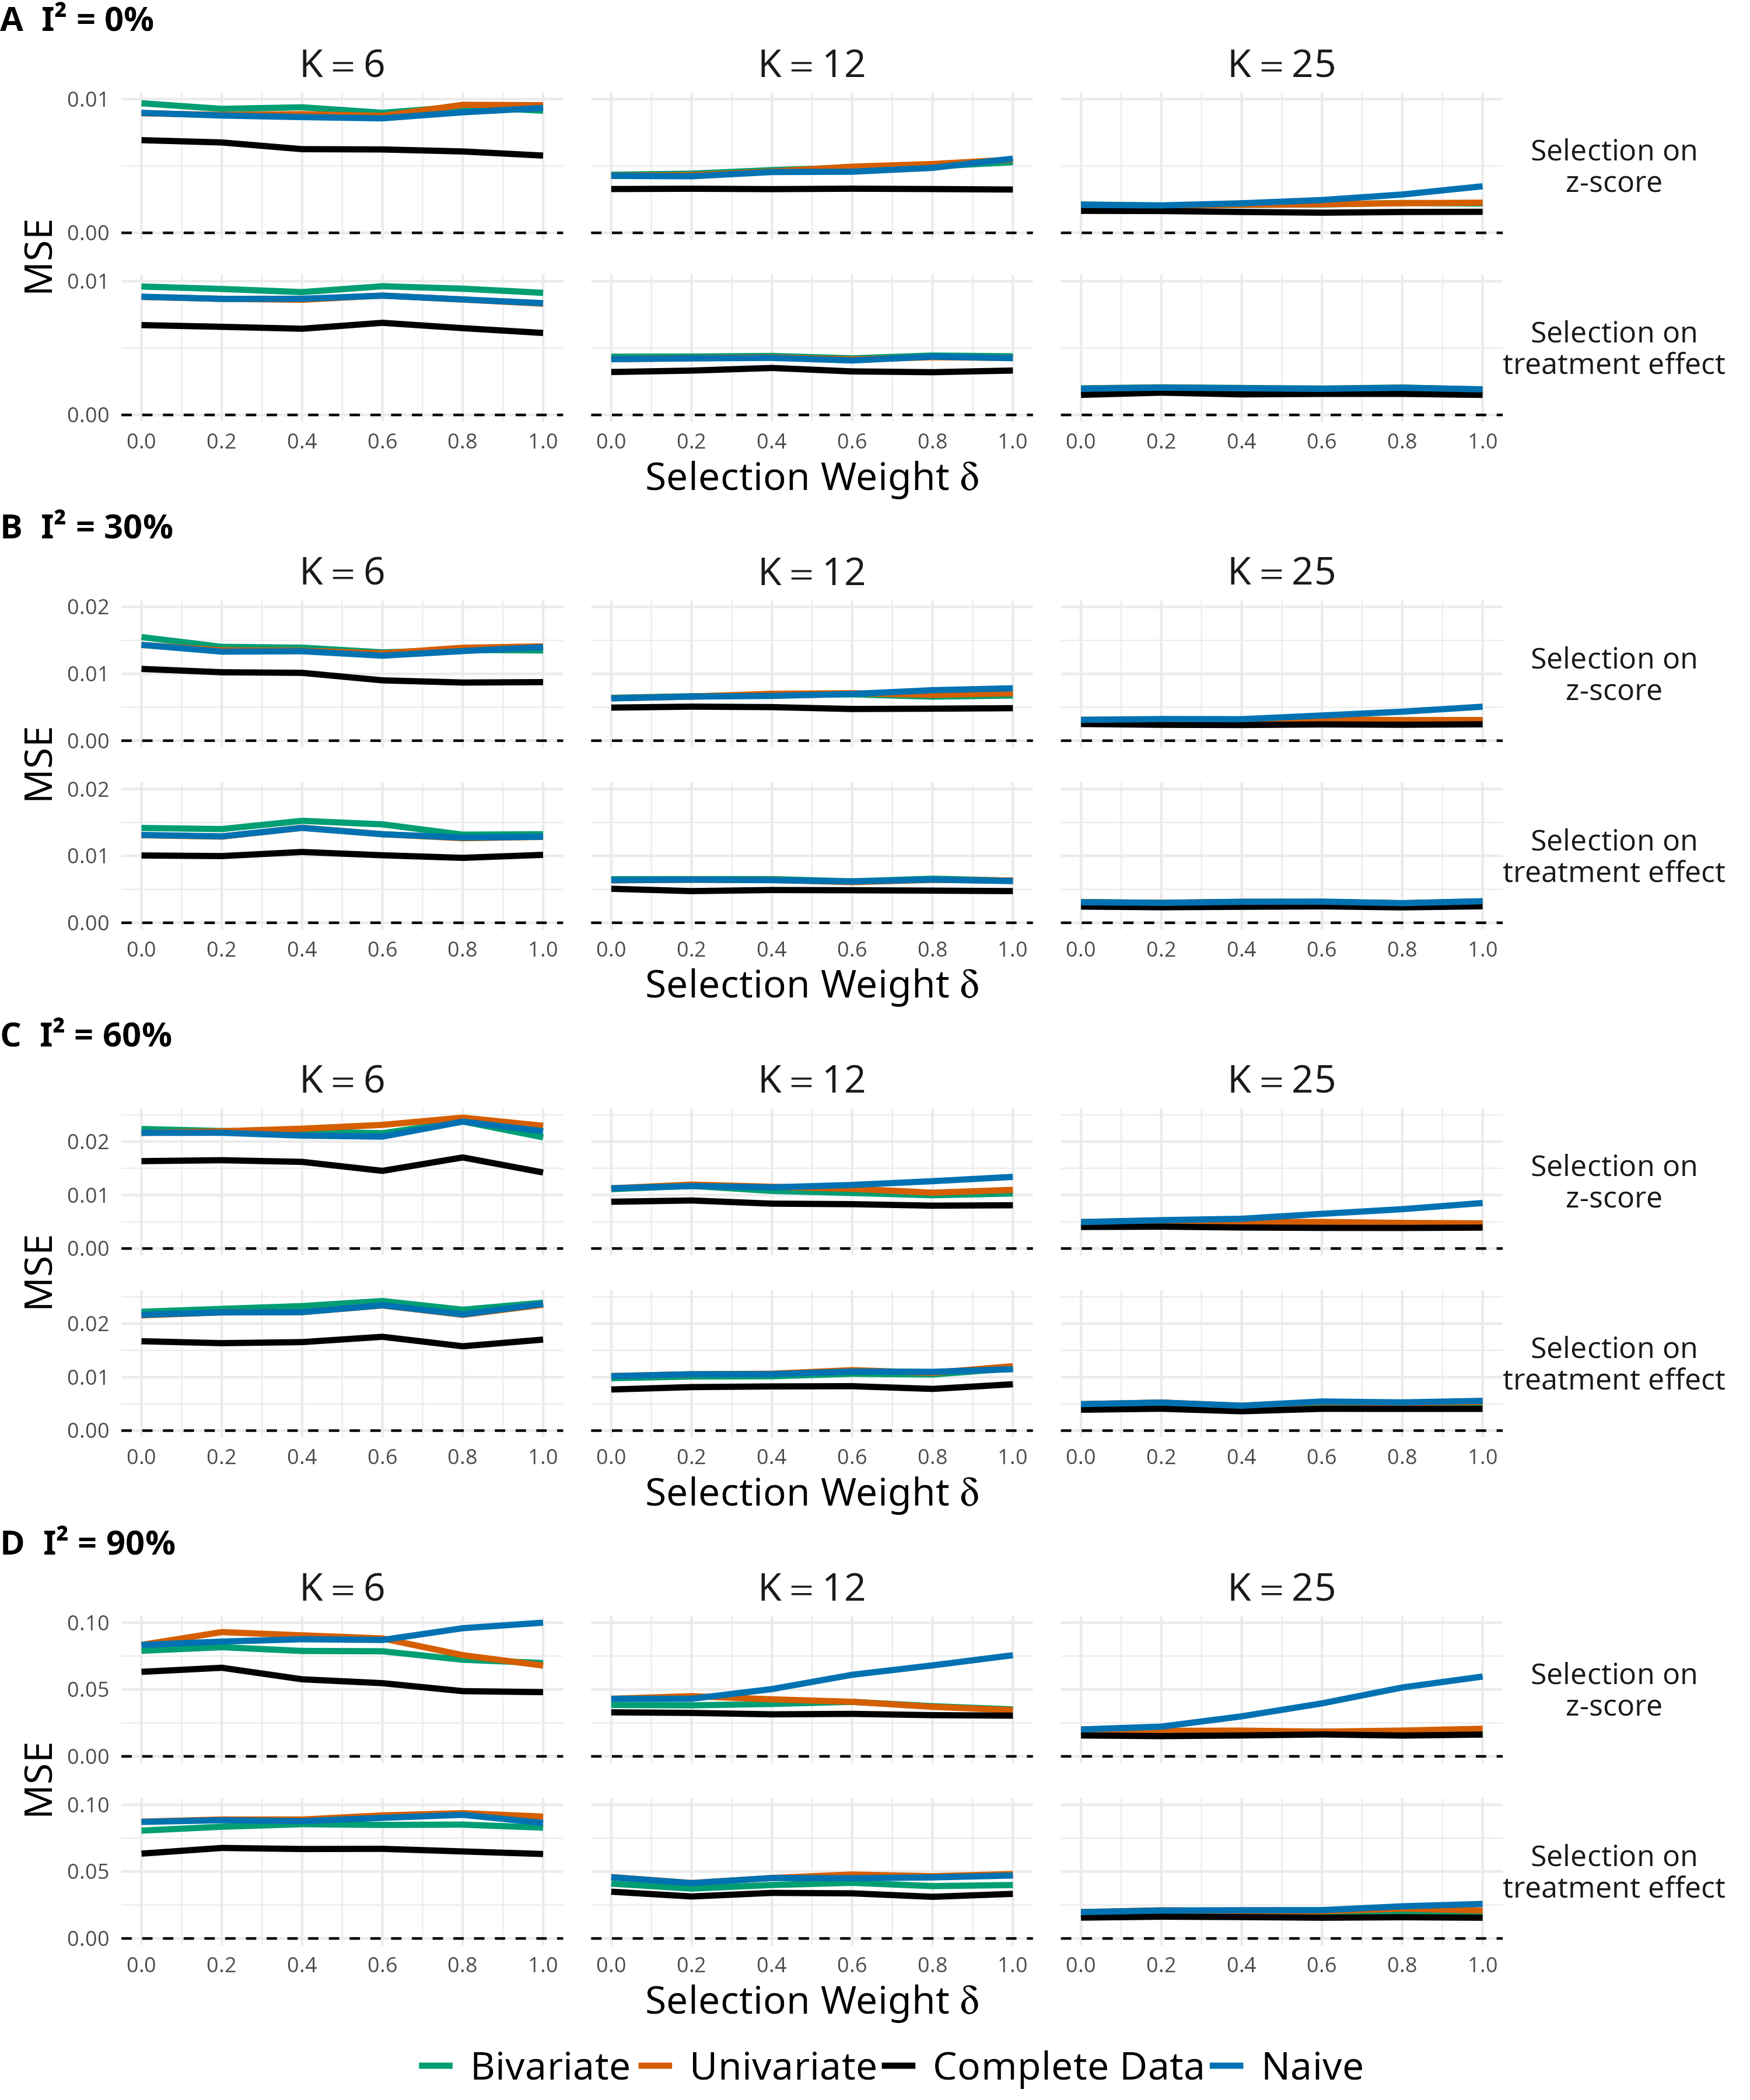
\includegraphics[width = 1\linewidth]{figures/Supp_SimStudy_MSE_rhoW0.png}
\end{figure}

\begin{figure}[!ht]
\centering
\caption{Simulation results for CI width of four MA estimates of the treatment effect for outcome 1 under ORB for $\theta_1 = \theta_2 = 0.4$, $\rho_B = 0.8$, $\rho_W = 0$ and $p_1 = 20\%$. Results are shown for varying numbers of studies, heterogeneity levels, selection type, and an increasing selection parameter.}
\label{fig:App_CIWidth_rhoW0}
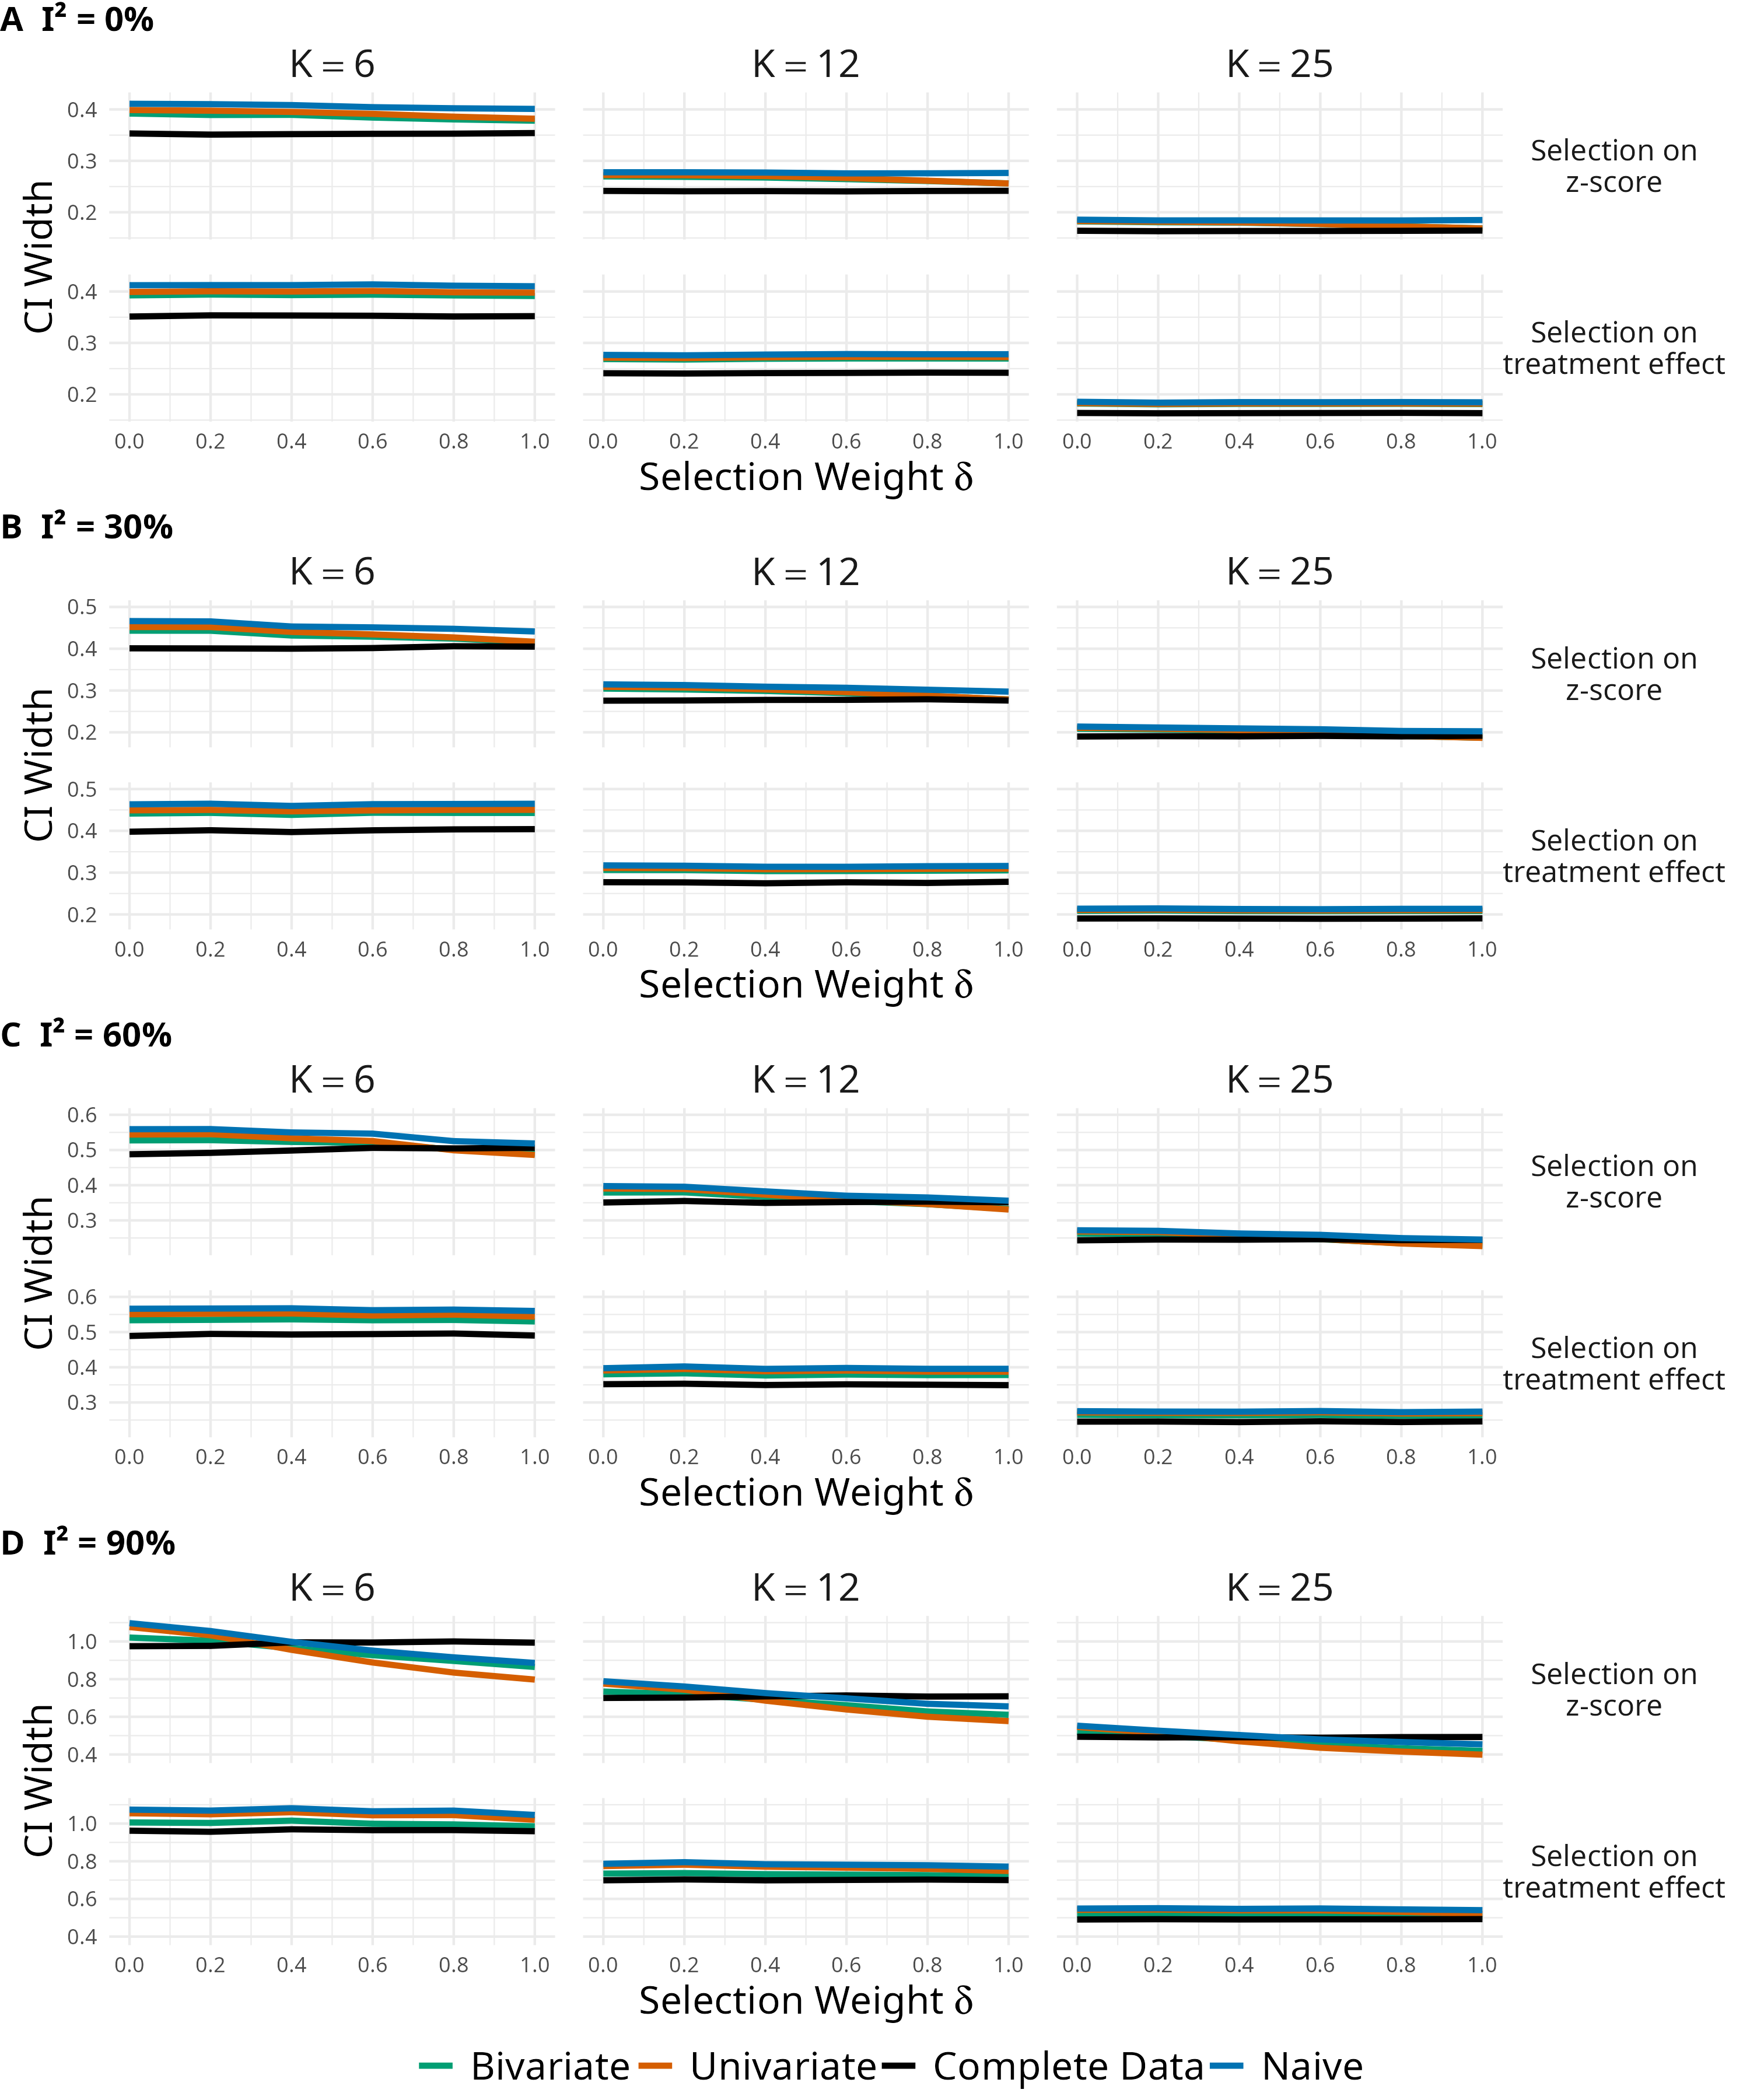
\includegraphics[width = 1\linewidth]{figures/Supp_SimStudy_CIWidth_rhoW0.png}
\end{figure}

\begin{figure}[!ht]
\centering
\caption{Simulation results for coverage of four MA estimates of the treatment effect for outcome 1 under ORB for $\theta_1 = \theta_2 = 0.4$, $\rho_B = 0.8$, $\rho_W = 0$ and $p_1 = 20\%$. Results are shown for varying numbers of studies, heterogeneity levels, selection type, and an increasing selection parameter.}
\label{fig:App_Coverage_rhoW0}
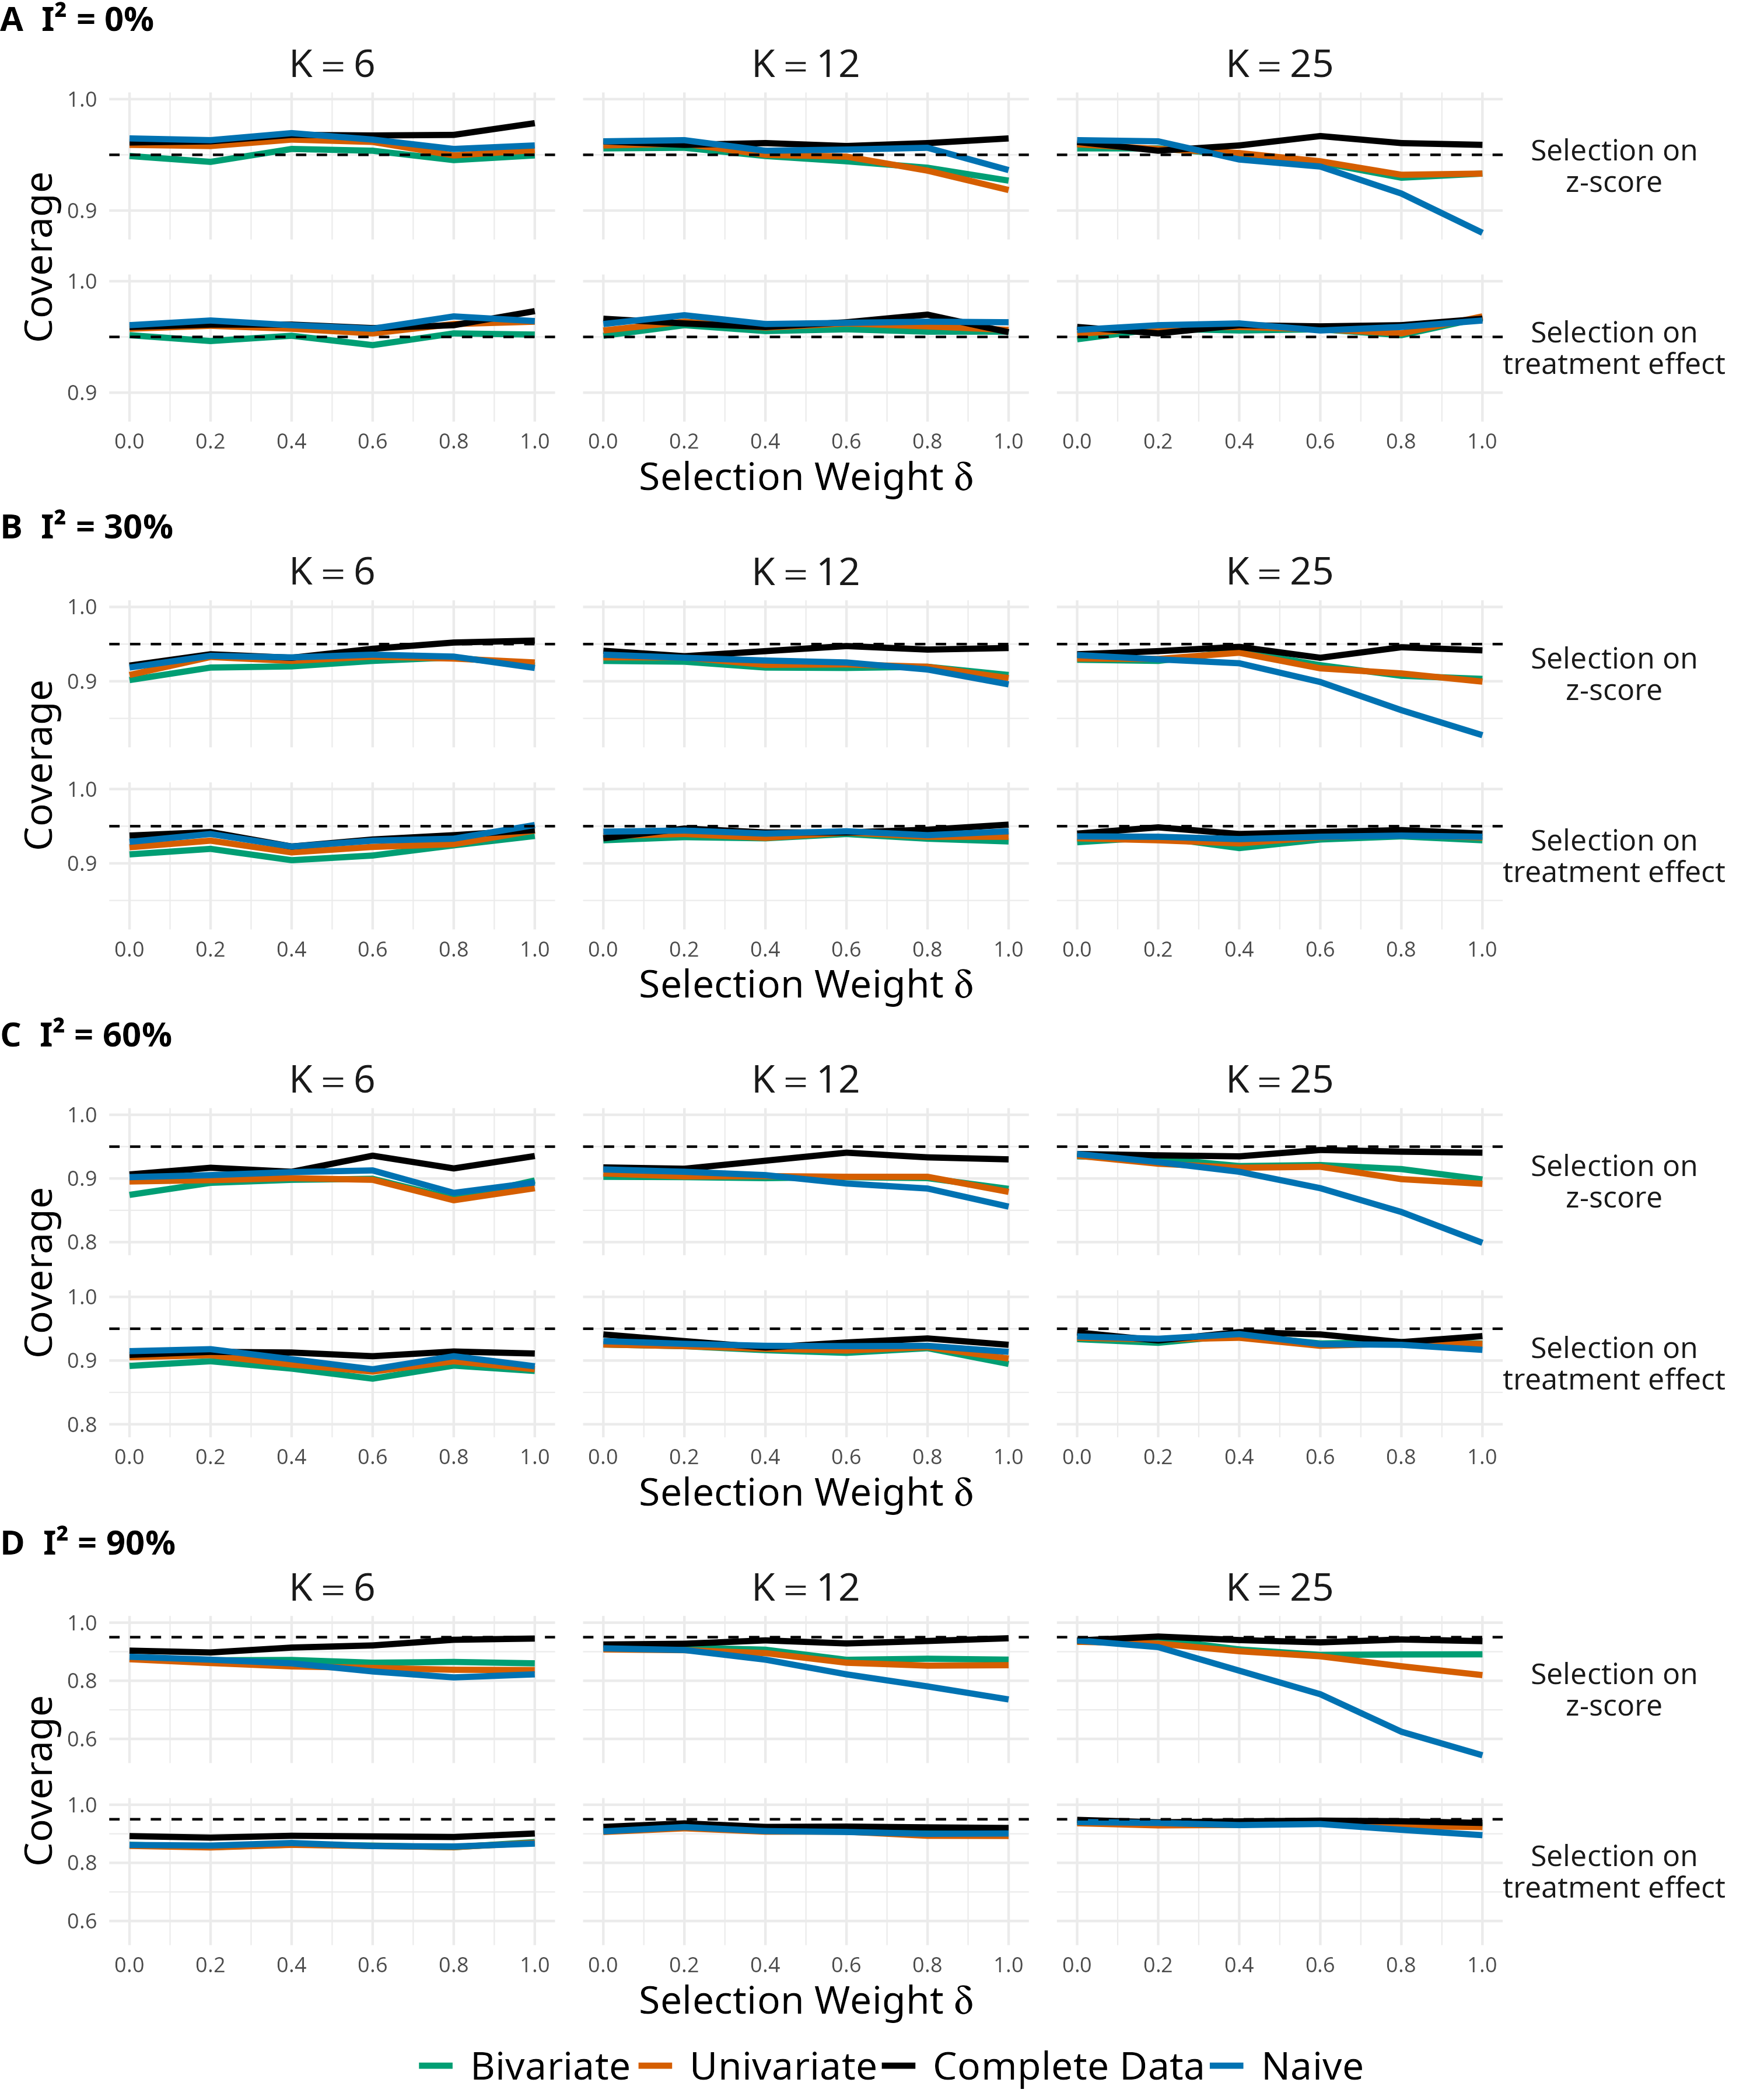
\includegraphics[width = 1\linewidth]{figures/Supp_SimStudy_Coverage_rhoW0.png}
\end{figure}


\clearpage

\subsubsection{\mycolor{Unequal correlation: $\rho_B = 0$, $\rho_W = 0.8$}}
\begin{figure}[!ht]
\centering
\caption{Simulation results for bias of four MA estimates of the treatment effect for outcome 1 under ORB for $\theta_1 = \theta_2 = 0.4$, $\rho_B = 0$, $\rho_W = 0.8$ and $p_1 = 20\%$. Results are shown for varying numbers of studies, heterogeneity levels, selection type, and an increasing selection parameter.}
\label{fig:App_Bias_rhoW08}
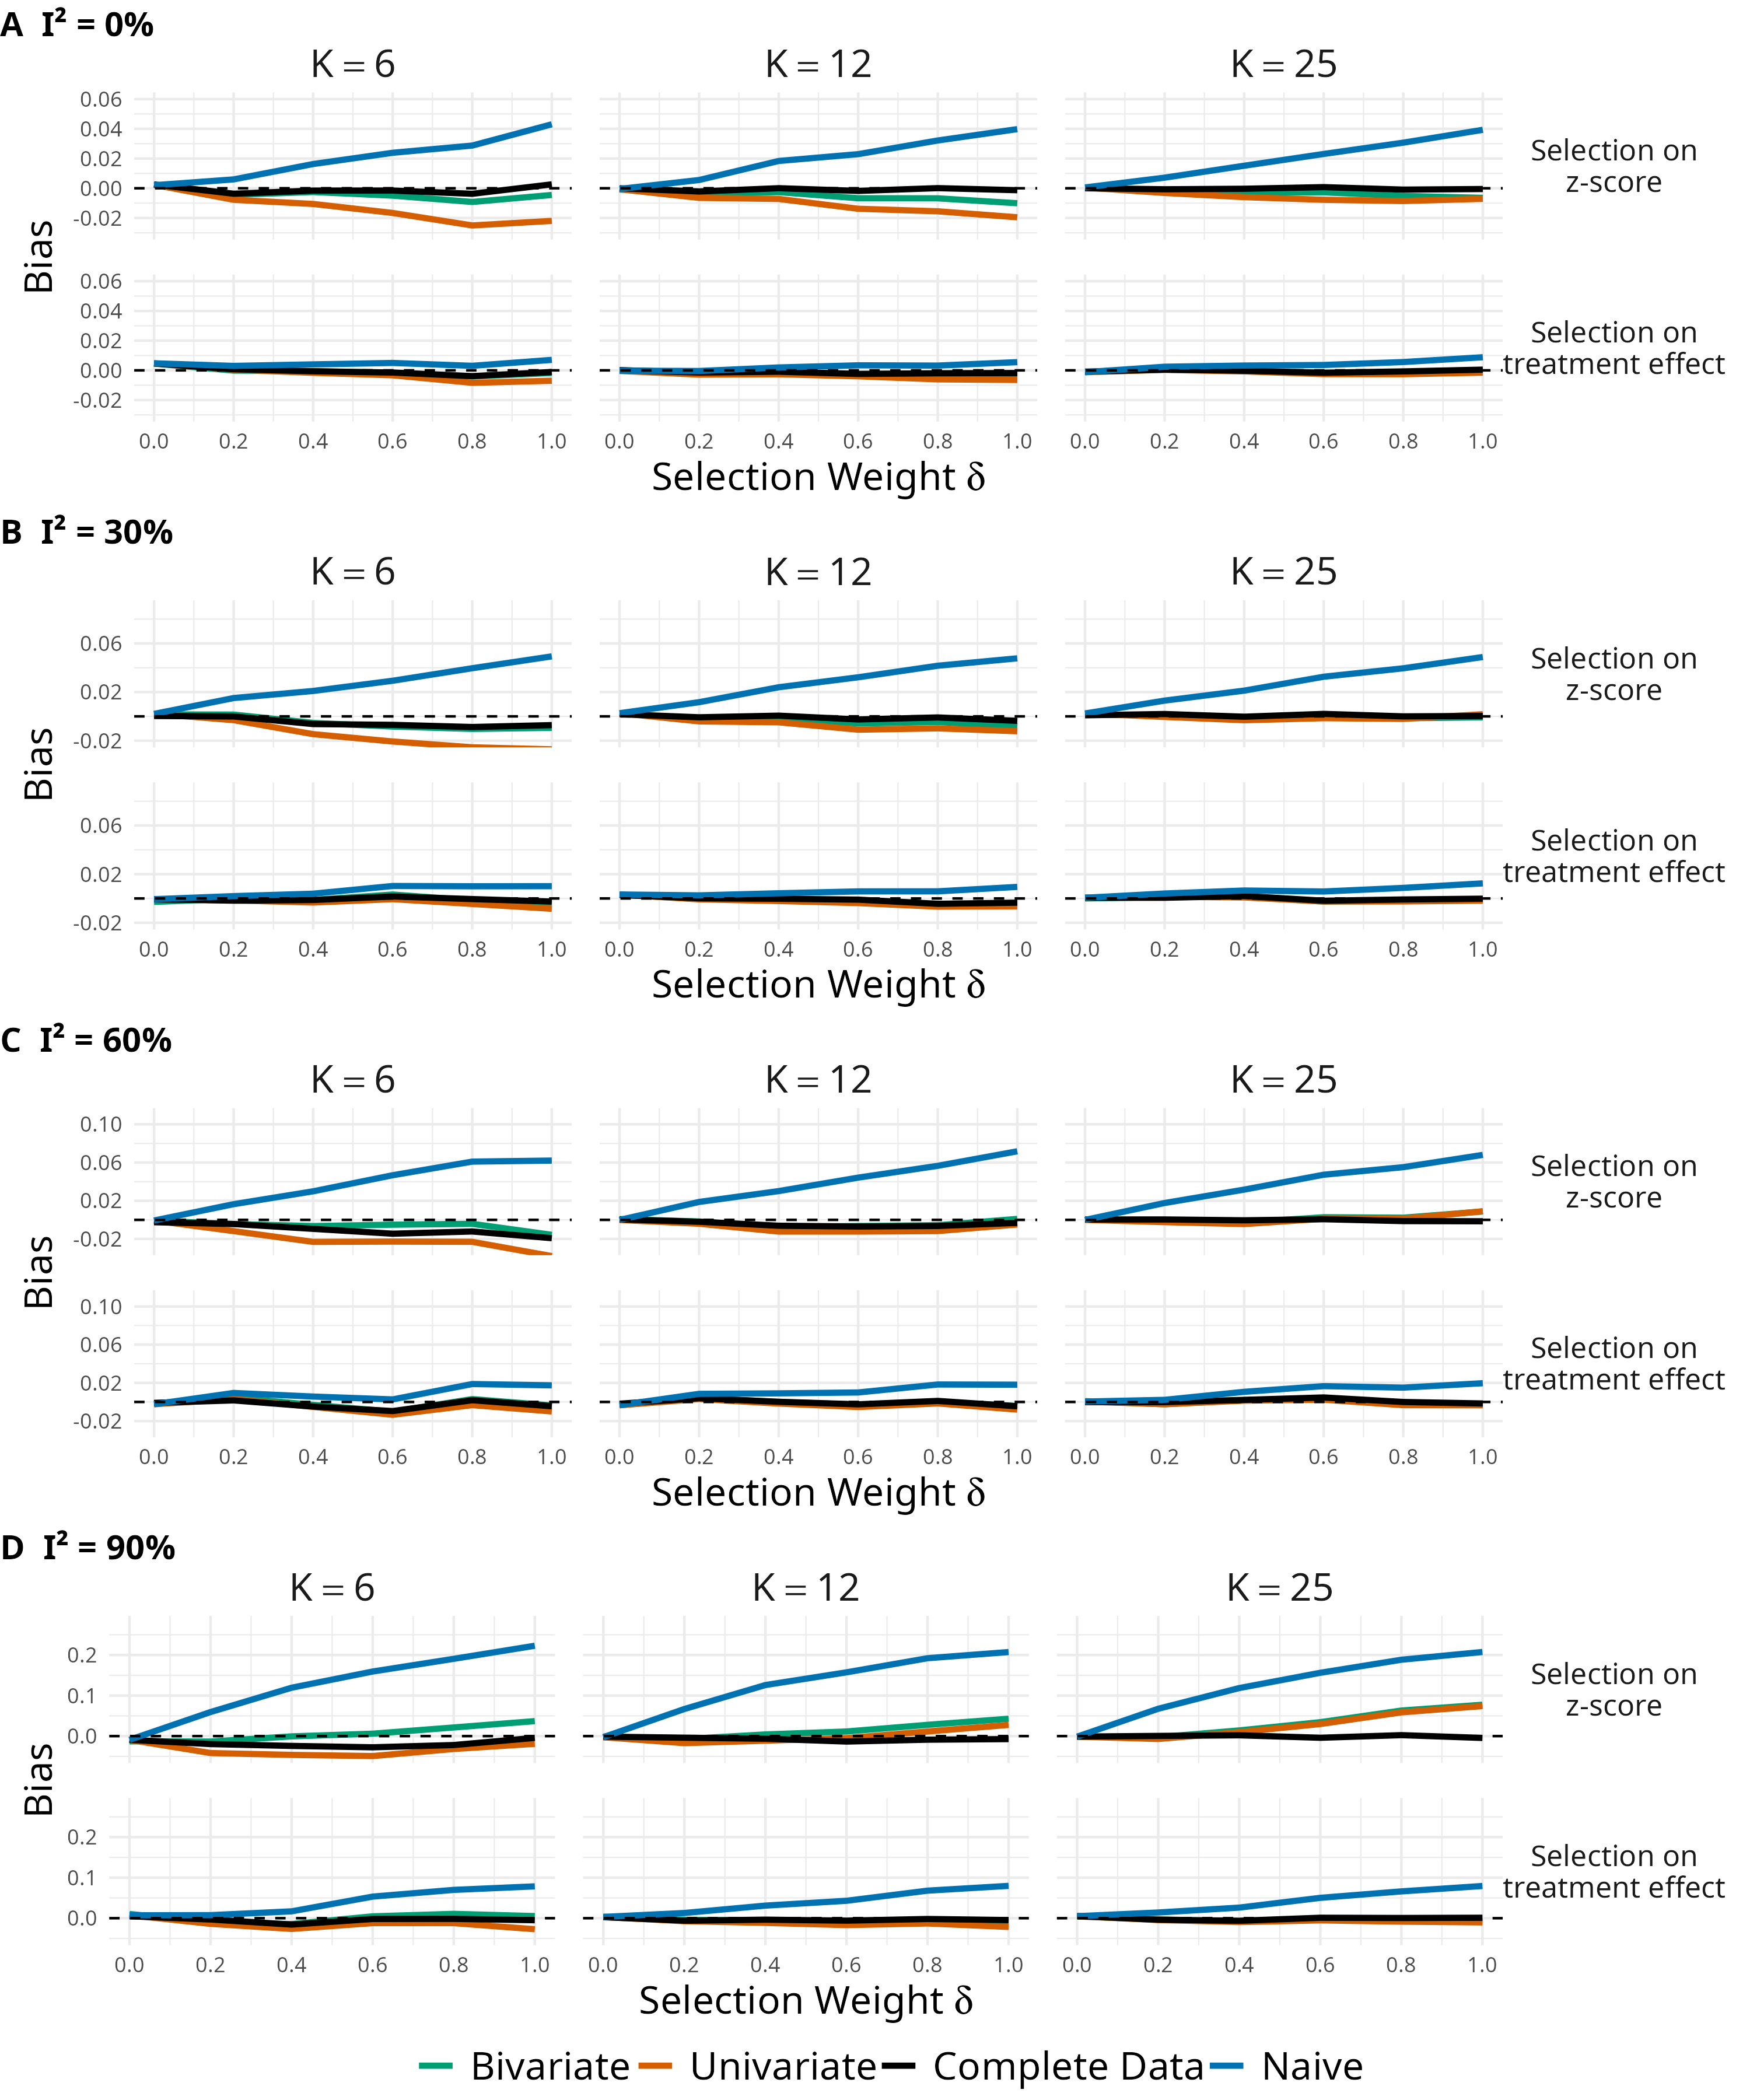
\includegraphics[width = 1\linewidth]{figures/Supp_SimStudy_Bias_rhoW08.png}
\end{figure}

\begin{figure}[!ht]
\centering
\caption{Simulation results for MSE of four MA estimates of the treatment effect for outcome 1 under ORB for $\theta_1 = \theta_2 = 0.4$, $\rho_B = 0$, $\rho_W = 0.8$ and $p_1 = 20\%$. Results are shown for varying numbers of studies, heterogeneity levels, selection type, and an increasing selection parameter.}
\label{fig:App_MSE_rhoW08}
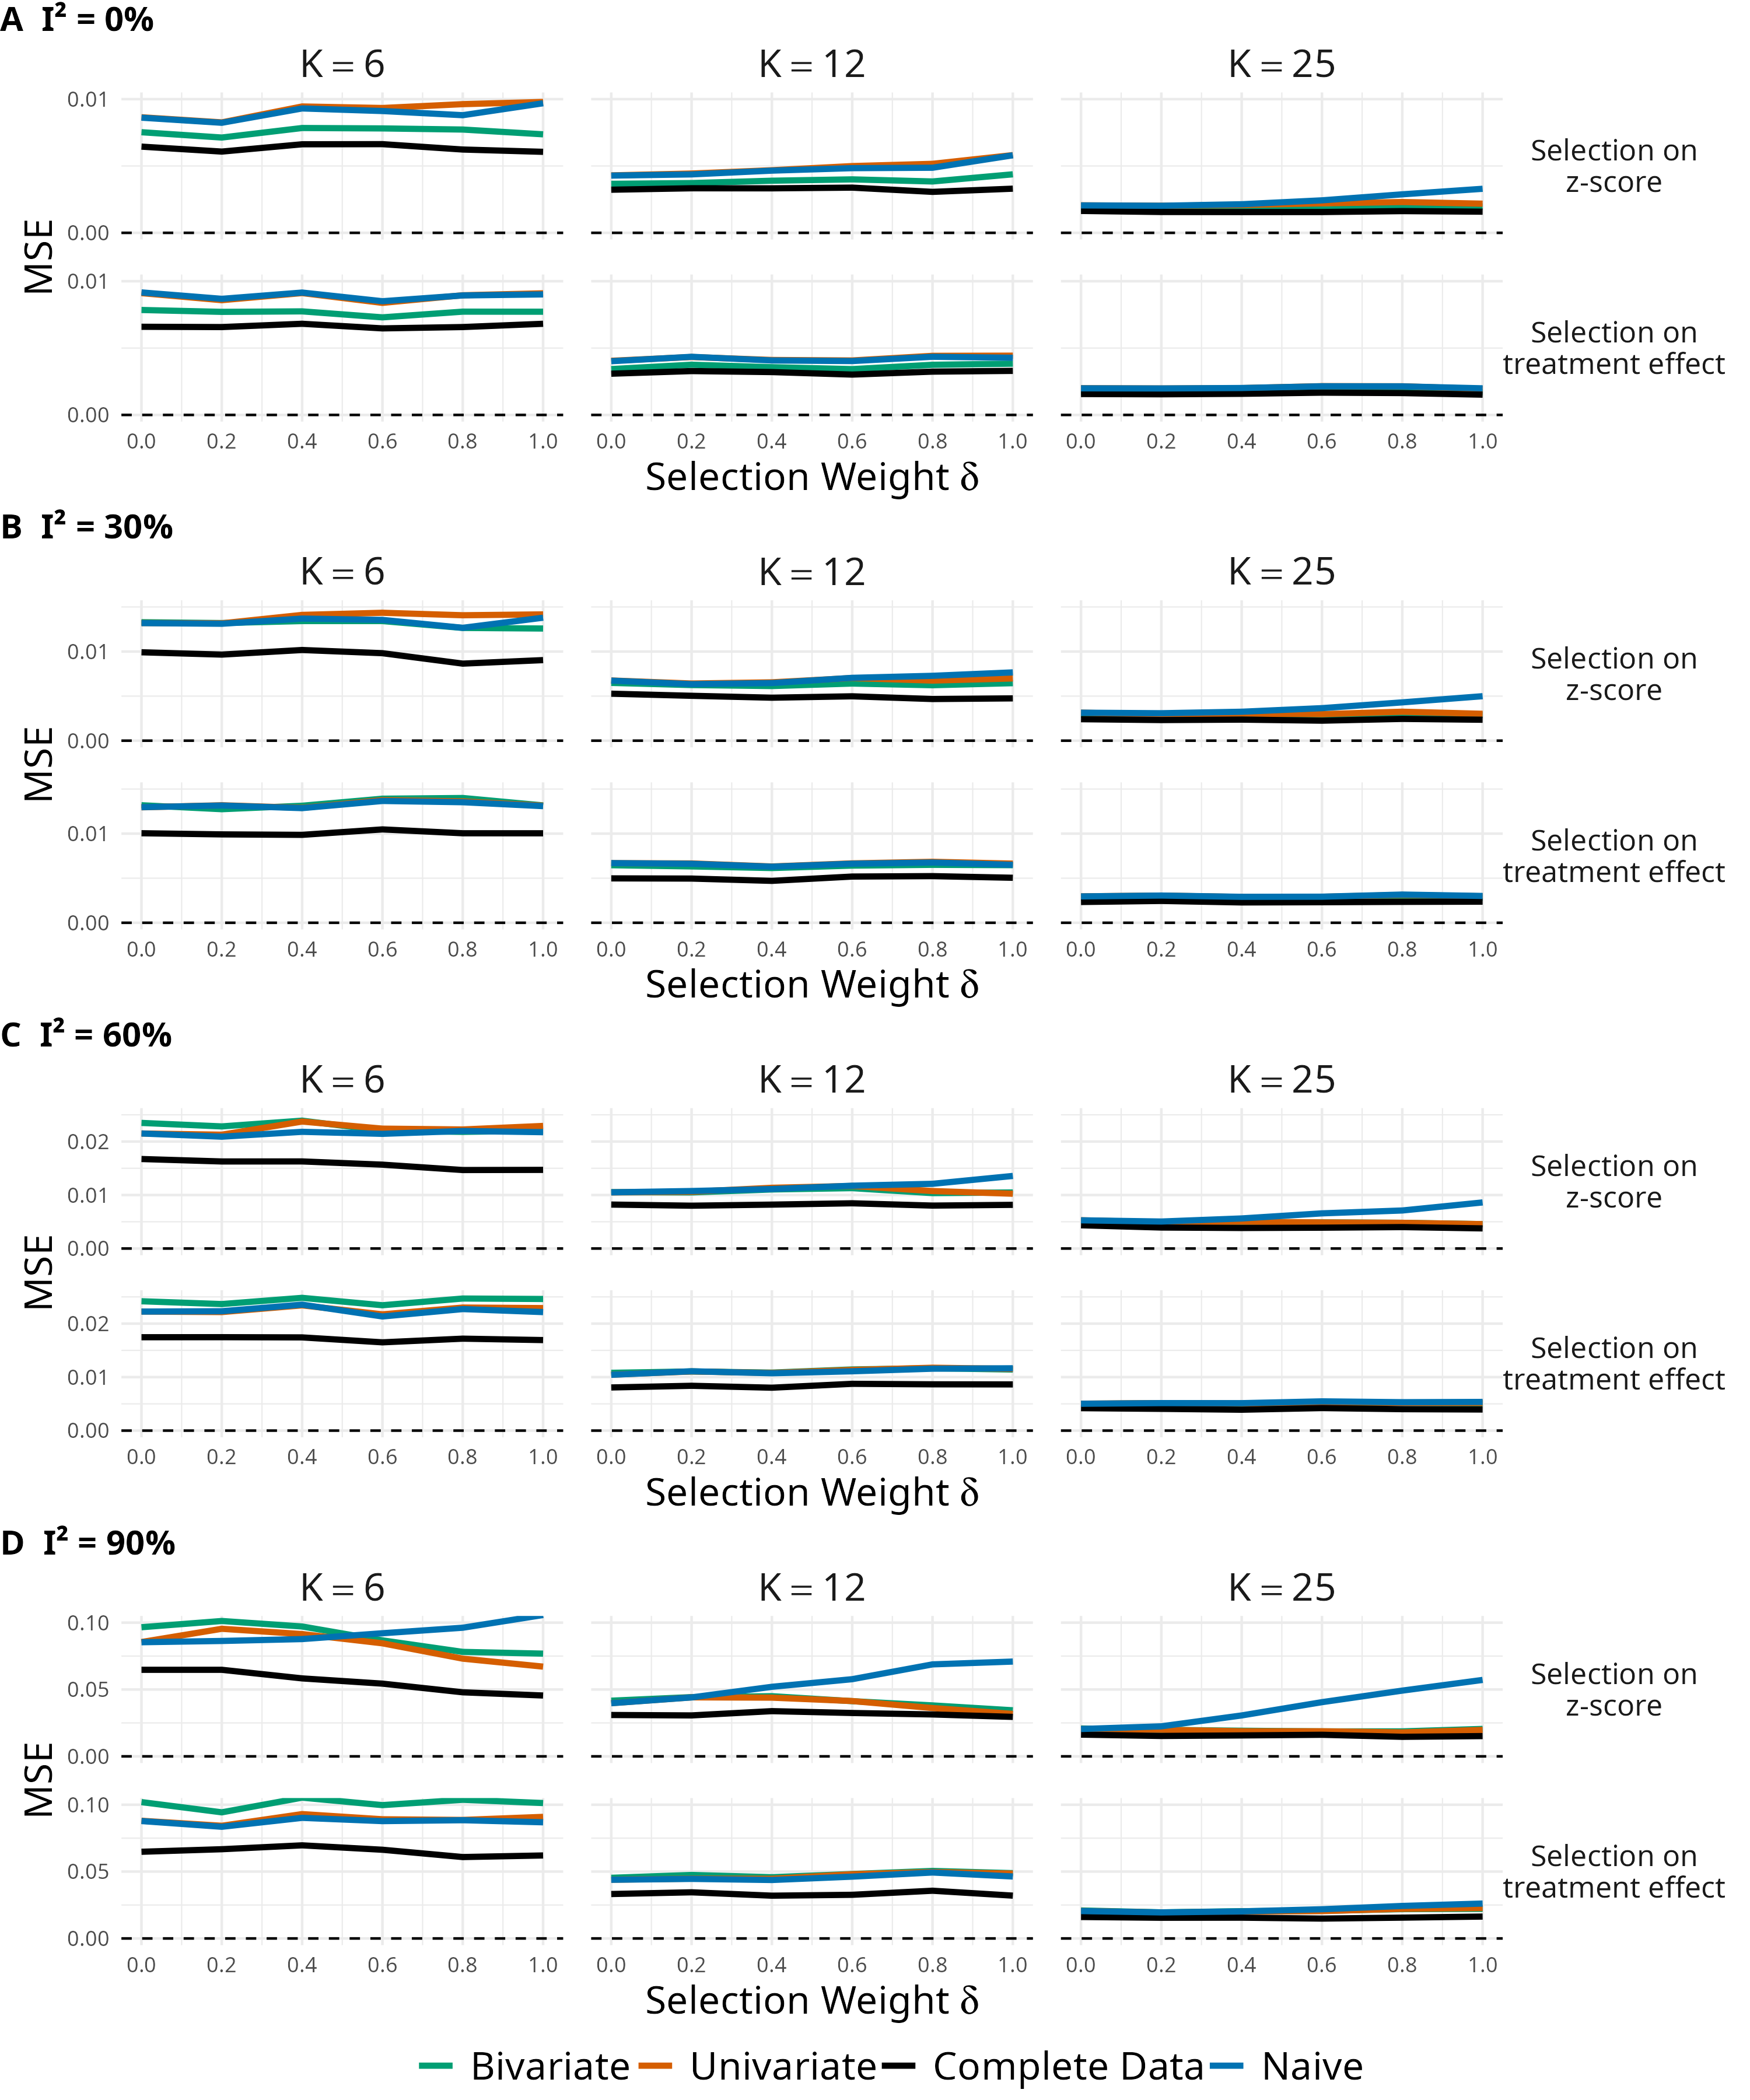
\includegraphics[width = 1\linewidth]{figures/Supp_SimStudy_MSE_rhoW08.png}
\end{figure}

\begin{figure}[!ht]
\centering
\caption{Simulation results for CI width of four MA estimates of the treatment effect for outcome 1 under ORB for $\theta_1 = \theta_2 = 0.4$, $\rho_B = 0$, $\rho_W = 0.8$ and $p_1 = 20\%$. Results are shown for varying numbers of studies, heterogeneity levels, selection type, and an increasing selection parameter.}
\label{fig:App_CIWidth_rhoW08}
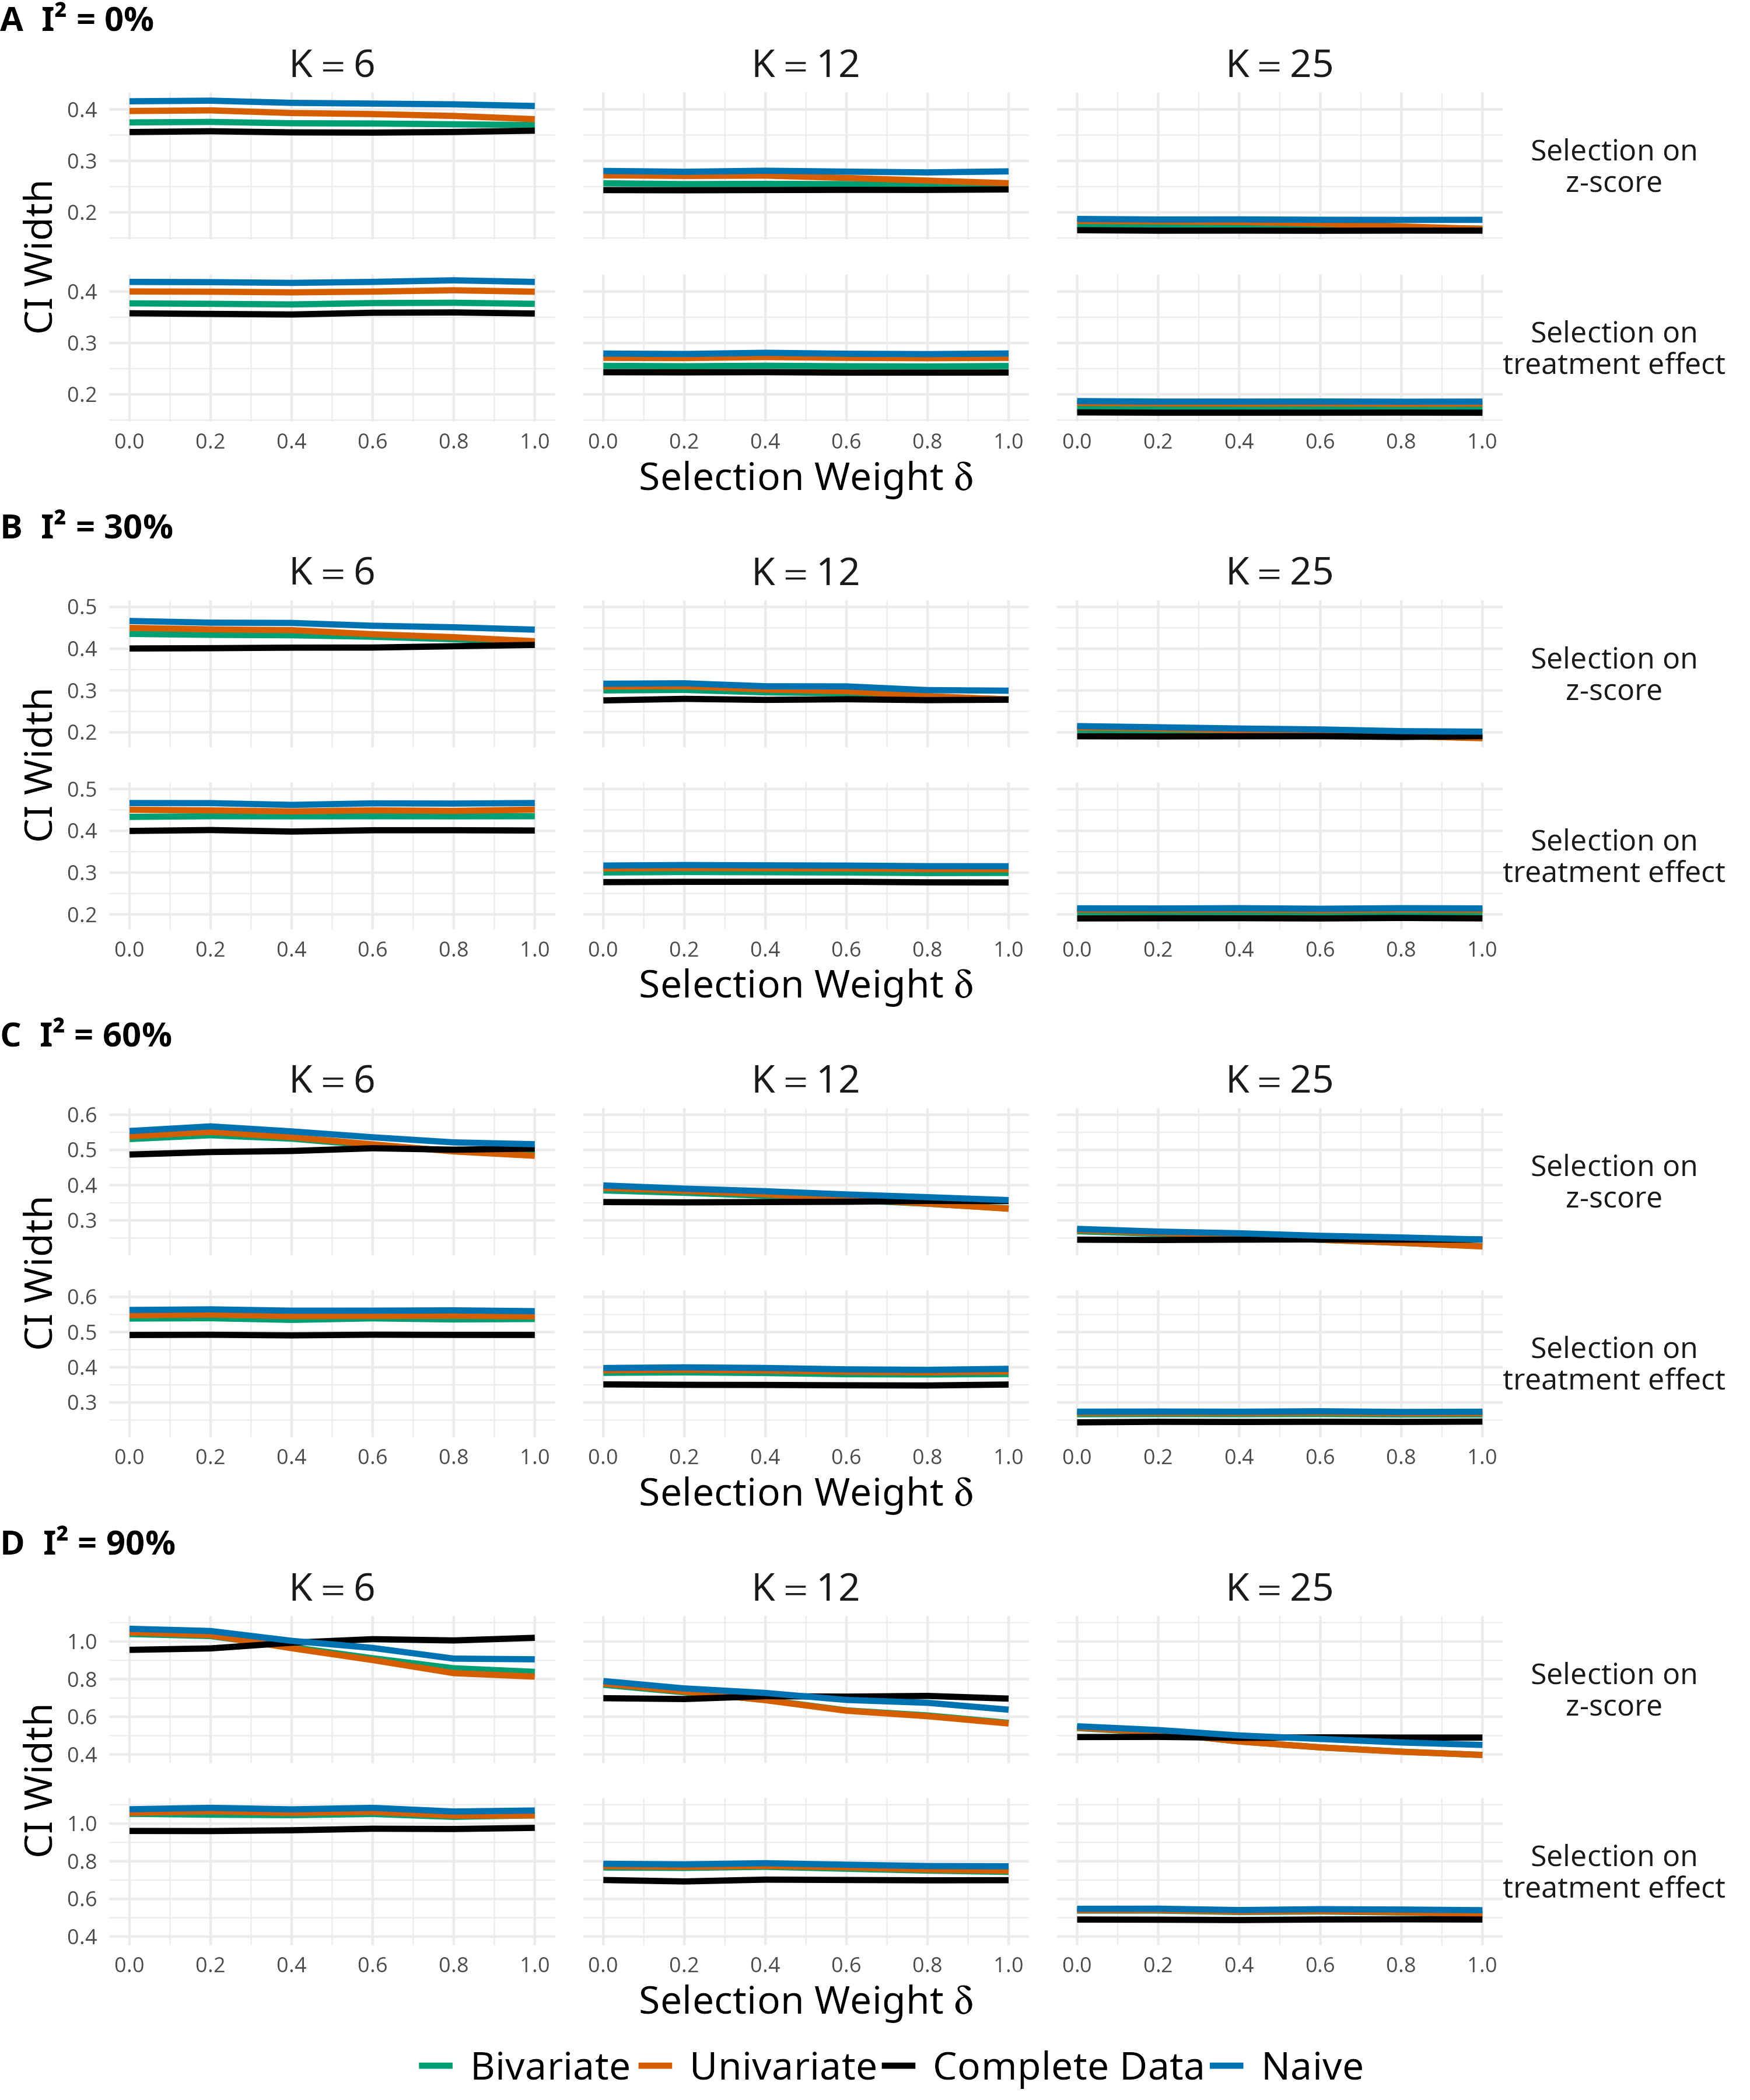
\includegraphics[width = 1\linewidth]{figures/Supp_SimStudy_CIWidth_rhoW08.png}
\end{figure}

\begin{figure}[!ht]
\centering
\caption{Simulation results for coverage of four MA estimates of the treatment effect for outcome 1 under ORB for $\theta_1 = \theta_2 = 0.4$, $\rho_B = 0$, $\rho_W = 0.8$ and $p_1 = 20\%$. Results are shown for varying numbers of studies, heterogeneity levels, selection type, and an increasing selection parameter.}
\label{fig:App_Coverage_rhoW08}
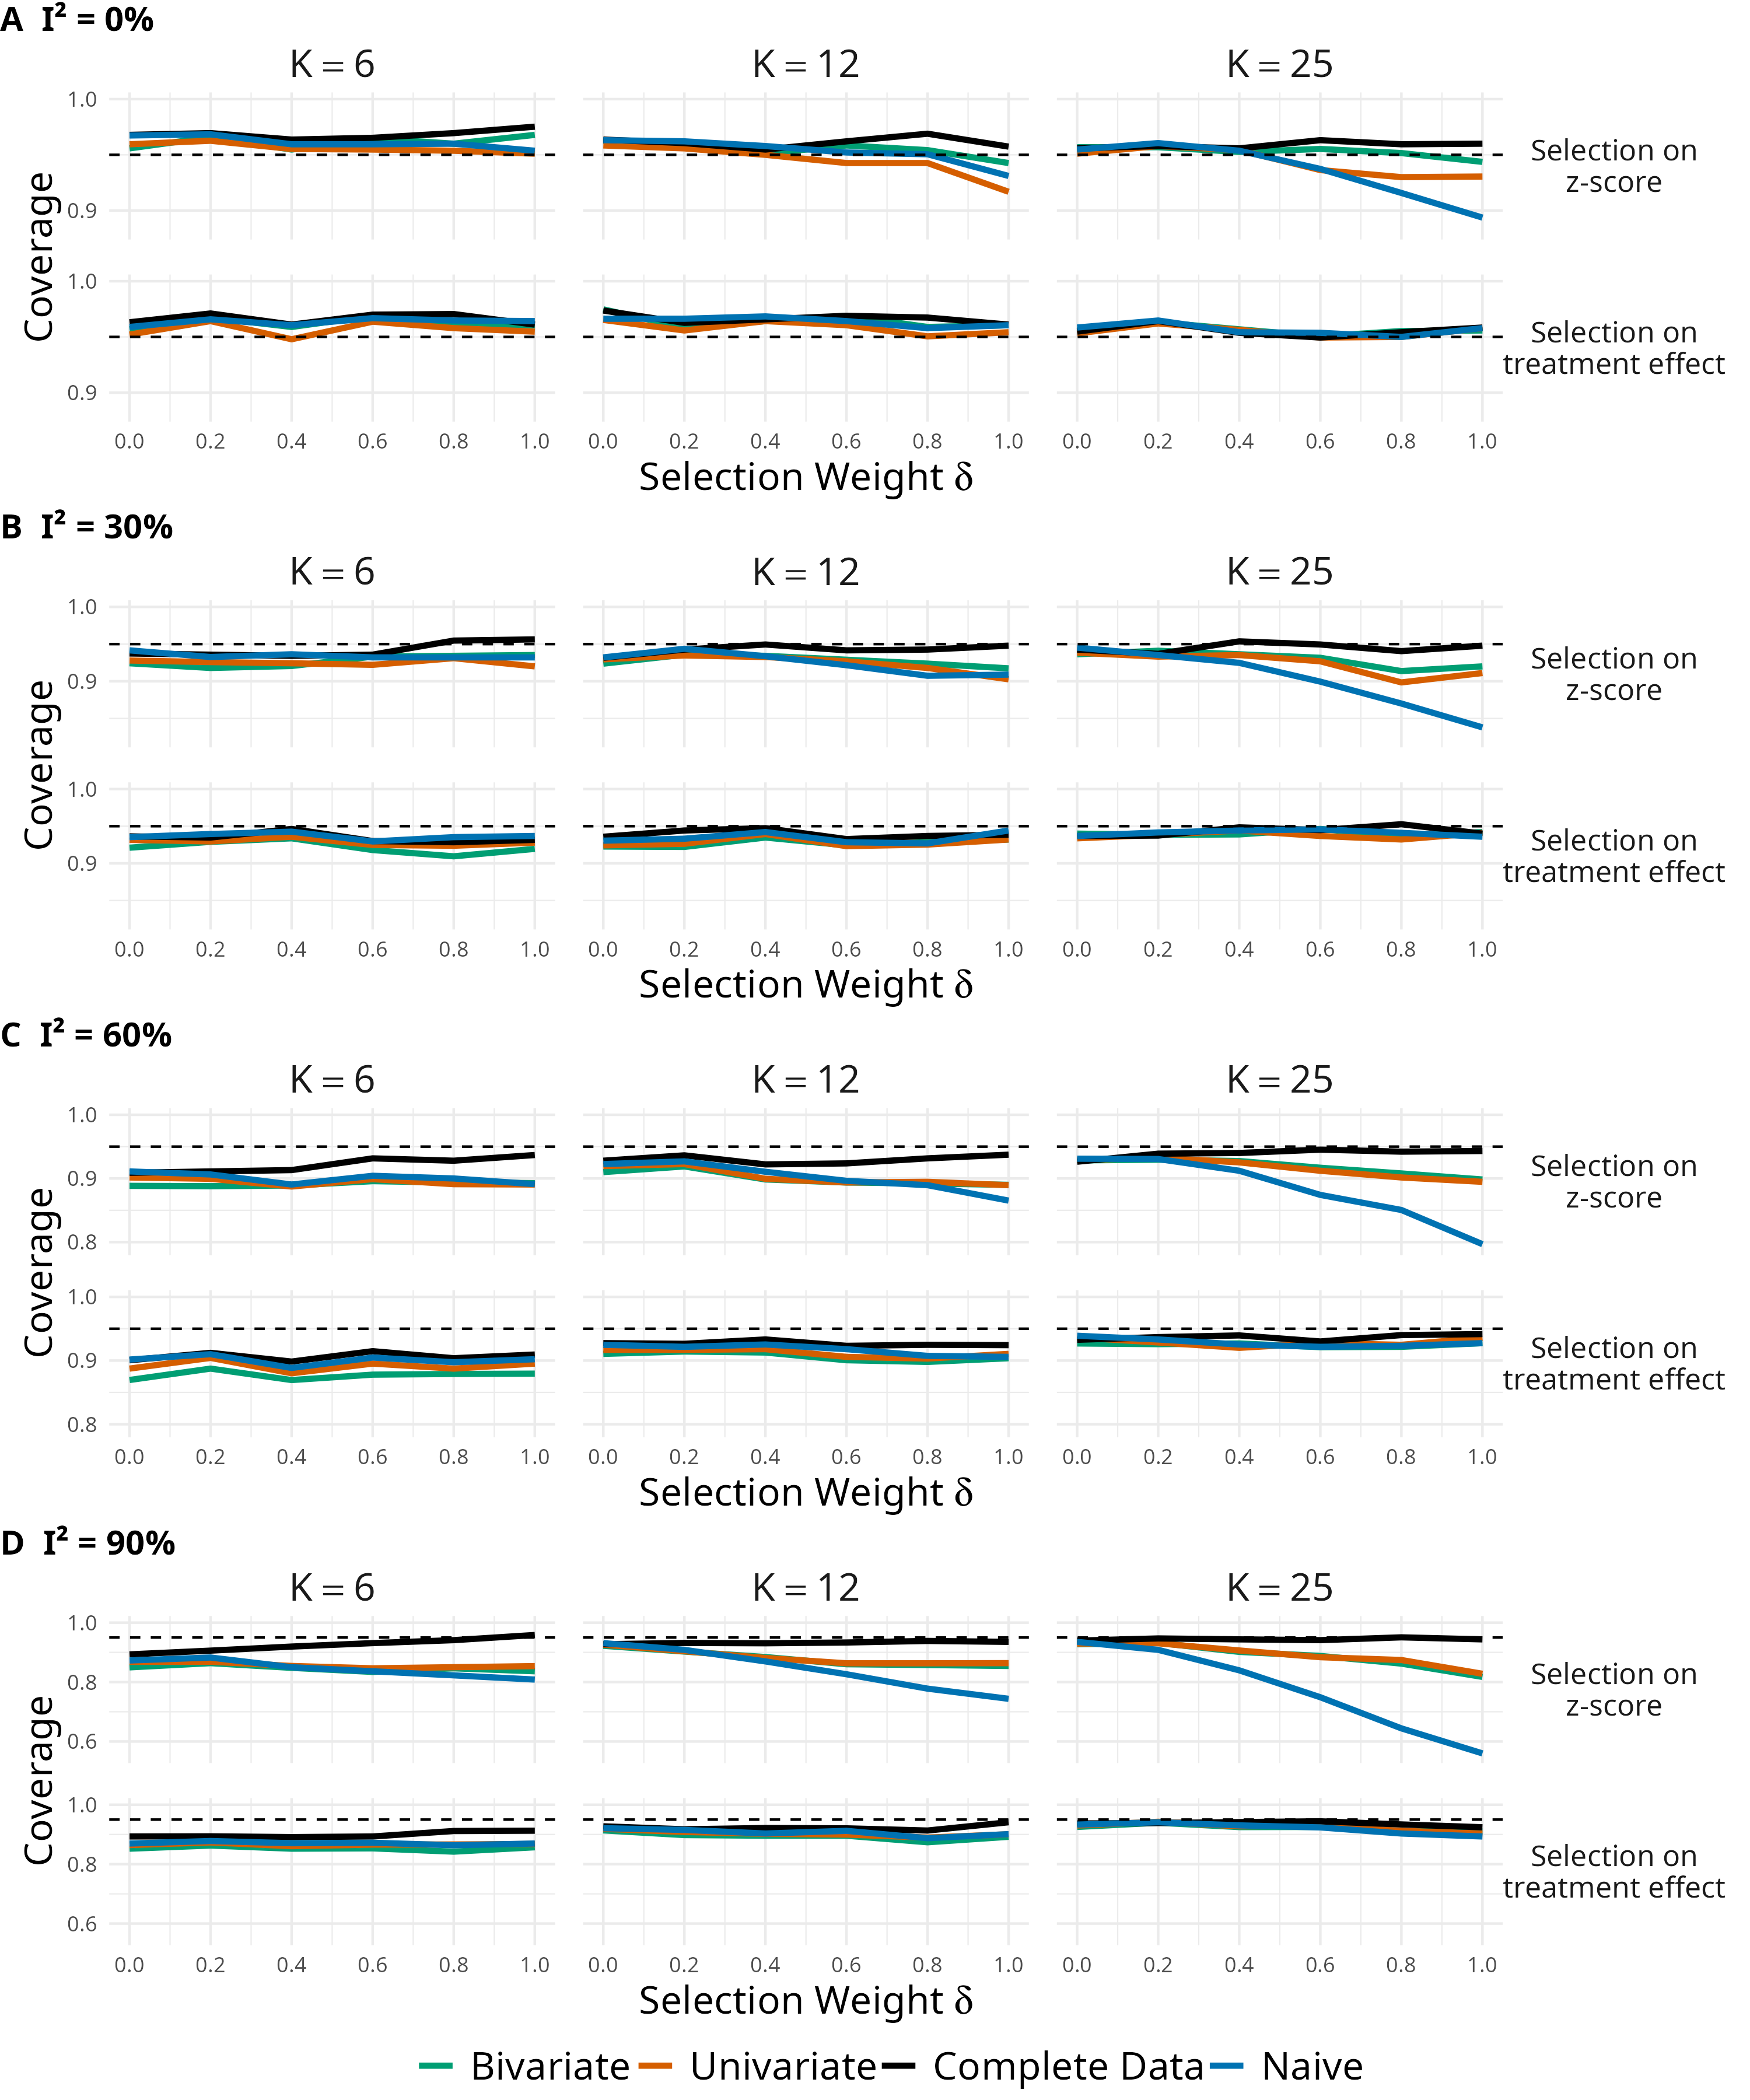
\includegraphics[width = 1\linewidth]{figures/Supp_SimStudy_Coverage_rhoW08.png}
\end{figure}

\clearpage

\subsubsection{\mycolor{Sensitivity analysis over within-study proxy}}
\label{proxy}

\mycolor{In the application, the true within-study correlations were unknown, and we therefore assessed the sensitivity of the results to alternative correlation assumptions. In the simulation study, the true within-study and between-study correlations were specified, allowing us to directly evaluate the accuracy of the Pearson proxy and the consequences of correlation misspecification. We compared the adjustment using (i) the Pearson proxy, (ii) the true $\rho_W$, and (iii) the swapped value, $\rho_B$, as a deliberately misspecified correlation for $\theta_1 = \theta_2 = 0.4$, $K = 25$, $\delta_\text{est} = \delta_\text{sim} \in \{0, 0.5, 1\}$ and $p_1 = 20\%$. The Pearson proxy was close to $\rho_W$ at low heterogeneity and moved towards $\rho_B$ as $I^2$ increased, consistent with it being a variance-weighted combination of both correlations. Figure \ref{fig:App_Bias_proxy} shows that using the Pearson proxy instead of the true within-study correlation does not increase the bias compared to the true $\rho_W$. The swapped value was slightly worse $\rho_W = 0.8$, $\rho_B = 0$ at $I^2 = 0\%$ and $30\%$, and all three coincided at $I^2 = 60\%$ and $90\%$, where within-study covariance contributes little. The coverage shows the same pattern (Figure \ref{fig:App_Coverage_proxy}). The reduction in coverage under selection on the $z$-score at $I^2 = 90\%$ also occurred with the true $\rho_W$ and are therefore not due to the proxy. Also when the proxy is misspecified, coverage is generally similar, with some differences under low heterogeneity. Imposing ORB changed the mean Pearson proxy only slightly (Figure \ref{fig:App_proxy}). These results support the proxy within the scenarios studied, which did not include negative correlations such as the one observed in the application.}

\begin{figure}[!ht]
\centering
\caption{Mean pearson proxy over increasing heterogeneity for complete data and after ORB for $\theta_1 = \theta_2 = 0.4$, $K = 25$, $\delta_\text{est} = \delta_\text{sim} \in \{0, 0.5, 1\} $ and $p_1 = 20\%$.}
\label{fig:App_proxy}
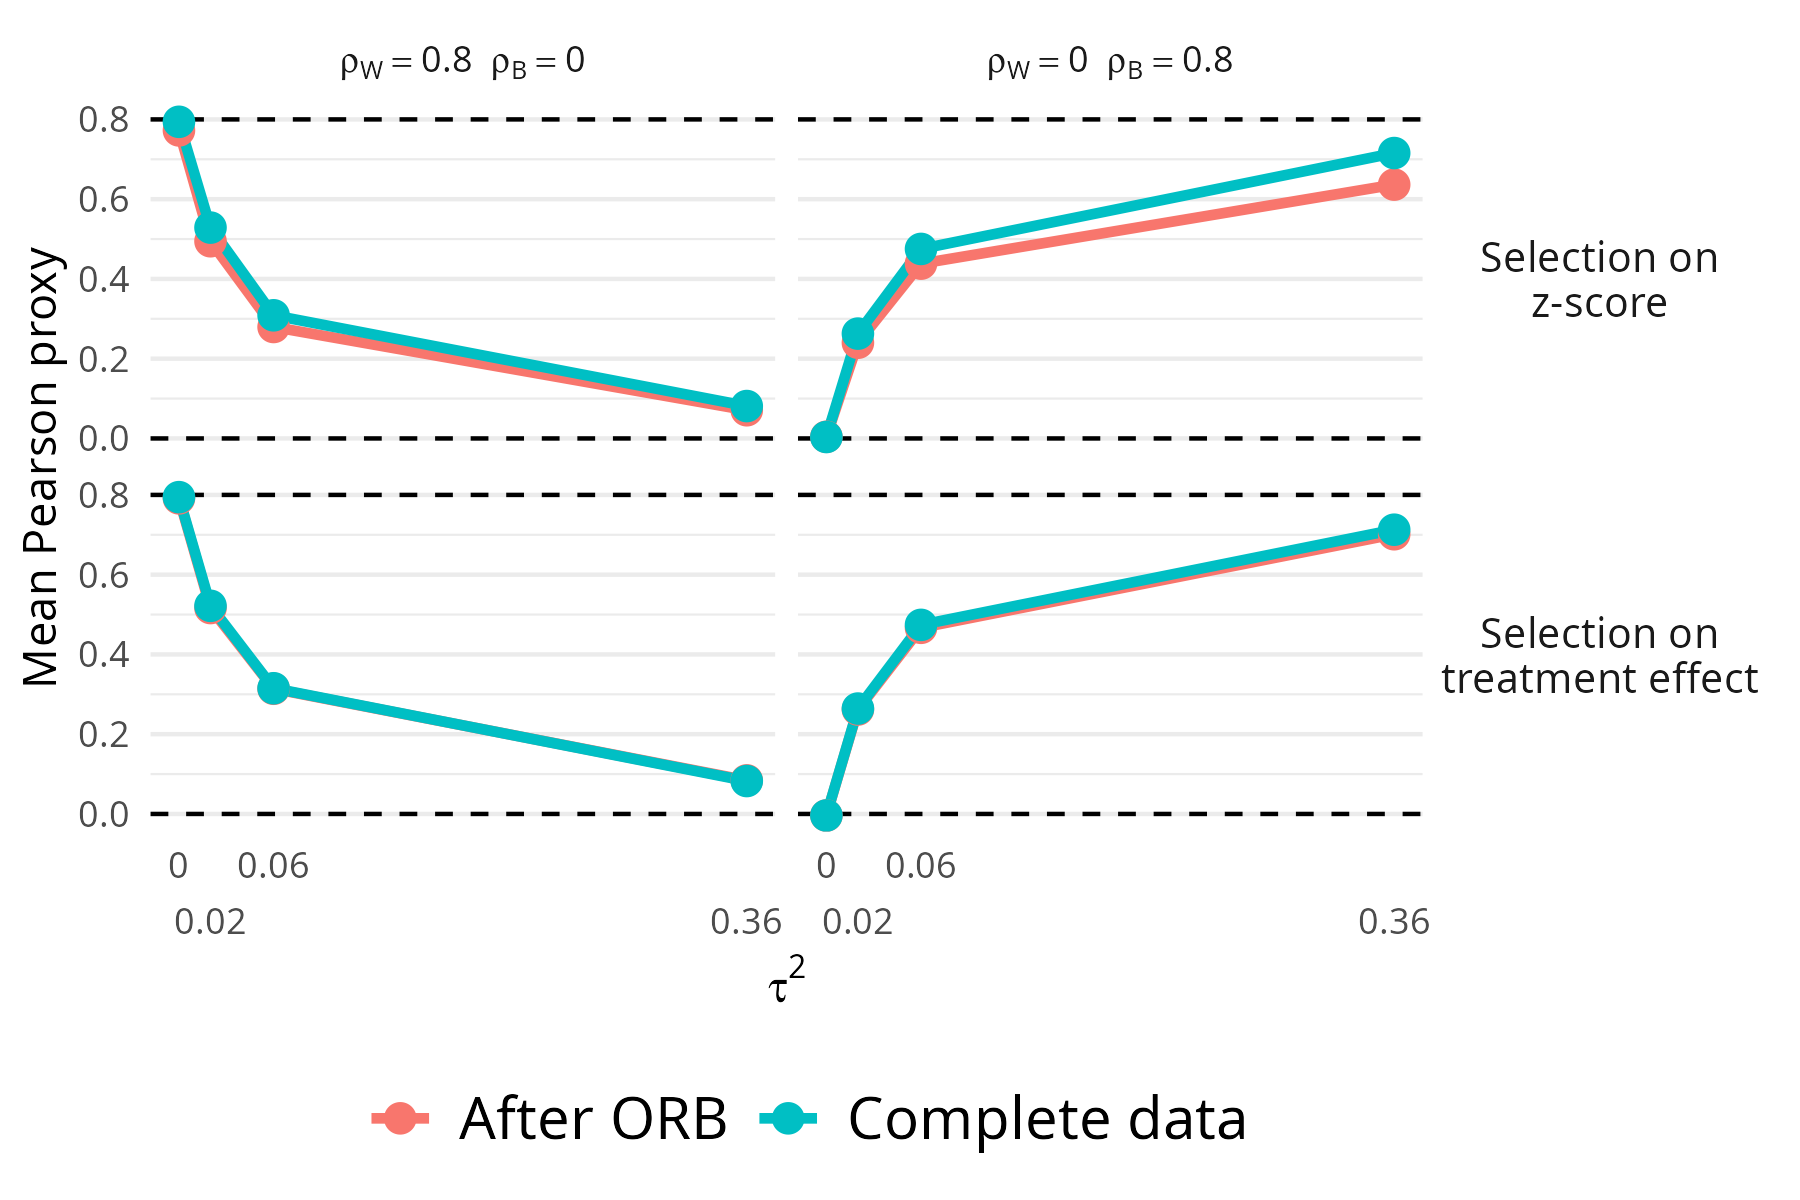
\includegraphics[width = 1\linewidth]{figures/Supp_SimStudy_proxy.png}
\end{figure}

\begin{figure}[!ht]
\centering
\caption{Simulation results for bias of the treatment effect for outcome 1 for bivariate ORB-adjusted estimates under ORB for $\theta_1 = \theta_2 = 0.4$, $K = 25$, $\delta_\text{est} = \delta_\text{sim} \in \{0, 0.5, 1\} $ and $p_1 = 20\%$. Results are shown for varying heterogeneity levels and selection types.}
\label{fig:App_Bias_proxy}
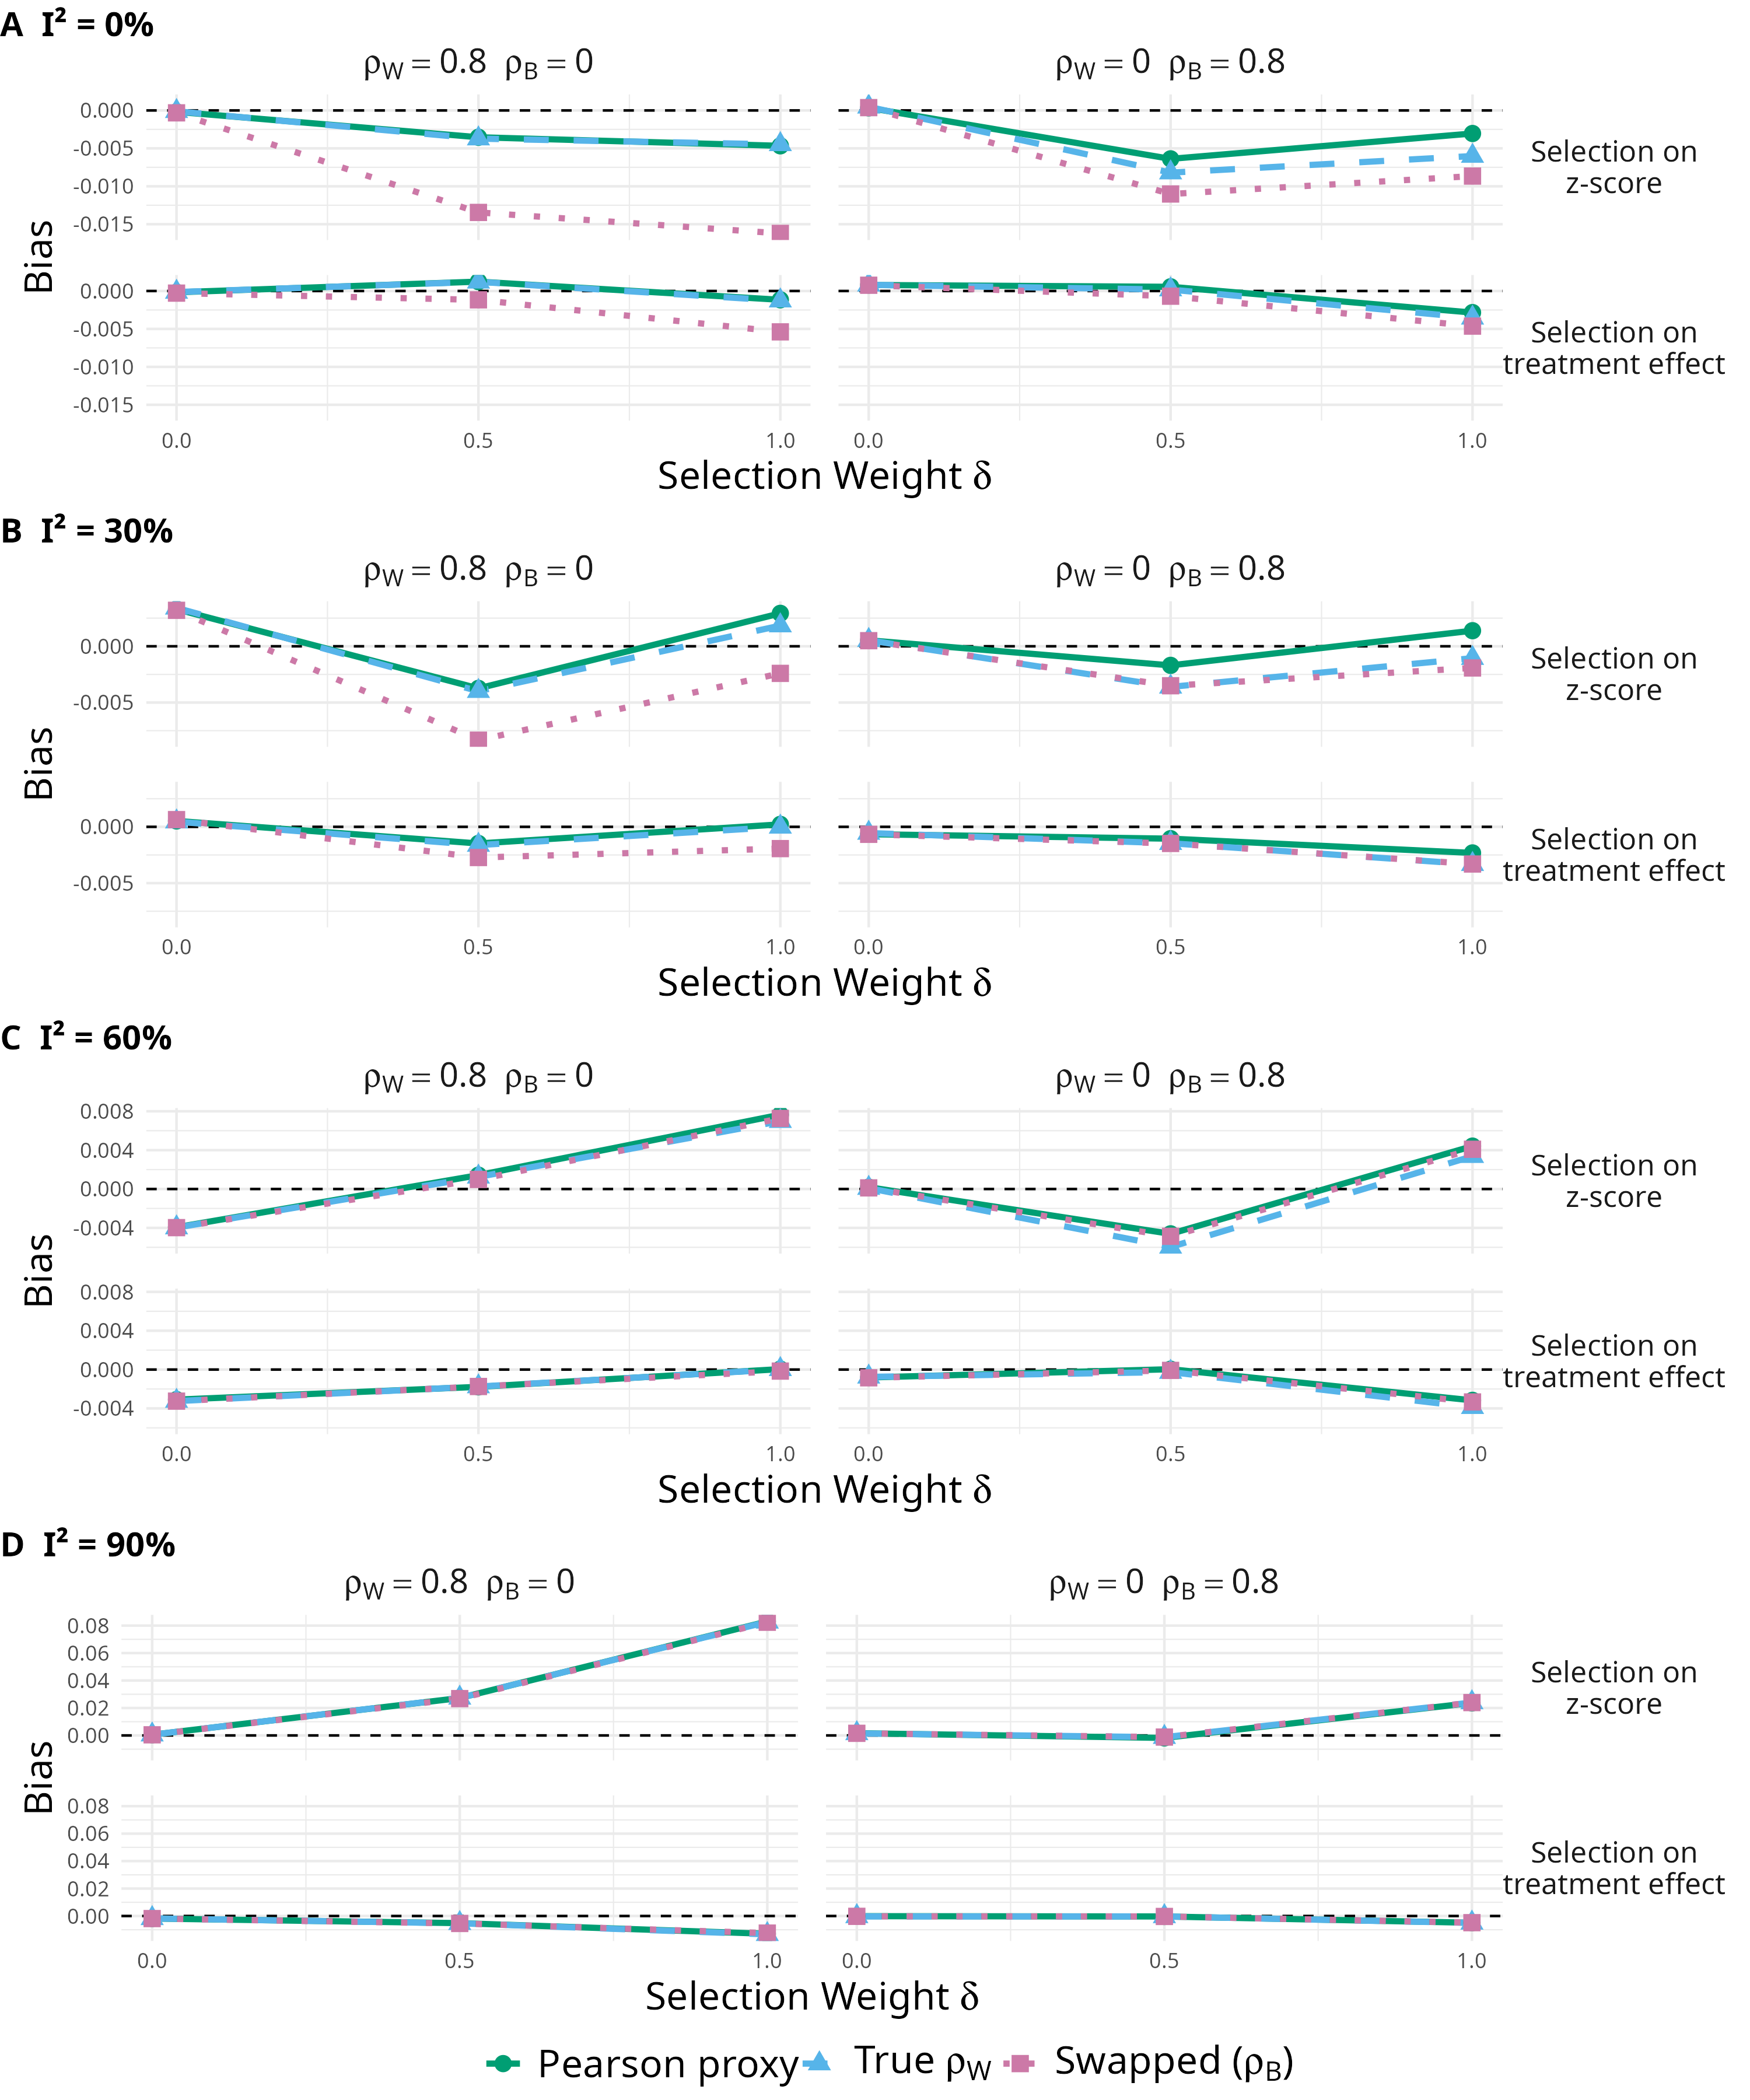
\includegraphics[width = 1\linewidth]{figures/Supp_SimStudy_Bias_proxy.png}
\end{figure}

\begin{figure}[!ht]
\centering
\caption{Simulation results for coverage of the treatment effect for outcome 1 for bivariate ORB-adjusted estimates under ORB for $\theta_1 = \theta_2 = 0.4$, $K = 25$, $\delta_\text{est} = \delta_\text{sim} \in \{0, 0.5, 1\} $ and $p_1 = 20\%$. Results are shown for varying heterogeneity levels and selection types.}
\label{fig:App_Coverage_proxy}
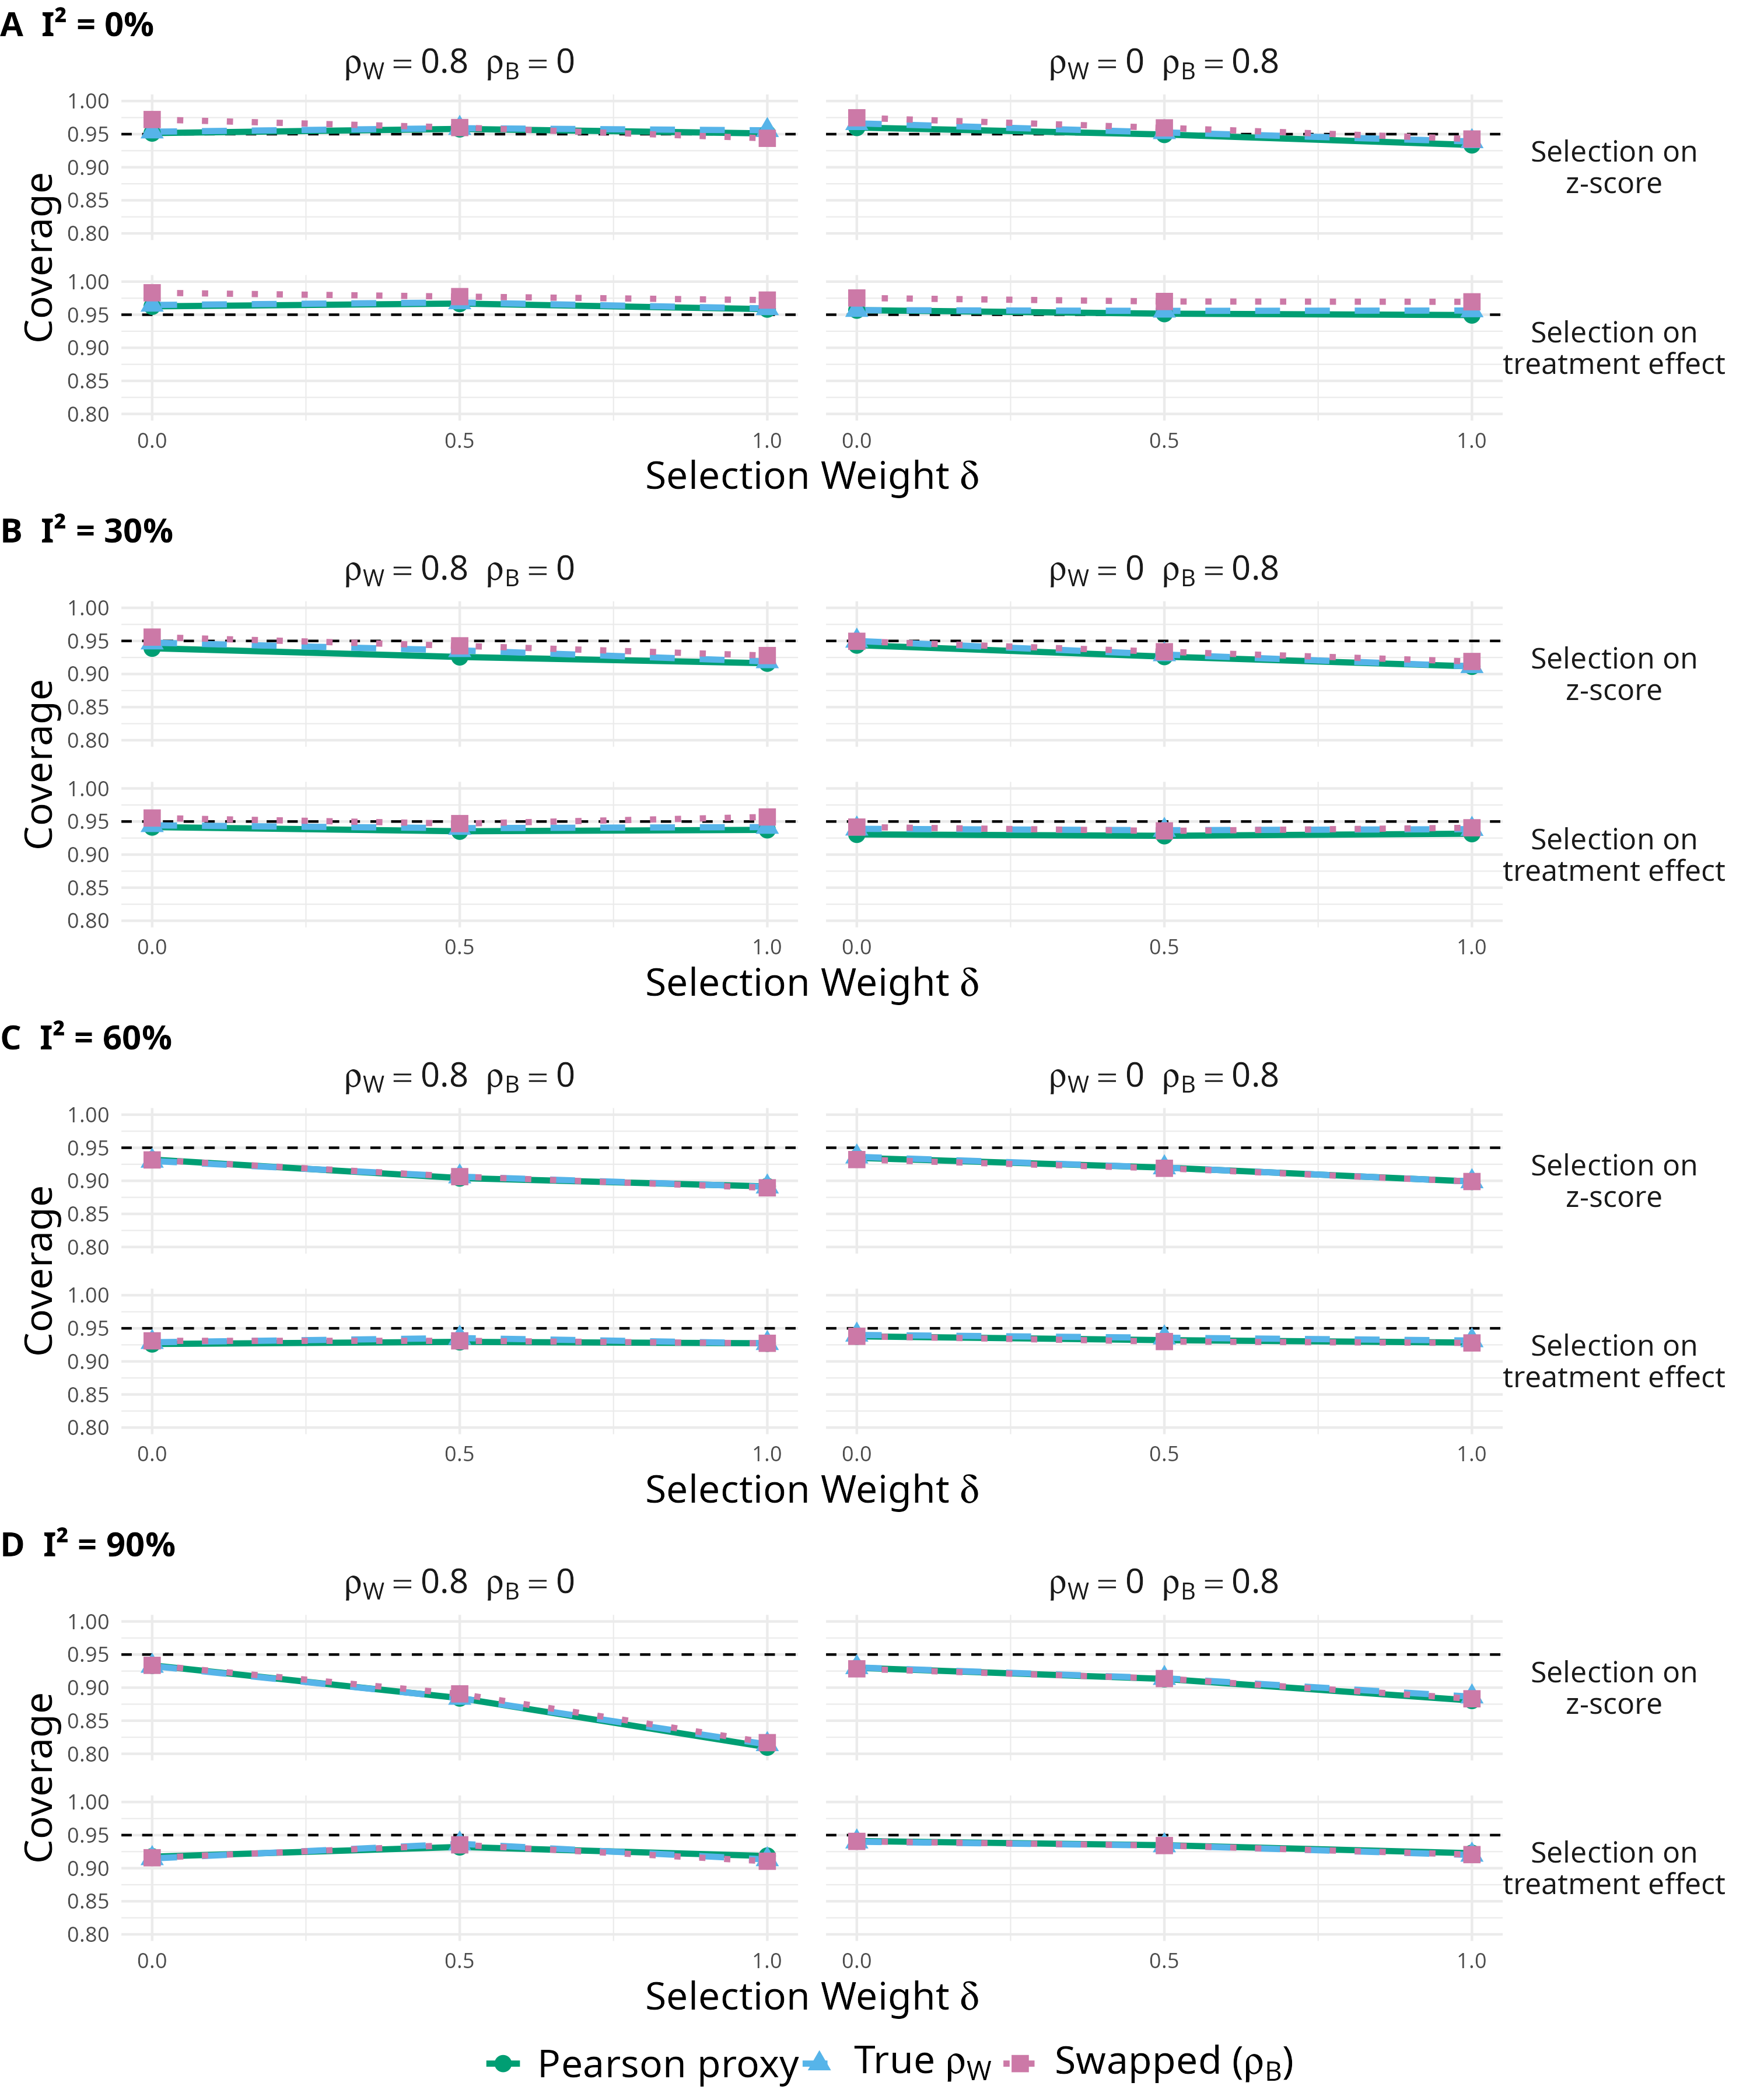
\includegraphics[width = 1\linewidth]{figures/Supp_SimStudy_Coverage_proxy.png}
\end{figure}